%Plantilla basada en "Template for Masters / Doctoral Thesis" (plantilla disponible en writeLaTex) que subió LaTeXTemplates.com

\documentclass[a4paper]{book}
\usepackage[paperwidth=17cm, paperheight=22.5cm, bottom=2.5cm, right=2.5cm]{geometry}
\usepackage{amssymb,amsmath,amsthm} %paquete para símbolo matemáticos
\usepackage[spanish]{babel}
\usepackage[utf8]{inputenc} %Paquete para escribir acentos y otros símbolos directamente
\usepackage{enumerate}
\usepackage{graphicx}
%\usepackage{subfig} %para poner subfiguras
\graphicspath{{Img/}} %En qué carpeta están las imágenes
\usepackage[nottoc]{tocbibind}
\usepackage[pdftex,
            pdfauthor={NOMBRE DEL AUTOR},
            pdftitle={TÍTULO DE LA TESIS},
            pdfsubject={ÁREA DE LA TESIS},
            pdfkeywords={PALABRAS CLAVE},
            pdfproducer={Latex con hyperref},
            pdfcreator={pdflatex}]{hyperref}



\begin{document}

%----------------------------------------------------------------------------------------
%	COMANDOS PERSONALIZADOS
%----------------------------------------------------------------------------------------

%SI TU TESIS TIENE TEOREMAS Y DEMOSTRACIONES, PUEDES DESCOMENTAR Y USAR LOS SIGUIENTES COMANDOS

%\renewcommand{\proofname}{Demostración}
%\providecommand{\norm}[1]{\lVert#1\rVert} %Provee el comando para producir una norma.
%\providecommand{\innp}[1]{\langle#1\rangle} 
%\newcommand{\seno}{\mathrm{sen}}
%\newcommand{\diff}{\mathrm{d}}

%\newtheorem{teo}{Teorema}[section] 
%\newtheorem{cor}[teo]{Corolario}
%\newtheorem{lem}[teo]{Lema}

%\theoremstyle{definition}
%\newtheorem{dfn}[teo]{Definición}

%\theoremstyle{remark}
%\newtheorem{obs}[teo]{Observación}

%\allowdisplaybreaks



%----------------------------------------------------------------------------------------
%	PORTADA
%----------------------------------------------------------------------------------------

\title{TesisMaxi} %Con este nombre se guardará el proyecto en writeLaTex

\begin{titlepage}
\begin{center}

\textsc{\Large Facultad de Inveniería \- Universidad Nacional de Mar del Plata}\\[4em]

\vspace{4em}

\textsc{\huge \textbf{Sistemas Complejos, Ruidos Discretos y su implementación en FPGA}}\\[4em]

\textsc{\large Tesis}\\[1em]

\textsc{para obtener el título de}\\[1em]

\textsc{Doctor en Ingeniería con Orientación en Electrónica}\\[1em]

%\textsc{presenta}\\[1em]

\textsc{\Large Maximiliano Antonelli}\\[1em]

%\textsc{\large Asesor: NOMBRE}

\end{center}

\vspace*{\fill}
\textsc{Mar del Plata, Argentina \hspace*{\fill} 2016}

\end{titlepage}

%----------------------------------------------------------------------------------------
%	DEDICATORIA
%----------------------------------------------------------------------------------------

\pagestyle{empty}
\frontmatter

\chapter*{}
\begin{flushright}
\textit{A Sonia y Eduardo, que hicieron la mejor versión de mí que pudieron.\\
A Lorena, que sigue intentándolo.\\
A Giuliana y Luca, que les sale sin querer.}
\end{flushright}

%----------------------------------------------------------------------------------------
%	AGRADECIMIENTOS
%----------------------------------------------------------------------------------------

\chapter*{Agradecimientos}
%\markboth{AGRADECIMIENTOS23}{AGRADECIMIENTOS} % encabezado 

¡Muchas gracias a todos!

\tableofcontents


%----------------------------------------------------------------------------------------
%	TESIS
%----------------------------------------------------------------------------------------
\mainmatter %empieza la numeración de las páginas
\pagestyle{headings}

%  Incluye los capítulos en el folder de capítulos

Los sistemas dinámicos son sistemas que evolucionan en el tiempo.
En la práctica, sólo es posible medir alguna funcional del sistema bajo estudio, generalmente una serie de tiempo escalar $X(t)$ la cual puede ser función de las variables $V=\{ v_1, v_2,\cdots, v_k\}$ que describe la dinámica subyacente (por ejemplo $dV/dt=f(V)$).
Tratamos de inferir propiedades de un sistema no conocido a partir del análisis de los datos guardados de variables observacionales.
¿Cuánta información revelan estos datos sobre la dinámica del sistema o procesos subyacentes?

El contenido de información de un sistema se evalúa típicamente mediante una función de distribución de probabilidades (PDF) $P$ que describe la distribución de alguna cantidad mensurable u observable, generalmente una serie temporal $X(t)$.
Podemos definir los cuantificadores de la Teoría de la Información como medidas capaces de caracterizar las propiedades relevantes de las PDFs asociadas a estas series temporales, y de esta manera debemos extraer juiciosamente información sobre el sistema dinámico en estudio.
Estos cuantificadores representan métricas en el espacio de PDFs para conjuntos de datos, permitiendo comparar diferentes conjuntos y clasificarlos de acuerdo a sus propiedades de procesos subyacentes, de manera amplia, estocástica vs. determinística.

En nuestro caso, nos interesa la dinámica caótica.
Por lo tanto, nos centramos en las métricas que toman en cuenta el orden temporal de las observaciones de forma explícita; es decir, el enfoque es fundamentalmente de naturaleza \textit{causal} y \textit{estadística}.
En un enfoque puramente estadístico, las correlaciones entre los valores sucesivos de las series temporales se ignoran o simplemente se destruyen a través de la construcción de la PDF; mientras que un enfoque causal se centra en las PDFs de secuencias de datos.
Además, los exponentes de Lyapunov permiten analizar los datos de un punto de vista topológico y brindan una valiosa información acerca de la caoticidad del sistema.

En este Capítulo se presenta al Máximo Exponente de Lyapunov (MLE) como un detector de caos en la Sección \ref{secMLE}, para luego presentar un caso de aplicación de un algoritmo de búsqueda de caos.
Este algoritmo fue presentado en \cite{CASE2013} y muestra la factibilidad de la búsqueda automática de caos con algoritmos eurísticos basados en el  MLE.
Otras publicaciones en este campo son dos implementaciones en FPGA de distintos algoritmos.
En \cite{DeMicco2013} se presenta una implementación en hardware de un estimador del MLE.
Esta técnica precisa tener acceso a las entradas y salidas del sistema analizado, es decir, introducir las CIs del sistema.
Además, forma parte del sistema presentado en \cite{CASE2013}.
En \cite{LASCAS2017} se presentó otro algoritmo que estima el MLE a partir de una serie de datos, es decir que no precisa acceso al sistema.
Esta última aproximación es más realista, ya que generalmente uno sólo tiene acceso a una serie temporal observable del sistema.

En la segunda Sección de este Capítulo se presentan una serie cuantificadores de aleatoriedad provenientes de la Teoría de la Información.
Estos cuantificadores se utilizan luego a través del resto de esta tesis como una herramienta de análisis, con ellos se evalúa la calidad de los generadores de números aleatorios.
Luego se muestran los resultados presentados en \cite{Antonelli2016}, en donde se implementaron estas herramientas en FPGA.
La implementación de estos cuantificadores surge como una solución práctica, así es posible medir la calidad de los generadores en la misma plataforma, sin la necesidad de extraer los datos y medirlos en una computadora.
Aprovechando la disponibilidad de entradas analógicas en el kit de desarrollo, al diseño se le agregó la posibilidad de medir señales analógicas externas.
Cuando se midieron señales de prueba bien conocidas, los resultados mostraron ciertos corrimientos de los valores esperados debido a la contaminación con ruido aditivo (AWGN) y a la limitación en la banda de paso inherentes a todo sistema analógico.
Esto abre la inquietud de caracterizar el comportamiento de los cuantificadores frente a estos dos factores, por lo que se presentó un trabajo al respecto en \cite{TREFEMAC2016}.
Los resultados de este estudio se muestran en la Sección \ref{ssec:TDdS}.
\thispagestyle{empty}

\chapter{Generadores de Números Aleatorios}

%%%%%%%%%%%%%%%%%%%%%%%%%%%%%%%%%%%%%%%%%%%%%%%%%%%%%%%%%%%%%%%%%%%%%%%%%%%%%
\section{Cripto-Codificación caótica Variante en el tiempo}

\subsection{Introdución}

En los sistemas de comunicaciones y particularmente en los
dedicados a la codificación para el control de error y
encriptamiento de datos se usan técnicas derivadas de la teoría de
señales. Estas técnicas se aplican típicamente en la forma lineal
debido a la simplicidad que ésto trae aparejado. Además cada una se
implementa algorítmicamente o físicamente como una entidad
independiente. Para cada sistema en particular se las elige
con criterios de conveniencia práctica, y se las aplica en forma
consecutiva o encadenada. La teoría de los sistemas no lineales
\cite{Strogatz1994,Lasota1994} aparece como un marco de trabajo
ideal para ser utilizado en el contexto anteriormente mencionado.
La existencia de los sistemas caóticos, y la relación de estos con
la aleatoriedad, o pseudo aleatoriedad, otorga una plataforma de
diseño que hasta hoy se encuentra poco explotada.

En los últimos veinte años se han presentado diversos trabajos que
emplean caos en los sistemas de comunicaciones, como por ejemplo
el empleo de portadoras caóticas sincronizadas en las
transmisiones analógicas \cite{Kocarev1995,Hidalgo2001}. Si nos
centramos en la representación discreta un referente muy
importante es el excelente trabajo de Kozic et. als.
\cite{Kozic2006A,Kozic2006B} en el que se presenta una técnica de
modulación empleando mapas caóticos unidimensionales lineales por
tramos, la técnica consiste en la introduccíón del mensaje a
codificar en el bit menos significativo de la secuencia generada.
Obteniéndose una secuencia levemente alterada lo que impide que el
sistema entre en ciclos periódicos.

En este trabajo se propone un grupo de atractores como generadores de señales
pseudoaleatorias para realizar el proceso de codificación y
encriptamiento. El esquema de codificación se basa
en una familia de mapas cuadráticos bidimensionales, cuyas salidas
presentan comportamiento caótico, con distintos atractores
conforme a los coeficientes que se empleen. La idea es que cada
palabra a codificar sea unívoca con un juego de coeficientes que
serán parámetros de un mapa cuadrático bidimensional. Como
resultado de este procedimiento, la señal de salida son puntos
pertenecientes a distintos atractores elegidos por la información
a transmitir.

La ventaja de este método reside en que la
estructura de toda la familia de mapas es única y común, modificándose
solamente los coeficientes se consiguen atractores distintos. Esta
priopiedad reduce y facilita la implementación en hardware.
Resultados preliminares obtenidos mediante simulaciones muestran
que el sistema presenta una performance comparable a la
obtenida en sistemas clásicos de encriptamiento, en cuanto a
probabilidad de error y a distancia mínima.


\subsection{Mapas cuadráticos bidimensionales}


En este trabajo se emplea una familia de mapas cuadráticos
bidimensionales cuya estructura consta de dos ecuaciones
cuadráticas en diferencias acopladas (Ec.\ref{eq:Qmap}). La
característica principal de este mapa es que los parámetros, $a_i$
y $b_i$, son coeficientes reales y para ciertos valores de estos
coeficientes la salida del sistema presentará comportamiento
caótico.

Se obtiene así un subgrupo de mapas distintos con comportamiento
caótico según la elección de estos coeficientes, en la Fig.
\ref{fig:atractores} puede verse tres atractores para tres juegos
distintos de valores de los coeficientes.

Estos mapas han sido ampliamente estudiados, por lo que la
estabilidad, la sensibilidad a las condiciones iniciales y su
dimensión fractal son parámetros ya conocidos
\cite{Sprott2003,Sprott2000}.

\begin{eqnarray}\label{eq:Qmap}
    x_{n+1}&=& a_0 + a_1 x_n + a_2 x_n^2 + a_3 x_n y_n + a_4 y_n^2 + a_5 y_n \nonumber\\
    y_{n+1}&=& b_0 + b_1 x_n + b_2 x_n^2 + b_3 x_n y_n + b_4 y_n^2 + b_5 y_n
\end{eqnarray}

%hablar sobre mapas perturbados por la información
\begin{figure}
    \centering
    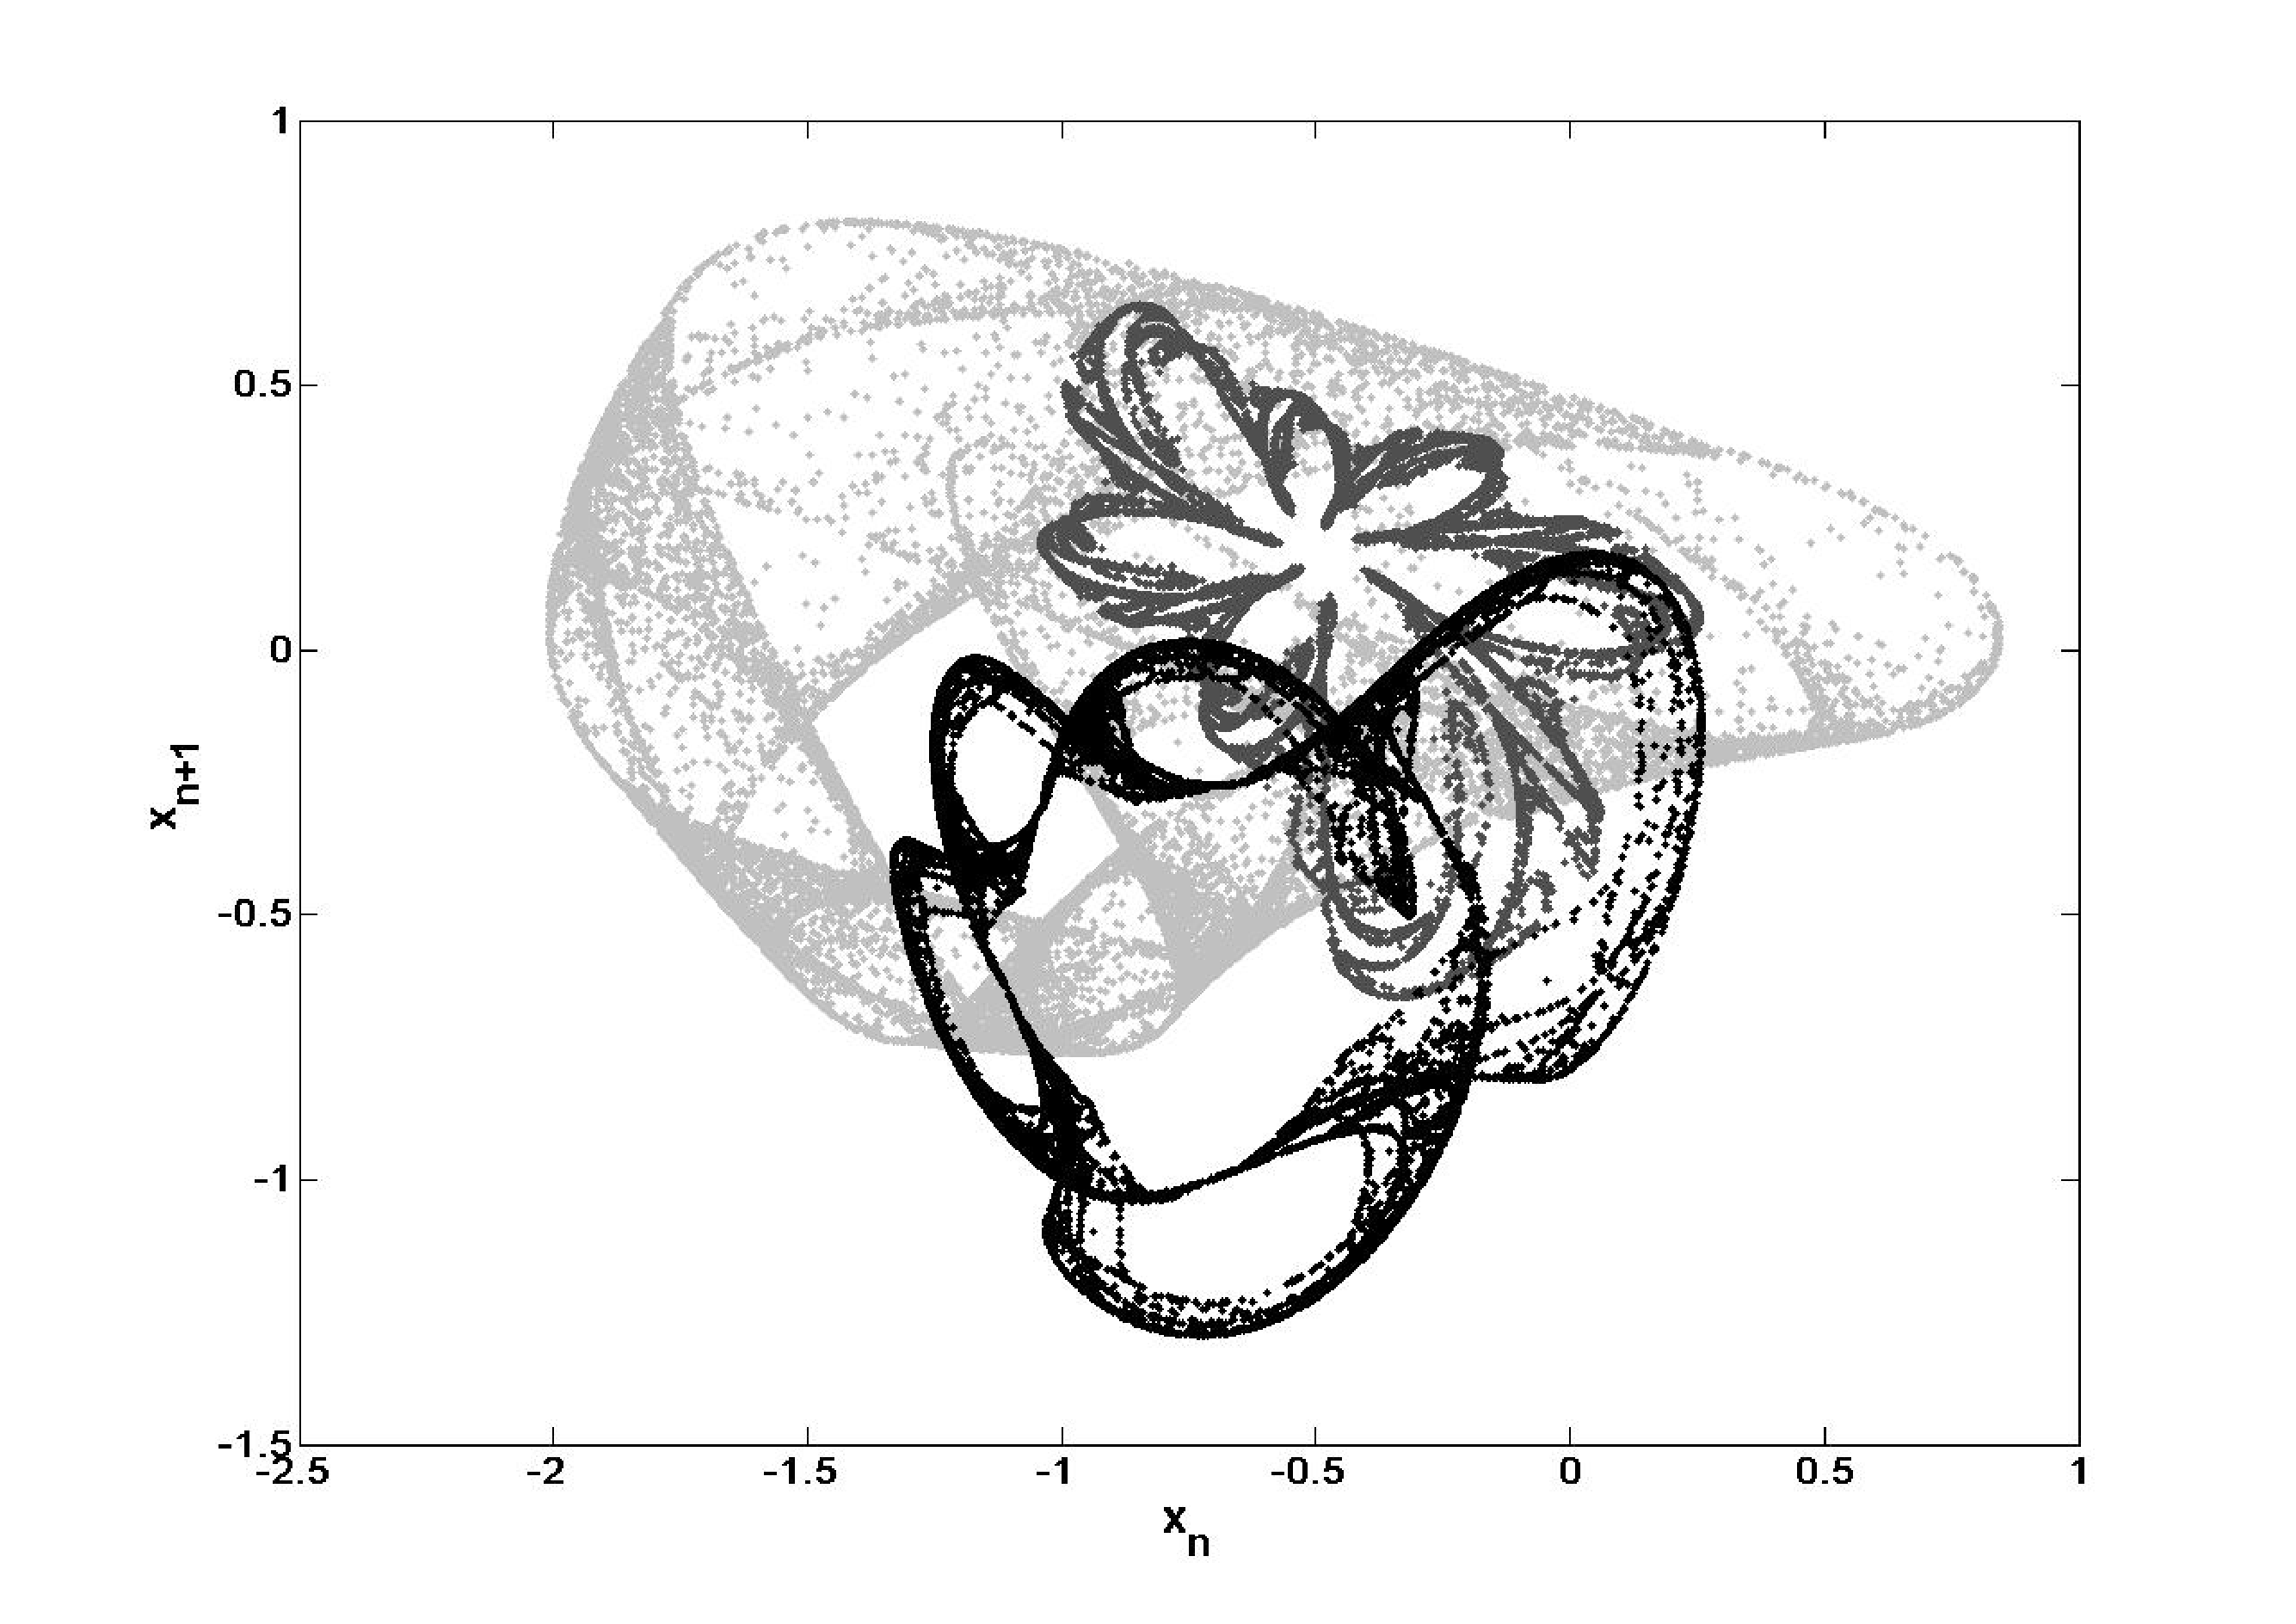
\includegraphics[width=1\columnwidth]{atractores.pdf}\\
    \caption{Atractores del sistema para tres juegos de coeficientes.}\label{fig:atractores}
\end{figure}

\subsection{Implementación}

Desde el punto de vista del esquema de codificación propuesto,
estos mapas son muy atractivos por el hecho de contar con $12$
coeficientes para generar cada atractor. Por lo tanto, las
combinaciones posibles serán $N^{12}$, en donde $N$ es la cantidad
de símblos posibles según la aritmética utilizada. En nuestro caso
empleamos una aritmética de $19$ bits expresados en complemento a
$2$ con aritmética de punto fijo, con $1$ bit de signo, $3$ bits
de parte entera y $15$ bits de parte decimal. Esta aritmética
limita y discretiza el plano $xy$ que queda delimitado por $\Delta
x=4$, $-\Delta x=-4$, $\Delta y=4$,$-\Delta y=-4$, como puede
verse en la figura \ref{fig:atractores}. Estas limitaciones al
plano de atracción tienen como consecuencia dos cuestiones a tener
en cuenta:
\begin{itemize}
    \item
        Debido a que los coeficientes se generan con la misma aritmética que las variables, nos
        encontramos con $N=2^{19}$ valores posibles para cada coeficiente,
        lo que arroja $\left(2^{19}\right)^{12}\cong4,3^{68}$ combinaciones posibles de coeficientes para generar distintos atractores.
    \item
        En cuanto a las trayectorias de los atractores sobre el plano discretizado,
        éstas se tornan periódicas debido a la discretización.
\end{itemize}


No todos los juegos de coeficientes generan atractores caóticos contenidos en el plano dado por la aritmética utilizada. Aunque esto no sería problema para la codificación/decodificación, se eligieron los coeficientes de modo que se generen atractores contenidos en el plano a modo de validación visual.

Dada la naturaleza de los mapas caóticos, un punto muy lejano a la zona de atracción puede hacer que el punto calculado para la próxima iteración diverja, por lo tanto las condiciones iniciales deben ser normalizadas antes de cambiar al mapa siguiente. Para solucionar este problema se utiliza la siguiente estrategia:
 Primero se define el plano mínimo que contiene al atractor. Para
        identificarlo se simularon los mapas mediante Quartus
        generando secuencias de salida lo suficientemente largas como para
        verificar la periodicidad. Luego se analizó este vector de datos
        con Matlab buscando los valores extremos en cada una de las
        variables: $X1_{max}$, $X1_{min}$, $Y1_{max}$, $Y1_{min}$. Estos límites delimitan al plano mínimo que contiene al atractor. La normalización dada por la ecuación \ref{eq:norm_salida} se aplica a la salida $\left(x,y\right)$ para mapear este plano minimo a todo el plano delimitado por la aritmética utilizada de dimensiones $\Delta x$, $-\Delta x$, $\Delta y$, $-\Delta y$.
Segundo, se halla el plano máximo que contiene las condiciones
iniciales que hacen que no diverja la solución sinó que genere el
atractor. Para esto se realizó un programa en Matlab que genera
los atractores desde todas las condiciones iniciales del plano
delimitado y discretizado por la aritmética utilizada, a
continuación se marcan todos los puntos que generan trayectorias
divergantes o bien convergentes a un punto fijo. Este proceso
genera la zona de condiciones iniciales factible para generar
atractores, nuevamente se identificaron los valores máximos y
mínimos del área rectangular máxima que contenga todos sus puntos
como condiciones iniciales factibles $X2_{max}$, $X2_{min}$,
$Y2_{max}$, $Y2_{min}$. La normalización dada por la ecuación
\ref{eq:norm_entrada} se aplica a la entrada de condiciones
iniciales $\left(x_{n-1},y_{n-1}\right)$ para mapear todo el plano
de dimensiones $\Delta x$, $-\Delta x$, $\Delta y$ y $-\Delta y$
al de condiciones iniciales factibles.


El problema de la existencia de puntos fijos para cierto conjunto de
coeficientes y condiciones iniciales queda salvado al perturbar
continuamente al atractor actual con valores afectados por la
información.

Se generó un circuito en VHDL con un total de $16$ juegos de
parámetros seleccionables con la palabra de entrada de $4$ bits
que se desea encriptar. Esta palabra multiplexa estos coeficientes
y alimenta un oscilador que calcula la próxima iteración de datos,
además, este circuito almacena la salida del oscilador y la
realimenta como ``condición inicial" para calcular la iteración
siguiente (Fig. \ref{fig:generador}). Como resultado de este
proceso, la salida encriptada resulta ser el oscilador actual
seleccionado por la palabra de entrada perturbado por la historia
de los mapas seleccionados por las entradas anteriores. Este
circuito de dos bloques se encarga de generar los atractores, por
lo que se lo llama ``generador de atractores".


Para la primer iteración, las condiciones iniciales son $(x;y)=(0.1;0.1)$ para cualquiera de los atractores.



\begin{figure}
    \centering
    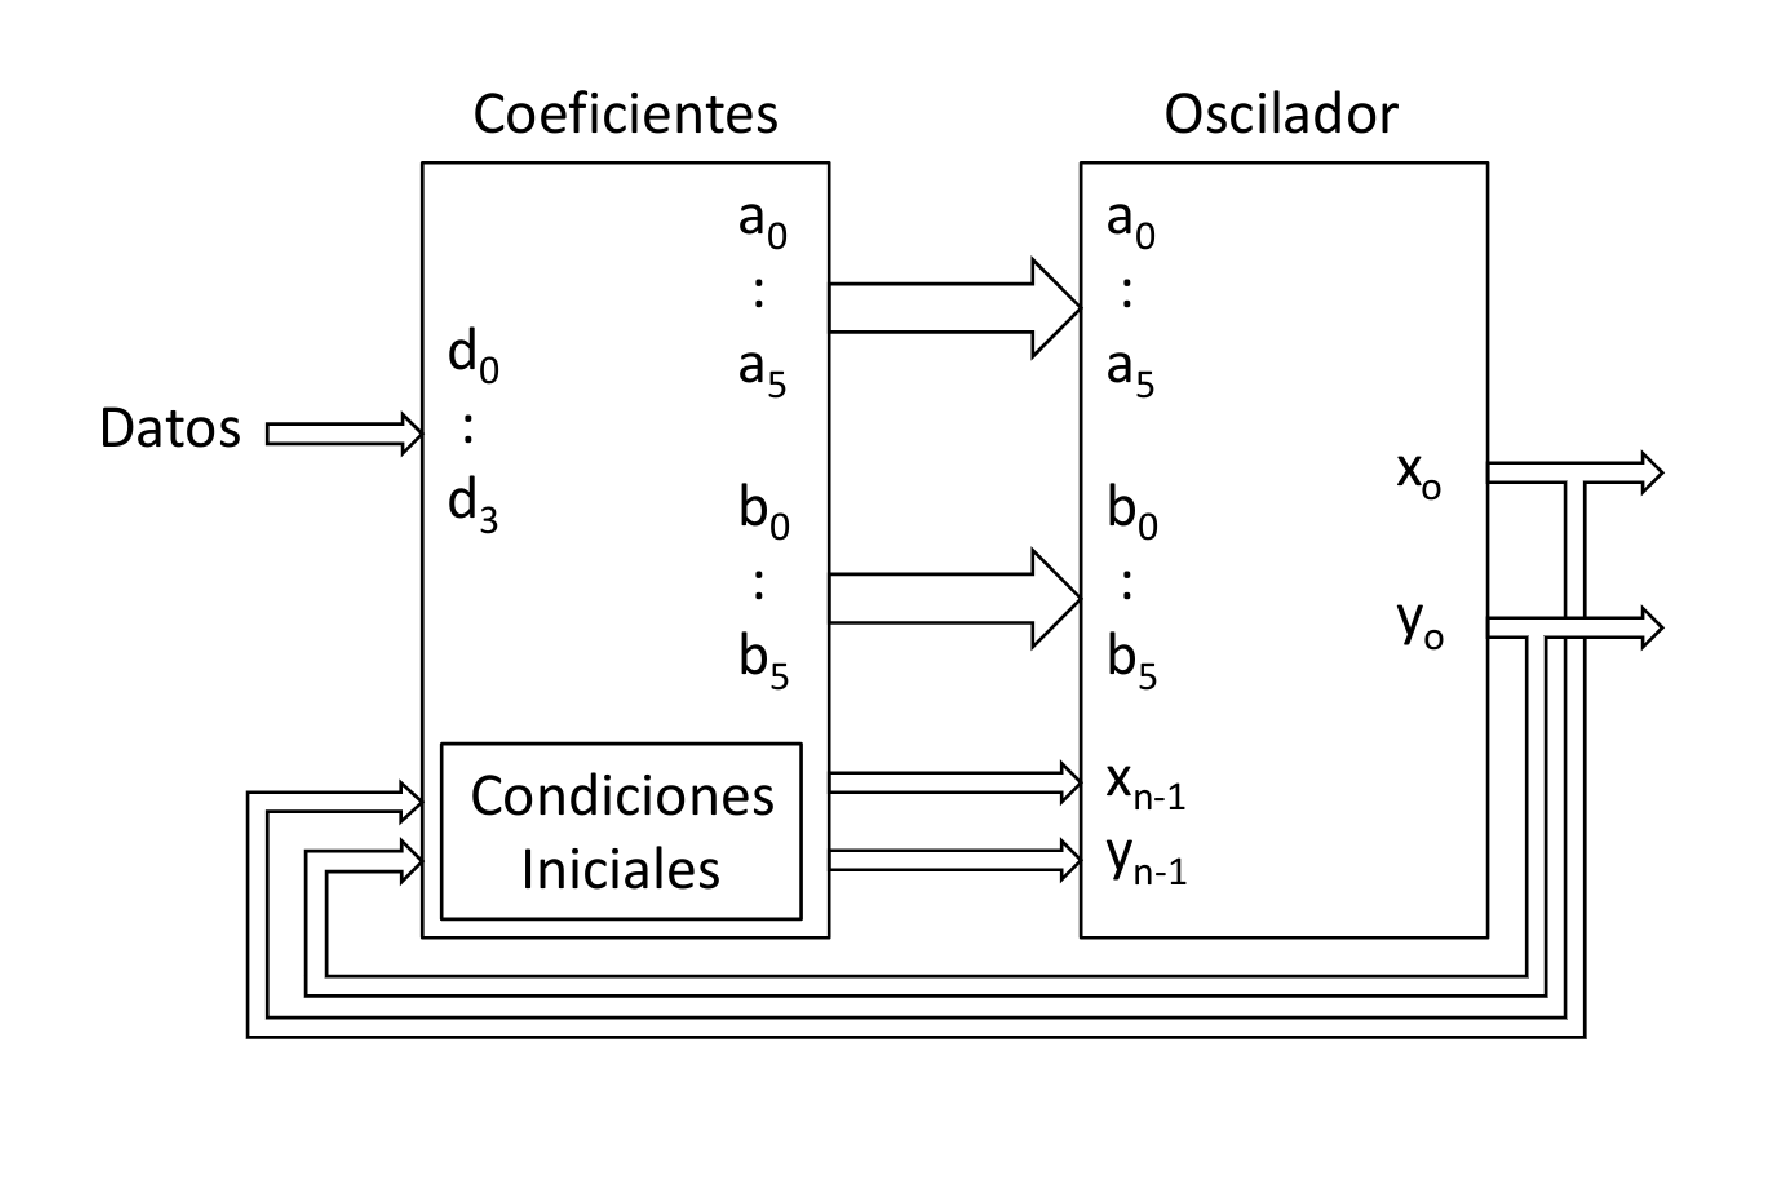
\includegraphics[width=0.7\columnwidth]{Fig1.pdf}\\
    \caption{Generador de atractores.}\label{fig:generador}
\end{figure}
{\small
\begin{eqnarray}\label{eq:norm_salida}
    x_{1norm}&=& a_{1x} x+b_{1x} \nonumber\\
    y_{1norm}&=& a_{1y} y+b_{1x} \nonumber\\
    a_{1x}&=& \frac{2\Delta x}{x1_{max}-x1_{min}} \nonumber\\
    a_{1y}&=& \frac{2\Delta y}{y1_{max}-y1_{min}} \nonumber\\
    b_{1x}&=& -\frac{x1_{max}-x1_{min}}{2} \nonumber\\
    b_{1x}&=& -\frac{y1_{max}-y1_{min}}{2}
\end{eqnarray}}
{\small
\begin{eqnarray}\label{eq:norm_entrada}
    x_{1norm}&=& a_{2x} x+b_{2x} \nonumber\\
    y_{1norm}&=& a_{2y} y+b_{2x} \nonumber\\
    a_{2x}&=& \frac{x2_{max}-x2_{min}}{2\Delta x} \nonumber\\
    a_{2y}&=& \frac{y2_{max}-y2_{min}}{2\Delta y} \nonumber\\
    b_{2x}&=& \frac{x2_{max}-x2_{min}}{2} \nonumber\\
    b_{2x}&=& \frac{y2_{max}-y2_{min}}{2}
\end{eqnarray}}

\subsubsection{Codificador}
El bloque del Codificador consiste en circuito generador y
acondicionamiento de la salida. Para codificar una palabra de
cuatro bits de entrada se generan los valores de $x$ e $y$ con el
circuito generador correspondiente a esta palabra y se los concatena en un circito posterior
formando un vector $[x:y]$ (Fig. \ref{fig:codificador}). De esta forma cada palabra de información a ser enviada será representada por la salida $xy$  del oscilador del atractor correspondiente, por lo tanto una palabra a codificar no se corresponderá con una palabra codificada, dos palabras iguales generarán dos salidas distintas.


\begin{figure}
    \centering
    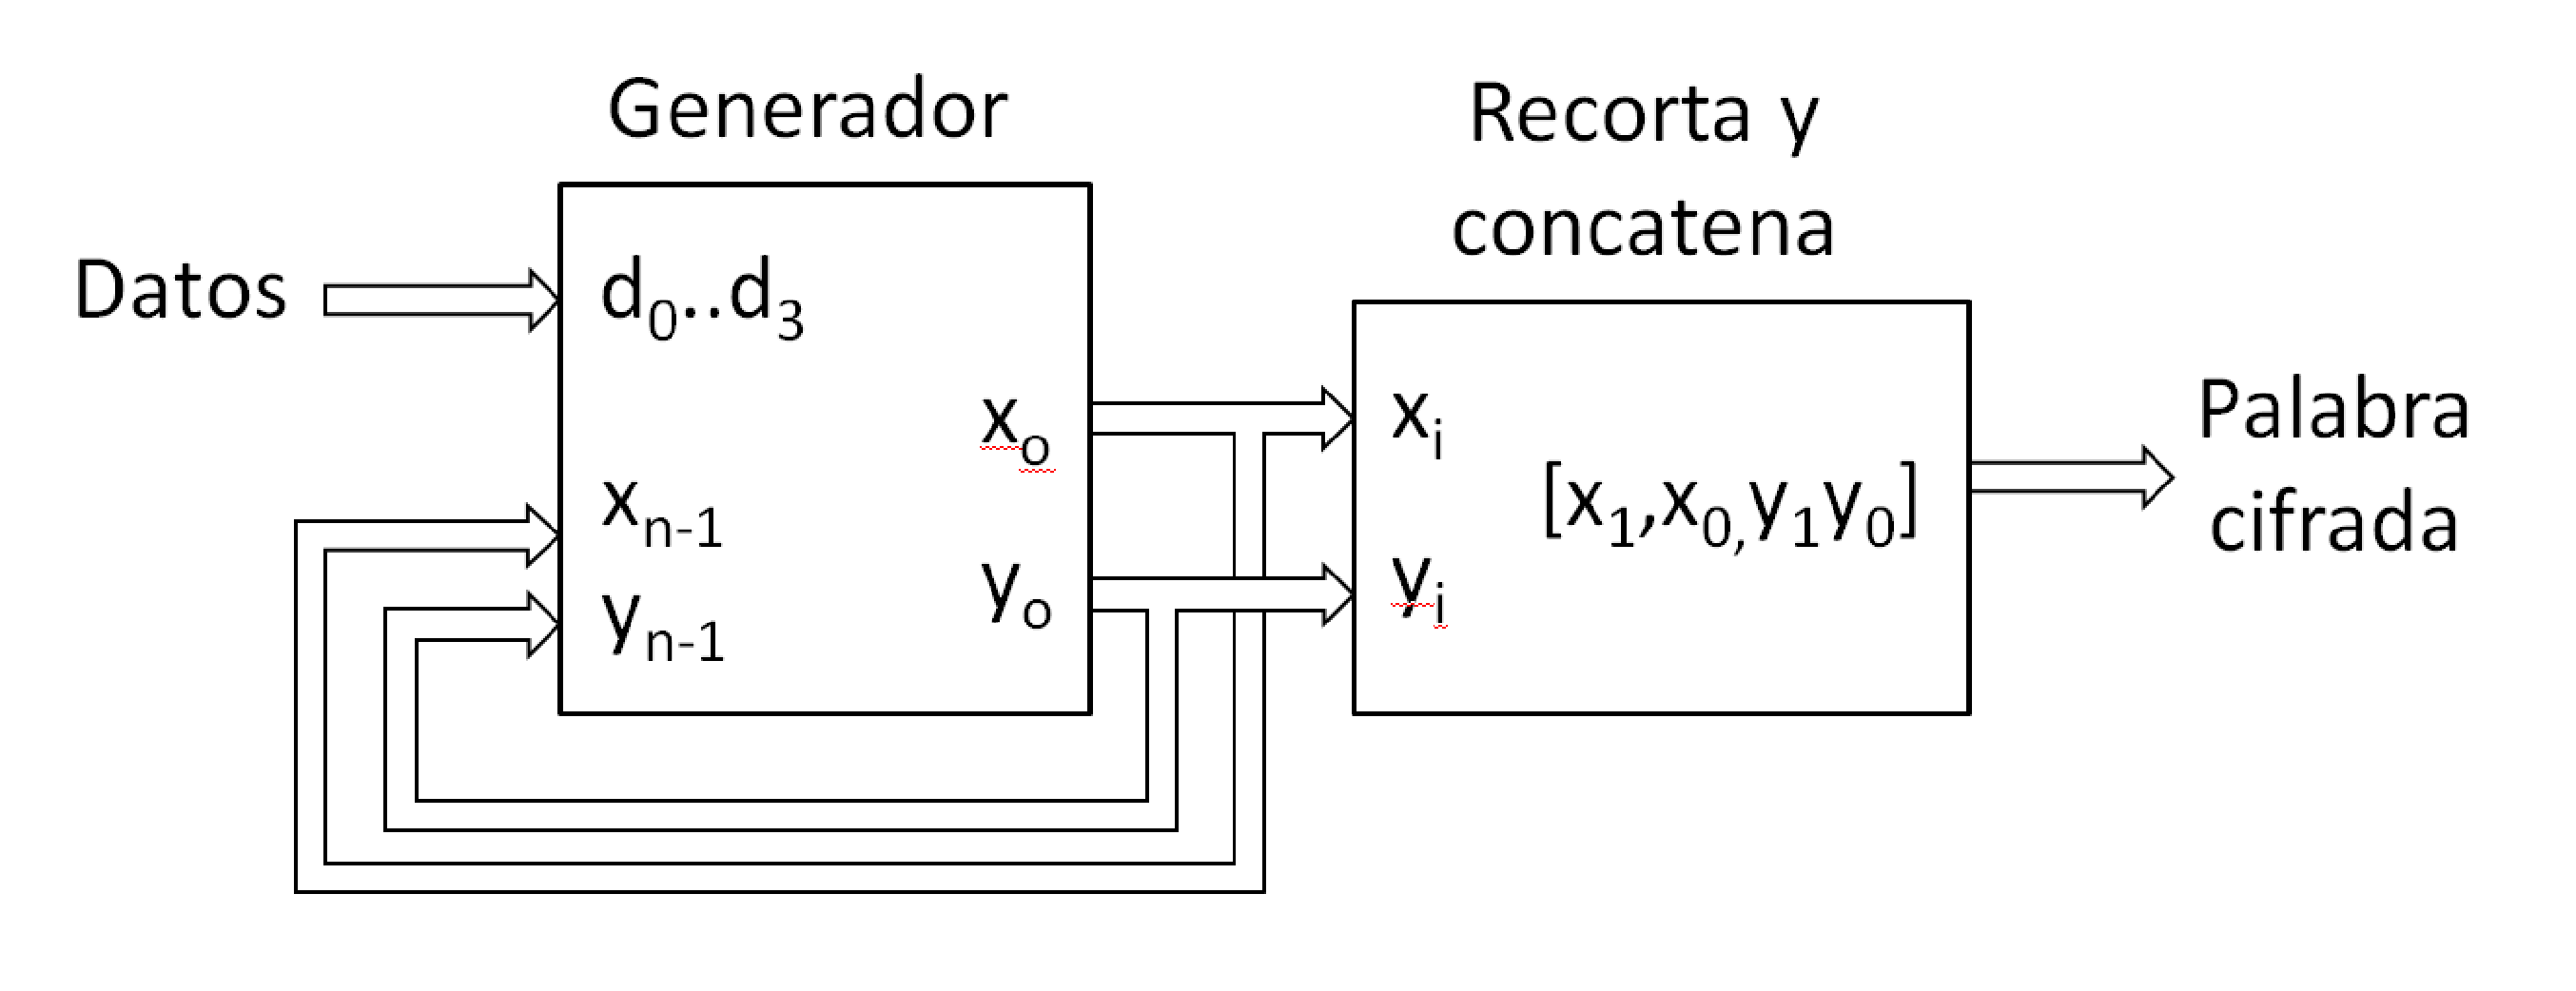
\includegraphics[width=0.8\columnwidth]{Fig2.pdf}\\
    \caption{Codificador.}\label{fig:codificador}
\end{figure}

\subsubsection{Decodificador}


Un segundo circuito generador de atractores funciona en el decodificador generando las $16$ palabras posibles para la próxima iteración. Luego, se ingresan todas estas posibles palabras
cifradas junto con la que se desea decodificar a un comparador que aplica una XOR a la palabra ingresada contra todas las palabras posibles generadas localmente para decodificarla. La
salida de este circuito es la palabra decodificada (Fig. \ref{fig:decodificador}).

\begin{figure}\
    \centering
    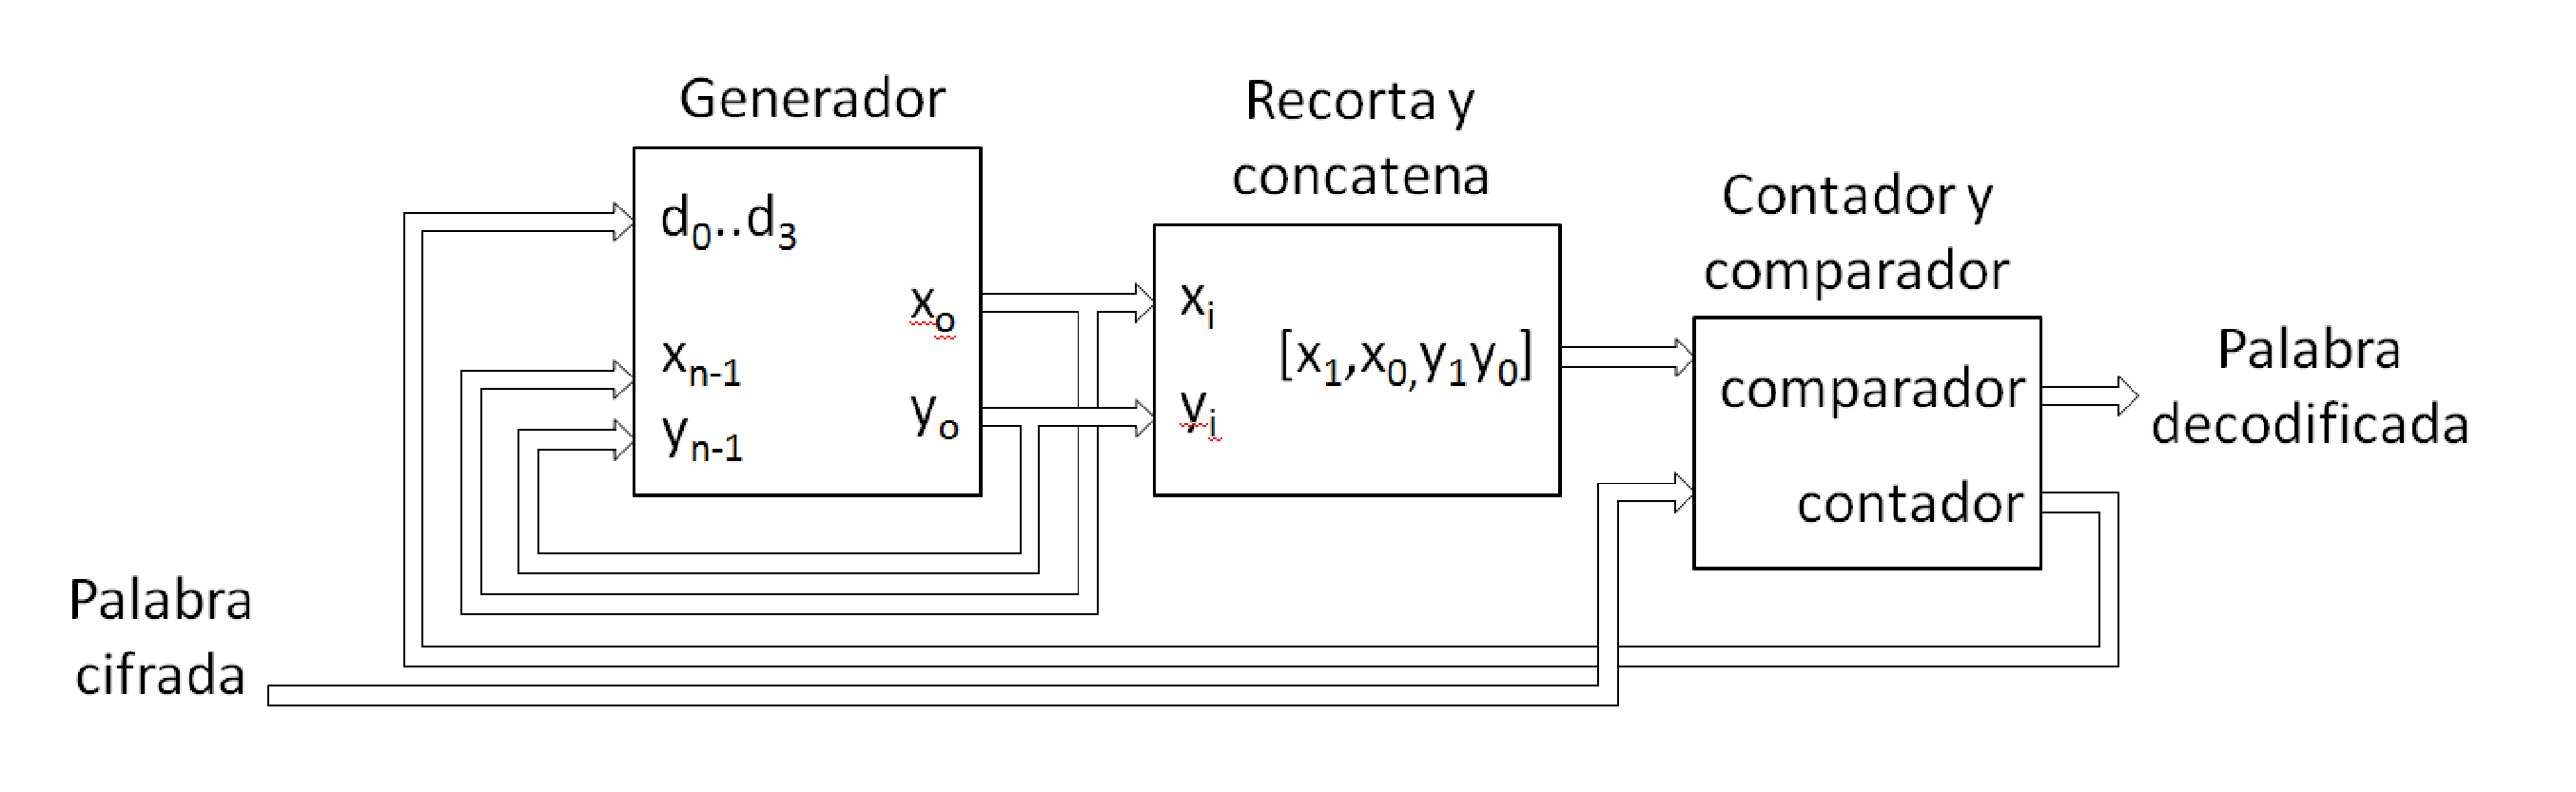
\includegraphics[width=0.8\columnwidth]{Fig3.pdf}\\
    \caption{Decodificador.}\label{fig:decodificador}
\end{figure}

\subsection{Resultados}
Se realizó un primer esquema del diseño mediante la herramienta
Quartus II v8.0 de ALTERA, para implementar el sistema en una FPGA \emph{Altera Cyclone III EP3C120}

Se obtuvieron resultados preliminares de simulaciones realizadas
mediante el programa Matlab y mediante simulaciones con el
programa Quartus de Altera, estas últimas tienen en cuenta el
empelo de la precisión finita elegida para representar los
valores.

En la Fig. \ref{senal} se pueden ver las salidas del bloque
generador para una transmisión de los datos
[1,2,3,2,3,3,1,3,1,3,1]. En este caso se mantiene el dato a enviar
durante $100$ ciclos con el objetivo de que sea visible en la
figura, en el sistema real cada oscilador codifica una palabra de
información en cada iteración. Aqui puede observarse que el
sistema cambia el atractor generado según los coeficientes que
dependen de la entrada de información a transmitir.

En cuanto al análisis de performance que presenta el sistema se
deben tener en cuenta dos aspectos:

\begin{itemize}
    \item
        La distancia mínima de la modulación codificada resultante. Esta  es
        usualmente empleada para proveer un límite de error en la región
        de piso.
    \item
        Una descripción precisa de la tasa binaria de error
        del sistema o BER (en inglés, Bit Error Rate) también es un
        parámetro muy importante, ya que da una estimación del
        comportamiento que presentara el código.
\end{itemize}


\begin{figure}
    \centering
    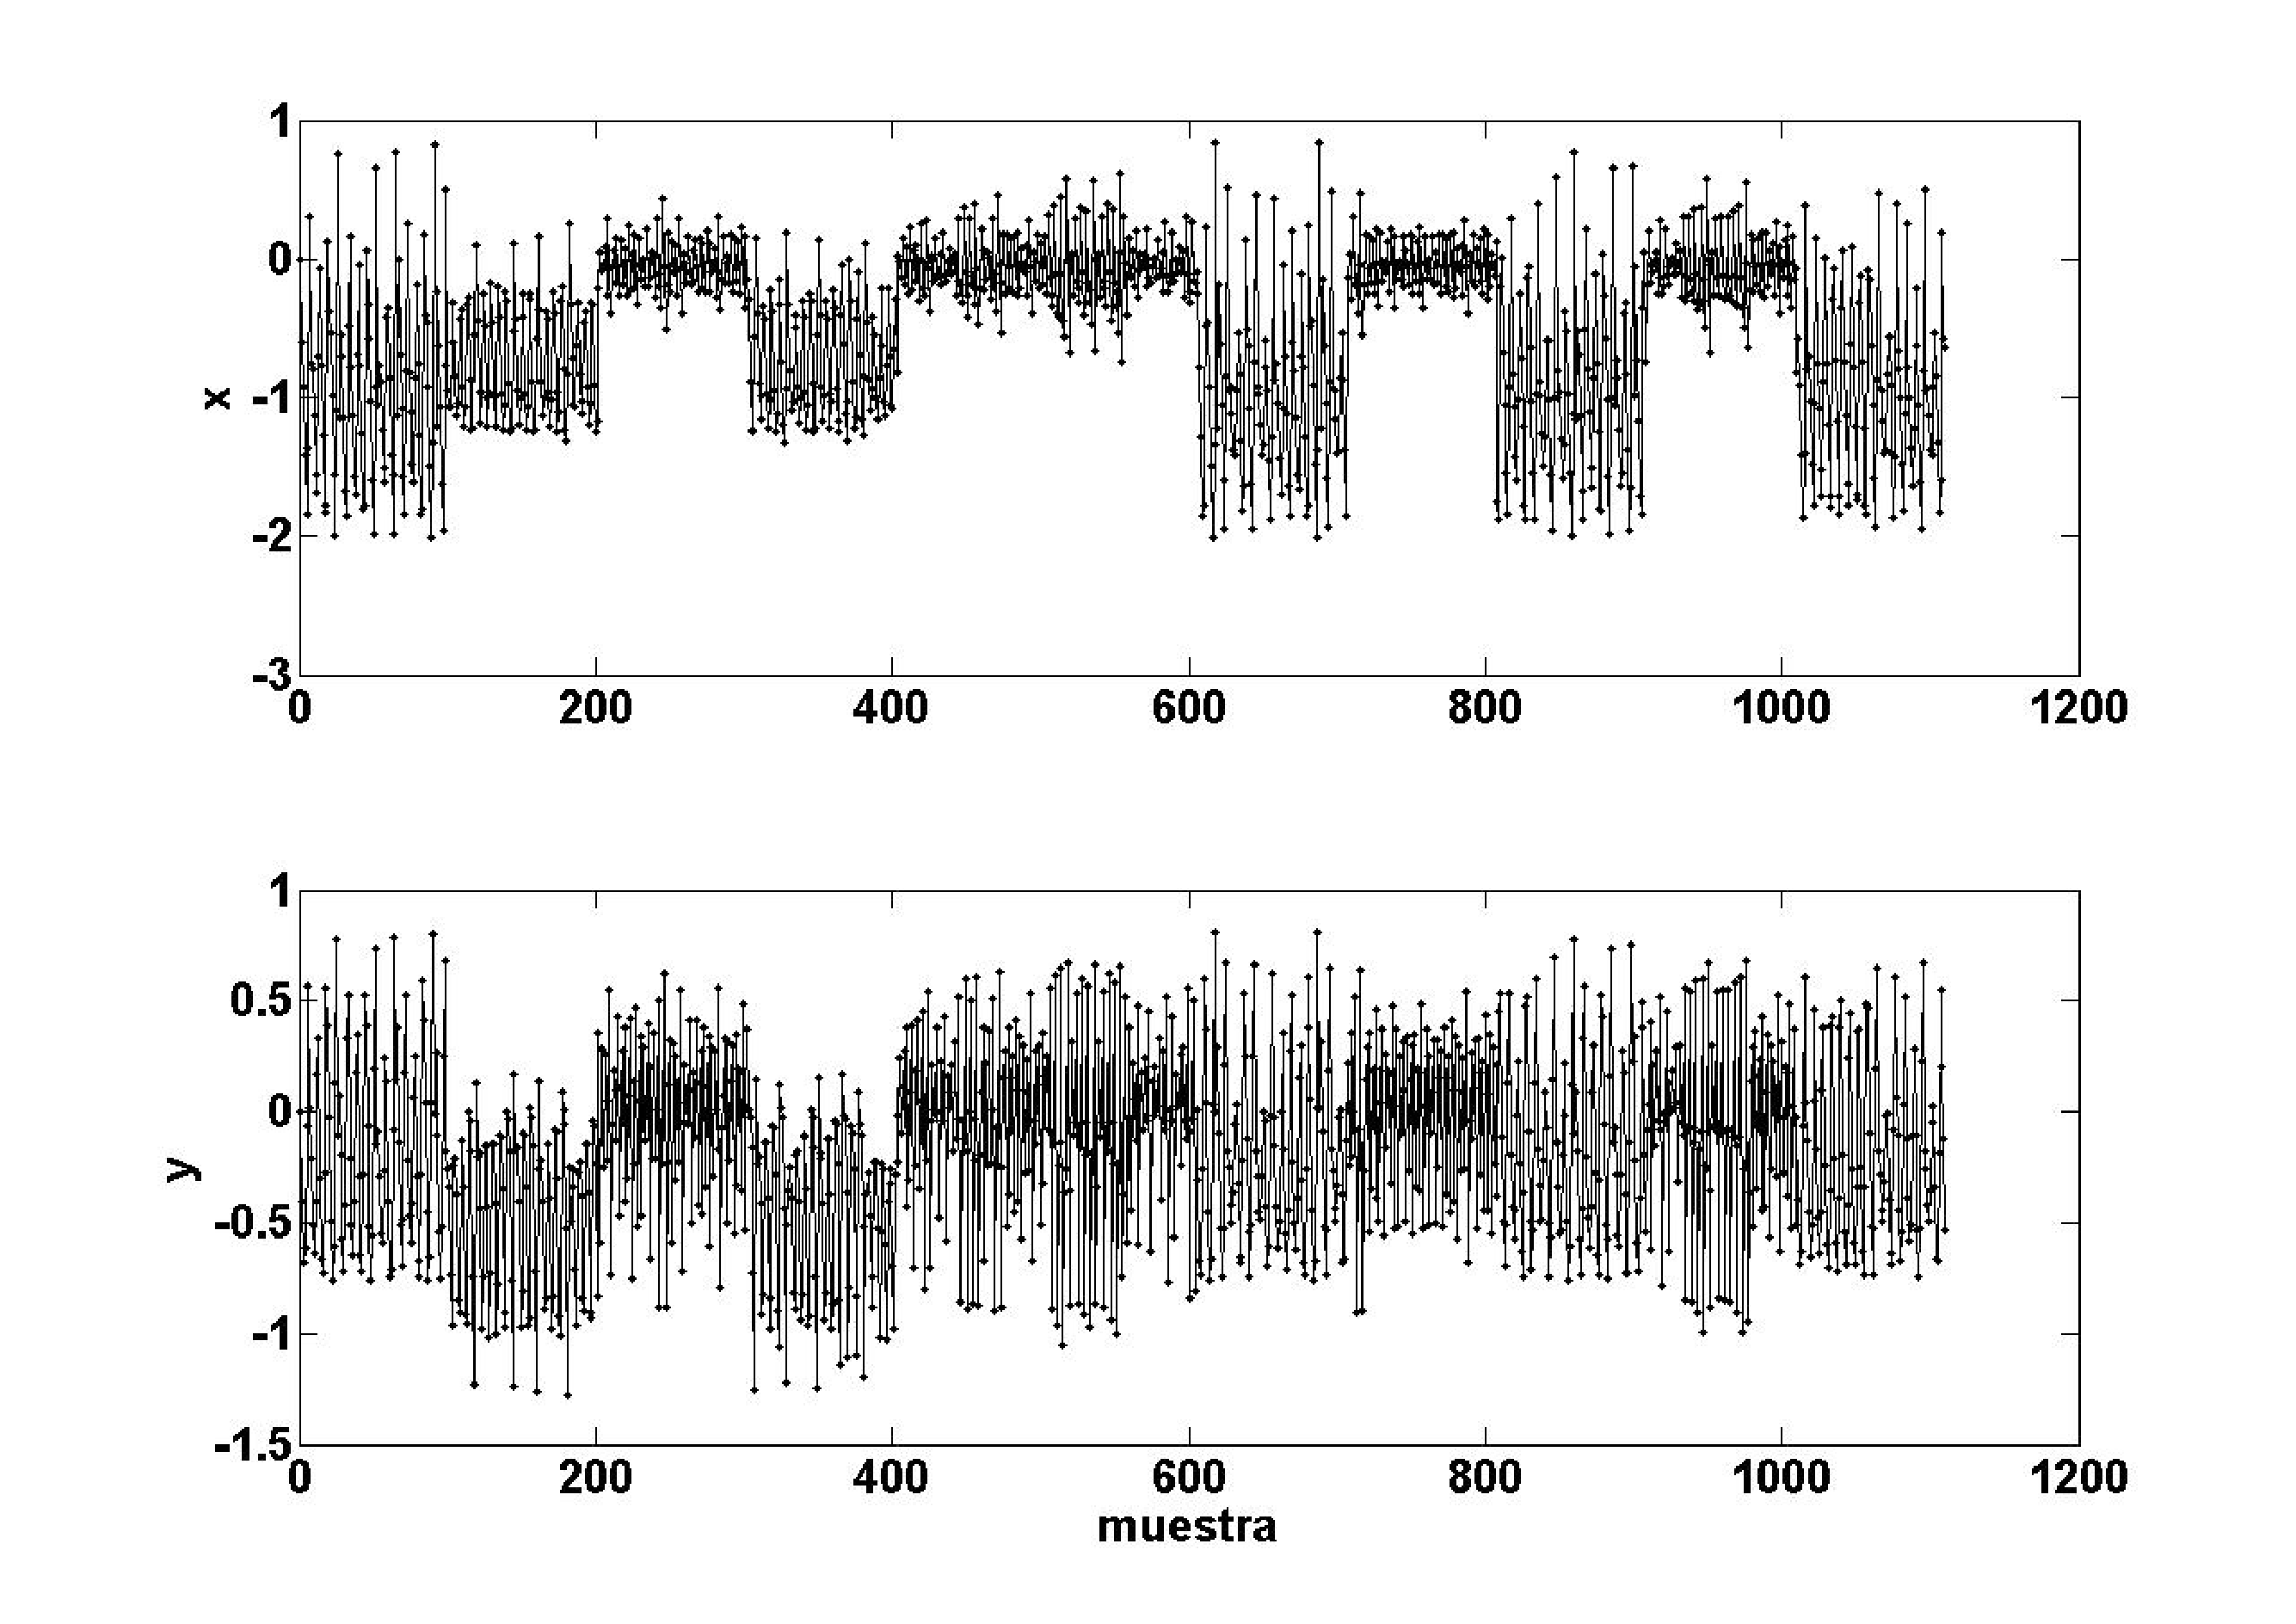
\includegraphics[width=1\columnwidth]{senalent.pdf}\\
    \caption{Señales a transmitir.}\label{senal}
\end{figure}

%\bibliography{xbibWEBjun2012_ingles}

%%%%%%%%%%%%%%%%%%%%%%%%%%%%%%%%%%%%%%%%%%%%%%%%%%%%%%%%%%%%%%%%%%%%%%%%%%%%%%%%%%%%%%%%%%%%

\section{Codificación variable en el tiempo empleando mapa caótico (póster CASE2012)}

Los posters no se si agregarlos o distribuir la información entre los demás capítulos.

En el diseño de un sistema de comunicaciones de datos inalámbrico tanto la confiabilidad de la
transmisión como el nivel de privacía son objetivos a cumplir. Han surgido últimamente técnicas de
codificación que permiten además de aumentar la confiabilidad de la transmisión frente al ruido adicionar
al sistema algún nivel de seguridad. En este trabajo se propone un esquema de codificación que cumple
con ambos objetivos. Este sistema se basa en un mapa cuadrático bidimensional cuya salida presenta un
comportamiento caótico y distintos atractores dependiendo de los coeficientes que se empleen.
Codificar significa básicamente tomar las 2k palabras binarias de k bits que se pretende codificar, y
asignarlas a algunos de los 2n vectores de n bits. Esto se realiza como una función unívoca entre los 2k y
los 2n vectores. Siendo regularmente k < n existen más vectores de n bits que los que se tienen de k bits.
Tradicionalmente el subgrupo de 2n palabras código es fijo y la elección de los vectores de n bits se realiza
empleando la menor redundancia, y maximizando la distancia o separación entre las palabras. En este
trabajo la asignación de los vectores es variable ya que a cada una de las 2k palabras a transmitir se le
asigna un juego de coeficientes que genera salida caótica del mapa. Según la palabra a transmitir el
sistema generará una salida determinada por los coeficientes y el valor inicial, esta será la palabra código
correspondiente a la palabra a enviar. De esta forma, el subespacio de palabras código va cambiando a
medida que la transmisión evoluciona.


%%%%%%%%%%%%%%%%%%%%%%%%%%%%%%%%%%%%%%%%%%%%%%%%%%%%%%%%%%%%%%%%%%%%%%%%%%%%%%%%%%%%%%%%%%%%%%%%%%

\section{Estudio del Caos en Redes Neuronales Discretas para su Implementación en Hardware (Informe Inteligencia computacional, Poster CASE2014)}

Este es bastante largo y completo, pero perdí todos los archivos junto con el disco, tengo el pdf a partir del cual voy a tener que armar el latex de nuevo.

Dentro de los sistemas complejos se encuentran los cóticos, éstos se caracterizan por tener
propiedades estocásticas similares a los de los sistemas aleatorios (en algunos casos mejores),
por ser muy sensibles a las condiciones iniciales y por ser impredecibles a mediano plazo a
pesar de contar con las ecuaciones que describen el sistema. Numerosos trabajos describen el
comportamiento caótico en redes neuronales, este trabajo presenta una detallada descripción
técnica de un caso de estudio.


%%%%%%%%%%%%%%%%%%%%%%%%%%%%%%%%%%%%%%%%%%%%%%%%%%%%%%%%%%%%%%%%%%%%%%%%%%%%%%%%%%%%%%%%%%%%

\section{\emph{RO}-based \emph{PRNG}: \emph{FPGA} implementation and stochastic analysis}

\subsection{Introduction}

The jitter and phase noises present in ring oscillators, are not
convenient in several applications of \emph{RO}s, for example in the implementation of \emph{on-chip oscillators} to generate clocks in high-speed circuits\cite{Hajimiri1999,Mandal2010,Gupta2011}. However they are the source of randomness for \emph{RO}-based \emph{PRNG} \cite{Sunar2007,Wold2009}. Furthermore \emph{RO}s can be implemented in a full-digital circuit like Field Programmable Gate Arrays (\emph{FPGA}s) as they  basically are just a string of inverters.


In \cite{Sunar2007}, Sunar et al. presented a \emph{PRNG} using
stochastic jitter by combining several \emph{RO}s. They required a
post processing of the bit stream, based on resilient functions,
to mask imperfections in the entropy source and to increase
immunity against changes in environmental conditions. The entropy of the bit stream was used to
validate the results in \cite{Sunar2007}.


Wold et al. \cite{Wold2009} proposed an enhanced version with
better random characteristics and without a post processing. They only
added an extra D flip-flop at each ring output. The
effectiveness of their proposal was tested by means of test suites available
in the open literature \cite{NIST2000,marsaglia1995,NIST2000a}.

In this paper a detailed description of a very compact hardware implementation of the \emph{RO}-based \emph{PRNG} proposed in \cite{Wold2009} is done.
In order to validate the randomness of the noise sequences generated, two quantifiers derived from the information theory are used. They define a dual entropy plane $H_{BP}$ vs $H_{hist}$.
$H_{hist}$ is a measure of the first characteristic of a \emph{PRNG} pointed in the abstract, the equiprobability among all possible values. $H_{BP}$ is a measure of the second characteristic pointed in the abstract, the independence between consecutive values. This methodology was successful to evaluate randomizing
techniques applied to chaos-based \emph{PRNG} \cite{DeMicco2008}. A comparison with other options both physical and algorithmic, proposed in the literature is made showing that, in spite of their simplicity, \emph{RO}  are good candidates as \emph{PRNG}.

Organization of the paper is as follows: section \ref{sec:hardware} describes the
hardware implementation of the \emph{RO}s mapped in
\emph{FPGA} Cyclone III. Section \ref{sec:method} shows how the normalized entropies are
determined (to keep this paper short we do not detail already
published results); \ref{sec:results} presents the
results obtained for different configurations of the same
\emph{PRNG}s proposed in \cite{Wold2009}, and the statistical comparison with other utilized \emph{PPRNG}s.
Finally we present our conclusions in Sec. \ref{sec:conclusions}.


\subsection{Hardware implementation.}

The implemented \emph{PRNG}'s consist of  several \emph{RO}s
with their outputs XORed together and sampled by a \emph{D} flip flop,
The flip flop latches the output at a selected frequency (here $100$MHz)\cite{Wold2009}.
The physical implementation is made on \emph{ALTERA}$^{\copyright}$  \emph{Cyclone} III \emph{EP3C120}
development kit with a \emph{EP3C120F780C7N} \emph{FPGA}. The design is made with \emph{Quartus}$^{\copyright}$  II 13.1 software.

\subsubsection{Chip Overview.}

\emph{FPGA}s consist of a large number of logic array blocks (\emph{LAB}s), with groups of logic elements (\emph{LE}s) for implementing sequential as well as
combinatorial circuits. In the \emph{Cyclone} III family architecture
each \emph{LAB} contains $16$ \emph{LE}s.
Basically, each \emph{LE} is a Flip Flop (\emph{FF}) with a
four-input look-up table (\emph{LUT})  (see Fig. \ref{fig:LE}). Each
\emph{LUT} can implement any function of
four variables. The \emph{FF} and the \emph{LUT} can be used together or independently, \cite{Altera}.

%=========================================
 % FIGURA
\begin{figure}
\begin{center}
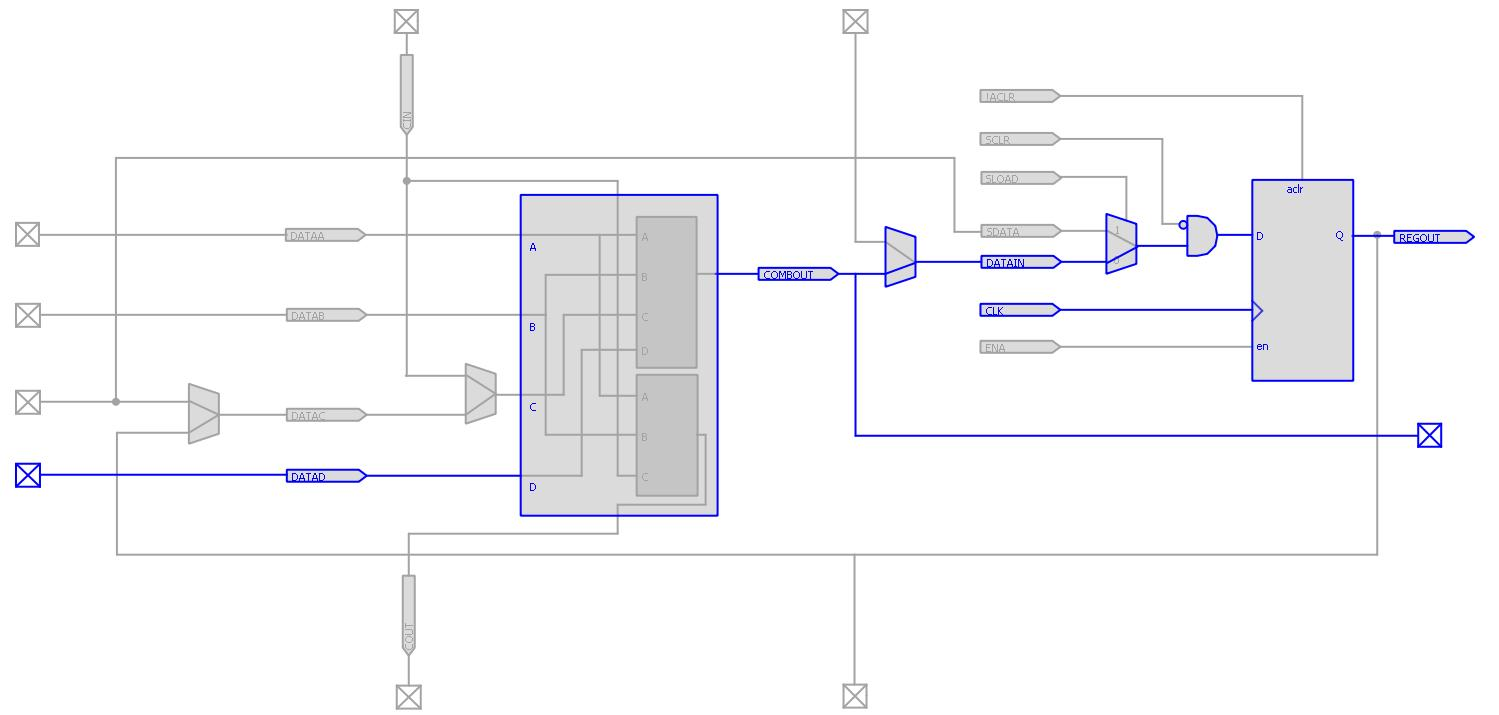
\includegraphics[ width=0.5\textwidth]{NOTenLEmasFF}
\caption{\emph{LE} implementing an inverter and a Flip Flop, Chip Planner
view.} \label{fig:LE}
\end{center}
\end{figure}
%=========================================

Usually, the logic synthesis software assigns \emph{LE}'s
resources without the designer intervention. But in the design of
\emph{RO}-based \emph{PRNG}s it is necessary to control the exact location of
each individual component for two reasons: 1) to avoid the
simplification of the inverters performed by the synthesis tool; 2) to locate
each \emph{RO} in the desired place. In \emph{Altera} the use of low-level primitives enables one to
control the hardware implementation for each \emph{cone of logic} \cite{LowLevel}. Consequently
low-level primitives and assignments are employed inside the \emph{HDL} (hardware description language) code employed in our design.

Strings of \emph{RO}s can be programmed on the chip by
instantiating the \emph{LUT}s as inverters.
In the case of \emph{RO}s it is necessary to prevent the \emph{Quartus} II synthesis engine to merge two \emph{NOT} gates in series, by using a primitive called \emph{LCELL}.
 A \emph{LCELL} always consumes one logic cell and it is not
removed from the project during logic synthesis.

These primitives allow one to break up the design into manageable parts. Each cone is as small as a \emph{LCELL} instantiation.
To create a \emph{RO}, \emph{LCELL}s are programmed as inverter-buffers. Figs. \ref{fig:RTL1ring} and \ref{fig:postMap1ring} show how this primitive is implemented by the Quartus II compiler.

\begin{figure*}
\begin{center}
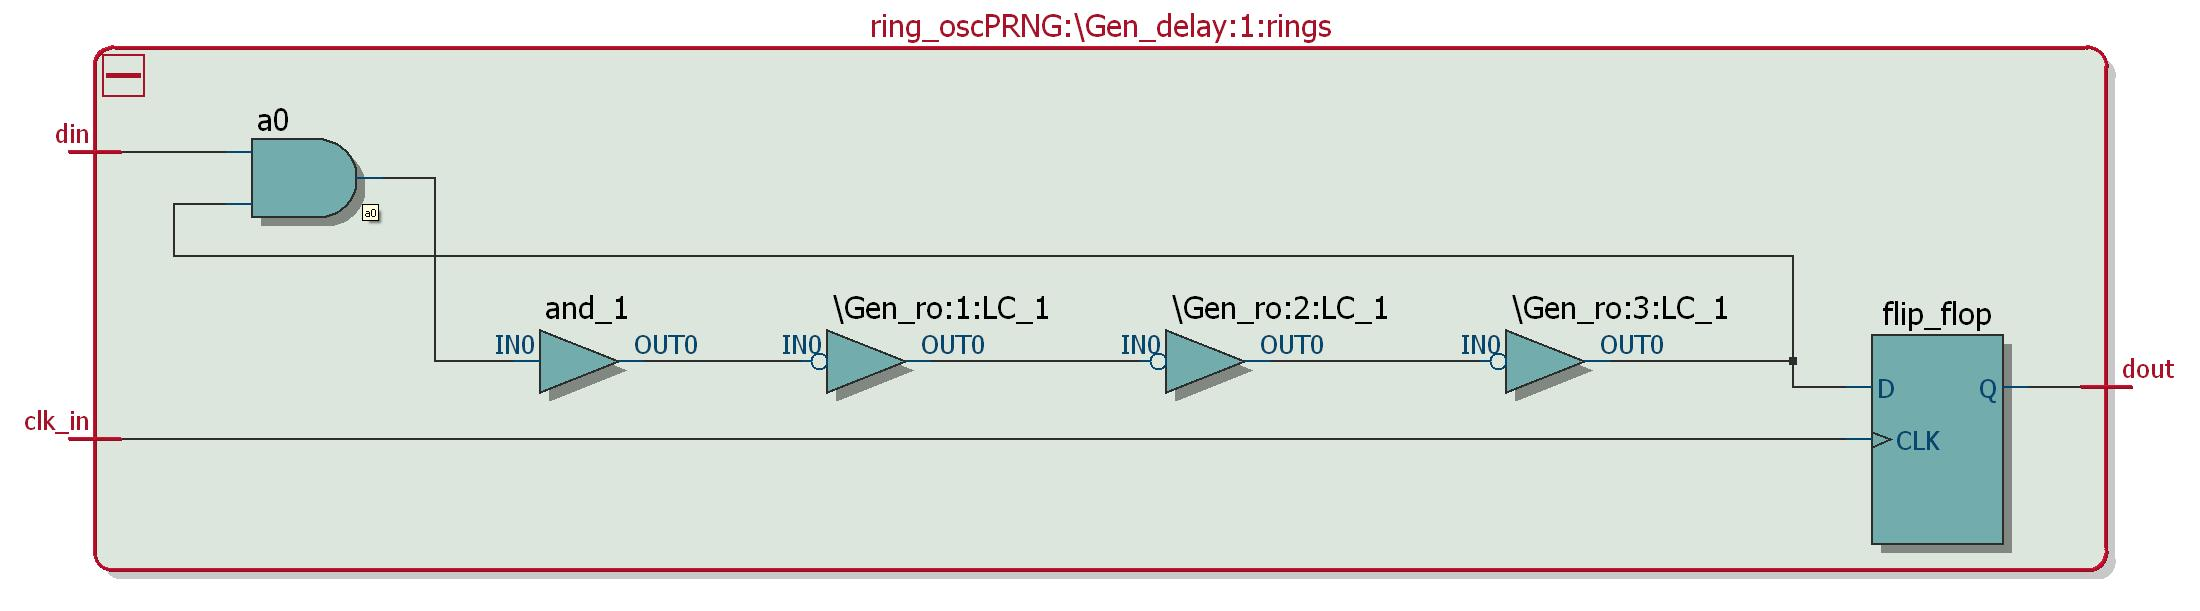
\includegraphics[ width=0.7\textwidth]{RTL_view_1ring}
\caption{RTL view one ring with $3$ inverters.}
\label{fig:RTL1ring}
\end{center}
\end{figure*}

%=========================================
 % FIGURA
\begin{figure*}
\begin{center}
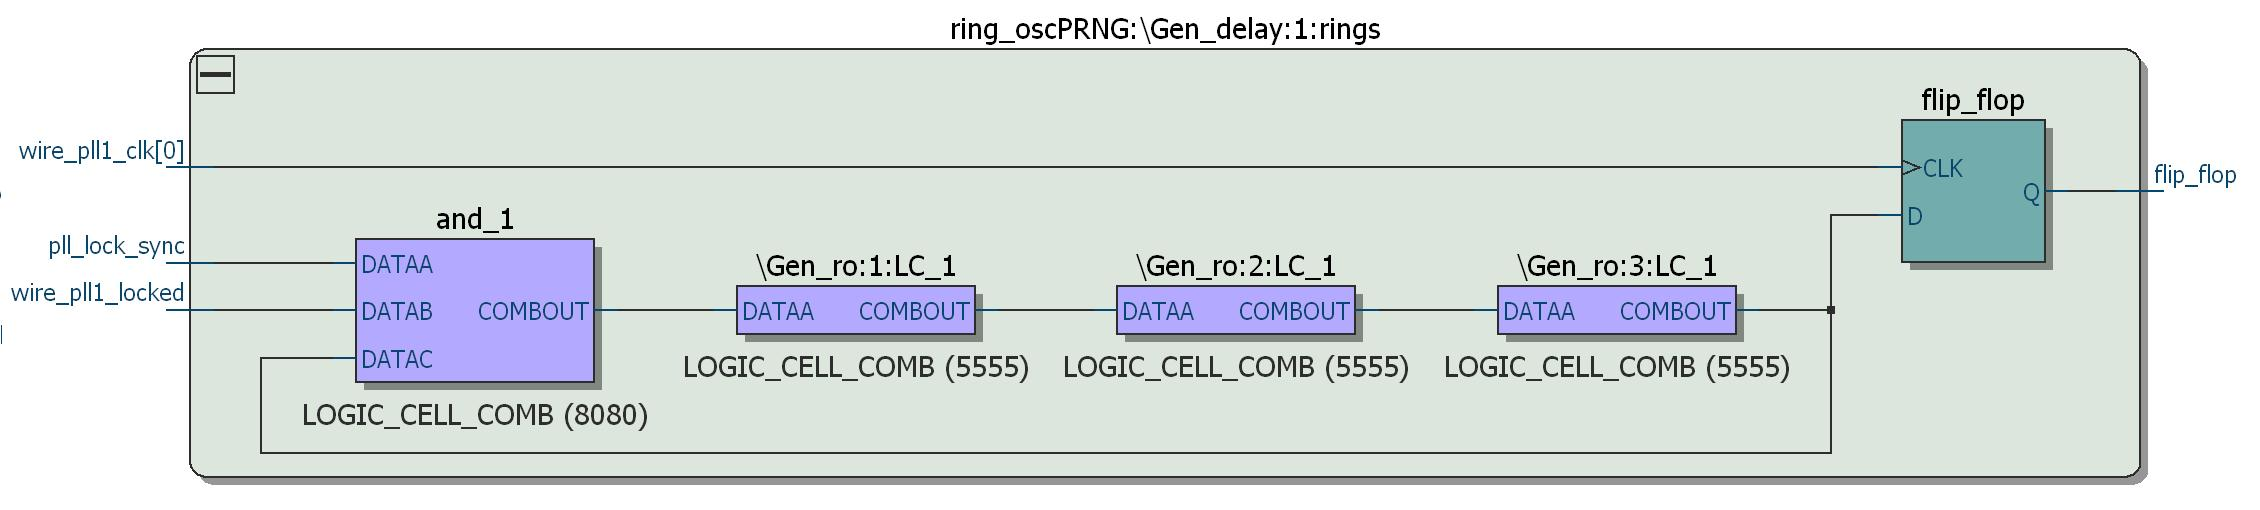
\includegraphics[ width=0.7\textwidth]{tech_map_viewer_post_mapping}
\caption{Technology map viewer (post mapping), one ring with $3$
inverters.} \label{fig:postMap1ring}
\end{center}
\end{figure*}
%=========================================

Furthermore, to avoid the synthesis tool to optimize removing the redundant buffers away,
the \empty{Ignore \emph{LCELL} Buffers} must be set in
\emph{OFF} in the \emph{More Analysis \& Synthesis
Settings} dialog box. Also \emph{Remove Redundant Logic Cells}
must be set to \emph{OFF}.

In order to place each \emph{RO} at a desired position, it
must be assigned to a previously defined \emph{LogicLock region}. In this way the \emph{fitter} will keep all the elements of each ring inside the same region,
\cite{LogicLockRegions}. The process of mapping all the elements to a particular location on the chip
(\emph{LogicLock} region) is achieved by the \emph{Assignment
Editor} tool, that also allows one to verify
that the placements are actually still there, after the  \emph{Synthesis} and \emph{Place \& Route} processes.

Fig. \ref{fig:fpgaplan} shows the $50$ \emph{LogicLock} regions used in this paper as they are
established in the die. One \emph{RO} is assigned to each region.
Regions are spread over the die for a future analysis of location importance. Each region has  $16$ \emph{LAB}s, to allow us to increase the number of inverters of each ring, an issue to be considered in future work.


%=========================================
 % FIGURA
\begin{figure*}
\begin{center}
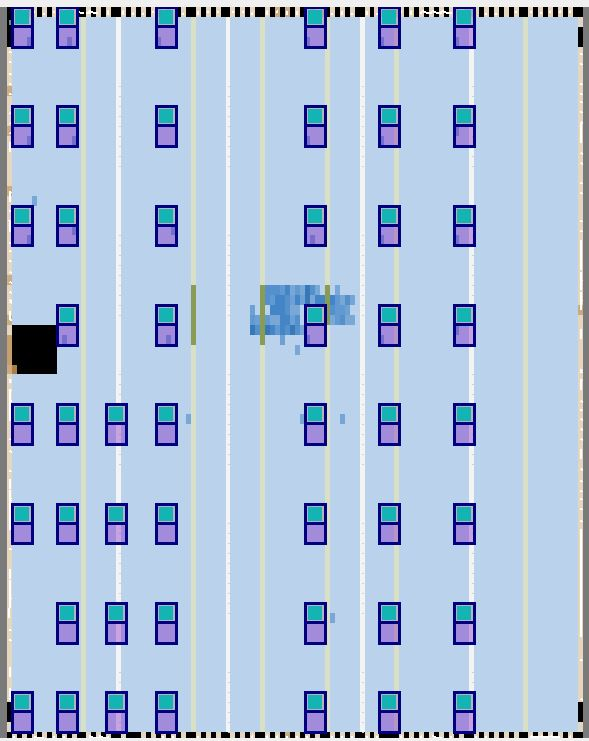
\includegraphics[ width=0.5\textwidth]{fpgaplan}
\caption{\emph{Chip Planner} view \emph{LogicLock} regions.}
\label{fig:fpgaplan}
\end{center}
\end{figure*}
%=========================================

 $3-$inverters, employed in a \emph{RO} and the \emph{FF} were all mapped onto a  \emph{LE} each, meaning that the block
utilization is $4$ of $16$ \emph{LE}s for any \emph{LAB}.


Fig. \ref{fig:LE} displays a single \emph{LE}, there an inverter is
implemented in the \emph{LUT} and it can be seen the exact
\emph{LUT} input that is used. Also the output \emph{FF} of
the ring is mapped there.


There are many factors that determine the frequency of each
\emph{RO}, and contributes to the unpredictability of the output:
\begin{enumerate}
\item Placement within the \emph{LAB}: different placements between rings could result in timing differences.
\item Connections: even having exactly
identical placement of the \emph{LUT}s with respect to each other
in a given ring, it is not possible to have exactly the same
\emph{routing resource usage} in the connections. A small difference in
\emph{routing resource usage} could affect the ring delay.
\item Input selection:  the \emph{fitter} will choose which
\emph{LUT} input is utilized during the routing stage. But the delay through the \emph{LUT}
depends on which of the four inputs is used and consequently the rings could
also have different delays.
\item Neighborhood: even if the design locks down all the placement and routing of a
section  and everything is
physically locked, the timing can change by a few picoseconds
depending on what is placed and routed around the ring.\end{enumerate}
%
In Fig. \ref{fig:RTL3rings} (RTL view) it is shown a \emph{PRNG} using $3$ \emph{RO}s
followed by a XOR gate.

% FIGURA
\begin{figure}
\begin{center}
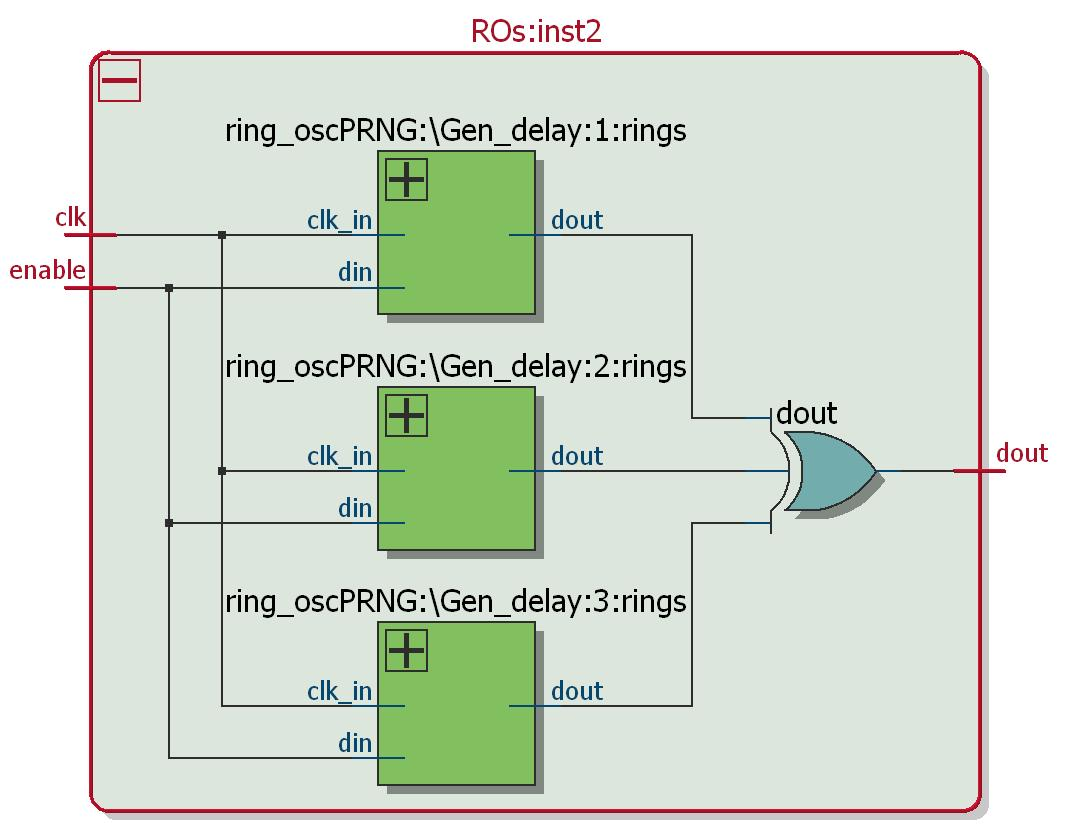
\includegraphics[ width=0.5\textwidth]{RTL_view_3ROs}
\caption{\emph{RTL} view of \emph{PRNG} with $3$ \emph{RO}s.}
\label{fig:RTL3rings}
\end{center}
\end{figure}

%=========================================

Finally, Table \ref{compilation} shows the compilation report of the \emph{PRNG}  using $15$ \emph{RO}s each with $3$ inverters.


%=========================================
\begin{table}
\begin{center}
\begin{tabular}{| l | c  c | }
 \hline
 
\footnotesize{Total logic elements} & $847/119,088$ & $ ( < 1 \%)$\\

 \hline
 
\footnotesize{Total combinational functions} &  $629/119,088$ & $( < 1 \%)$ \\

 \hline
 
\footnotesize{Dedicated logic registers} & $617/119,088$ & $( < 1 \%)$ \\

 \hline
 
\footnotesize{Total registers} &  $617$ &   \\

 \hline
 
\footnotesize{Total memory bits} &  $131,072/3,981,312$ & $( 3 \%)$ \\

 \hline
 
\end{tabular}
\end{center}
\caption{Compilation Report, \emph{RO}-based \emph{PRNG} using $15$ \emph{RO}s and $3$ inverters each.}
\label{compilation}

\end{table}




%==========================================



\subsection{Quantifiers}
\label{sec:method}
Let $X=\{x_i, i=1,...,N\}$ be a length $N$  output of a given
symbolic source with alphabet $\mathcal{A}=\{a_i,i=1,...M\}$. Each
element of $X$ is  $x_i \in \mathcal{A}$. In the case of \emph{RO}
the alphabet is binary consisting of two symbols
$\mathcal{A}=\{0,1\}$. The output is converted into words of $n$
elements. In our case $n=6$. It means we work with a time series
$Y=\{y_i,i=1,...K$ with $K=N/6\}$  of natural numbers $y_i\in [0,2^6-1]$.

The obvious \emph{PDF} (probability density function) to characterize $Y$ is the normalized histogram of the $K$
words $Y$; let us call it  $PDF_{hist}$. Its normalized Shannon
entropy $H_{hist}$ is given by:
\begin{equation}
\label{eq:entropia}
H_{hist}=\frac{\sum_{i=1}^{K}{p_i~log~p_i}}{logK}
\end{equation}

We call this \emph{PDF}  \emph{non-causal} because it does not
change if we permute the time order of the words, and consequently
can not detect any causal connection between consecutive words. The normalized entropy
$H_{hist}$ quantifies the equiprobability of the words among all
possible values. For a \emph{PRNG} its ideal value is
$H_{hist}=1$.

To quantify statistical independence between consecutive words we
use a \emph{causal} \emph{PDF}, proposed by Bandt \& Pompe
\cite{Pompe2002}. This \emph{PDF} is obtained by assigning
ordering patterns to overlapped segments, of length $D$, of the
time series trajectory. The process is as follows: 1) group $D$
consecutive words $\{y_i,y_{i+1},...,y_{i+D}\}$ (let us stress that in our case each
$y_i$ is a natural number $\in[0,63]$). The ordering of the $D$
values inside each group is compared with the order of numbers
$\{1,2,...,D\}$. There exist $D!$ possible permutations of $D$ elements.
Each permutation is called an \emph{ordering pattern}
\cite{Amigo2006} and is labelled with a permutation number
$\pi=1,...,D!$. The normalized histogram of $\pi_i$'s is called
the Bandt \& Pompe \emph{PDF}, $PDF_{BP}$. The normalized Shannon entropy of
this $PDF_{BP}$ is $H_{BP}$ where the subscript $BP$ means ``Bandt
and Pompe".

In case two values of $y_i$ inside the same group are identical,
it is considered that the first one is lower than the last one in
order to obtain an unique result. For \emph{PRNG}s this procedure
does not produce significant changes in  $PDF_{BP}$.

The  Bandt \& Pompe procedure has the advantages of being: 1) simpler and
fast to calculate than block entropies, 2)
robust in presence of noise, and 3) invariant to lineal
monotonous transformations. It is applicable not only to
\emph{PRNG}s but also to any weak stationary process (it means for $k=D$,
the probability that $x_t < x_{t+k}$ does not depend on the
particular $t$ \cite{Pompe2002}). The causality property of $PDF_{BP}$
makes the quantifiers based on this \emph{PDF} to discriminate
between deterministic and stochastic systems \cite{Rosso2007B}.

Bandt and Pompe suggested $3\leq D \leq7$. $D=6$ is adopted
in this work.

A full discussion about the convenience of using different quantifiers
to measure a given \emph{PDF}is out of the scope of this work.
Nevertheless reliable bibliographic sources
do exist \cite{Wackerbauer1994,Lopez1995,Rosso2007A,DeMicco2008,Rosso2009,Martin2006,Rosso2012}.

In this paper we adopt plane $H_{BP}$ vs $H_{hist}$ \cite{DeMicco2008}  to represent each \emph{PRNG}. A higher
value in any of the entropies, $H_{BP}$ and $H_{hist}$, implies an
increase in the uniformity of the involved \emph{PDF}'s. The point
$(1,1)$ represents the ideal point for a \emph{PRNG} with uniform histogram and
uniform distribution of ordering patterns.

\subsection{Results}
\label{sec:results}
%

The  \emph{Embedded Logic Analyzer} tool is utilized for collecting the random sequences generated.
It constitutes a \emph{system-level debugging tool}, provided by $Altera$  \cite{QUARTUS}, that captures and storages the real-time signal behavior and allows one to observe interactions between hardware and software in system designs. After acquiring
the data and  save them into a \emph{SignalTap} II file, they can be
analyzed or viewed as a waveform. With this procedure nor extra jitter neither distortion are introduced in the measured signal from the data acquisition chain.


In the case of \emph{RO} based \emph{PRNG}
data files with $917504$ bits each were generated for each \emph{RO} based \emph{PRNG}.
We consider sets of $N_{RO}$ rings, each with $3$ inverters; $N_{RO}=2$, $3$, $4$, $5$, $6$, $7$, $15$, $25$ and $50$.

Data from $SignalTap$ were  processed using \emph{Matlab}$^\copyright$. Binary data were grouped in $6$-bits words without
superposition, so files with $152917$ data each were generated. Quantifiers described in section \ref{sec:method} were calculated
for all generated files.

We also evaluated other known noises generators to compare their quality with that of  the \emph{RO}-based \emph{PRNG}.
The noises analyzed are:


\begin{itemize}
  \item Mersenne Twister pseudo-random number generator, \cite{Matsumoto1998}.
  \item Two algorithms employed for generate random data by Matlab (Multiplicative Congruential method) \cite{Matlab} and Excel \cite{McLeod1985}.
  \item Two \emph{physical noises}: radioactive decay noise \cite{Walker2001} and atmospheric noise \cite{Haahr}.
  Data files for these noises are available from the referred \emph{websites}.
  \item Two chaotic map $M^1$ and their iterated versions $M^2$ to $M^8$ \cite{DeMicco2008} for the logistic map (\emph{LOGISTIC}) and the \emph{three way Bernoulli map} (\emph{TWBM}).
\end{itemize}

Fig. \ref{fig:HBPvsHhis_all} shows the results in the dual entropy plane $H_{BP}$ vs $H_{hist}$ for all these noises.
It can be seen that the \emph{physical noises}, the algorithmic \emph{Mersenne Twister}, and the \emph{PRNG}s used in \emph{Matlab} $^\copyright$(\emph{rand} function) and \emph{Excel}$^\copyright$ (\emph{RAND} function), have the  maximum value for $H_{BP}$, indicating that all the ordering patterns appear almost the same number of times. However these five noises present very different behavior with respect the $H_{hist}$ quantifier. The \emph{radioactive decay} is the worst, with a value of $H_{hist}$ about $0.5$ indicating that this sequence does not exhibit all possible values in the same proportion. In Fig. \ref{fig:HBPvsHhis_all} the numbers next to each marker for the chaotic sequences, indicate the number of iteration. The iterated maps have higher $H_{BP}$ because of their mixing property \cite{DeMicco2008}.


 % FIGURA
\begin{figure*}
\begin{center}
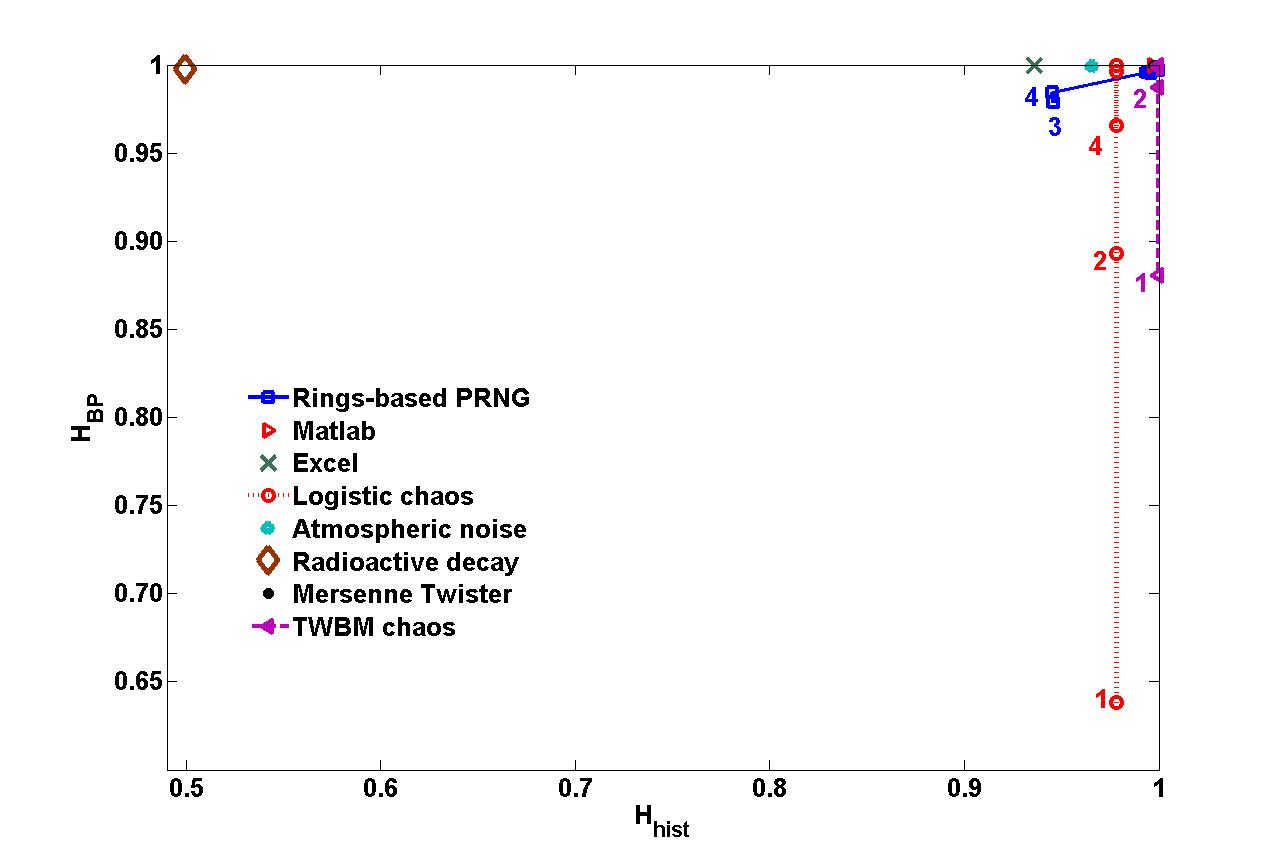
\includegraphics[ width=0.8\textwidth]{HhistvsHBP_t}
\caption{$H_{BP}$ vs $H_{hist}$ plane for several noises, numbers next to each square indicate the quantity of \emph{RO}s
used in the \emph{RO} based \emph{PRNG}. Numbers next to each point in the  chaotic sequences labeled \emph{Logistic}
and \emph{TWBM} indicate the number of iteration of the chaotic map (see the text for details).}
\label{fig:HBPvsHhis_all}
\end{center}
\end{figure*}
%=========================================

In the case of the \emph{RO}-based \emph{PRNG} sequences, numbers next to each square indicate the quantity of \emph{RO}s employed in that \emph{PRNG} (let us stress that the number of inverters is fixed to $3$). The dual entropy plane shows that  an increase in the number of \emph{RO}s improves both $H_{BP}$ and $H_{hist}$.

Fig. \ref{HhistvsHBP_zoom} is a zoom of Fig. \ref{fig:HBPvsHhis_all}  around the ideal point $(1,1)$.


%=========================================
 % FIGURA
\begin{figure*}
\begin{center}
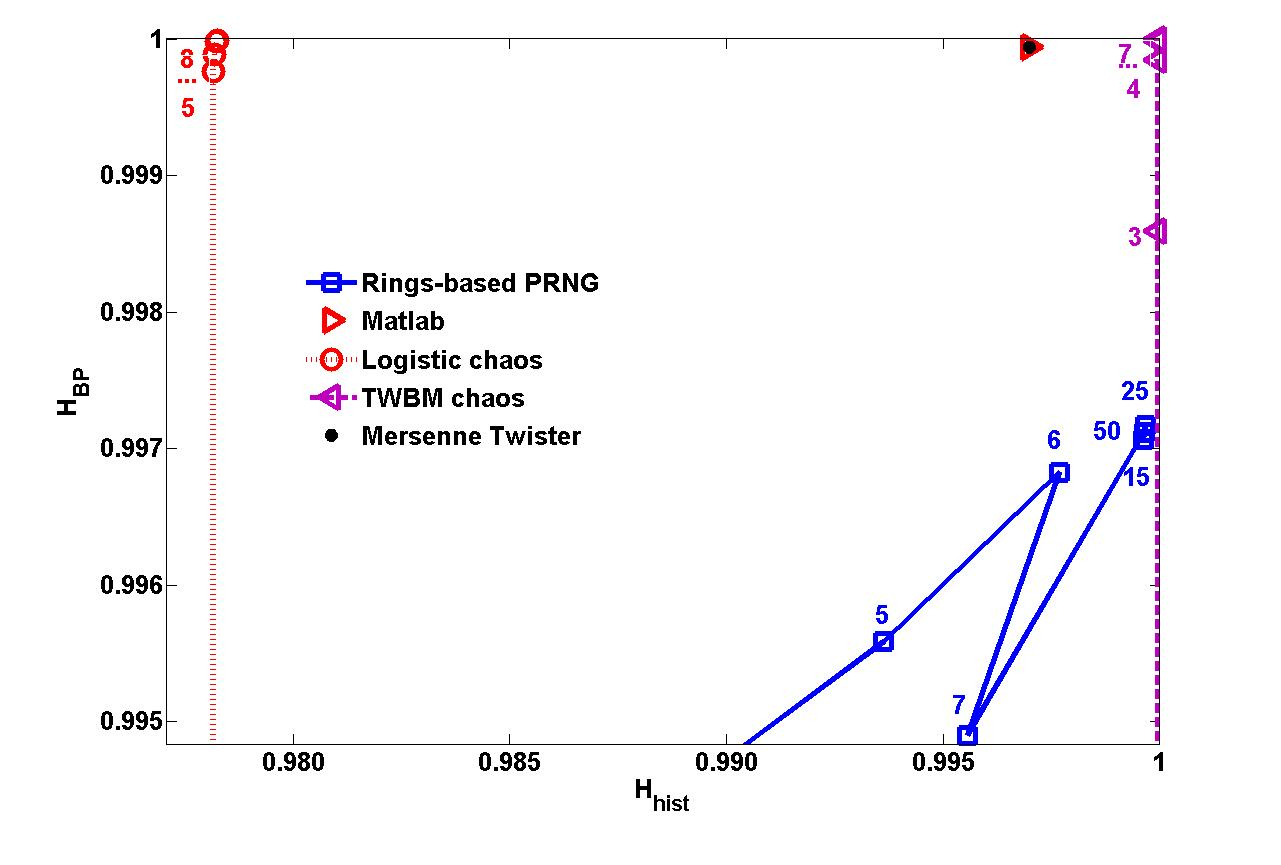
\includegraphics[ width=0.8\textwidth]{HhistvsHBP_z}
\caption{Zoom of Fig. \ref{fig:HBPvsHhis_all}  around the ideal point $(1,1)$ of the $H_{BP}$ vs $H_{hist}$ plane. Numbers next to each square indicate the number of \emph{RO}s used in that rings-based \emph{PRNG}. Numbers next to each point in the chaotic sequences indicate the number of iteration of the chaotic map.} \label{HhistvsHBP_zoom}
\end{center}
\end{figure*}
%=========================================

There, it is shown the evolution of the \emph{RO}-based \emph{PRNG} sequences when the quantity of \emph{RO}s increases from $5$ to $50$ (numbers next to each square). It can be seen that as the number of rings increases, data increase their mixture and also the histogram tends to be more uniform. So both properties are improved. Here a threshold in the number of rings can be determined, as the points saturate at about $(0.997,1)$, so this is the best \emph{PRNG} possible. Further, using more than $15$ \emph{RO}s presents no improvement.
As it was previously said, $H_{hist}$ quantifier detects the histogram variation of the sequence, and the $H_{BP}$ quantifier reflects the improvement in the mixing of data.
Finally, Mersenne Twister and Matlab sequences present identical value, ideal $H_{BP}$, and a high value of $H_{hist}$ nonetheless the histogram is not perfectly uniform (values are not equiprobable).

\subsection{Conclusions}
\label{sec:conclusions}
\emph{RO}-based \emph{PRNG} implemented here has demonstrated to satisfactorily meet the statistical properties desired by a \emph{PRNG}. They are comparable of other used \emph{PRNG}s and in some cases they are better. They employs few resources of the device and they are simply to implement in a digital platform.

It was demonstrated that for these architectures of \emph{PRNG} the quantity of
\emph{RO}s establishes \emph{PRNG}'s statistical properties. It was seen that
for $15$ \emph{RO}s both output's statistical properties, histogram
and mixing, were almost ideal, making unnecessary the increase of the number of rings.

The dual entropy plane proposed here has demonstrated to satisfactorily discern between the \emph{PRNG}'s two main desired properties, the equiprobability among all possible values and the statistical independence between consecutive values. Thus, it allows to clearly see what needs to be improved in a given sequence.



%\bibliographystyle{IEEEtran}
%\bibliography{xbibwebjulio2014_ingles,xbibMAXI_300314}  %


%%%%%%%%%%%%%%%%%%%%%%%%%%%%%%%%%%%%%%%%%%%%%%%%%%%%%%%%%%%%%%%%%%%%%%%%%%%%%%%%%%%%%%%%%%%%%%%%%

\section{Implementación de algoritmo genético para la búsqueda automática de caos en sistemas multiatractores (póster CASE2013)}

Se generó una lógica basada en algoritmos genéticos encargada de evolucionar los
parámetros del sistema de modo que cada generación tenga un comportamiento
caótico mejor que la anterior [3]. El target (fitness function), por lo tanto, es el MLE.
Para mayor claridad se separó el diagrama de flujo en dos partes, un diagrama principal
y una subrutina.
El sistema se inicializa en un conjunto de coeficientes llamado población inicial,
semilla o padre y se calcula su fitness function (Fp). Luego, se genera un incremento de
estos parámetros generando un hijo, que ingresa a la subrutina Evolution que lo
devuelve evolucionado y calcula su fitness function (Fc) para compararla con la de sus
padres. Las posibilidades son tres: el hijo es un padre de la siguiente generación
reemplazando al padre o no, o el hijo es descartado.
La subrutina Evolution es un algoritmo muy simple basado en mutaciones. Se
varían ligeramente los coeficientes del sistema (generando mutaciones) evaluando su
fitness function (Fm) buscando un máximo local.

\thispagestyle{empty}

\chapter{Cuantificadores de Aleatoriedad}

%%%%%%%%%%%%%%%%%%%%%%%%%%%%%%%%%%%%%%%%%%%%%%%%%%%%%%%%%%%%%%%%%%%%%%%%%%%%%%%%%
\section{Implementación de algoritmo genético para la búsqueda automática de caos (Póster CASE 2013)}

Se generó una lógica basada en algoritmos genéticos encargada de evolucionar los
parámetros del sistema de modo que cada generación tenga un comportamiento
caótico mejor que la anterior [3]. El target (fitness function), por lo tanto, es el MLE.
Para mayor claridad se separó el diagrama de flujo en dos partes, un diagrama principal
y una subrutina.
El sistema se inicializa en un conjunto de coeficientes llamado población inicial,
semilla o padre y se calcula su fitness function (Fp). Luego, se genera un incremento de
estos parámetros generando un hijo, que ingresa a la subrutina Evolution que lo
devuelve evolucionado y calcula su fitness function (Fc) para compararla con la de sus
padres. Las posibilidades son tres: el hijo es un padre de la siguiente generación
reemplazando al padre o no, o el hijo es descartado.
La subrutina Evolution es un algoritmo muy simple basado en mutaciones. Se
varían ligeramente los coeficientes del sistema (generando mutaciones) evaluando su
fitness function (Fm) buscando un máximo local.


%%%%%%%%%%%%%%%%%%%%%%%%%%%%%%%%%%%%%%%%%%%%%%%%%%%%%%%%%%%%%%%%%%%%%%%%%%%%%%%%%%%%%%%%%%%%%%%%%%%%

\section{Hardware Implementation of Maximum Lyapunov Exponent}


\subsection{Introduction}

The maximum Lyapunov Exponent characterizes how fast two
trajectories drift apart, if this rate is exponential the system
is said to be chaotic, because of this it is known as a detector
of ``chaoticity", \cite{strotgartz1994,Kantz1994,Sprott2003}.
Lately, the $MLE$ has been used in many applications, in very
different areas. Just to mention a few of them in \cite{Ma2013}
the Lyapunov exponent is used to judge the chaotic characteristic
of gas weak signal as the criteria for chaos, in
\cite{Bruijna2011} they studied  whether changes  in probability
of  falling  of  a simple  model  of human  walking (a so-called
dynamic  walker) could  be  predicted from $MLE$, in
\cite{Story2009} the author use  the Lyapunov exponents to predict
capsize events for both intact and damaged stability cases.

It becomes important to have a hardware implementation of a
quantifier that calculates the $MLE$. This work is part of a
larger and more complex project in which maximum Lyapunov exponent
of the data generated by a multiattractor non-linear system is
employed in order to increment the level of ``chaosticity" of the
system.

Multiattractor chaotic systems are a type of dynamics systems with
the peculiarity that their attractors critically depend on the
values of their parameters, \cite{strotgartz1994,Sprott2003}. This
becomes particularly risky when digital implementation is
performed, because the selection of the quantity of bits employed
to represent the system could entirely change the dynamics of it.
There are many quantifiers that detect this variations, depending
on which property is desired to be monitored. One of them is the
$MLE$.

This paper describes a design and hardware implementation of a
quantifier that calculates the maximum Lyapunov exponent of a
system, employing floating point arithmetic.


\subsection{Maximum Lyapunov exponent}

The Lyapunov exponents are quantifiers that characterize how the
separation between two trajectories evolves, \cite{Sprott2003}. It
is generally well known that chaotic behaviors are characterized
mainly by Lyapunov numbers of the dynamic systems. If one or more
Lyapunov numbers are greater than zero, then the system behaves
chaotically, otherwise, the system is stable. In this paper, we
employ the maximum Lyapunov number instead of each
Lyapunov number as it is one of the most useful indicators of
chaos.

The distance between trajectories changes in $2^{MLE}$ for each
iteration, on average. If $MLE<0$ the trajectories approaches,
this may be due to a fixed point, if $MLE=0$ the trajectories keep
their distance, this may be due to a limit cycle, if $MLE>0$, the
distance between trajectories is growing, and is an indicator of
chaos. \cite{Sprott2003}

There is a non-analytical way to measure it if only the inputs and
outputs of the system are accessible. The procedure is the
following: the system must be started from two neighbor points in
the phase plane, lets call them $(x_a,y_a)$ and $(x_b,y_b)$, as
the system is iterated the Euclidean distance between the two
trajectories is measured ($d_n$ in the $n_{th}$ sample) (eq.
\ref{eq:D0D1}), and the $b$ trajectory is relocalized on each
iteration  (eq. \ref{eq:reubicacion}), obtaining the points
$(x_{br},y_{br})$ to feed the system. Then the Lyapunov exponent
can be calculated as shown in eq. (\ref{eq:Lyapunov}). The process
can be seen in Fig. \ref{fig:relocalizacion}.


\begin{eqnarray}\label{eq:D0D1}
    d_{0(i-1)}&=& \sqrt{(x_{a(i-1)}-x_{br(i-1)})^2+(y_{a(i-1)}-y_{br(i-1)})^2}\nonumber\\
    d_{1(i)}&=& \sqrt{(x_{a(i)}-x_{b(i)})^2+(y_{a(i)}-y_{b(i)})^2}\\
\nonumber
\end{eqnarray}

\begin{eqnarray}\label{eq:Lyapunov}
    MLE &=& \frac{1}{n} \sum_{i=2}^{n} \log_2{\frac{d_{1(i)}}{d_{0(i-1)}}}
\end{eqnarray}


\begin{eqnarray}\label{eq:reubicacion}
    x_{br(i)}&=& x_{a(i)}+(x_{b(i)}-x_{a(i)})d_{o(i-1)}/d_{1(i)} \nonumber\\
    y_{br(i)}&=& y_{a(i)}+(y_{b(i)}-y_{a(i)})d_{o(i-1)}/d_{1(i)}
\end{eqnarray}




\subsection{Chaotic System analyzed}

In this case the system under analysis is a family of
bi-dimensional quadratic maps whose structure consists of a pair
of coupled quadratic difference equations (eq. \ref{eq:Quad-map}).
Each set of parameters $a_n$ and $b_n$, produces a different
evolution of the system. This characteristic is called
\textit{multiattractor}, and means that the chaotic behavior of
the system changes with the parameters selection, in Fig.
\ref{fig:atractores} can be seen three different attractors
corresponding to three different sets of parameters.
%%%%%%%%%%%%%%%%%%%%%%%%%%%%%%%%%%\cite{Antonelli uEA2012}.(Maxi)
{ \small
\begin{eqnarray}\label{eq:Quad-map}
    x_{(i+1)}&=& a_0 + a_1 x_{(i)} + a_2 x_{(i)}^2 + a_3 x_{(i)} y_{(i)} + a_4 y_{(i)}^2 + a_5 y_{(i)} \nonumber\\
    y_{(i+1)}&=& b_0 + b_1 x_{(i)} + b_2 x_{(i)}^2 + b_3 x_{(i)} y_{(i)} + b_4 y_{(i)}^2 + b_5 y_{(i)}\nonumber\\
\\
\nonumber \end{eqnarray}

}
%%%%%%%%%%%%%%%%%%%%%%%%%%Ver por que queda mal centrado el número(Maxi)

\begin{figure}
    \centering
    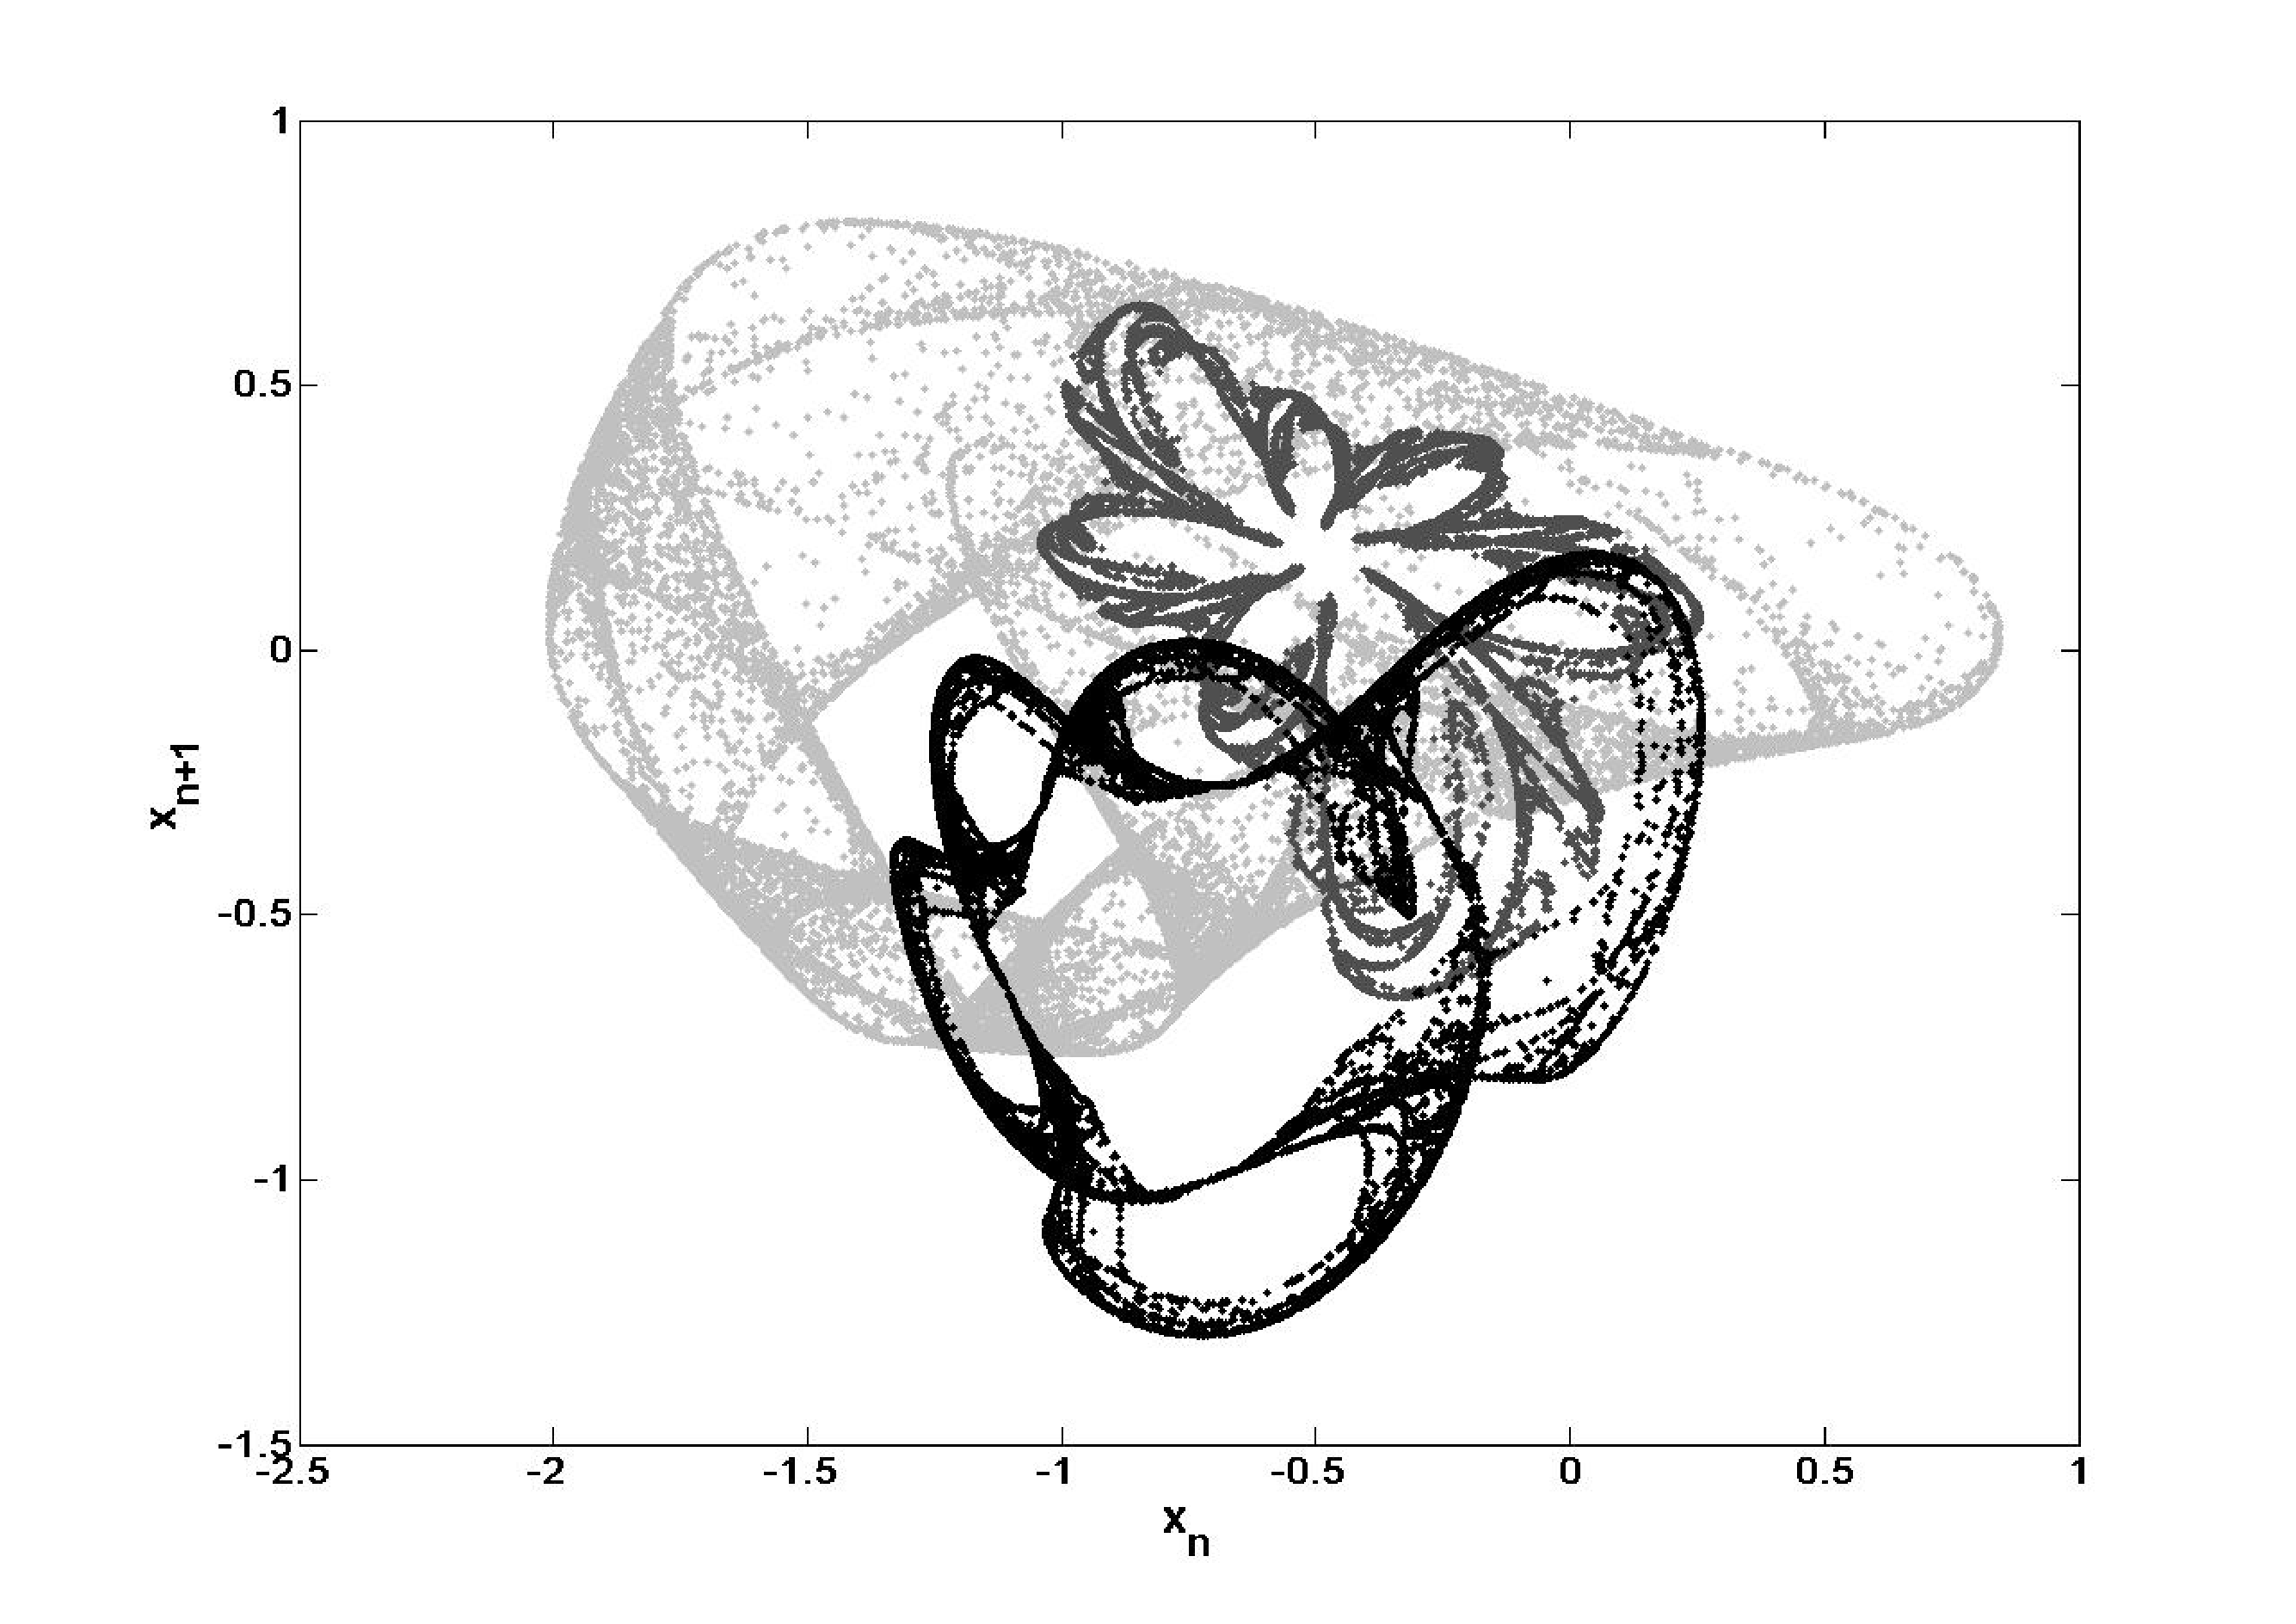
\includegraphics[width=1\columnwidth]{atractores.pdf}\\
    \caption{Three attractors for three different values for coefficients $a_n$ and $b_n$.}\label{fig:atractores}
\end{figure}
%%%%%%%%


In \cite{Antonelli2012}, the chaotic generator is explained in
detail. In order to be embedded in this design, the arithmetic
employed there had to be changed, switched to the IEE754 32-bits
floating point standard used here.



%%%%%%%%%%%%%%%%%%%%%%%%%%Ver por que queda mal centrado el número(Maxi)

\begin{figure}
    \centering
    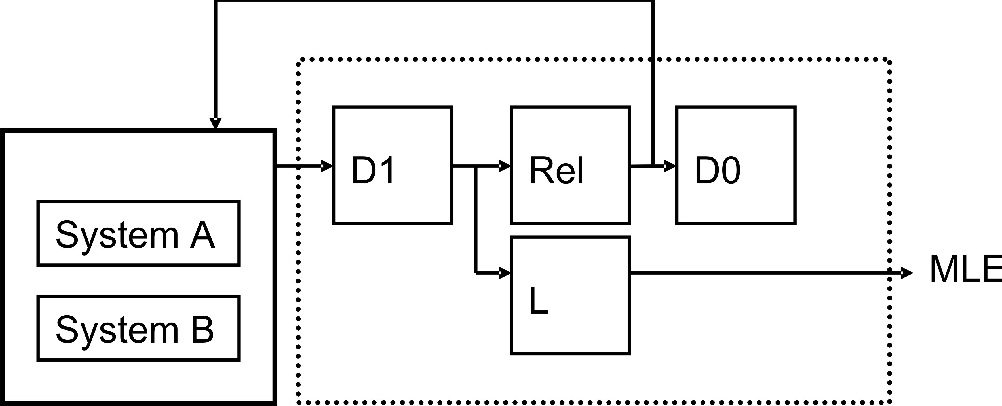
\includegraphics[width=1\columnwidth]{bloques.pdf}\\
    \caption{Enabling flow of the System.}\label{bloques}
\end{figure}
%%%%%%%%

\subsection{Design of the System}

In Fig. \ref{bloques} a block diagram of the enabling flow can be
seen. The system consists of four main blocks and is connected to
the chaotic system under test by a wishbone interface. This makes
the system independent of the quantifier and allows to easily
change the system being tested.

The system is duplicated in two blocks, $System A$ and $System B$,
each of them is initialized with points
($x_{a(i-1)}$,$y_{a(i-1)}$) and ($x_{br(i-1)}$,$y_{br(i-1)}$)
respectively, as explained before. When the chaotic systems finish
calculating the outputs, signal \textit{habilita} goes to zero and
 block $D_1$ is enabled to calculate the Euclidean distance of
those outputs, ($x_{a(i)}$,$y_{a(i)}$) and
($x_{br(i)}$,$y_{br(i)}$). Then, concurrent blocks $L$ and $Rel$
are enabled. The relocated points to feed $System B$ are
calculated by $Rel$ block. $Rel$ block only needs the current
value of $d_1$ and the previous value of $d_0$, as shown in eq.
\ref{eq:reubicacion}. When $x_{br(i)}$ and $y_{br(i)}$ are
available, $System$'s blocks are enabled to continue calculating
and get the next iteration, also block $D_0$ is enabled to
calculate the current value of $d_{0(i)}$ that will be employed in
the next iteration.

Finally, $L$ block is in charged of performing the division of
$d_0$ and $d_1$, then calculating the absolute value and
logarithmic of it. Before that it makes the addition of the
$N=250000$ outputs and divide them by $N$.

Each block was implemented using VHD language and also IP cores
provided by ALTERA (megafunctions, \cite{MEGAFUNCTIONS}) whenever
was possible, because this cores are optimized for this device.
Floating point operations such as sums, multiplications, absolute
values, logarithms were all calculated with the megafunctions
provided by ALTERA.


\begin{figure}
    \centering
    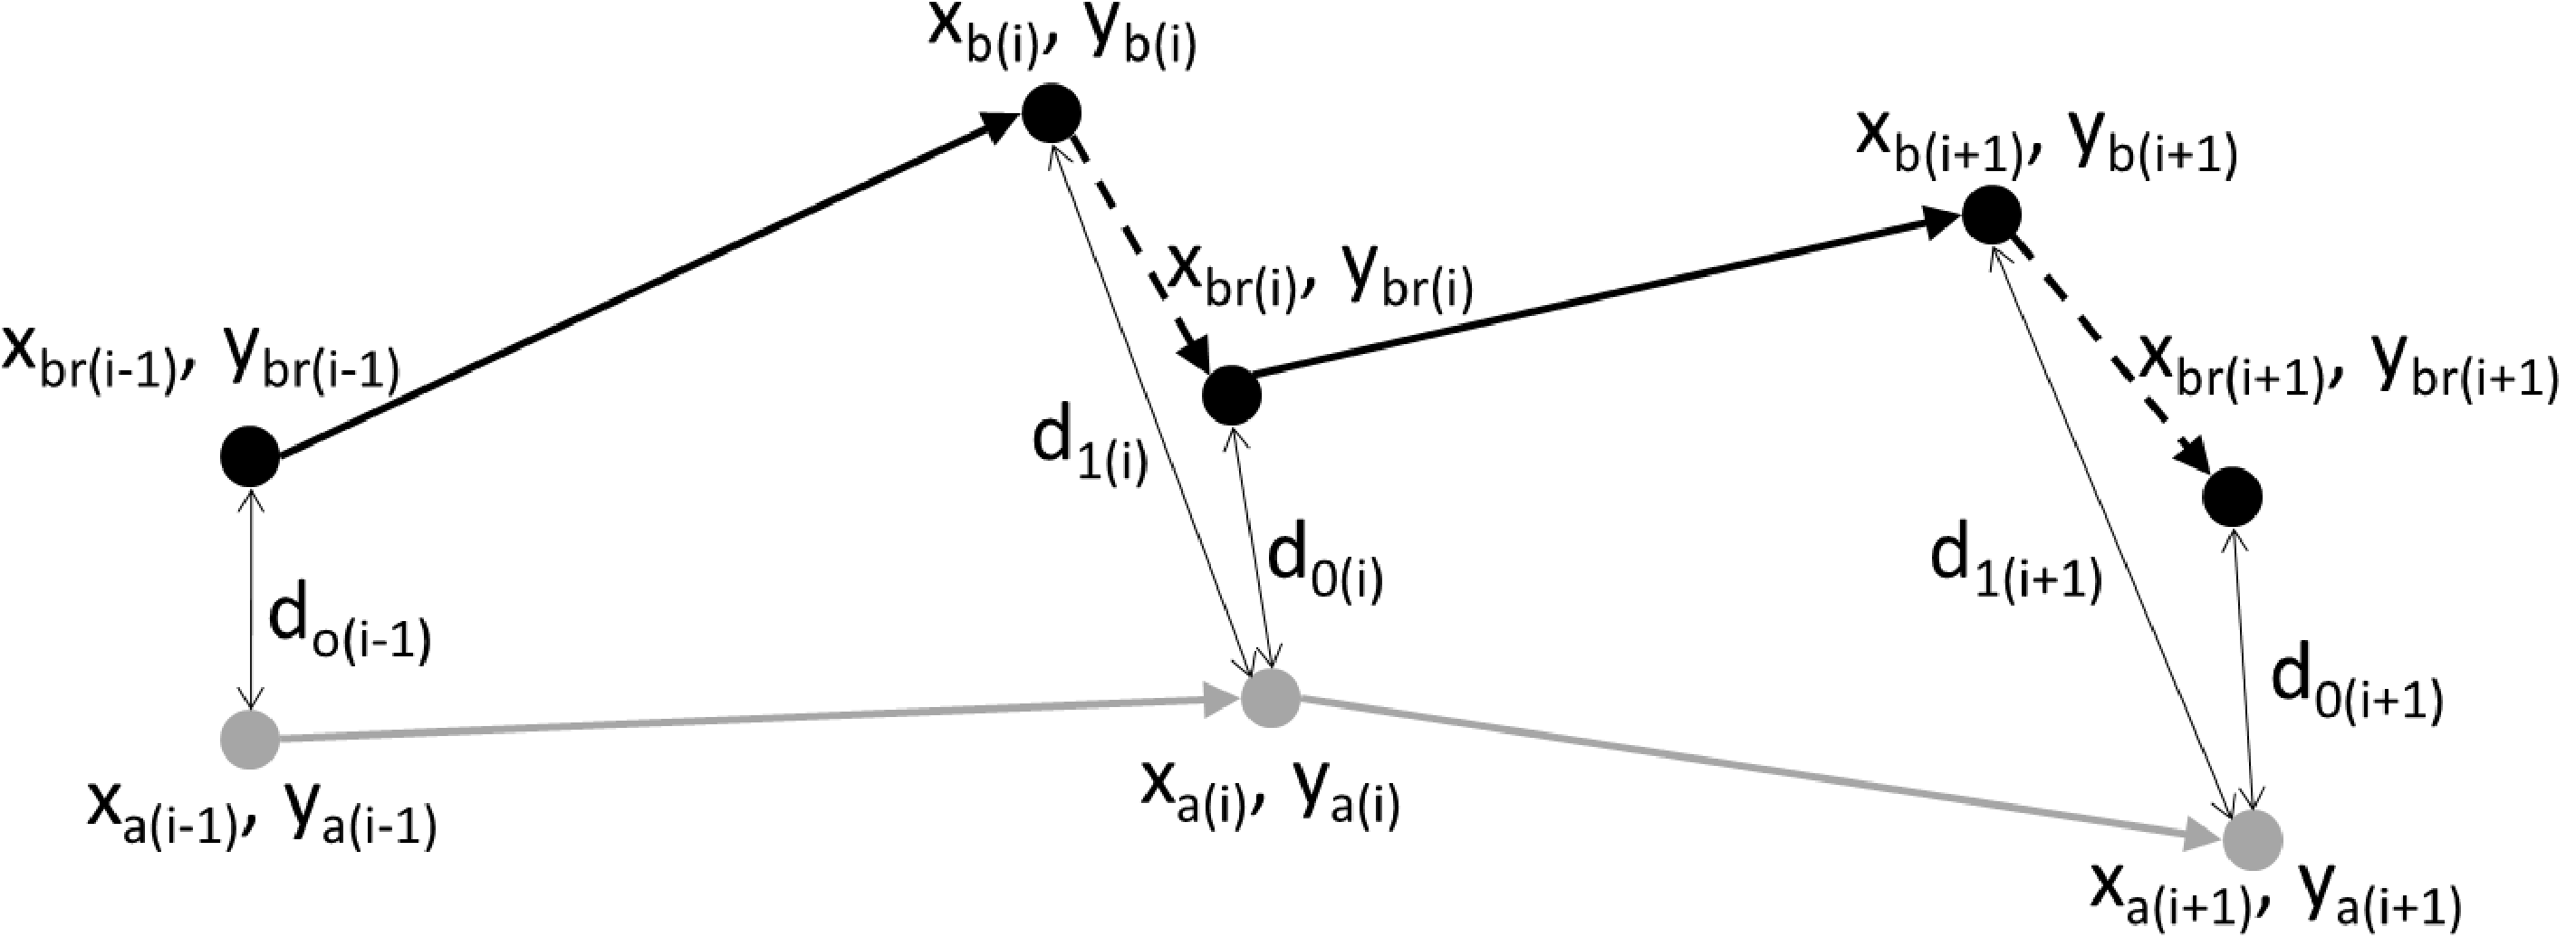
\includegraphics[width=1\columnwidth]{relocalizacion.pdf}\\
    \caption{Algorithm for calculating the Maximum Lyapunov exponent.}\label{fig:relocalizacion}
\end{figure}

 The working frequency of each
block is $clk$ and is provided by the $PLL$ in order to not to
overcome the maximum frequency allowed given by the Altera Timing
Analyzer, \cite{TimingALTERA}.

 In Fig. \ref{system} the hole system can be seen in Block Diagram/Schematic file of Quartus
 environment. There, block  $CTReset$ is a VHDL file that filters the rebound of
the power-on switch. It enables a PLL that decreases the operation
frequency, in order to meet the TimeQuest Timing Analyzer
 requirements. When this PLL locks the frequency it turns down $reset$ signal and the systems starts. As predicted by Fig.
\ref{bloques} blocks $Rel$ (called $Relocalizador$ in Fig.
\ref{system}) and $L$ are concurrent. The four blocks are designed
in the same way, an example is shown in Fig. \ref{D1} where it is
shown the implementation of $D1$ block. The inputs, points $a$ and
$b$, are taken each time signal \textit{habilita} goes down. Then,
the signals are processed according to eq. \ref{eq:D0D1} employing
Floating Point Altera Megafunctions \cite{ALTERAMEGAFUNCTIONS} to
calculate the Euclidean distance $d_1$. Internally, blocks $Rel$,
$L$ and $D0$ are the same as block $D1$, the only differences are
the operations they perform accordin to eqs. \ref{eq:reubicacion},
\ref{eq:Lyapunov} and \ref{eq:D0D1} respectively. These operations
are performed at the maximum frequency $clk$. Outputs of block $L$
are for testing purposes, the final design will just keep $L\_sal$
output.

\begin{figure*}
    \centering
    \includegraphics[width=1.7\columnwidth]{circuito.jpg}\\
    \caption{Hole System in Block Diagram/Schematic file of Quartus environment.}\label{system}
\end{figure*}


\begin{figure*}
    \centering
    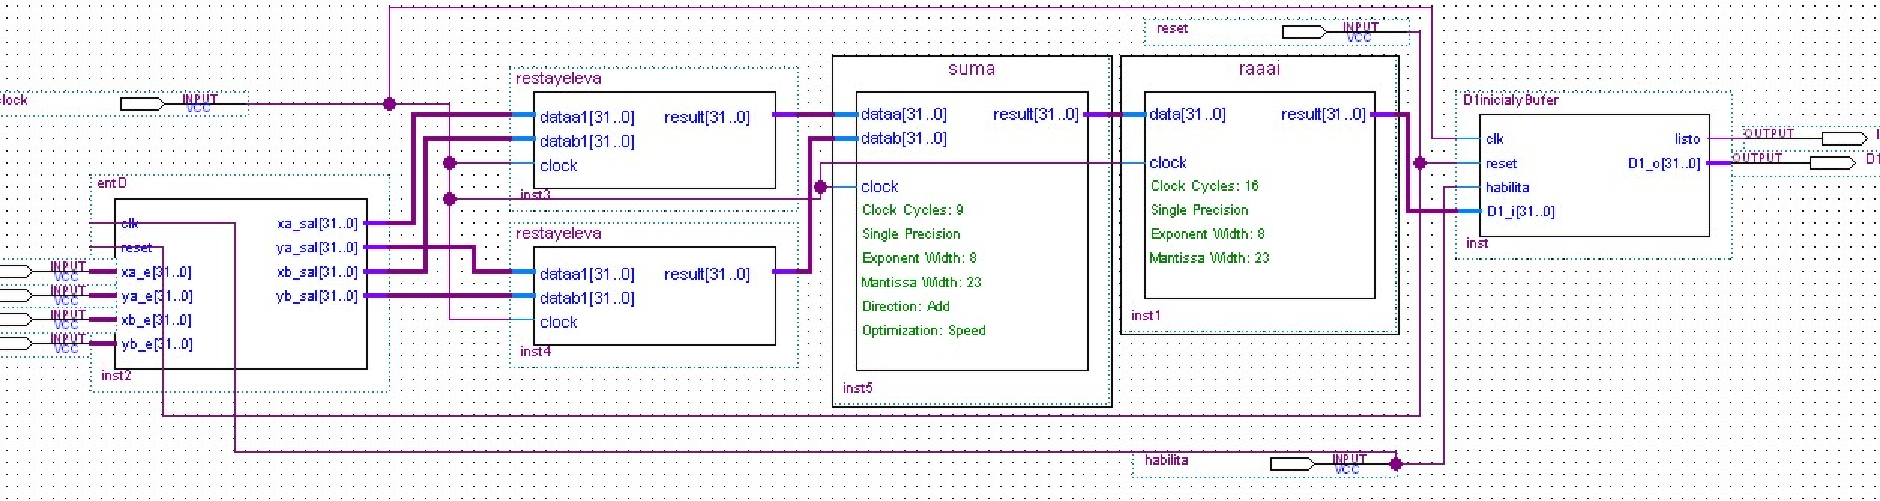
\includegraphics[width=2\columnwidth]{D1.pdf}\\
    \caption{$D_1$ block in Block Diagram/Schematic file of Quartus environment.}\label{D1}
\end{figure*}

\begin{figure*}
    \centering
    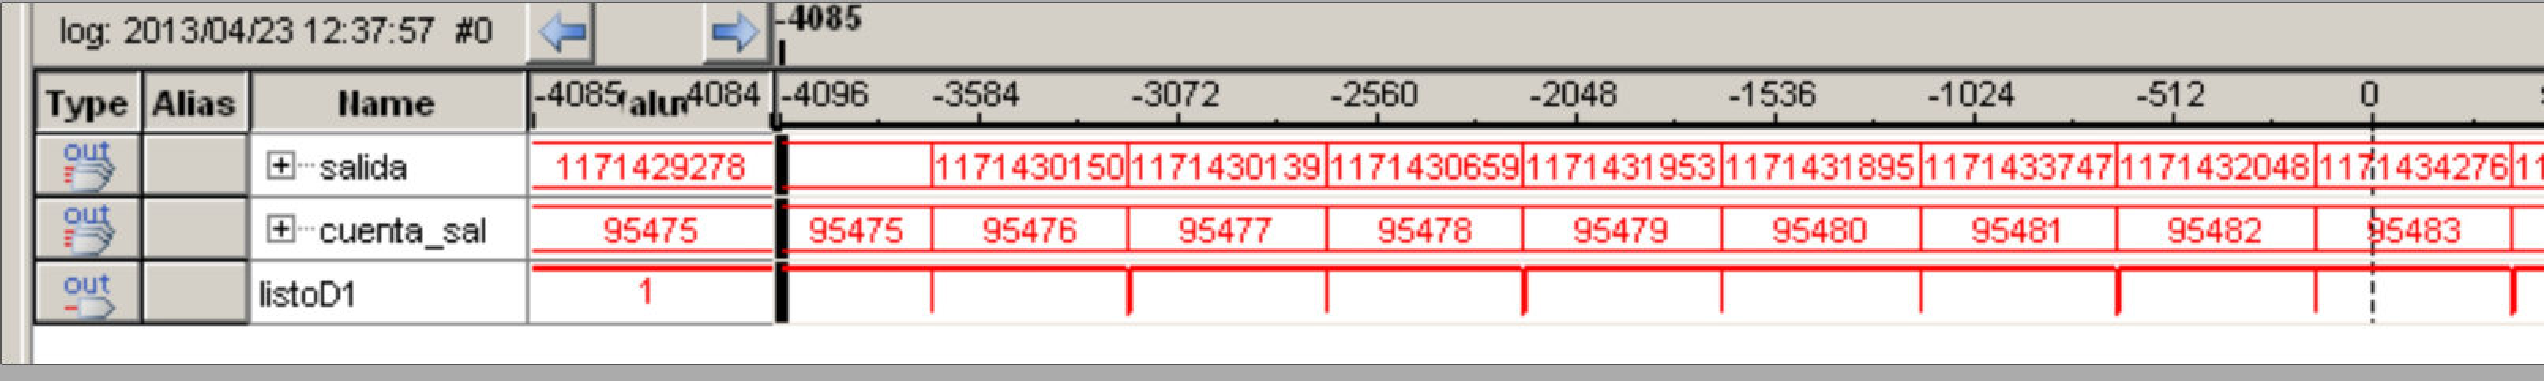
\includegraphics[width=2.1\columnwidth]{st.pdf}\\
    \caption{Quartus Signal Tap output.}\label{st}
\end{figure*}

\subsection{Results}

The system is  synthesized and experimentally  verified on the
Altera CYCLONE III FPGA and the results are shown in Fig.
\ref{compilacion}. The Timing Analysis reports that the frequency
must be at the most $84.95$MHz, so the clock of the board
($125$MHz) had to be divided to solve this limitation. A PLL
provided by Altera, \textit{ALTPLL} \cite{MEGAFUNCTIONS}, was
employed to divide the frequency of the board
 by $2$ ($reloj$ block of Fig. \ref{system}).

The Compilation Report (Fig. \ref{compilacion}) shows that the
logic utilization does not exceed 25\% this means $29307$ total
logic elements. 54\% of the total memory bits and 8\% of the
$9$-bit embedded multiplier.
%Interestingly, % the  16-bit

\label{sec:resultados}
\begin{figure}
    \centering
    \includegraphics[width=1\columnwidth]{lyap_MATLAB.jpg}\\
    \caption{Output of the system $MLE$.}\label{lyapu}
\end{figure}

In Figure \ref{st} the Signal Tap output can be seen. There, three
signals are shown: the one called \textit{salida} is the sum of
$MLE$ on each iteration (eq. \ref{eq:Lyapunov}). The second signal, called
\textit{cuenta\_sal} corresponds to the number of the current sum.
Finally, each falling edge of the signal \textit{listoD1}
indicates that the output is valid. The output is expressed in
IEE754 32-bits floating point standard, so the data was processed
with Matlab to obtain the Lyapunov curve seen in Fig. \ref{lyapu}. The value of $MLE$ at sample $250000$ is $ 0.1415$ and it is consistent with the $MLE$ obtained using Matlab.



\begin{figure}
    \centering
    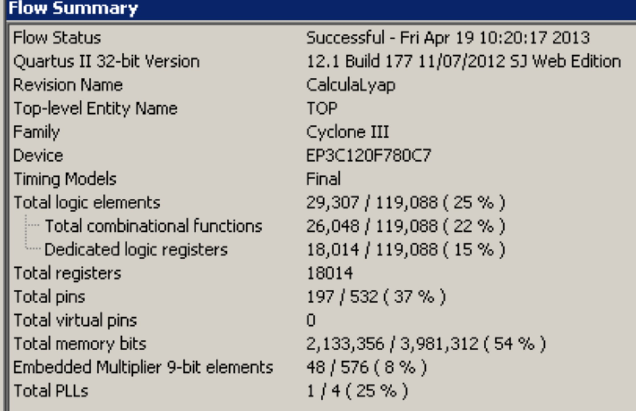
\includegraphics[width=1\columnwidth]{compilacion.pdf}\\
    \caption{Quartus Compilation report.}\label{compilacion}
\end{figure}


\subsection{Conclusions}
\label{sec:conclusions}

From the results presented herein, it is possible to conclude that
the developed quantifier accurately calculates the $MLE$ of a
system. We exploit the underline parallel nature of the $MLE$
computation equations with the aim of optimizing the proposed
architecture design, allowing its concurrent implementation based
on FPGA technology.

%\bibliographystyle{IEEEtran}
%\bibliography{xbibWEBjun2012_ingles}

%%%%%%%%%%%%%%%%%%%%%%%%%%%%%%%%%%%%%%%%%%%%%%%%%%%%%%%%%%%%%%%%%%%%%%%%%%%%%%%%%%%%%%%%%%

\section{Causal and Non-causal Entropy quantifiers implemented in FPGA}

\subsection{Introduction}
\label{sec:Intro}
In the development of new electronic realizations of NonLinear Systems, specially Multiatractor chaotic Systems it is critical to be able to know and monitor the system's properties. Always a thorough analysis of the systems is required to meet the objectives, mainly the changes in the statistical properties induced by discretization of the system. Then it is necessary to check that the system still satisfies the application's requirements, this demands further analysis. Tools coming from the nonlinear analysis like Lyapunov exponents, cross, and autocorrelation, Perron-Frobenius operator, Correlation Dimension are employed, and also statistical tools like the Shannon Entropy, Complexity, Bandt and Pompe
embedding.

This work is part of a more ambitious project, which is the hardware development and implementation of tools for the analysis of nonlinear systems. These tools will mean a significant advance in the field of implementation of nonlinear systems. It will allow to more accurately understand and describe the behavior of the digital version of this type of systems. The complete package of tools that we intend to implement consists of:
\begin{itemize}
\item functional of the probability distribution: Shannon Entropy, Statistical Disequilibrium, and Statistical Complexity;
\item time series's quantifiers, especially Lyapunov exponents, autocorrelation, cross-correlation and fractal dimensions;
\item Perron-Frobenius operator, quantifiers of recurrent plots;
\item Statistical tests proposed in standardized banks for studying random number generators (Marsaglia, NIST, etc.).
\end{itemize}

At the moment, there is no much literature on hardware implementations of these tools \cite{DeMicco2013}.

In the particular case of entropy, it is used in various applications, such as in the anomaly detection of IP data flows \cite{Gu2005, Wagner2006}. In \cite{Subramanya2008} an FPGA design and simulation of an entropy quantifier is introduced, however currently there are no available hardware implementations of this quantifier.

Within the project mentioned in this paper a system that calculates the entropy of a particular probability distribution (PDF) associated with a data set is implemented. Causal and non-causal PDFs are analyzed. Data can have a digital source (generated by code) or can come from sampling external analog signals. The development board used the \textit{M1AFS-embedded kit}, based on the \textit{M1AFS1500} chip that is known for having an analog block embedded in the same package of the FPGA.

Then, the numerical accuracy of the implemented quantifier is verified  by comparing their results with a standard program. The maximum error detected determines the statistical accuracy of the system.

The organization of this paper is as follows: Section \ref{sec:entropias} both normalized entropies are presented for their consideration; Section \ref{sec:Hardware} describes the hardware implementation and interfaces; in \ref{sec:Software} the software is described in detail; Section \ref{sec:resultados} shows the obtained results of the system validation and in the measurement of the signals. In section \ref{sec:discusion}, experimental results are interpreted and discussed. Finally, we present our conclusions in Section \ref{sec:conclusiones}.

\subsection{Causal and Non causal Entropy}
\label{sec:entropias}
Let $X=\{x_i, i=1,...,N\}$ of length $N$ the output of a given source symbol, 
with alphabet $\mathcal{A}=\{a_i,i=1,...M\}$. Each element of $X$ is $x_i \in \mathcal{A}$.

The most commonly used \emph{PDF} is the normalized histogram of the $N$ values of $X$ between the $M$ symbols of $\mathcal{A}$; it is defined as $PDF_{hist}=\{p_i,i=1,...M\}$, where $p_i$ 
is the probability of occurrence of the symbol $a_i \in \mathcal{A}$. Its normalized Shannon entropy is referred to as   $H_{hist}$ and is defined:

\begin{equation}
\label{eq:entropia}
H_{hist}=\frac{\sum_{i=1}^{M}{p_i~log~p_i}}{logM}
\end{equation}

The standard entropy $H_{hist}$ quantifies the distribution of the elements of the series among all possible symbols.

If the source is a Pseudo Random Number Generator (PRNG), then all the symbols of the alphabet should appear the same number of times and its (optimal) value will be $H_{hist}=1$.

$PDF_{hist}$ is non-causal since it does not consider the temporal order of  time series' elements. This fact means that the $X$ vector could be rearranged to generate other vector $Y$, which would have the same histogram as $X$, and, therefore identical $PDF_{hist}$ and the same value for $H_{hist}$.

For quantifying statistical independence between consecutive elements, in this paper the causal PDF proposed by Bandt \& Pompe in \cite{Pompe2002} is used.
This PDF is obtained by assigning patterns of order to overlapped segments of length $D$ of the time series.

The process for its calculation is the following: first $D$ consecutive elements are grouped $\{x_i,x_{i+1},...,x_{i+D}\}$. Then the (ascending or descending) order of the $D$ values of each group is compared to the order of the vector $\{1,2,...,D\}$. There are $D!$ Possible ways to sort the numbers  $\{1,2,...,D\}$. If two values of $x_i$ within the same group are identical, it is considered that the first is lower, to obtain a unique result. Each permutation is called \emph{ordering pattern}\cite{Amigo2006}. 

The normalized histogram of the order patterns is the causal Bandt \& Pompe's PDF $PDF_{BP}$. The normalized Shannon entropy of that $PDF_{BP}$ is $H_{BP}$ where the subscript $BP$ means ``Bandt \& Pompe''.

Bandt and Pompe suggest $3\leq D \leq7$. For this work, we adopted $D=6$.

In the $H_{BP}$ vs. $H_{hist}$ plane \cite{DeMicco2008}, a higher value in any of the entropy values implies an increase in the uniformity of the involved $PDF$. The point $(1,1)$ represents an ideal case were both distributions, distribution of values and distribution of order patterns, are uniform.

A complete discussion about the convenience of using these quantifiers is beyond the scope of this work. A broad study can be found in \cite{DeMicco2008,Wackerbauer1994,Lopez1995,Rosso2007A,Rosso2009}.

\subsection{Implemented Hardware}
\label{sec:Hardware}

The hardware design was based on ACTEL's configuration on the 8051 microcontroller, and peripheral interfaces. It was developed using the software package \textit{Libero~Soc~v11.3\textsuperscript\copyright}. The development board used was \textit{M1AFS-EMBEDDED-KIT} that contains an FPGA \textit{M1AFS1500} and peripherals \cite{actelM1AFS1500}.

The \textit{M1AFS1500} embedded chip contains an analog block consisting of nine addressable adapters of four inputs each, a 32 inputs analog multiplexer and a configurable analog-digital converter.

For handling this block, a system also provided by ACTEL is used. This system is based on an 8051 microcontroller, and it  also contains drivers of the peripheral among other things \cite{Core8051sS,Core8051sH}.

The developed system can be divided into three main stages as shown in Fig. \ref{Fig:Sistema}: the first phase is the Acquisition, which converts the incoming analog signals into digital words. The next step is the Calculation logic stage, it uses the SRAM to perform calculations and coordinate the interfaces, and the last stage is the Presentation which sends the results to a computer through the USB-to-UART interface.

\begin{figure}
 \centering
 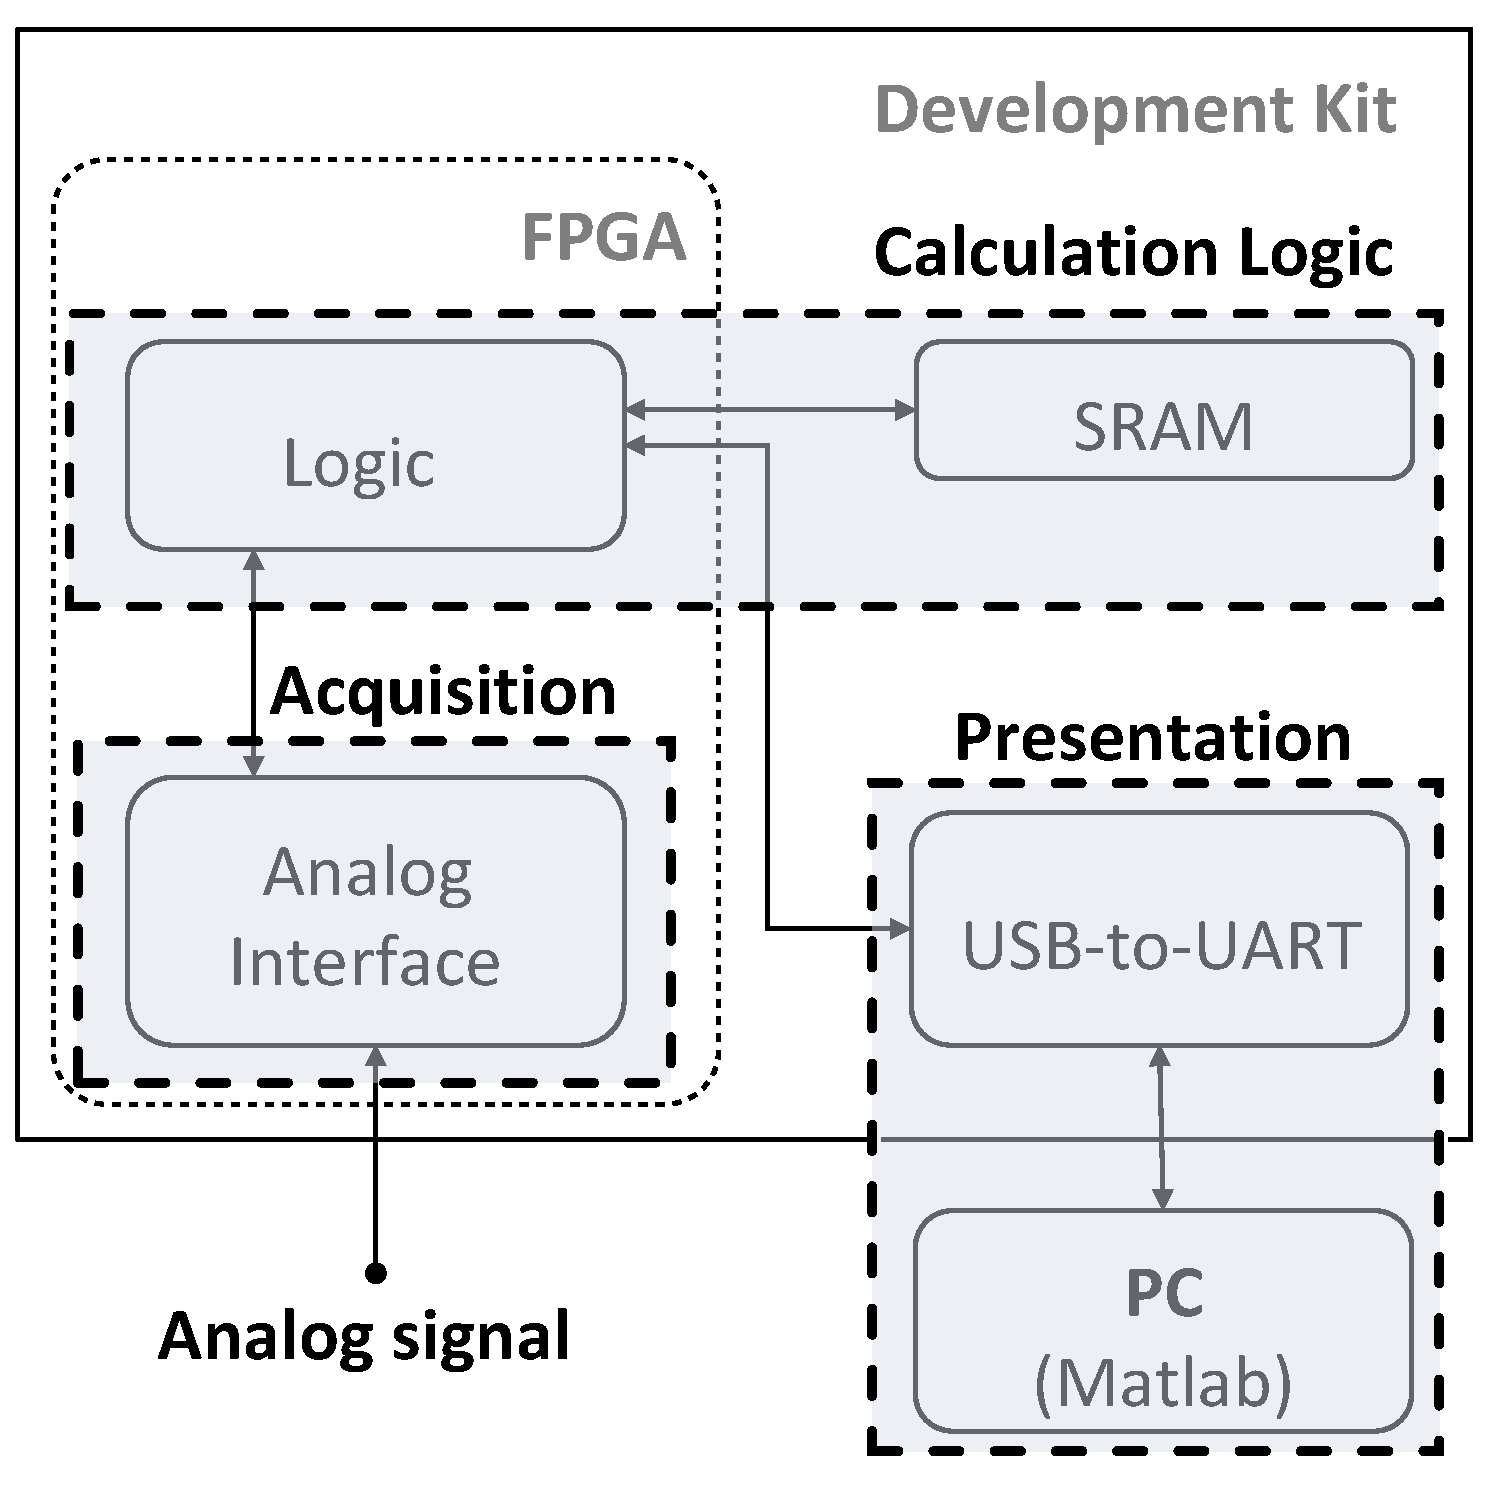
\includegraphics[width=.8\columnwidth]{Sistema_edit.pdf}\\
 \caption{Scheme of the complete system.}\label{Fig:Sistema}
\end{figure}
%
\subsubsection{Acquisition Stage}
%
The analog data to be evaluated is entered into the system by using the voltage input $AV2$ of the analog block \textit{Analog~Quad~2}. 
This input is mapped to channel seven of the analog multiplexer, and it was configured with an input voltage of 0~V to 4~V.
The analog-digital converter was configured with a 12-bit resolution. In this first prototype the maximum sample rate achieved was 16~ks/s, limited by the processing logic delay. This speed was enough for the required measurements. However, in a next stage an optimization of the design will be developed by increasing the operating frequency, among other improvements.

\subsubsection{Calculation logic}
%
The calculations and synchronization between peripherals are made at this stage. Figure \ref{fig:logica} shows the main blocks that compose it.

\begin{figure}
 \centering
 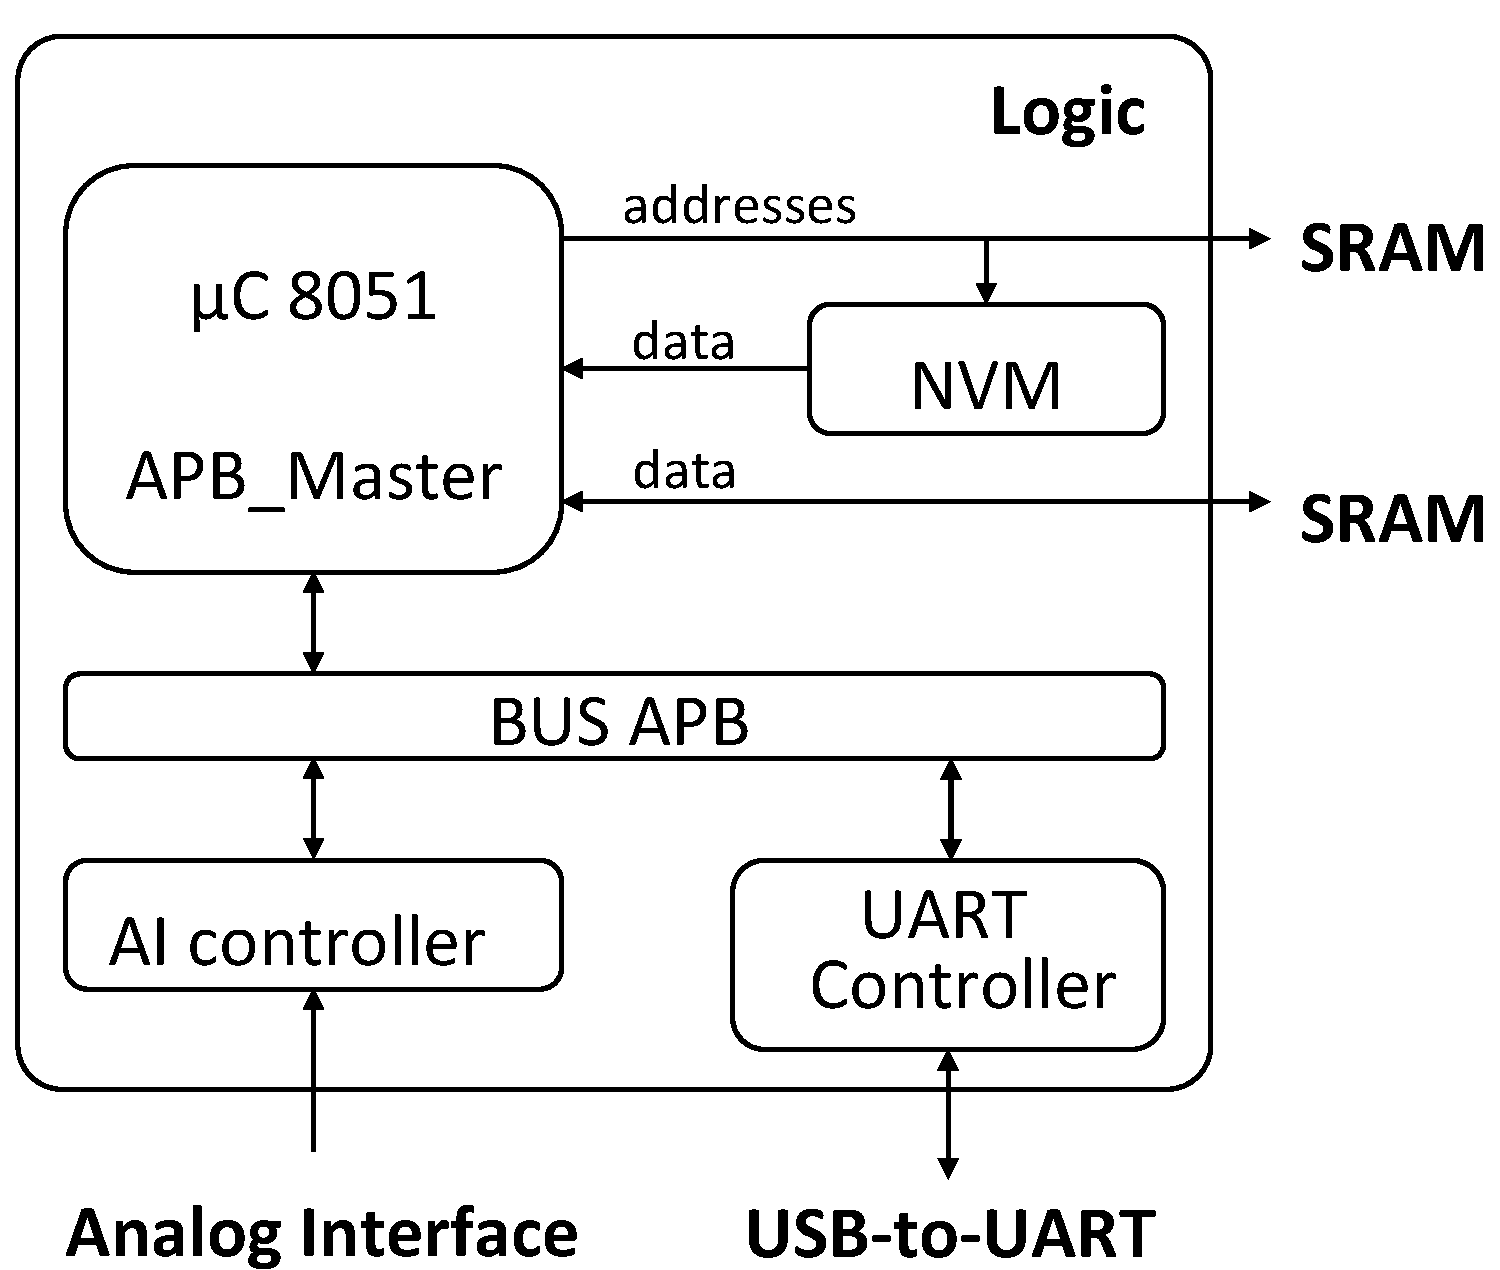
\includegraphics[width=.85\columnwidth]{Logica_edit.pdf}\\
 \caption{Details of the Calculation Logic stage.}\label{fig:logica}
\end{figure}

The heart of implementation is an 8051 Core that provides  Actel in its library catalog. It is a microcontroller containing the central logic of the Intel 8051 microprocessor, without its peripherals.
This micro has a Harvard architecture with a 16~bits address bus, limiting our design to 64~KB of memory code and 64~KB of data memory.

The application that performs the calculations presented in section \ref{sec:entropias} runs over this microcontroller.
It is responsible for obtaining the PDFs (BP and hist) and to perform the calculations to get the entropies from the input data, according to Eq. \ref{eq:entropia}. Section \ref{sec:Software} describes in detail the developed software.
In this particular FPGA, the code memory is a non-volatile memory (NVM) and is implemented in the internal flash of the FPGA blocks. It is mapped onto the addresses from 0x0000 to 0xFFFF and is written  during compilation with the contents of a hexadecimal format file.

The system functionality is extended by connecting peripherals through the APB interface.

For handling communication with the PC, the UART controller is used. The output of this block is directed out of the FPGA and is connected to a USB-to-UART chip that is soldered to the board.
The analog block is controlled by the AI controller, which routes and synchronizes its inputs.

%
\subsubsection{Presentation}
The stage of data presentation involves the USB-to-UART chip adapter that is on the development board and is driven both by the program running on the FPGA as well as by the software that runs on the PC. 

The USB-to-UART chip is responsible for adapting the input-output UART logic to an input-output USB standard by which is possible to interact with the PC. Moreover, the program running on the PC handles the user interface and is described in detail in the next section.

\subsection{Implemented Software}
\label{sec:Software}

The system operation is achieved by the interaction of two programs. One running on the PC and another on the microcontroller instantiated in the FPGA. It can be seen a flow chart of the two programs and the interaction between them in Fig. \ref{fig.softflow}.
%
\begin{figure}[htpb]
\centering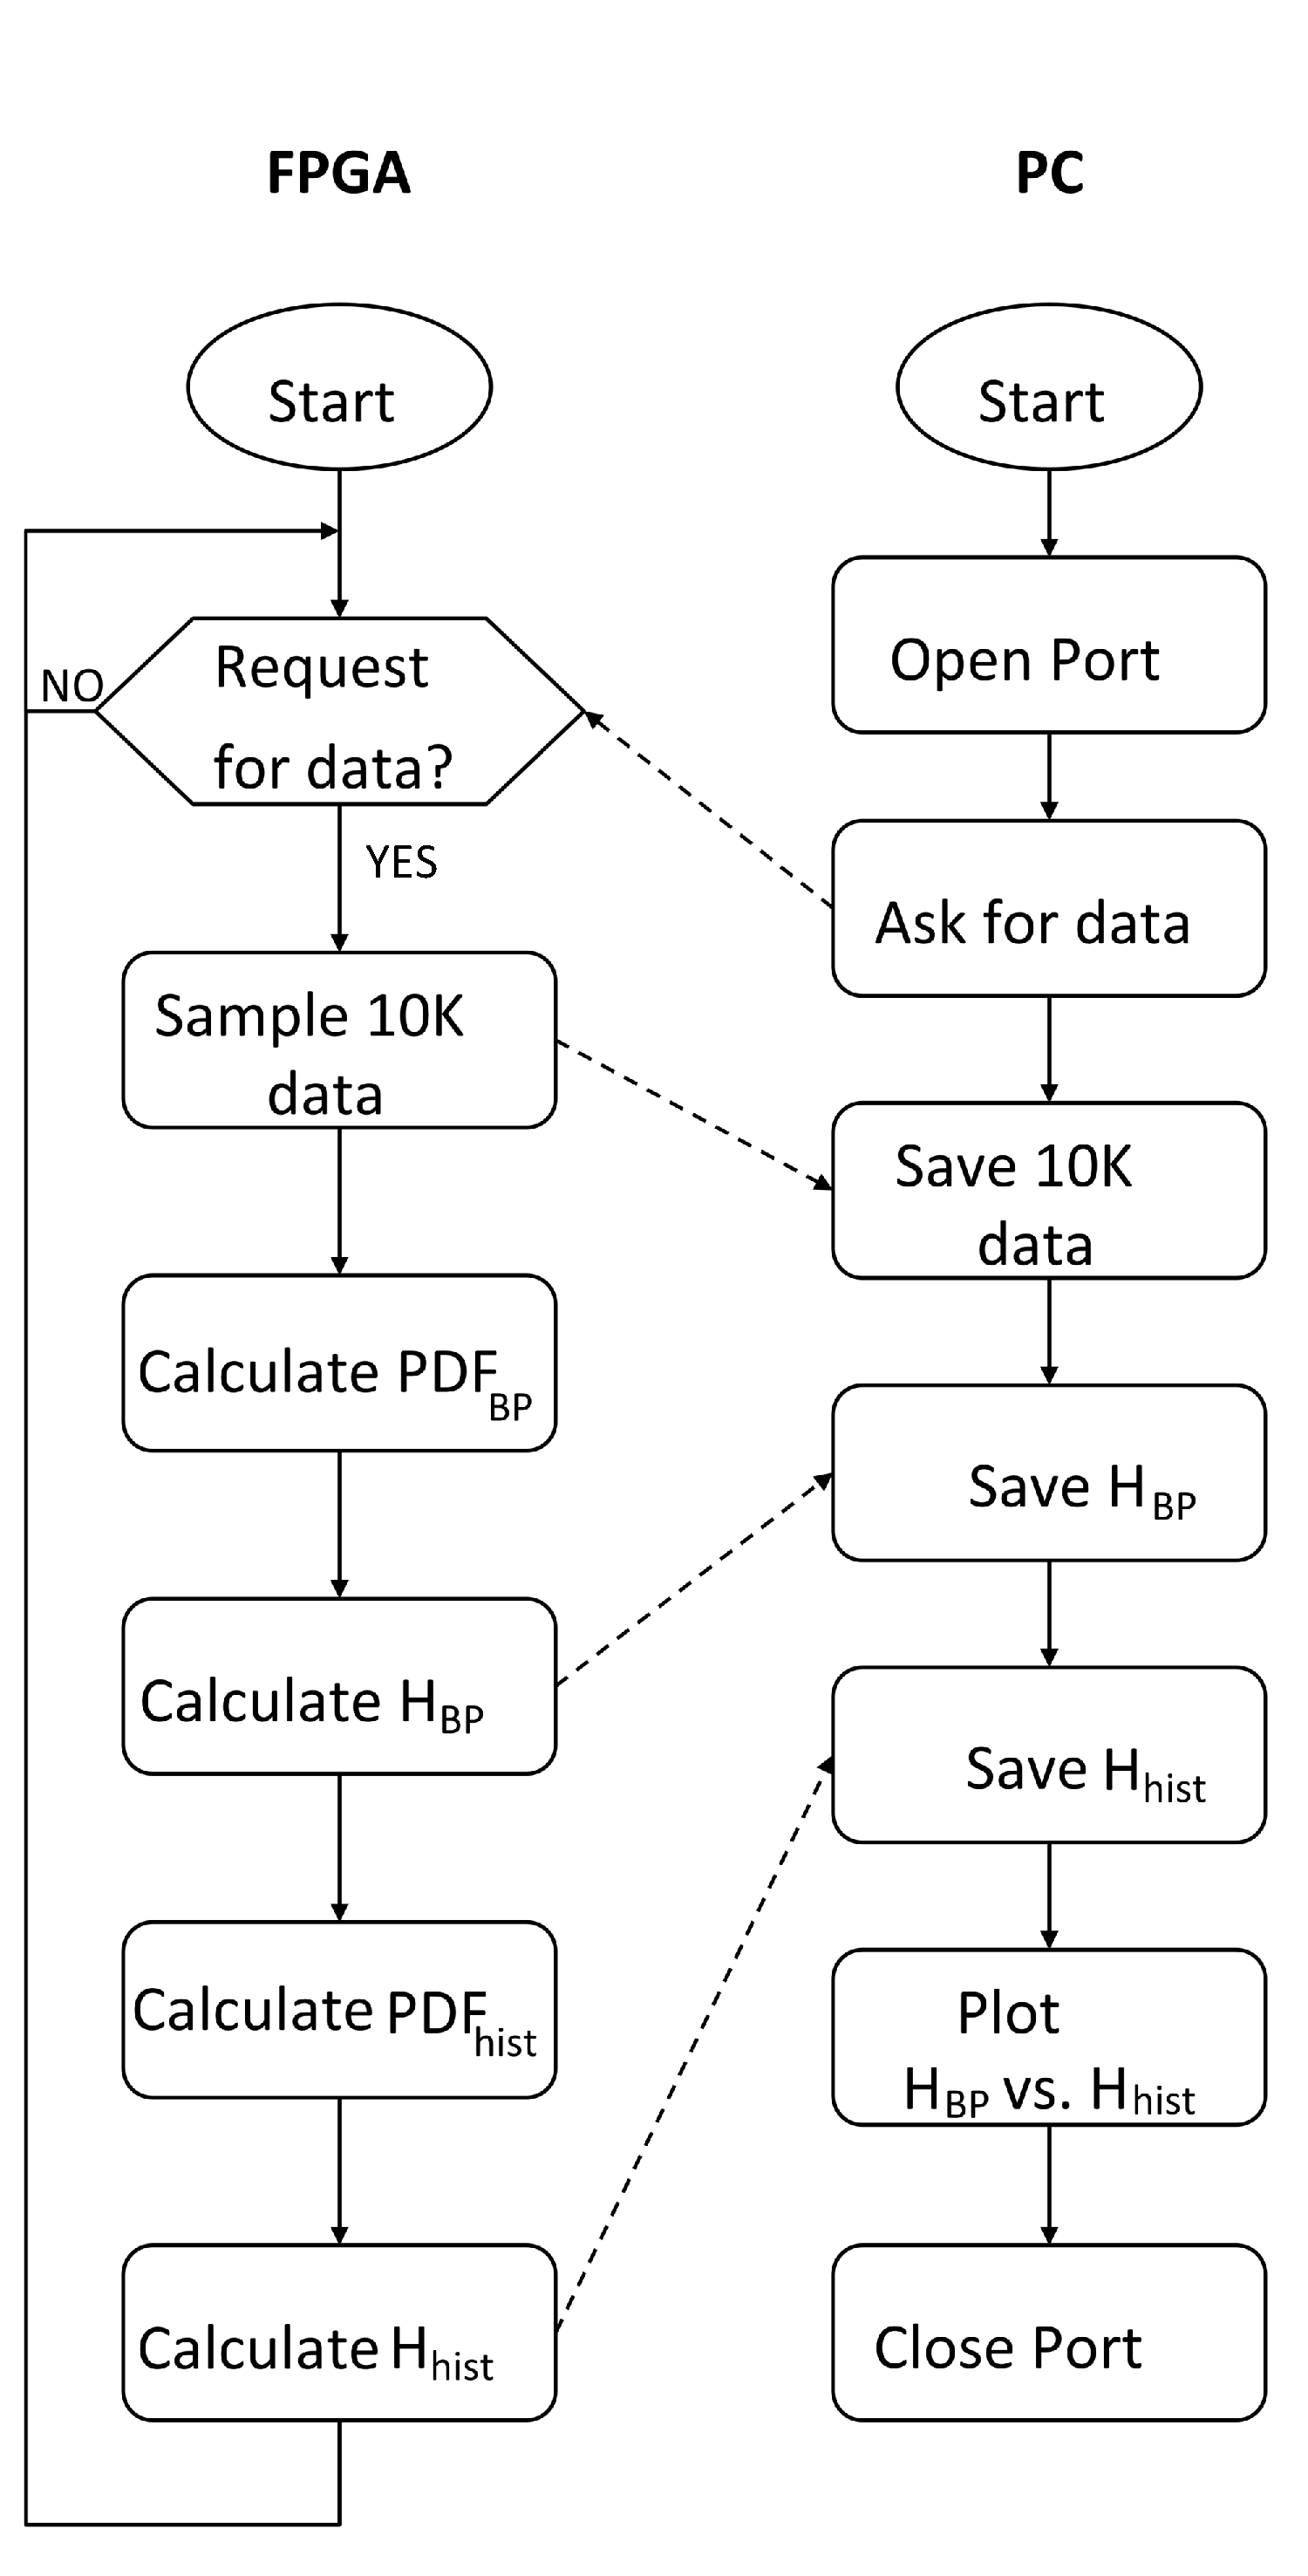
\includegraphics[scale=0.23]{Soft_edit2}
\caption{Flowchart of the implemented software.}\label{fig.softflow}
\end{figure}
On the PC runs a Matlab's script that is responsible for opening the serial port where the USB is mapped, requesting data, taking the results of the port, then plotting them in a plane $H_{BP}$ vs. $H_{hist}$ and finally closing the port.

Over the microcontroller instantiated in the FPGA runs a program written in C language and compiled for the 8051 microcontroller using the \textit{SoftConsole~IDE~v3.4\textsuperscript\copyright} tool. The firmware used is a modification of \cite{Core8051sS}. When a request for data from the UART port occurs, the data sampled in the analog input are stored. Then, $PDF_{hist}$ y $PDF_{BP}$ are calculated, and with this information, their respective entropies $H_{hist}$ and $H_{BP}$ are also calculated. These results are sent to the PC through the same port.

To validate the system, and verify how accurate the results are, the incoming sampled vector data is forwarded to the PC, so that it can calculate their entropies with PC using \textit{Matlab\textsuperscript\copyright} and compare them with the results of the implemented system.

\subsection{Results}
\label{sec:resultados}
As said, to test the system, the obtained results were compared with the results achieved by a pattern program running on the PC. For this, $10000$ samples of different waveforms were generated by both external (analog) and internal (digital) signals.

Two digital signals were produced by the code in the microcontroller, one corresponds to the rand() C function and the other to the chaotic Logistic map with parameter $r=4$.

Analog signals were generated with the \textit{HP33120A} waveform generator. With a range of $4~Vpp$ and $2~V$ of direct current to take advantage of the full spectrum of the analog-digital converter and increase the signal to noise ratio. In all four cases, the signal frequency was $100~Hz$ and the sampling rate of $16~ks/s$.

Table \ref{tabla} shows the absolute error between the calculated results of the quantifiers in the FPGA compared with the results calculated with the standard program running on the PC, over the same samples.

\begin{table}
\centering
\caption{Quantifiers error evaluated in the FPGA with respect to the results calculated by the pattern program.}\label{tabla}
\begin{tabular}{@{\extracolsep{\fill}}| c| c | c |c |}
 \hline
 \textbf{Generator} & \textbf{Source} & \textbf{Error $H_{BP}$} & \textbf{Error $H_{hist}$} \\
 \hline
Rand & Digital & $1,7421E^{-6}$ & $2,6977E^{-6}$ \\
 \hline
Logistic & Digital & $0,4256E^{-6}$ & $94,693E^{-6}$ \\
 \hline
Triangular & Analogic & $6,3445E^{-6}$ & $2,0028E^{-6}$ \\
 \hline
Sinusoidal & Analogic & $6,3151E^{-6}$ &$5,6506E^{-6}$ \\
 \hline
Square & Analogic & $0,1797E^{-6}$ & $1,9930E^{-6}$ \\
 \hline
Ramp & Analogic & $245,00E^{-6}$ & $1,0876E^{-6}$ \\
 \hline
\end{tabular}
\end{table}

Fig. \ref{fig:resultados} shows in the $H_{BP}$ vs. $H_{hist}$ plane the results calculated by the FPGA.

\begin{figure}[htb]
\centering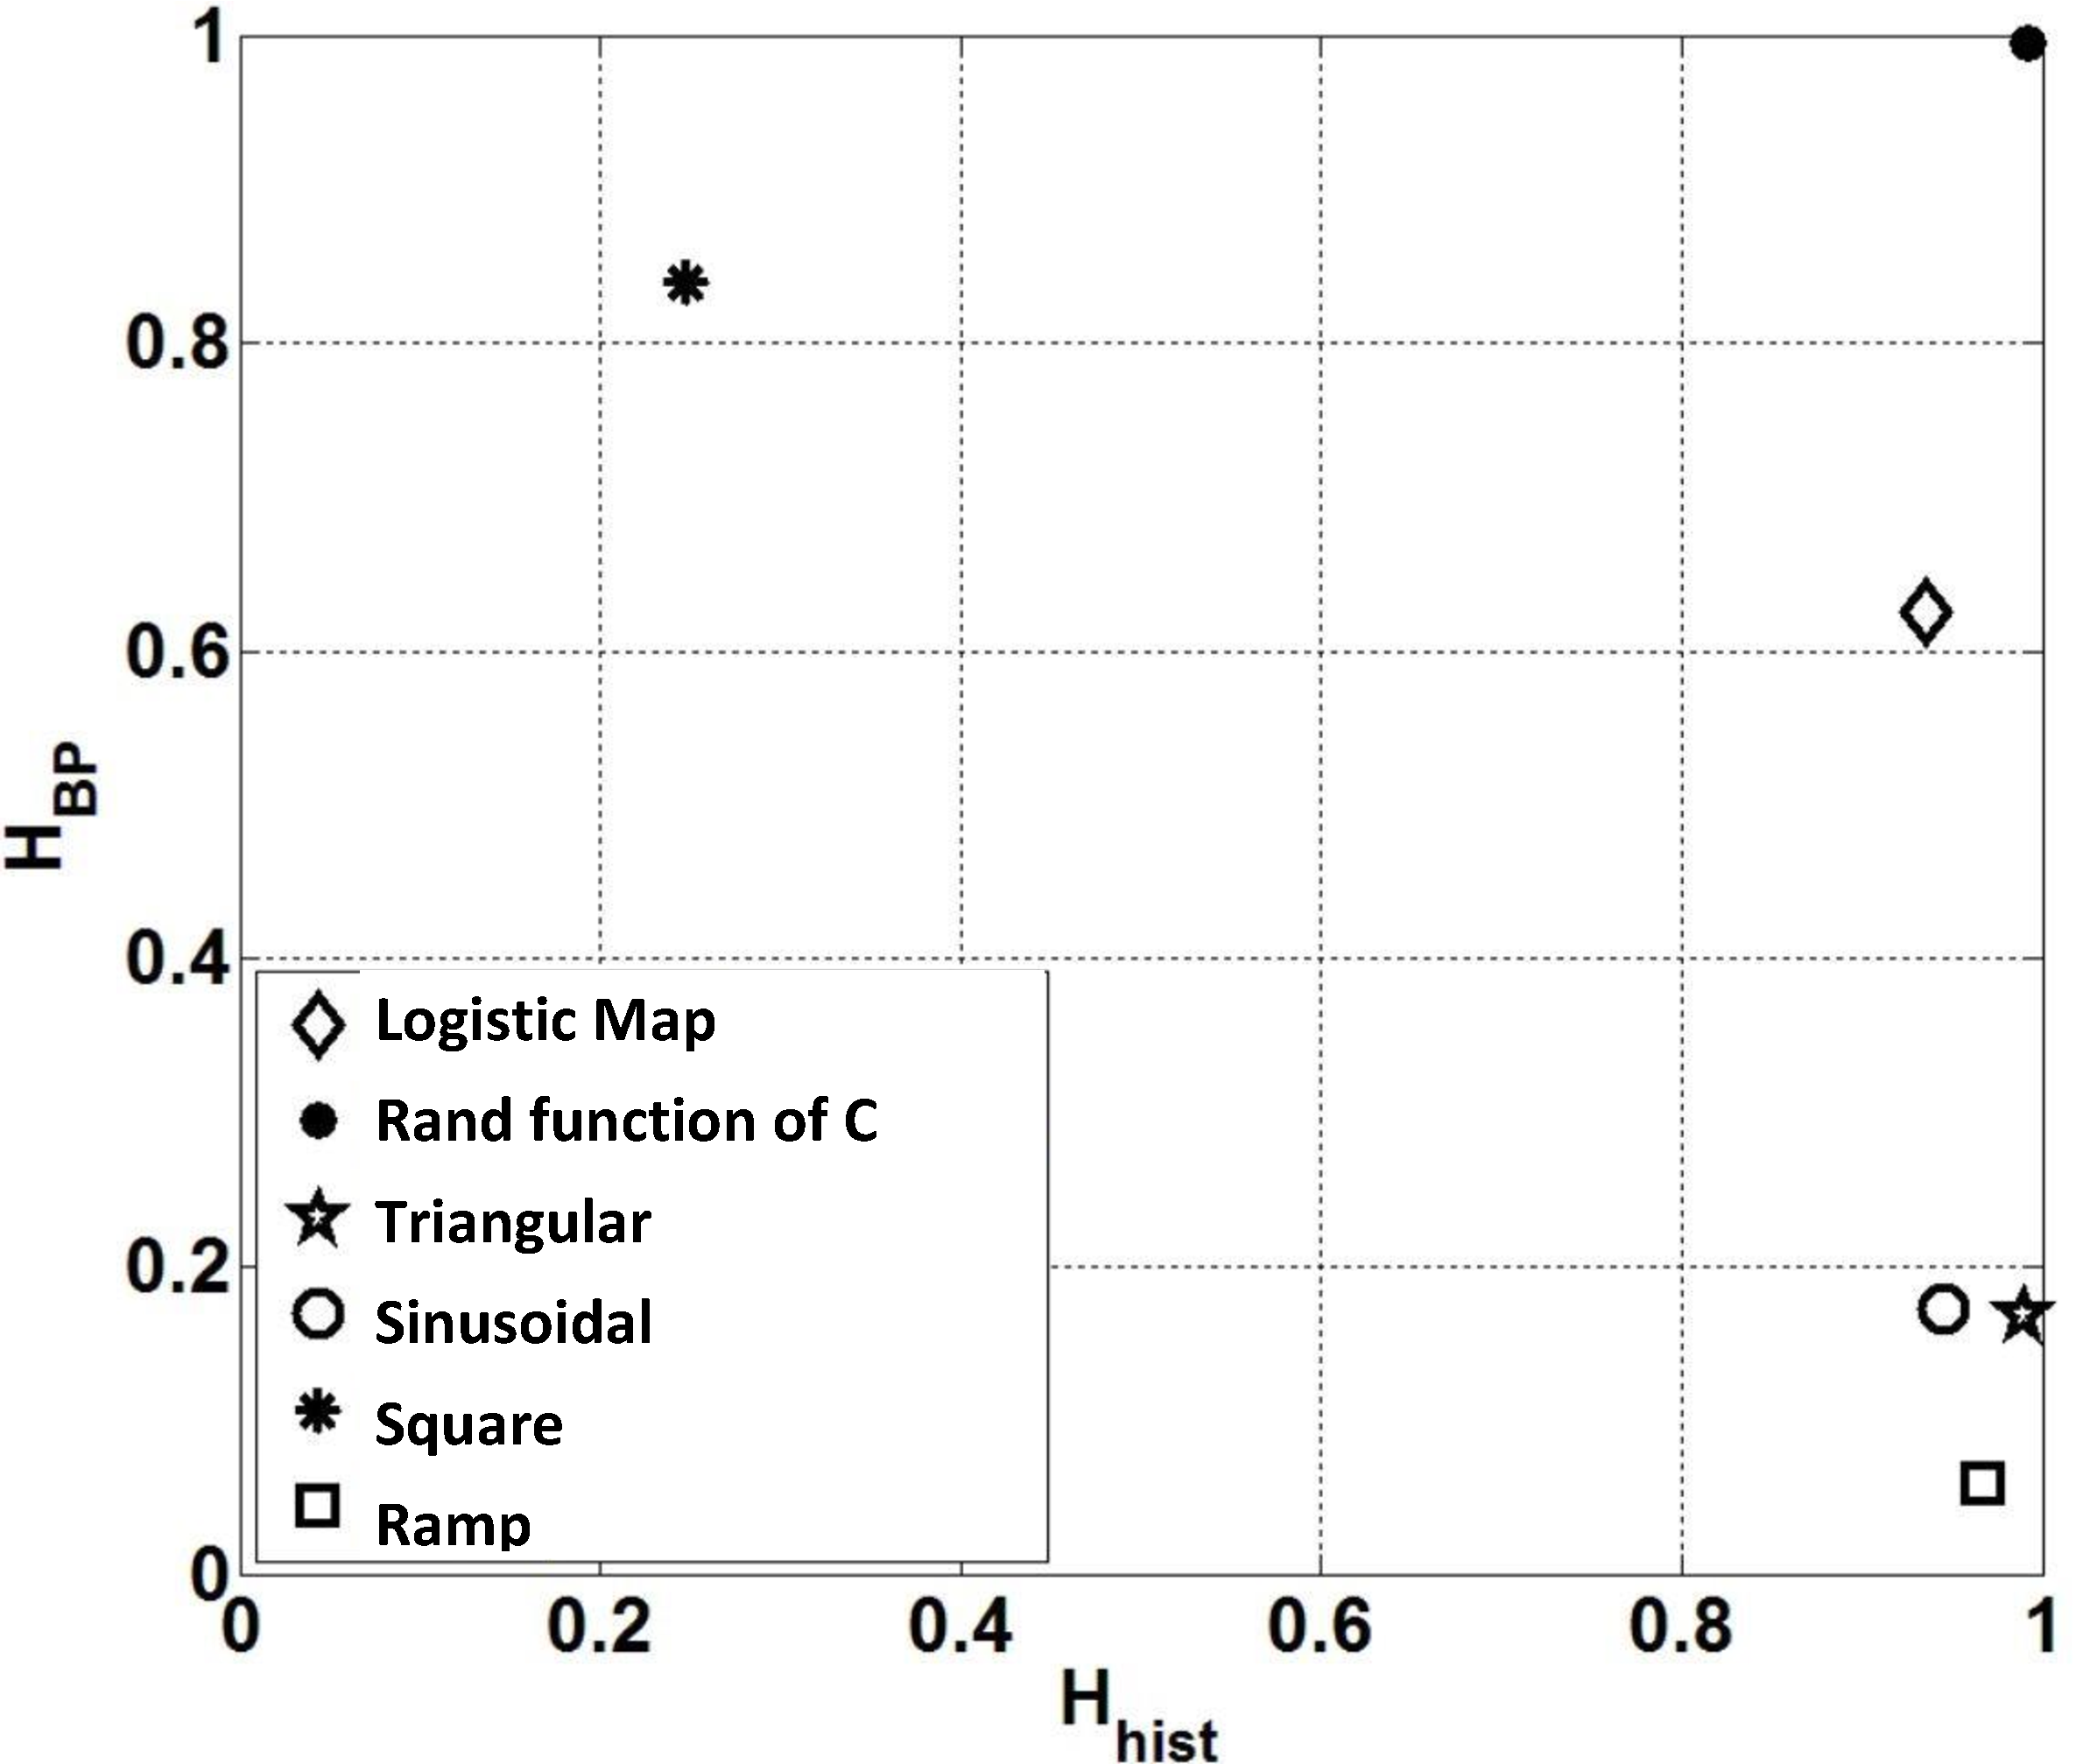
\includegraphics[height=0.26\textheight]{resultados_edit}
\caption{Measurement results.}\label{fig:resultados}
\end{figure}

Compilation results show the FPGA resources needed by the entire system and also the amount of memory occupied by the software running on the microcontroller. It is important to highlight that this is a rigid hardware implementation, i.e. the first circuit in the FPGA (microcontroller, peripheral, etc.) are configured and then the software is loaded on it.
The report returned after running the ``Place and Route" tool is shown in Fig. \ref{fig:hard}. 
It can be seen that the implementation uses 19\% of the FPGA logic resources, 21\% of the input-output cells and 28\% of the memory blocks.

The compilation report of the software part of the system is shown in Fig. \ref{fig:soft}. We can see that the non-volatile flash memory is 15.4\% occupied. 

On the other hand, of the $65536$ addresses the SRAM have available just $61440$ because some of this addresses are used by the APB bus, so the $76.7\%$ of the available memory is used.
%
\begin{figure}[htb]
\centering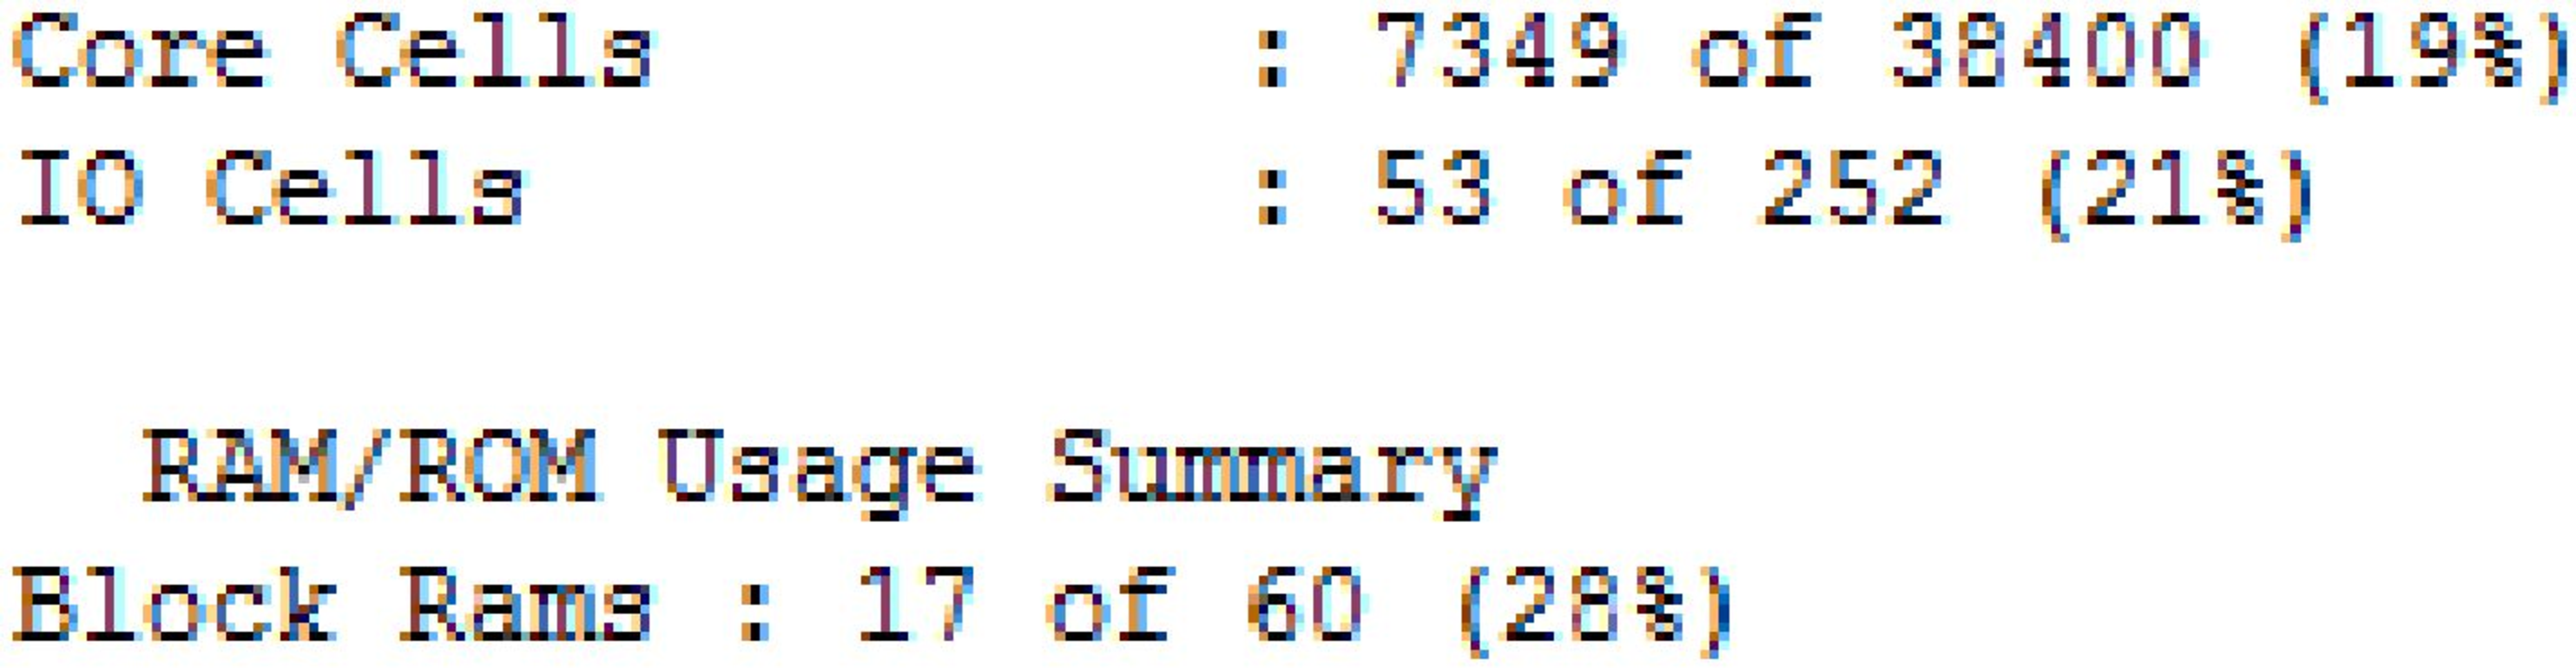
\includegraphics[scale=.13]{reporteHard}
\caption{Resources used by the system hardware.}\label{fig:hard}
\end{figure}

\begin{figure}[htb]
\centering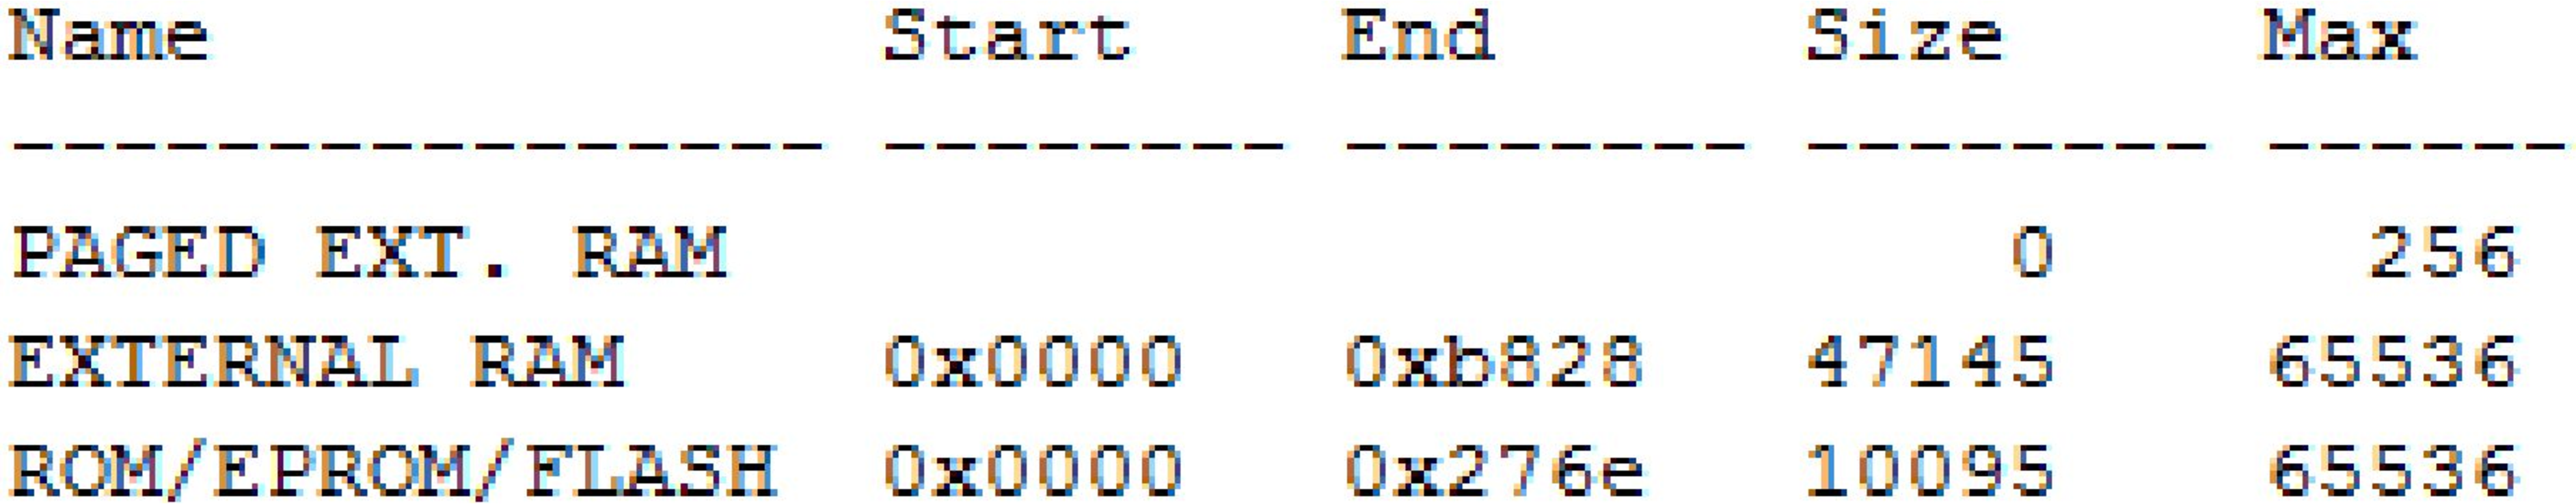
\includegraphics[scale=.13]{reporteSoft}
\caption{Resources used by the system software.}\label{fig:soft}
\end{figure}

\subsection{Discussion}
\label{sec:discusion}
%
The software had to be adapted to the microcontroller instantiated in the FPGA. 
The pattern program uses 64-bit floating point arithmetic (IEEE754-64~bits standard ) and uses the math.h library \cite{Mathe}.
For adapting the algorithm to be able to implement it in the  microcontroller that was instantiated in the FPGA, we had to reduce the number of bits employed. We used 32-bit floating point arithmetic (IEEE754-32~bits standard). The calculation of the logarithm function was also required, so it was implemented using the CORDIC algorithm. 
These differences make the output of the implemented system not to be equal to that of a program running on the PC, which we take as pattern program. Thus, these differences were measured, to have a dimension and determine whether the results are correct.

Table \ref{tabla} shows that the absolute error never exceeds the value $245E^{-6}$. This boundary indicates that there is a difference from the fifth decimal digit.

It can be seen in Fig. \ref{fig:resultados} that $H_{BP}$ and $H_{hist}$ quantifiers can clearly  difference between the statistical properties of the analyzed data.
Sinusoidal, Ramp and triangular signals have the highest values for $H_{hist}$ because the present all the possible values that the Analog-digital converter can generate.

However, the mixing of these signals are not good because they are periodic signals, so they are totally predictable, this is reflected by the small values of $H_{BP}$.
An interesting case to be analyzed is the square signal. The additive noise effect is specially marked in the areas where the value of the signal should be constant.

Two very narrow Gaussian curves appear around the ideal values of the $PDF_{hist}$, this does not affect too much the calculated value of $H_{hist}$, however for $PDF_{BP}$, the order pattern is derived directly from the noise, with a particular mean value, so the value of $H_{BP}$ will be higher than expected.

The signal generated by rand function of C has the best statistical properties being located at the point $\sim(1,1)$.

\subsection{Conclusions and future work}
\label{sec:conclusiones}
%
It was developed and implemented a system that allows a measurement with the proper precision of the causal and non-causal entropy of external analog signals from the outside of the FPGA and internal signals generated by code.
It was possible to measure signals and perform complex calculations with a small microcontroller as the 8051  instantiated in ACTEL AFS1500 FPGA. This first prototype meets the required specifications of accuracy and the quantity of resources established in the design. The following step will be to optimize the system regarding operating frequency and noise immunity.
It is expected that the system will allow modifying, at runtime, the sampling rate, so it would be adaptable to the input signal, with the upper limit of $500~Ks/s$ set by the ADC.

A threshold level should be added from which a value will be considered different from another, thus, the problem with the additive noise in the calculation of $H_{BP}$ will be solved.
The code for this system occupies $15.4\%$ of the total flash memory of the instantiated micro, so it will be possible to add software to implement other quantifiers and functionalities. As for the issue of the resources available in the FPGA, the logic cells used is $7349$, leaving almost $80\%$ of the available hardware resources to implement the systems under test, concurrently with the quantifiers.



%%%%%%%%%%%%%%%%%%%%%%%%%%%%%%%%%%%%%%%%%%%%%%%%%%%%%%%%%%%%%%%%%%%%%%%%%%%%%%%%%%%%%%%

\section{Measuring the Jitter of Ring Oscillators by means of Information Theory Quantifiers}

\subsection{Introduction}
\label{sec:intro}

%
\emph{Jitter} is any light deviation from the mean period of a presumed periodic signal. There are many physical examples where jitter is relevant. Some examples from different areas are:
(a) Stalberg et al \cite{Stalberg1971} found that the time interval between the two fibre action potentials of two muscle fibers -belonging to the same motor unit in the normal human muscles- shows a variability or jitter; (b) Mecozzi et al \cite{Mecozzi2001} detected timing and amplitude jitter in optical links using highly dispersed pulse transmission; (c) Derickson et al \cite{Derickson1991} made a comprehensive timing jitter comparison in the case of mode-locked semiconductor lasers; (d) the California and Carnegie Planet Search at Keck Observatory \cite{Wright2005} reported jitter in stars radial velocities; (e) Roberts \& Guillemin studied the delays  due to queueing in upstream multiplexing stages, in an Asynchronous Transfer Mode network (ATM); (f) Baron et al  \cite{Baron2012} considered the quality of the bunch clock signal of the Large Hadron Collider (LHC), in terms of jitter, a fundamental issue because it synchronizes all the electronics systems in the detector; (g) Marsalek et al analyzed the relationship between synaptic input and spike output jitter in individual neurons \cite{Marsalek1997}, etc. 

Furthermore, digital instruments are used in any modern experiment and the unavoidable jitter in the data acquisition systems produces uncertainties in time, and consequently in any spectrum determination. 

This paper is devoted to Ring Oscillators (\emph{RO}). Let us stress that in this particular application jitter is not always undesirable. Jitter is unwanted in applications that use the \emph{RO} as a clock generator \cite{Buedo1998,Beomsup1990,Hajimiri1999,Mandal2010,Gupta2011}. On the contrary random numbers generators \emph{RNG} using \emph{RO}'s, use jitter as the randomness source, \cite{Sunar2007,Wold2009}. Jitter also improves the Electromagnetic Compatibility as to distribute the clock frequency over a band, improving the Electromagnetic Compatibility (EMC) \cite{DeMicco2012}.

Determination of jitter in \emph{RO}'s has been studied in several papers: in \cite{McNeill1997} the study of three relevant time domain measures of jitter was presented. In \cite{Valtchanov2008} a model for jitter generation and distribution in \emph{RO}'s was proposed. In this seminal paper the authors brake up the jitter sources into deterministic and random (gaussian); furthermore each source is additionally classified into local or global. They demonstrate that the most important contributions are the local gaussian jitter and the global deterministic jitter and only the first one must be used as a randomness source of true random number generators (\emph{TRNG}'s). The same approach was used in \cite{Fischer2008,Valtchanov2010,Baudet2011,Jessa2011}. Lubicz et al. described a practical and efficient method to estimate the entropy rate of a \emph{TRNG} based on free running oscillators; they emphasized that their method does not require outputting and analyzing the clock signals with external equipment \cite{Lubicz2014} (a methodology that introduces extra jitter and distortion in the measured signal due to the data acquisition chain). 

Usually \emph{deterministic jitter} is the name given to any \emph{non-Gaussian jitter}. It is bounded and it is characterized by its peak to peak $\Delta_{pp}$ value. Random jitter is the name used for Gaussian jitter and it is unbounded and characterized by its RMS value. Sometimes deterministic periodic jitter appears. It has a \emph{period} that is the interval between two times of maximum (minimum) effect; the inverse of the time period is \emph{the frequency of the jitter}. Periodic jitter with jitter frequency below $10 Hz$ is usually named \emph{wander} and the name \emph{jitter} is reserved only to periodic jitter with frequencies at or above $10 Hz$. In communications, the \emph{total jitter} is $T = \Delta_{pp} + 2~n~R_{rms}$ where $n$ is a number between $6$ and $8$ related to the Bit Error Rate (\emph{BER}). 

\emph{RO}'s are one of the main building blocks in analog and digital integrated circuits and have been extensively used as \emph{on-chip oscillators} to generate clocks in high-speed circuits. Furthermore, \emph{RO}'s can be easily implemented in programmable digital circuits like \emph{FPGA}s. The main advantages of \emph{RO}'s over integrated \emph{LC} oscillators are their smaller chip area, their wider running range (that may be electrically tuned), and their lower power-consumption. 
 
Either one wants to use the \emph{RO} jitter or to eliminate it, jitter must be measured, and it is not a simple task. The main contribution of this paper is to provide a jitter measurement technique based on information theory quantifiers (\emph{ITQ}). We use a stochastic model which randomness is related to the jitter strength. Every proposed \emph{ITQ} used in this paper is based on an entropy, that is a Shannon functional of the probability distribution function (\emph{PDF}) assigned to the time series of the stochastic process. Disequilibrium and complexities may be used as well \cite{Amigo2005,Rosso2007b} but they do not represent an improvement in our case. In previous works \cite{DeMicco2008,DeMicco2009} we showed that many different \emph{PDF}'s can be assigned to the same data string. The best choice depends on the specific application. Two choices for the \emph{PDF} are used in this paper: the \emph{normalized histogram} and the \emph{ordering patterns histogram}. A representation plane is used to compare different situations. Once a \emph{PDF} is chosen, the Shannon Entropy is the basic functional that quantifies the uniformity of the \emph{PDF}. \emph{Normalized entropies}, \emph{differential entropies}, and \emph{rate entropies} are the other \emph{ITQ}'s evaluated. In our case \emph{differential entropies} give the best results and a \emph{differential entropy plane} is used to compare their sensitivity as a jitter measure.

%Experimental results for a \emph{RO} implemented in a \emph{Field Programmable Gate Array} (\emph{FPGA}) are also presented. 

Organization of the paper is as follows: section \ref{sec:jitter} describes jitter in \emph{RO}'s and explains how it is measured using random variables; section \ref{sec:quanti} details the evaluation of the considered \emph{ITQ}; section \ref{sec:resu} deals with the results using the proposed quantifiers. Finally, we present our conclusions in sec. \ref{sec:conclu}.

\subsection{Determination of jitter in \emph{RO}'s}
\label{sec:jitter}

There are two different situations concerning jitter in \emph{RO}'s: (a) for some applications it is enough to assure that jitter does not perturb the signal over an accepted limit. If this is the case the signal is observed on an oscilloscope with a mask over the display and it is enough to verify that the signal remains within tolerances; (b) in other cases an exact determination of jitter is required. One of these cases is the characterization of \emph{RO}'s, considered in this paper. 

Ideal \emph{RO}'s are composed of an odd number of inverters. Each inverter has a propagation time and consequently rising and falling edges separated by half-periods go through the inverters. If all the propagation times are constant the output of this \emph{ideal RO} is a square-wave with a discrete spectrum. But propagation times are not constant as there is jitter. Jitter distorts the delta like power spectrum as each $\delta$ is converted into a wider maximum. 

Let $T/2$ be the half-period of the \emph{ideal RO}. It is given by:
%
\begin{eqnarray}
\frac{T}{2}=k \sum_{i=1}^{k}d_i
\end{eqnarray}
%
where $k$ is the number of inverters and $d_i$ is the propagation time through the $i-$th inverter. When jitter exists, $d_i$ are random variables that can be modeled as:
%
\begin{eqnarray}
d_i=D_i+ \bigtriangleup d_i
\end{eqnarray}
%
where $D_i$ is the mean value of $d_i$ with nominal source voltage level and normal temperature, and $\bigtriangleup d_i$ is the delay variation produced by both local physical events and global changes in the device working conditions (as VCC, temperature, etc.). Then jitter in \emph{RO}'s is evidenced by the random displacement of the trailing (falling) edges from their otherwise perfectly periodic location. The direct measurement of this displacement has two main problems: (a) requires a very high-frequency instrument, because time resolution is limited by the sampling period $T_s$; (b) this technique introduces extra jitter and distortions in the measured signal coming from the data acquisition chain. Then it is more convenient to use \emph{indirect measurements}, by means of auxiliary random variables related to statistical properties related with jitter to measure jitter with minimal disturbance \cite{Lubicz2014}. The general procedure is as follow:
\begin{enumerate}
\label{list:altrenew}
\item Sample the output with sampling period $T_s$ to get a binary time series. 
In the ideal case of \emph{no-jitter} the output is a \emph{continuous and perfectly periodic square wave} with period $T$. Then it is possible to adjust $T_s$ to make $T/2=m~T_s$ with $m\in N^+$. The binary time series will be periodic with $m$ \emph{1}'s followed by $m$ \emph{0}'s. When jitter is present the binary series is not periodic but stochastic. This stochastic model is known as \emph{alternating renewal process}.
\item Many different randomness quantifiers may be used to characterize the stochastic model associated with the measured jitter. In this paper, we propose the use of \emph{ITQ}'s. 
\end{enumerate}
%
Note that jitter is accumulative and two basic situations arise: (a) if the jitter introduced by each stage is assumed to be totally independent of the jitter introduced by other stages, it means $\sigma_T^2=m*\sigma_s^2$, where $\sigma_s$ is the jitter of each sample, and it is supposed that all samples have jitter with the same normal distribution; (b) if jitter sources are totally correlated with one another then $\sigma_T=m*\sigma_s$. 

\subsection{Information Theory Quantifiers}
\label{sec:quanti}

\subsubsection{Time series and probability distribution functions }
\label{subsec:probabilities}

Shannon Entropy is the functional of $P$ more frequently used in the literature (there are other functionals, like statistical complexity, disequilibrium, etc.). An important issue is $P$ itself is not a uniquely defined object and do exist several approaches to ``associate'' a given $P$ with a given time series. Just to mention some extraction procedures frequently used in the literature: {\it a)\/} time series histogram \cite{Martin2004}, {\it b)\/} binary symbolic-dynamics \cite{Mischaikow1999}, {\it c)\/} Fourier analysis \cite{Powell1979}, {\it d)\/} wavelet transform \cite{Blanco1998,Rosso2001}, {\it e)\/} partition \emph{PDF} \cite{Ebeling2001}, {\it f)\/} permutation \emph{PDF} \cite{Pompe2002,Keller2005}, {\it g)\/} discrete \emph{PDF} \cite{Amigo2007}, etc. There is ample liberty to choose among them and the specific application must be analyzed to make a good choice.

The general procedure to assign $P$ to a given time series consists in the following steps:
\begin{itemize}
\item (a) define an alphabet $\mathfrak A=\{\mathrm{s}_j, j=1,...m\}$ 
\item \label{list:pdf} (b) convert the time series $X=\{x_i, i=1,...\}$ into a \emph{symbolic sequence} $A=\{a_i, a_i\in \mathfrak A\}$. 
\item (c) $P$ is given by the relative frequencies of the symbols: $P=\{p_j, j=1,...,m\}$ in the symbolic sequence $A$, where $p_j$ is the relative frequency of symbol ${\mathrm{s}_j}$. 
\end{itemize}
%
$P$ may be \emph{non-causal} or \emph{causal} \cite{DeMicco2008} depending on step b. $P$ is \emph{non-causal} when one symbol $\mathrm{s}_j\in \mathfrak A$ is assigned to each value $x_i\in X$. For example, the usual histogram technique used for time series of real numbers corresponds to this kind of assignment. Of course, in this method the temporal order of the time-series plays no role, and consequently the resulting $P$ will not have any \emph{causal information} and the \emph{symbolic sequence} may be simply regarded as a \emph{coarse-grained} description of $X$ \cite{DeMicco2008}. It is also possible to group $W$ consecutive values of the time series -a \emph{trajectory} of length $W$- and assign one symbol to the group. Note that this procedure is equivalent to first assign a symbol to each value of the time series, then group $W$ symbols into a \emph{word} and finally construct a new alphabet consisting of words. If the original alphabet has $m$ elements, there will be $m^W$ possible words and one of this words will be assigned to the \emph{trajectory} of $W$ elements. $P$ is given by the relative frequencies of all the possible words. Here $P$ depends on the temporal order of $X$ and consequently we call it a \emph{causal} $P$. It is interesting to note that a \emph{causal} $P$ has information about statistics and also about temporal ordering of $X$. If a \emph{non-causal} $P$ is used instead, the analysis must be complemented with the evaluation of the Fourier transform, or the autocorrelation function of $X$, to recover the information about temporal ordering.

Let us stress even more the difference between a \emph{non-causal} and a \emph{causal} $P$ by means of the following simple example. Let $X=\{x_i,~i=1,2,...\}$ be a time series generated by $randn$ (Matlab's$^\copyright$ function); let $Y=\{y_i,~i=1,2,...\}$ be the resulting series after a sorting process made by $sort$ (Matlab's$^\copyright$ function). Figs. \ref{fig:causal_nocausal}.a and \ref{fig:causal_nocausal}.b show the time series. One noncausal $P$ is the normalized histogram, and $P(X)$ is identical to $P(Y)$ as Figures \ref{fig:causal_nocausal}.c and \ref{fig:causal_nocausal}.d reveal. One causal $P$ may be obtained by the Bandt \& Pompe procedure (for details about its determination see below) and Figs. \ref{fig:causal_nocausal}.e and \ref{fig:causal_nocausal}.f show that $P(X)$ and $P(Y)$ are completely different: $P(X)$ is almost uniform, reflecting $X$ is randomly ordered, but $P(Y)$ has a delta-like shape, as far as $Y$ is monotone increasing and only one ordering pattern is present.

\begin{figure}
\center
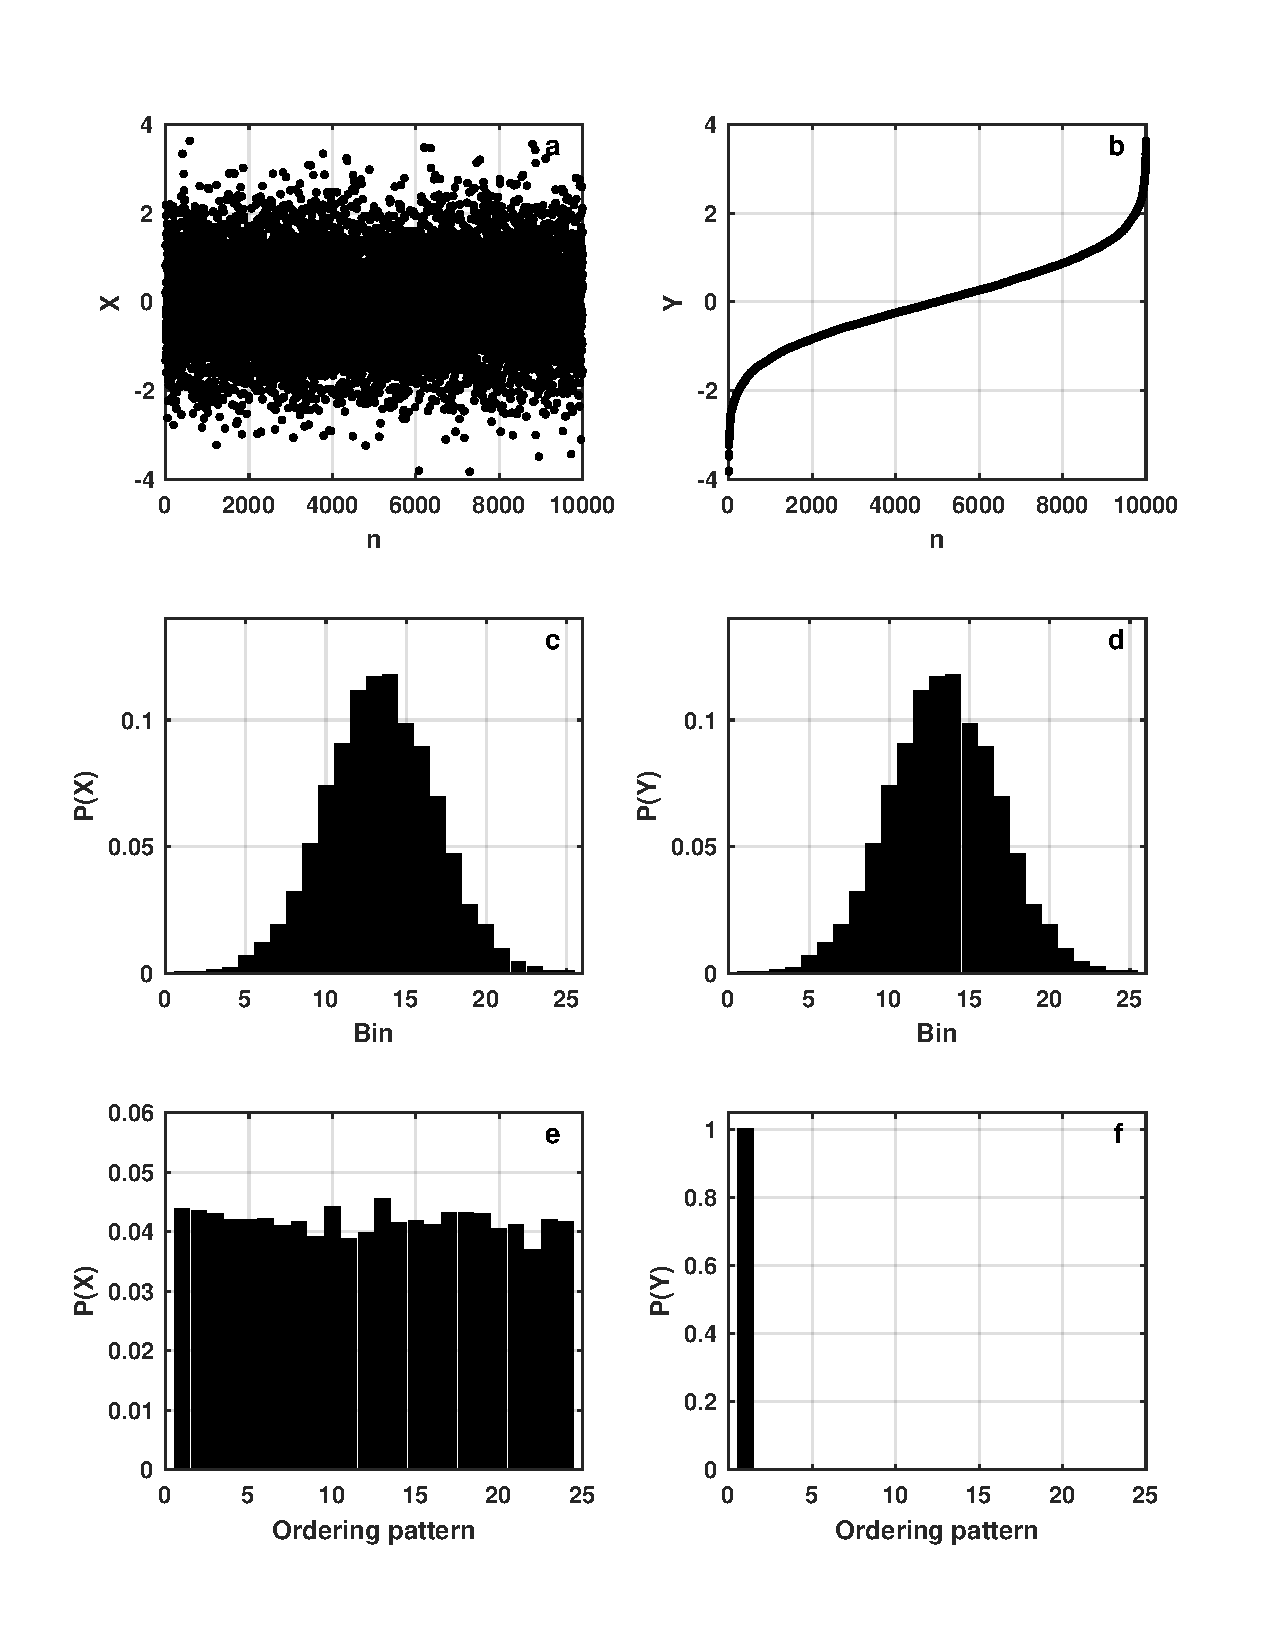
\includegraphics[width=1\textwidth]{causal_nocausal}
\caption{(see text) Time series $X$ obtained by using function \emph{randn} (a), its sorted version $Y$ (b) and their causal (c, d) and non-causal histograms (e, f).}
\label{fig:causal_nocausal}
\end{figure}

Let us consider now the case of sampled digital signals like as sampled \emph{RO}'s outputs are. Time series $X$ is binary and has a natural alphabet with two symbols
$\mathfrak{A}=\{0,1\}$. The Shannon entropy of this alphabet is usually known as \emph{Binary Entropy} $S_2$. Suppose $W$ consecutive bits of $X$ are grouped into \emph{a word}, that is the decimal number $w_i$ between $0$ and $2^W-1$; consider these decimal numbers as the symbols of the new alphabet and let $Z=\{w_i,~i=1,2,...\}$ be the new symbolic series. $S_W$ is the entropy of $P_{hist}(Z)$ where subscript \emph{hist} is for histogram; $S_W$ is also known as \emph{Block Entropy} of the binary time series $X$. Furthermore, if $D$ consecutive decimal numbers $w_i$ are grouped again and the $D!$ permutation patterns are considered as symbols of the new alphabet, we get a new $P_{BP}(Z)$, given by the relative frequencies of the permutation patterns. The entropy is $S^{(D)}_{BP}$, the \emph{Bandt \& Pompe entropy} \cite{Pompe2002} of the binary time series.
All the above-mentioned entropies are given by the same Shannon famous formula:
%
\begin{equation}
S~=~-~\sum_{j=1}^{m}{p_j~log(p_j)}, 
\end{equation}
%
and the only difference between them is the $P$ assigned to the time series. In this paper
$log$ means \emph{base $2$ logarithm}.

In this paper, we use a causal $P$ determined with the Bandt \& Pompe procedure. This procedure has been described in detail and successfully used in a number of papers concerning pseudo random number generation, system classifications, etc. \cite{Amigo2005,Rosso2007b,DeMicco2008,DeMicco2009,Amigo2010,Rosso2008}.
Let us summarize the basic procedure applied to our specific case:
\begin{itemize}
\item let $Z=\{w_i,~i=1,2,...\}$ be a numerical time series (in our case $W$ bits decimal numbers) series;
\item choose an embedding dimension $D~>~1$
\item assign to each $w_i$ a $D$-dimensional vector of previous $i, i-1,\cdots,i-(D-1)$:

\begin{equation}
\label{eq:vectores}
(s)\mapsto \left(w_{i-(D-1)},w_{i-(D-2)},\cdots,w_{i-1},w_{i}\right)
\end{equation}

Clearly, the greater the $D-$value, the more information about ``the past" is incorporated into these vectors. 
\item look for \emph{ordinal patterns} of length $D$ \cite{Pompe2002,Keller2003,Keller2005}. By ``ordinal pattern" related to position $i$ we mean the permutation $\pi=(r_0, r_1, \cdots,r_{D-1})$ of $(0, 1, \cdots, D-1)$ defined by

\begin{equation}
\label{eq:permuta}
w_{i-r_{D-1}}\le w_{i-r_{D-2}}\le\cdots\le w_{i-r_{1}}\le a_{i-r_0}
\end{equation}
\item In order to get a unique result consider that $r_j <r_{j-1}$ if $x_{i-r_{j}}=x_{i-r_{j-1}}$. 
\item Thus for all the $D!$ possible permutations $\pi$ of order $D$ is the probability distribution $P=\{p(\pi)\}$ defined by

\begin{equation}
\label{eq:frequ}
p(\pi)~=~ \frac{\sharp \{s|s\leq M-D+1; i \quad \texttt{has type}~\pi\}}{M-D+1}
\end{equation}

In the last expression, the symbol $\sharp$ stands for ``number" and corresponds to the number assigned to the permutation using the lexicographic order . 
\end{itemize}

The main advantages of the Bandt \&Pompe method are {\it a)\/} its simplicity, {\it b)\/} the extremely fast nature of the pertinent calculation-process, {\it c)\/} its robustness in the presence of observational and dynamical noise, and {\it d)\/} its invariance with respect to nonlinear monotonous transformations. The Bandt \&Pompe methodology is not restricted to time series representative of low dimensional dynamical systems but can be applied to any type of time series (regular, chaotic, noisy, or reality based), with a very weak stationary assumption (for $k~=~D$, the probability for $a_i < a_{i+k}$ should not depend on $i$ \cite{Pompe2002}).

Let us stress some important issues involved in the calculations of the above-mentioned entropies:
\begin{enumerate}
\item The binary entropy $S_2$ is noncasual while both, the block entropy $S_W$ and the Bandt \& Pompe entropy $S^{(D)}_{BP}$, are causal. 
\item The block entropy $S_W$ takes into account correlations between $W$ consecutive bits. Bandt\& Pompe entropy $S^{(D)}_{BP}$ takes into account correlations between $D$ consecutive $W$-length words.
Both grouping procedures (decimal numbers of $W$ bits and permutation patterns of $D$ decimal numbers) may be done with or without superposition. The number of data required for good statistics is different depending the grouping procedures are made with superposition or not.
\item For $S_W$ there is only one grouping process ($W$ bits are grouped to obtain a decimal numbers time series $Y$). Let us define $\alpha$ as a statistical quality parameter, given by the quotient between the number of elements in the symbolic time series $Y$ and the number of symbols in the alphabet. In this paper we will not accept $\alpha~<~10$. 

Obviously the quality factor $\alpha$ increases with the length of the time series:
%
\begin{enumerate}
\item If the grouping of $W$ bits is made with superposition, two consecutive $W$-length words share $W-2$ bits. Consequently starting with a file with a length of $N$-bits we get $N-W+1$ words. Furthermore, there are $2^W$ symbols in the alphabet and $\alpha=(N-W+1)/(2^W)$. 
\item If $S_W$ is evaluated without superposition the number of $W$-length words is $floor~\{N/W\}$ and the quality parameter becomes $\alpha=floor~\{N/W\}/(2^W)$. For $N\gg W$ the statistical quality factor is $W$ times lower that the one with superposition.
\end{enumerate}

\item In the case of $S^{(D)}_{BP}$, there are two grouping processes involved. 
\begin{enumerate}
\item If both grouping processes are made with superposition we get $N-W-D+2$ elements starting with a file $N$-bits length, and the quality factor is $\alpha=(N-W-D+2)/D!)$. In this case $S^{(D)}_{BP}$ takes into account the correlations between $W+D$ consecutive bits. 
\item If the grouping process of $W$ bits is made without superposition but the grouping of $D$ decimal numbers is made with superposition we get $floor\{N/W\}-D+1$ elements and the statistical quality parameter is $\alpha=(floor\{N/W\}-D+1)/D!$. In this case $S^{(D)}_{BP}$ will include correlations between $WD$ consecutive bits. 
\item If the grouping process of $W$ bits is made with superposition and the grouping of $D$ decimal numbers is made without superposition we get $floor\{(N-W+1)/D\}$ elements starting from a file with $N$ bits.The statistical quality factor is $\alpha=floor\{(N-W+1)/D\}/D!$ and $S^{(D)}_{BP}$ takes into account correlations between $W+D-1$ bits.
\item If both grouping processes are made without superposition we get $floor\{floor\{N/W\}/D\}$ elements starting from a $N$-bits length file. The statistical quality factor is $\alpha=floor\{floor\{N/W\}/D\}/D!$ and $S^{(D)}_{BP}$ takes into account correlations between $WD$ consecutive bits.
\end{enumerate}
\end{enumerate} 

\subsubsection{Additional quantifiers}
\label{subsec:addquanti}

The Shannon Entropy $S(P)$ is the startpoint for other quantifiers:
\begin{enumerate}
\item Normalized entropy $H(P)$: it is the Shannon Entropy divided by its maximum value. For example, if we use $S_2$ (see above), the maximum entropy is obtained for equiprobability between two symbols. Its value is $S_{max}=-1/2 log(1/2)-1/2 log(1/2)=log(2)=1$; then, the normalized entropy is $H_2=S_2$. If we use $S_W$ the equiprobability between the $2^W$ possible words ($W$-bits decimal numbers) produces $S_{max}=W$ and $H_W=S_W/W$. Finally for $S^{(D)}_{BP}$ the equiprobability between the $D!$ ordinal patterns produces $S_{max}= log(D!)$ and $H^{(D)}_{BP}=S^D_{BP}/log(D!)$.
\item Differential or conditional entropies $h$ and $h^*$ are:
\begin{eqnarray}
h~=~S_{W+1}-S_W\\
h^*~=~S_{BP}^{(D+1)}-S_{BP}^{(D)}
\end{eqnarray}
In the above expressions $W=1,2,...$ and $D=2,3,...$, $S_0=0$ and $S_{BP}^{(1)}=0$. These differential or conditional entropies give the average amount of information required to predict the $(W+1)$ (or $(D+1)$) symbol, given the preceding $W$ (or $D$) symbols.
\item Finally the \emph{rate entropies} $h_0$ and $h_0^*$ are given by:

\begin{eqnarray}
h_0=\lim\limits_{W\rightarrow \infty} h=\lim\limits_{W\rightarrow \infty}{S_{W}/W }\\
h^*_0= \lim\limits_{D\rightarrow \infty} h^*=\lim\limits_{D\rightarrow \infty}{S^{(D)}_{BP}/(D-1)}
\end{eqnarray}

\end{enumerate}

Let us tell in advance that we shall show in section \ref{sec:resu} that quantifiers $S_W$, $S^{(D)}_{BP}$ , $H_W$ and $H^{(D)}_{BP}$ are dependent on parameters $W$ and $D$. This is a drawback if we want to use them as jitter measures. On the other hand, the estimators $h$ and $h^*$ of the \emph{rate entropies} $h_0$ and $h^*_0$ \cite{Ebeling2001,Amigo2005} instead, are independent of $W$ and $D$ and we will show in Section \ref{sec:resu} that in the case of sampled \emph{RO}'s they also present a minimum for the correct sampling ratio making them good measure of the quality of both \emph{RO}'s and \emph{PRNG}'s derived from them. 

\subsection{Results}
\label{sec:resu}

An evenly sampled output of a jitter-less \emph{RO} was simulated with Matlab\textsuperscript{\copyright} and an output file with a length of $N_b=7,000,000$ of bits was generated. A set of a hundred values of the sampling ratio $r= T_s/T\in[6.5,9.5]$, was explored (where $T_s$ is the sampling period and $T$ is the \emph{RO}  output period). Jitter with a normal distribution and a set with different values of variance $\sigma_s$ (see below) were added to the original file. Our method emulates the real process of sampling the noisy output of a real \emph{RO}; the detailed code is published in Mathworks\cite{MathworksMaxi}.

For each value of $\sigma_s$, ten surrogates (each one with a different random initial condition) were generated and new files with $N_b$ bits each were stored. It was assumed that jitter of individual samples is independent, normal distributed random variables, with zero mean value and variance $\sigma_i=\sigma_s$. Consequently, the variance of the accumulated jitter over one period $T$ is given by $\sigma^2_T=r \sigma^2_s$ \cite{Valtchanov2008}. The values considered  are $\sigma_T=\{0,$ $0.001,$ $0.002,$ $0.003,$ $0.004,$ $0.005,$ $0.007,$ $0.01,$ $0.02,$ $0.02,$ $0.04,$ $0.05,$ $0.07,$ $0.1\}$.

For each file all the quantifiers defined in \ref{sec:quanti} were evaluated for $D\in[2,10]$ and $W\in[1,26]$. The details about evaluation, advantages and drawbacks of each quantifier are reported in section \ref{sec:quanti}: they are $S_W$, $S^{(D)}_{BP}$, $H_{W}$, $H^{(D)}_{BP}$, $h$ and $h^*$.  Let us only show here the  more relevant results  to show the reason the last two quantifiers ($h$ and $h^*$) are the best ones.

\begin{itemize}
\item In the case of normalized entropy $H_{W}$, it strongly depends on $W$. Furthermore the analysis of $H_{W}$ as a function of $r$ shows that it does not allow to determine an optimum value of the sampling ratio $r$ (see Fig. \ref{fig:H_W_rCS}). This is an important issue if the quantifiers are going to be used for experimental setups. 
\item In the case of the normalized Bandt \& Pompe entropy $H^{(D)}_{BP}$, a strong dependence on the embedding dimension $D$ is additionally present. Again it is not easy to determine the optimum value of $r$ from the analysis of this parameter as a function of $r$  (see Fig. \ref{fig:HBP_W_rSS}). 
\item A similar behavior appears in all the other functionals related with these two entropies. 
In summary, our results show that  both $ h$ y $h^*$ are independent of any arbitrary parameter used in their statistical determination.  These two quantifiers have also been considered in two excellent articles \cite{Amigo2006,Ebeling2001}. 
\end{itemize}
%
\begin{figure}
\center
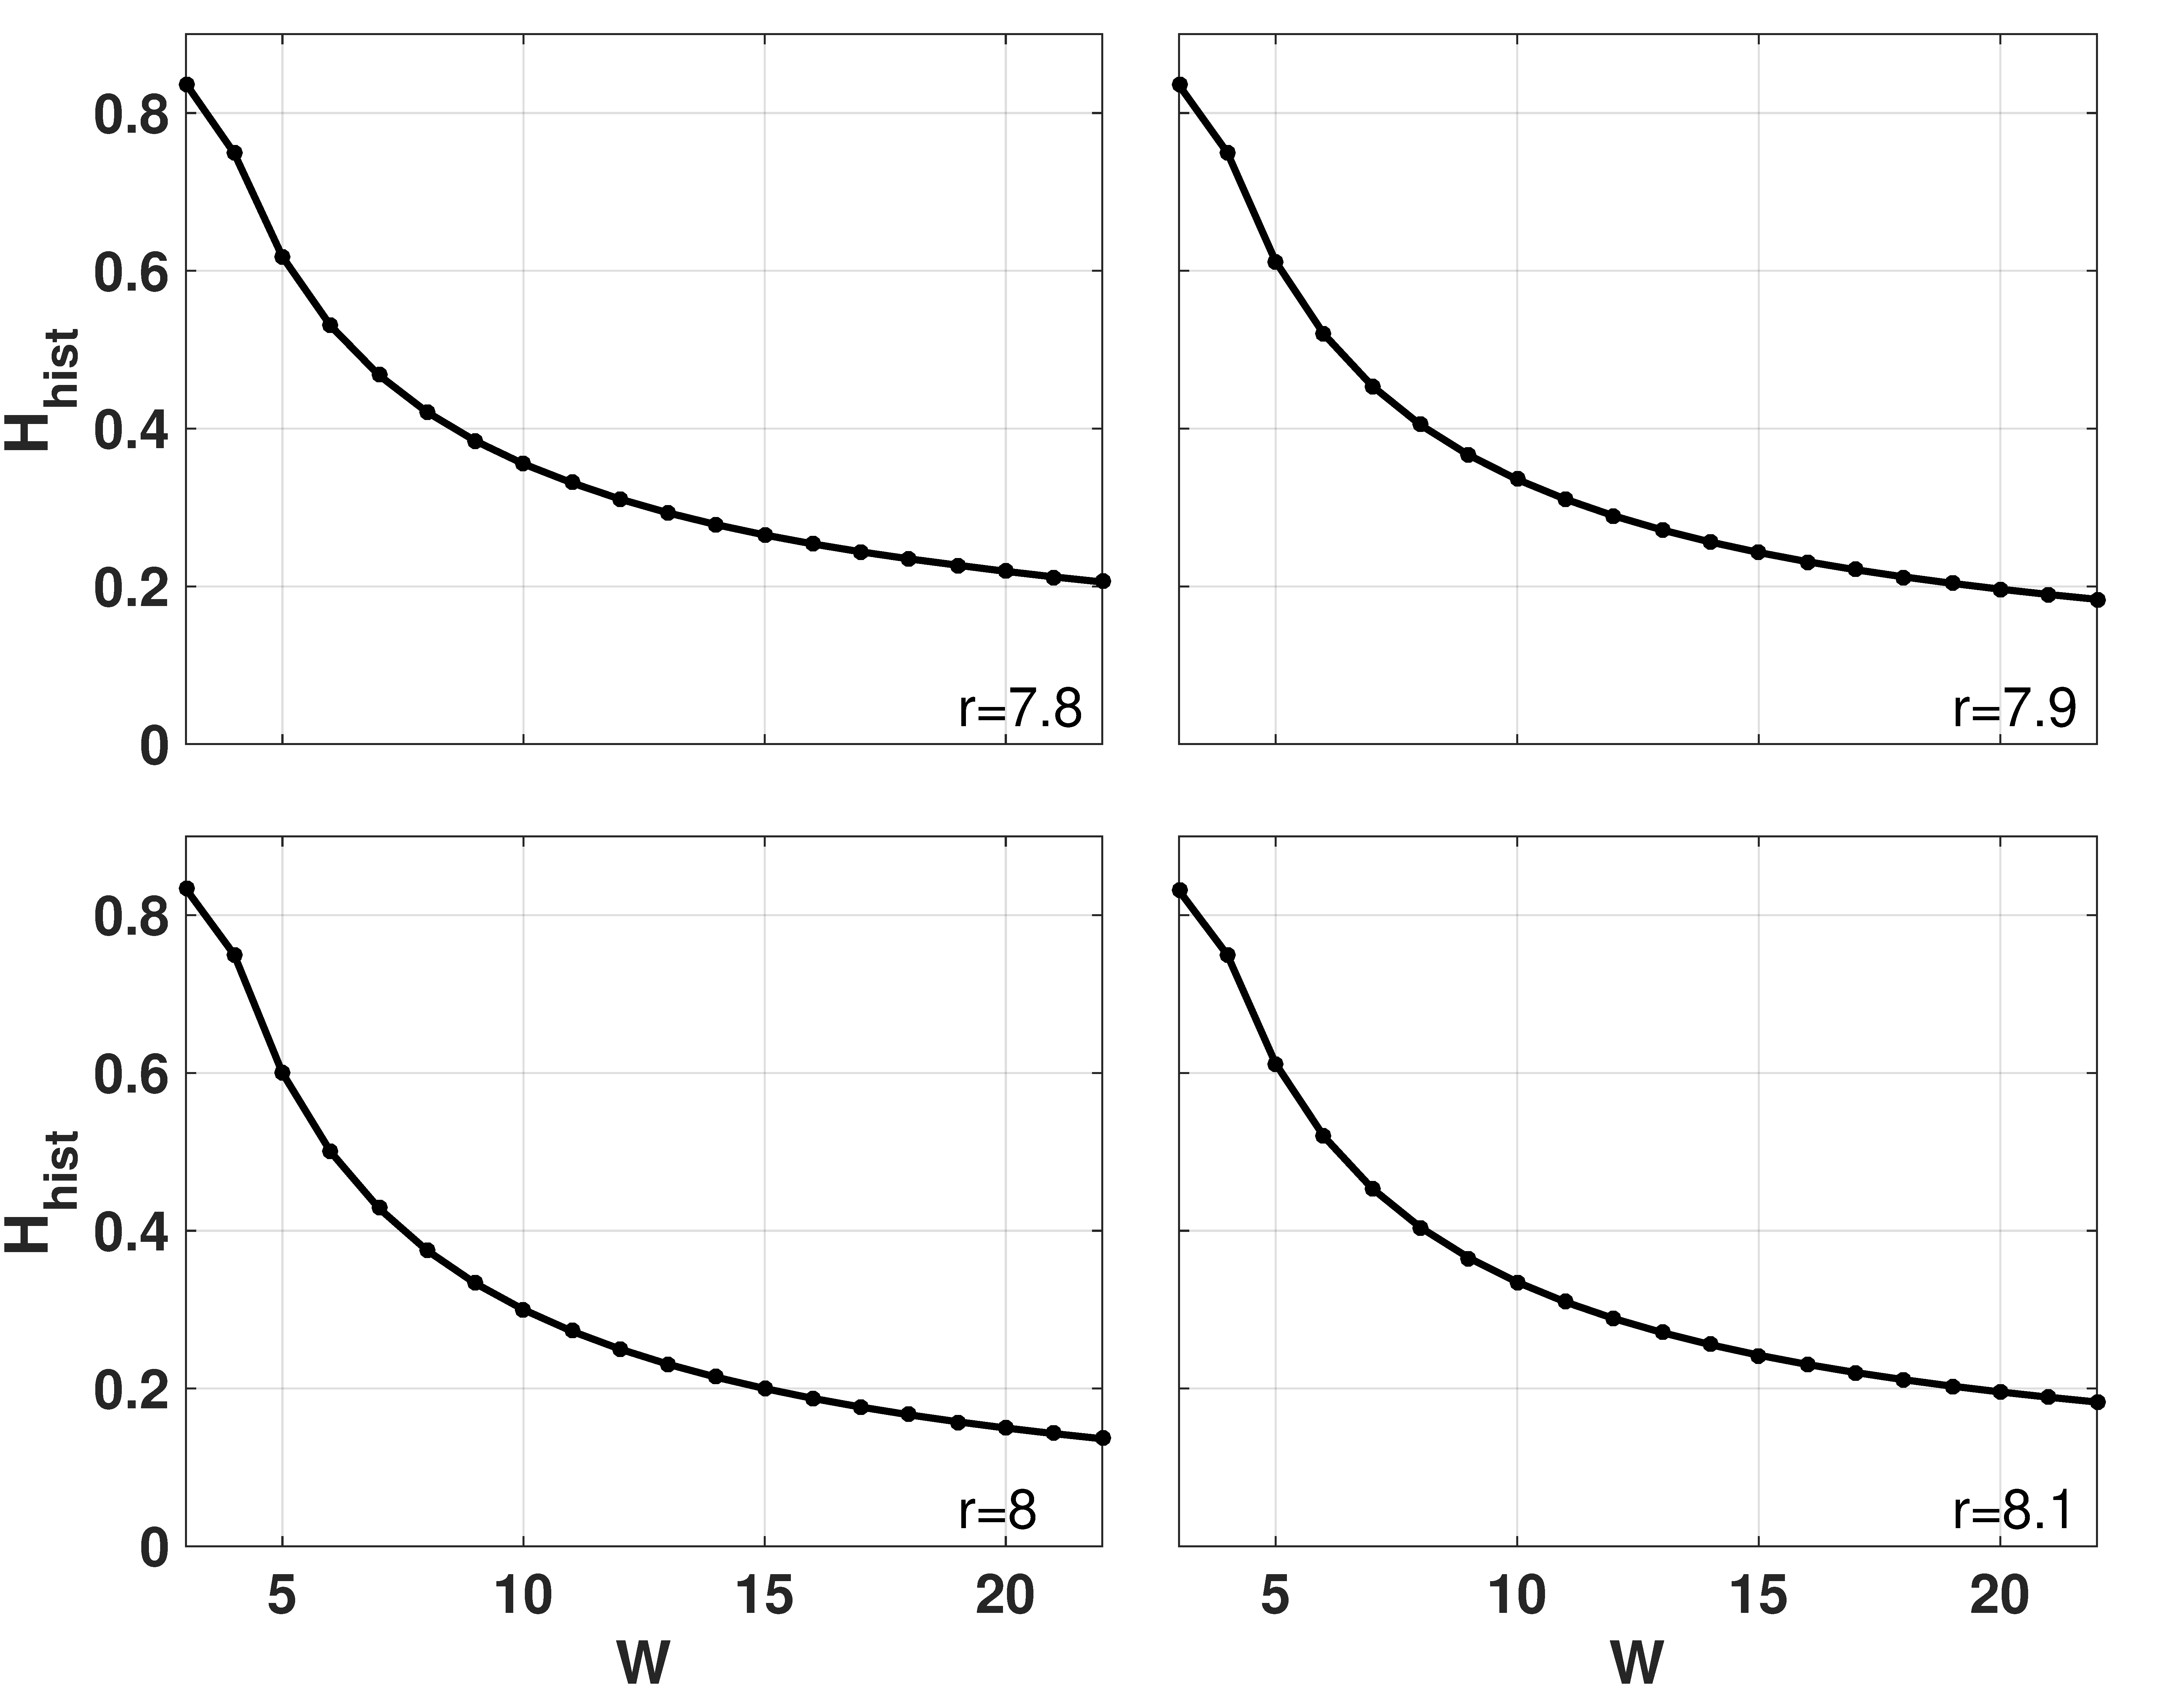
\includegraphics[width=0.8\textwidth]{H_W_rCS}
\caption{Normalized entropy $H_W$ as a function of $W$ for a jitter-less \emph{RO} sampled with different values of $r$.}
\label{fig:H_W_rCS}
\end{figure}
%
\begin{figure}
\center
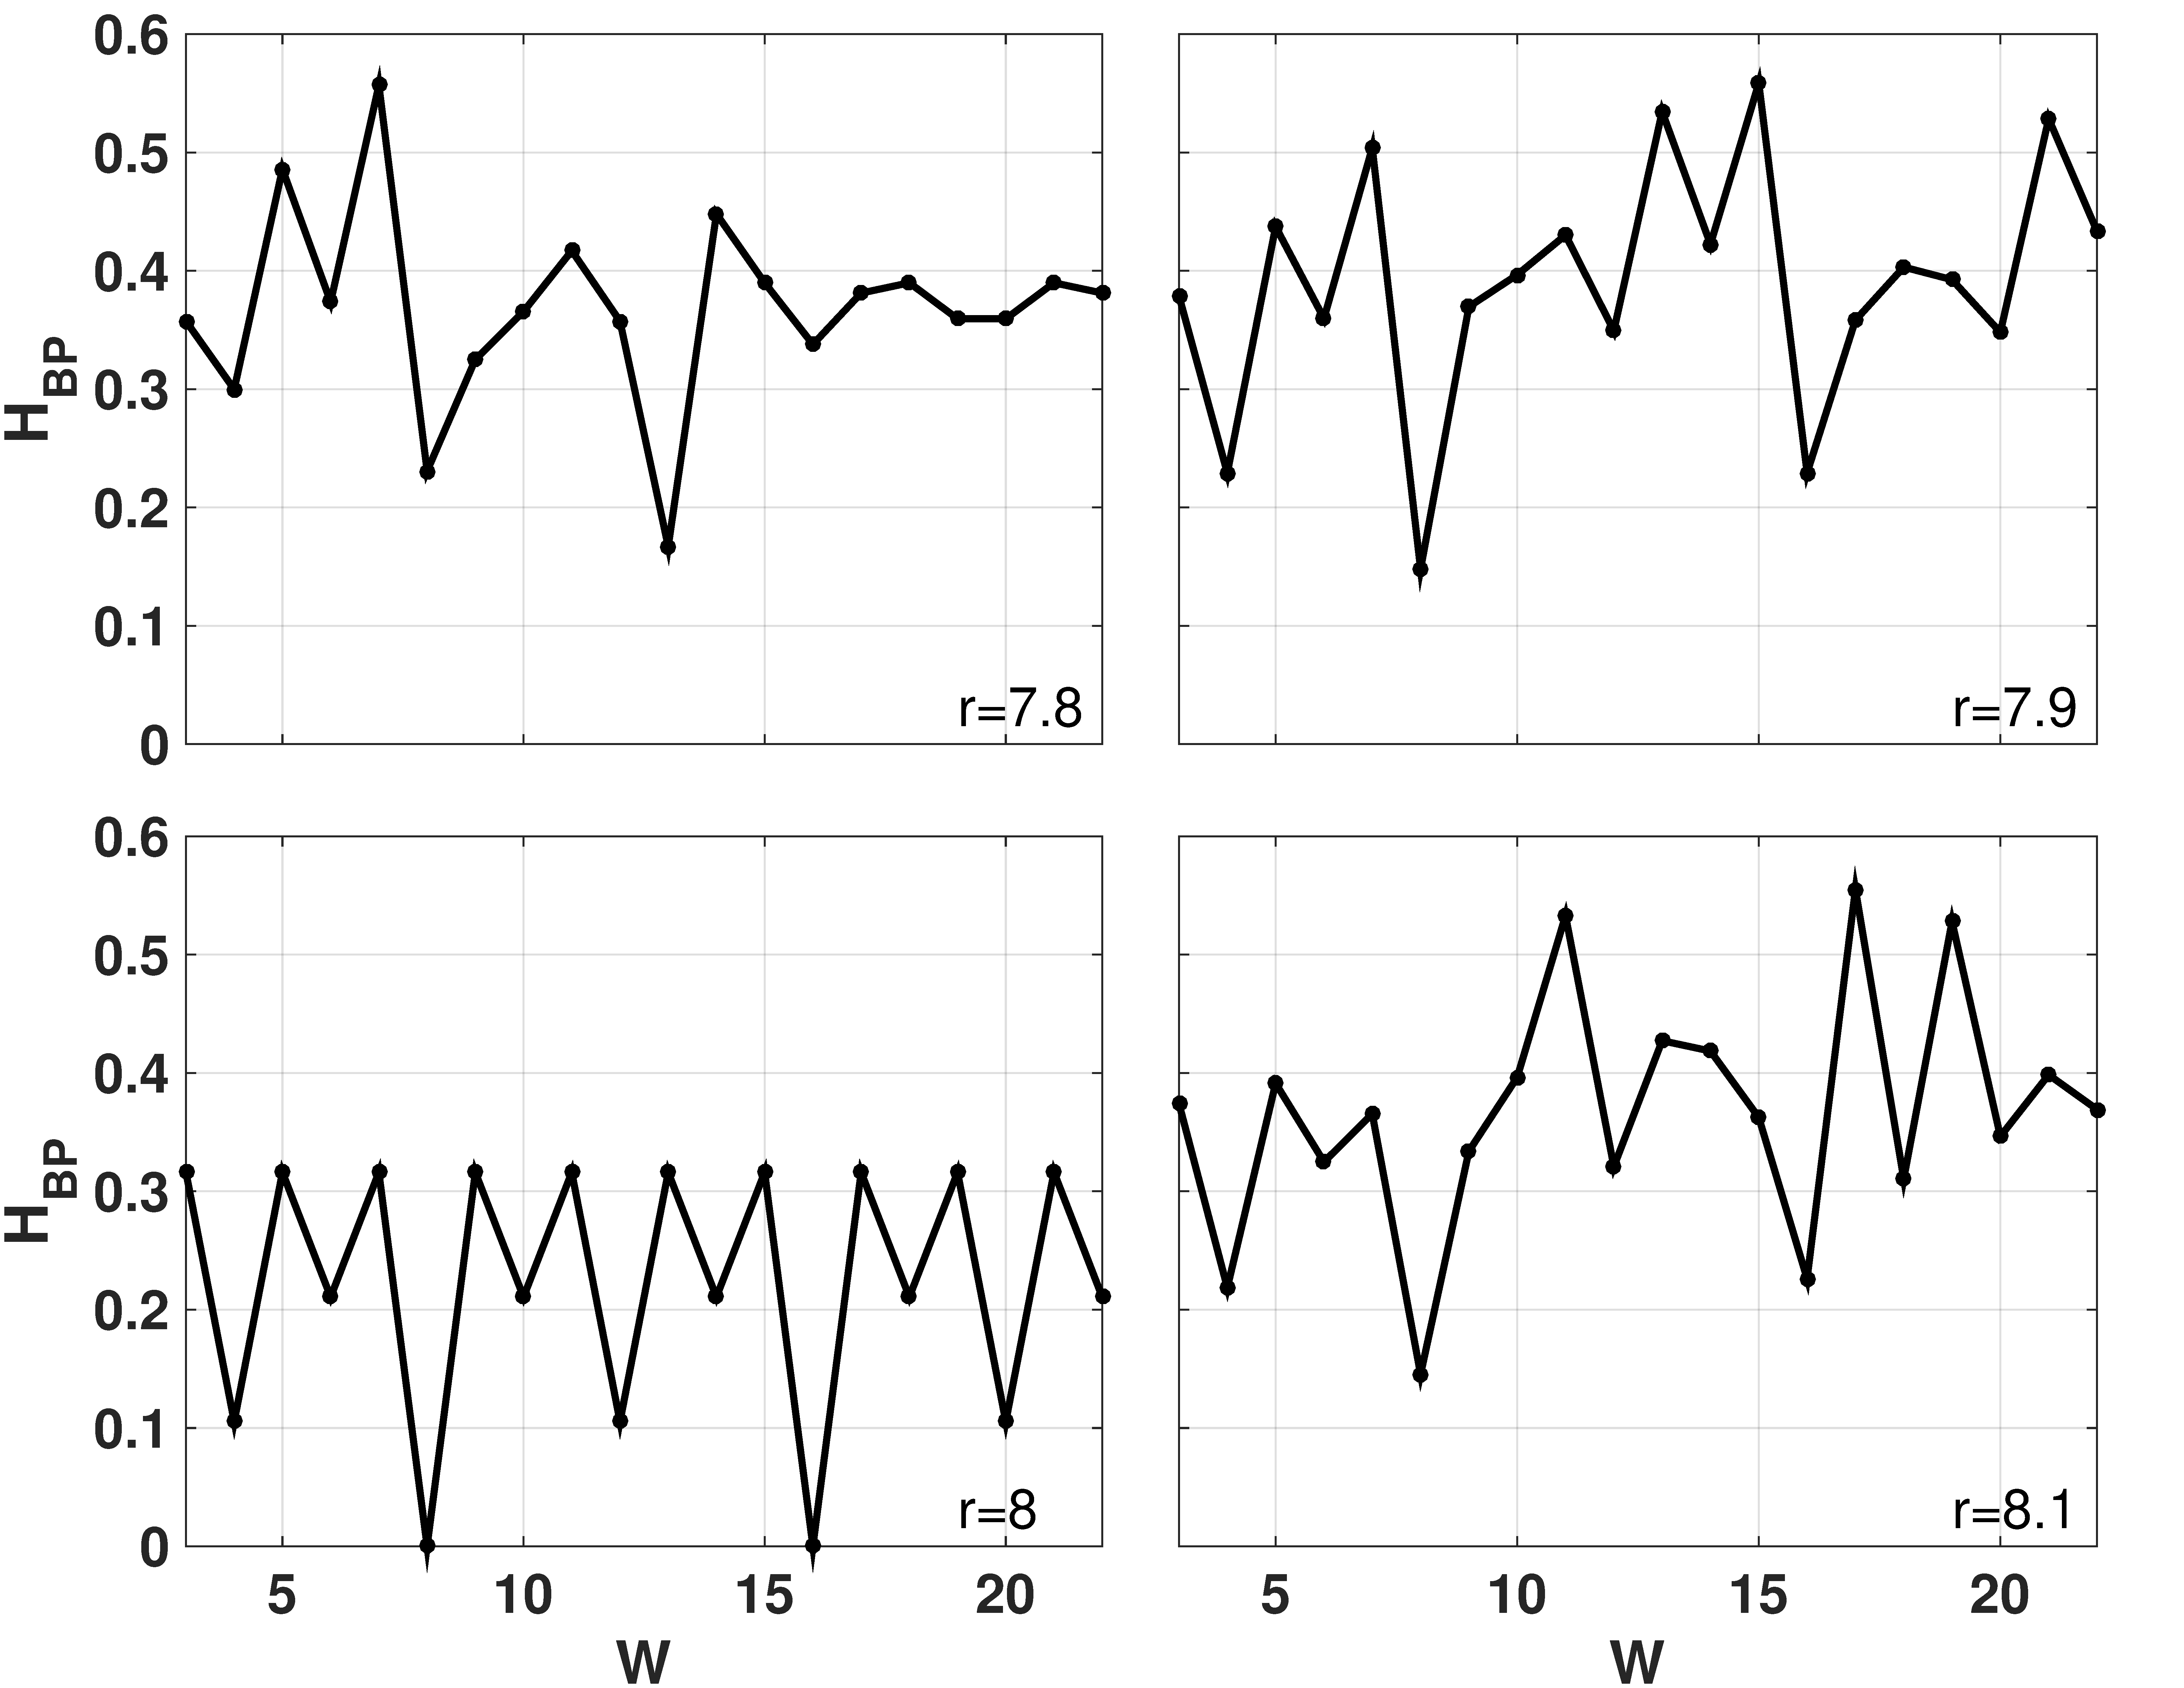
\includegraphics[ width=0.8\textwidth]{HBP_W_rSS}
\caption{$H^{(D)}_{BP}$ as a function of $W$ for a jitter-less \emph{RO} sampled with different values of $r$. Calculations are made without superposition of words}
\label{fig:HBP_W_rSS}
\end{figure}

Our results show that two quantifiers, $h$ and $h^*$, are appropriate to be used as jitter measures because: 
\begin{itemize} 
\item (a) for $\sigma_T=0$ (jitter-less output) they rapidly approach to a constant limiting value as both $D$ and $W$ increase toward $\infty$ and this limiting value is independent of both $D$ and $W$; 
\item (b) they are increasing monotone (and almost proportional) functions of $\sigma_T$. \item (c) From their analysis, it is possible to detect the optimum value of the sampling ratio $r$. Let us show these claims in the following figures that are representative of all our results. 
\end{itemize}
%
Figure \ref{fig:hm_D_SJ} shows the Bandt \& Pompe differential entropy $h^*$, as a function of $D$, with $W$ as a parameter, for a ring without jitter. It can be seen that there is a threshold value $W=4$ over which all the curves collapse into one for every value of $D$. Furthermore, Fig. \ref{fig:hm_D_SJ} also shows that for $D\ge8$ all the curves collapse into one, regardless the value of $W$. In conclusion, if $D\ge 8$ and $W\ge 4$ one obtains a quantifier independent of both $D$ and $W$. The influence of jitter on this quantifier is shown in Figure \ref{fig:hm_D_CJ}, where $h^*$ is plotted as a function of $D$ with $\sigma_T$ as a parameter. The values considered are $\sigma_T=\{0 (no~jitter),$ $0.001,$ $0.002,$ $0.003,$ $0.004,$ $0.005,$ $0.007,$ $0.01,$ $0.02,$ $0.02,$ $0.04,$ $0.05,$ $0.07,$ $0.1\}$. The inset of Fig. \ref{fig:hm_D_CJ} shows $h^*$ as a function of $\sigma_T$ for $D=8$. This inset shows that this quantifier is an increasing monotone function of $\sigma_T$. Finally Fig. \ref{fig:hm_r_CJ} shows $h^*$ as a function of the sampling ratio $r$. 
In this figure, it is shown that there is a minimum for the right $r$ (in this case $r=8$). Furthermore sensitivity of $h^*$ as a function of jitter is maximum for this same ideal value of $r$.

\begin{figure}
\center
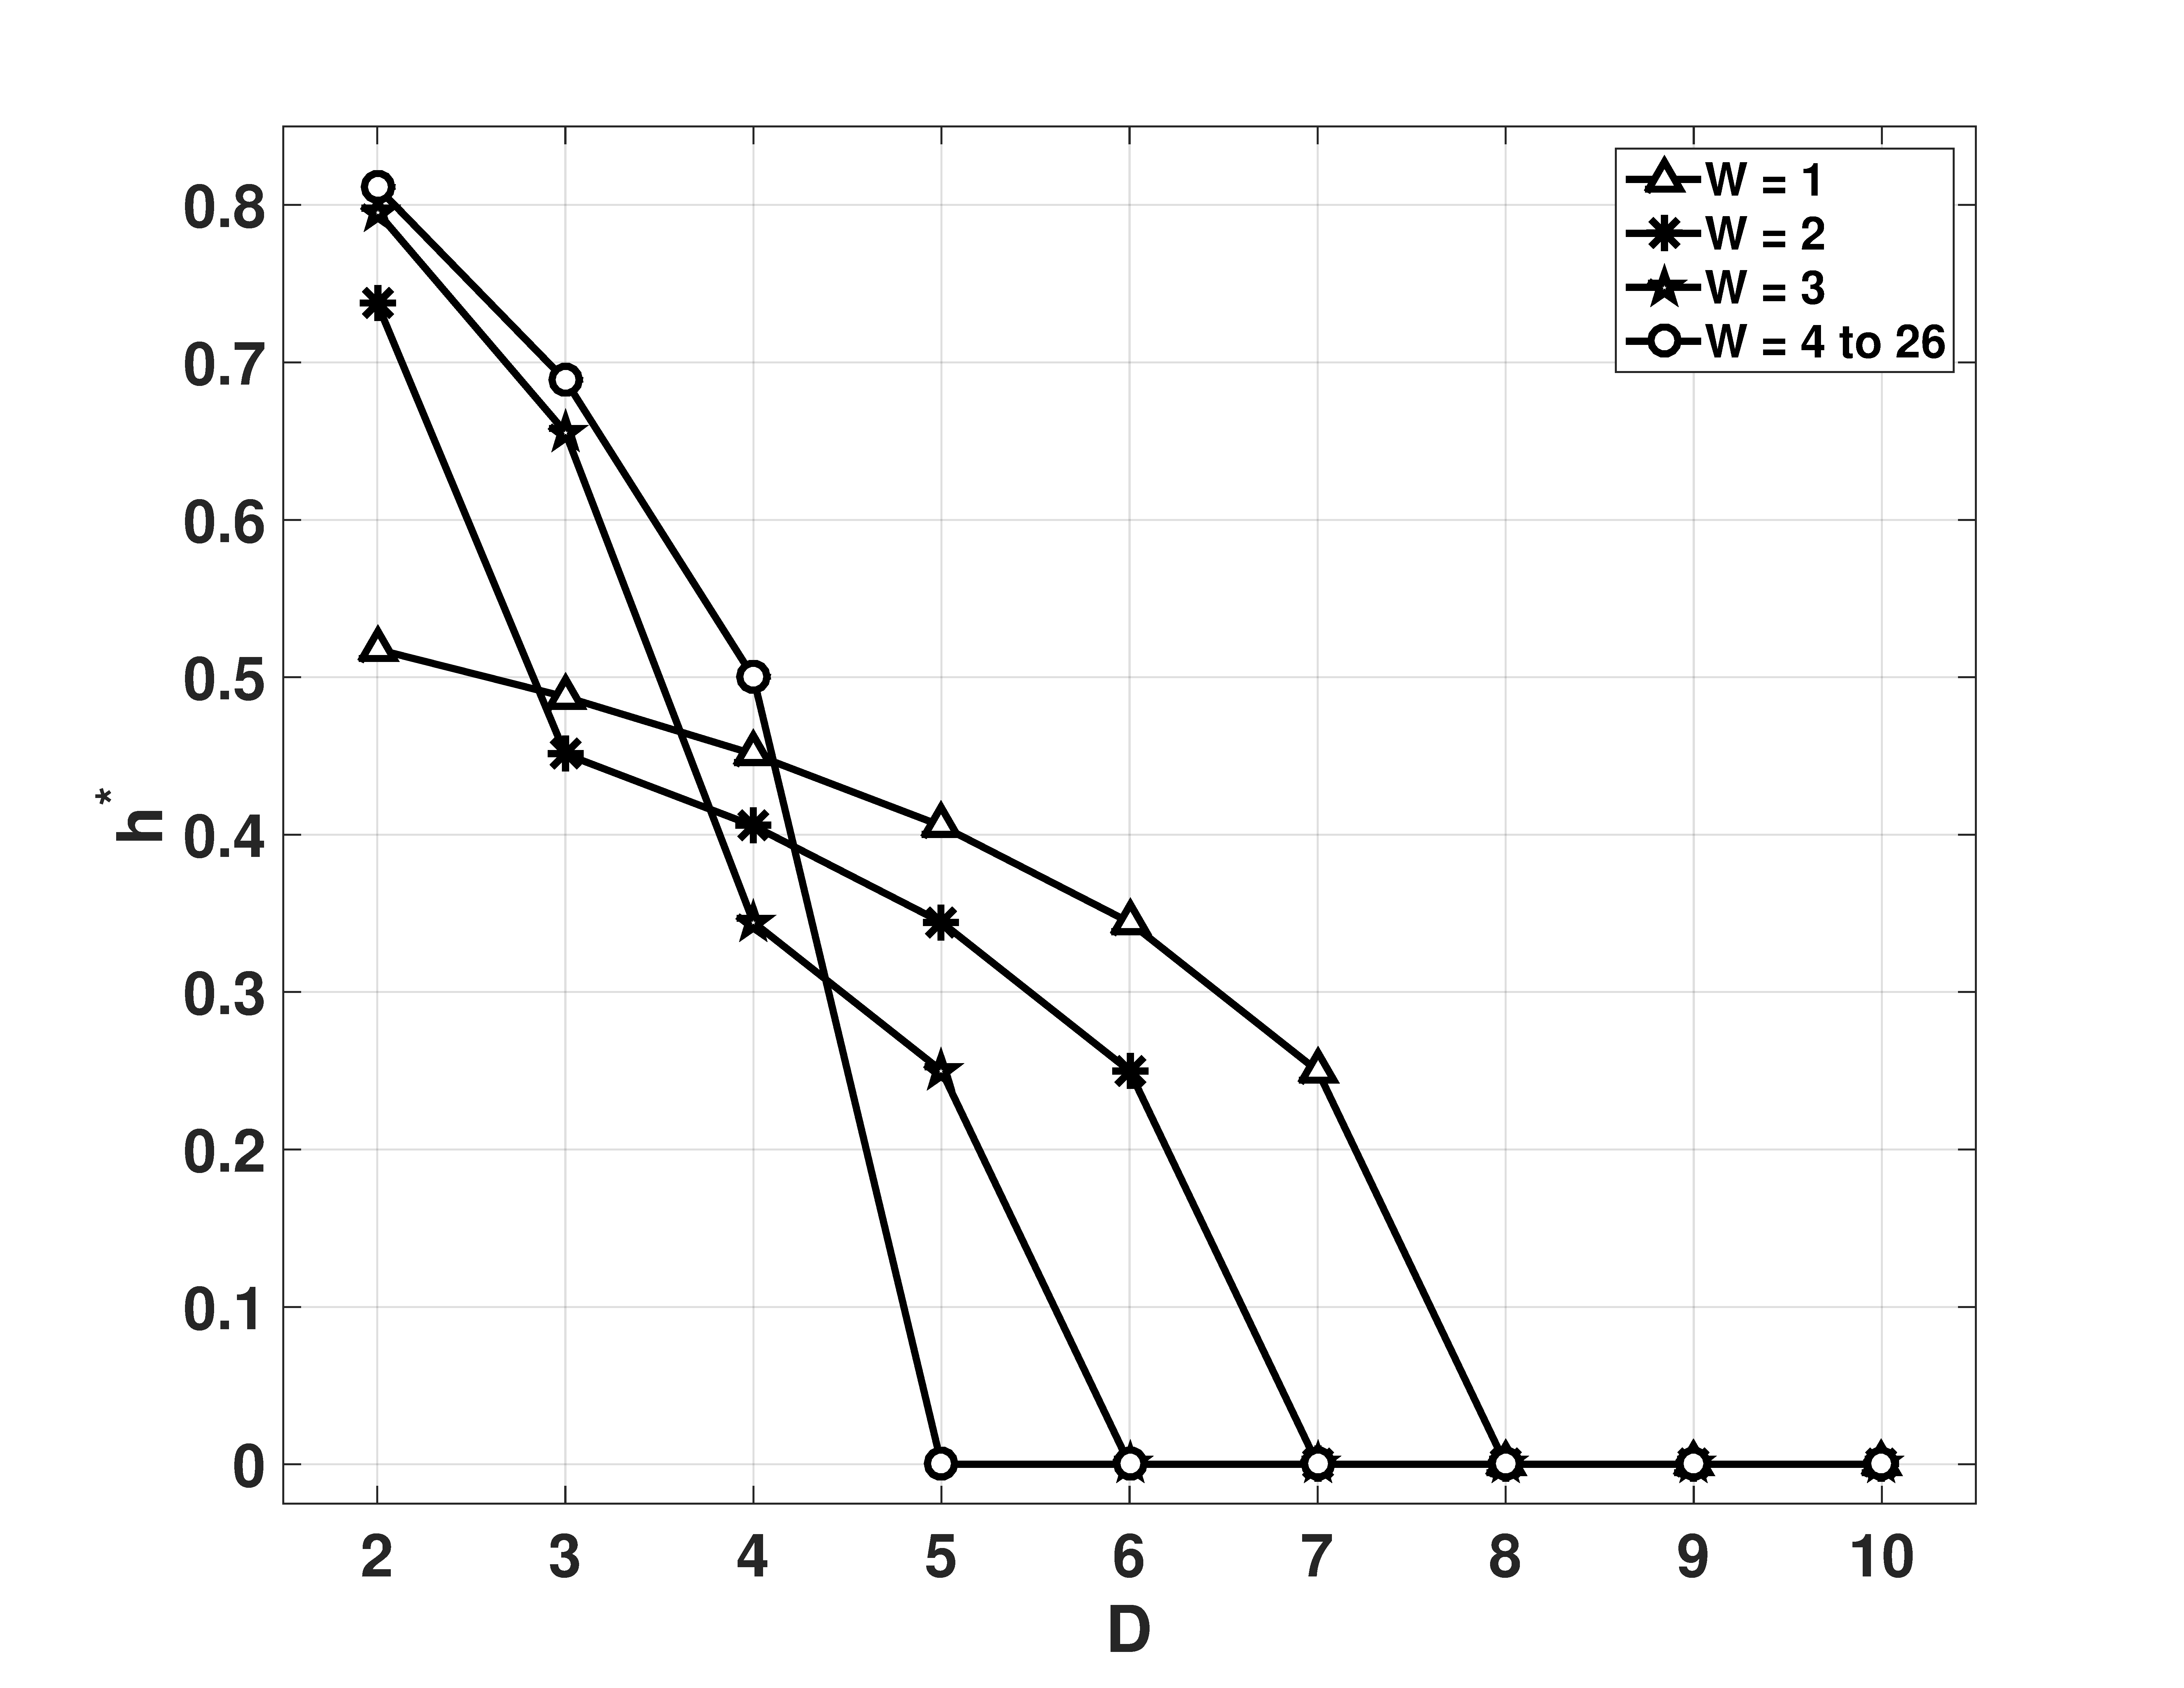
\includegraphics[ width=0.8\textwidth]{hm_D_SJ}
\caption{$h^*$ as a function of $D$ for a jitter-less \emph{RO} sampled with $r=8$.}
\label{fig:hm_D_SJ}
\end{figure}

\begin{figure}
\center
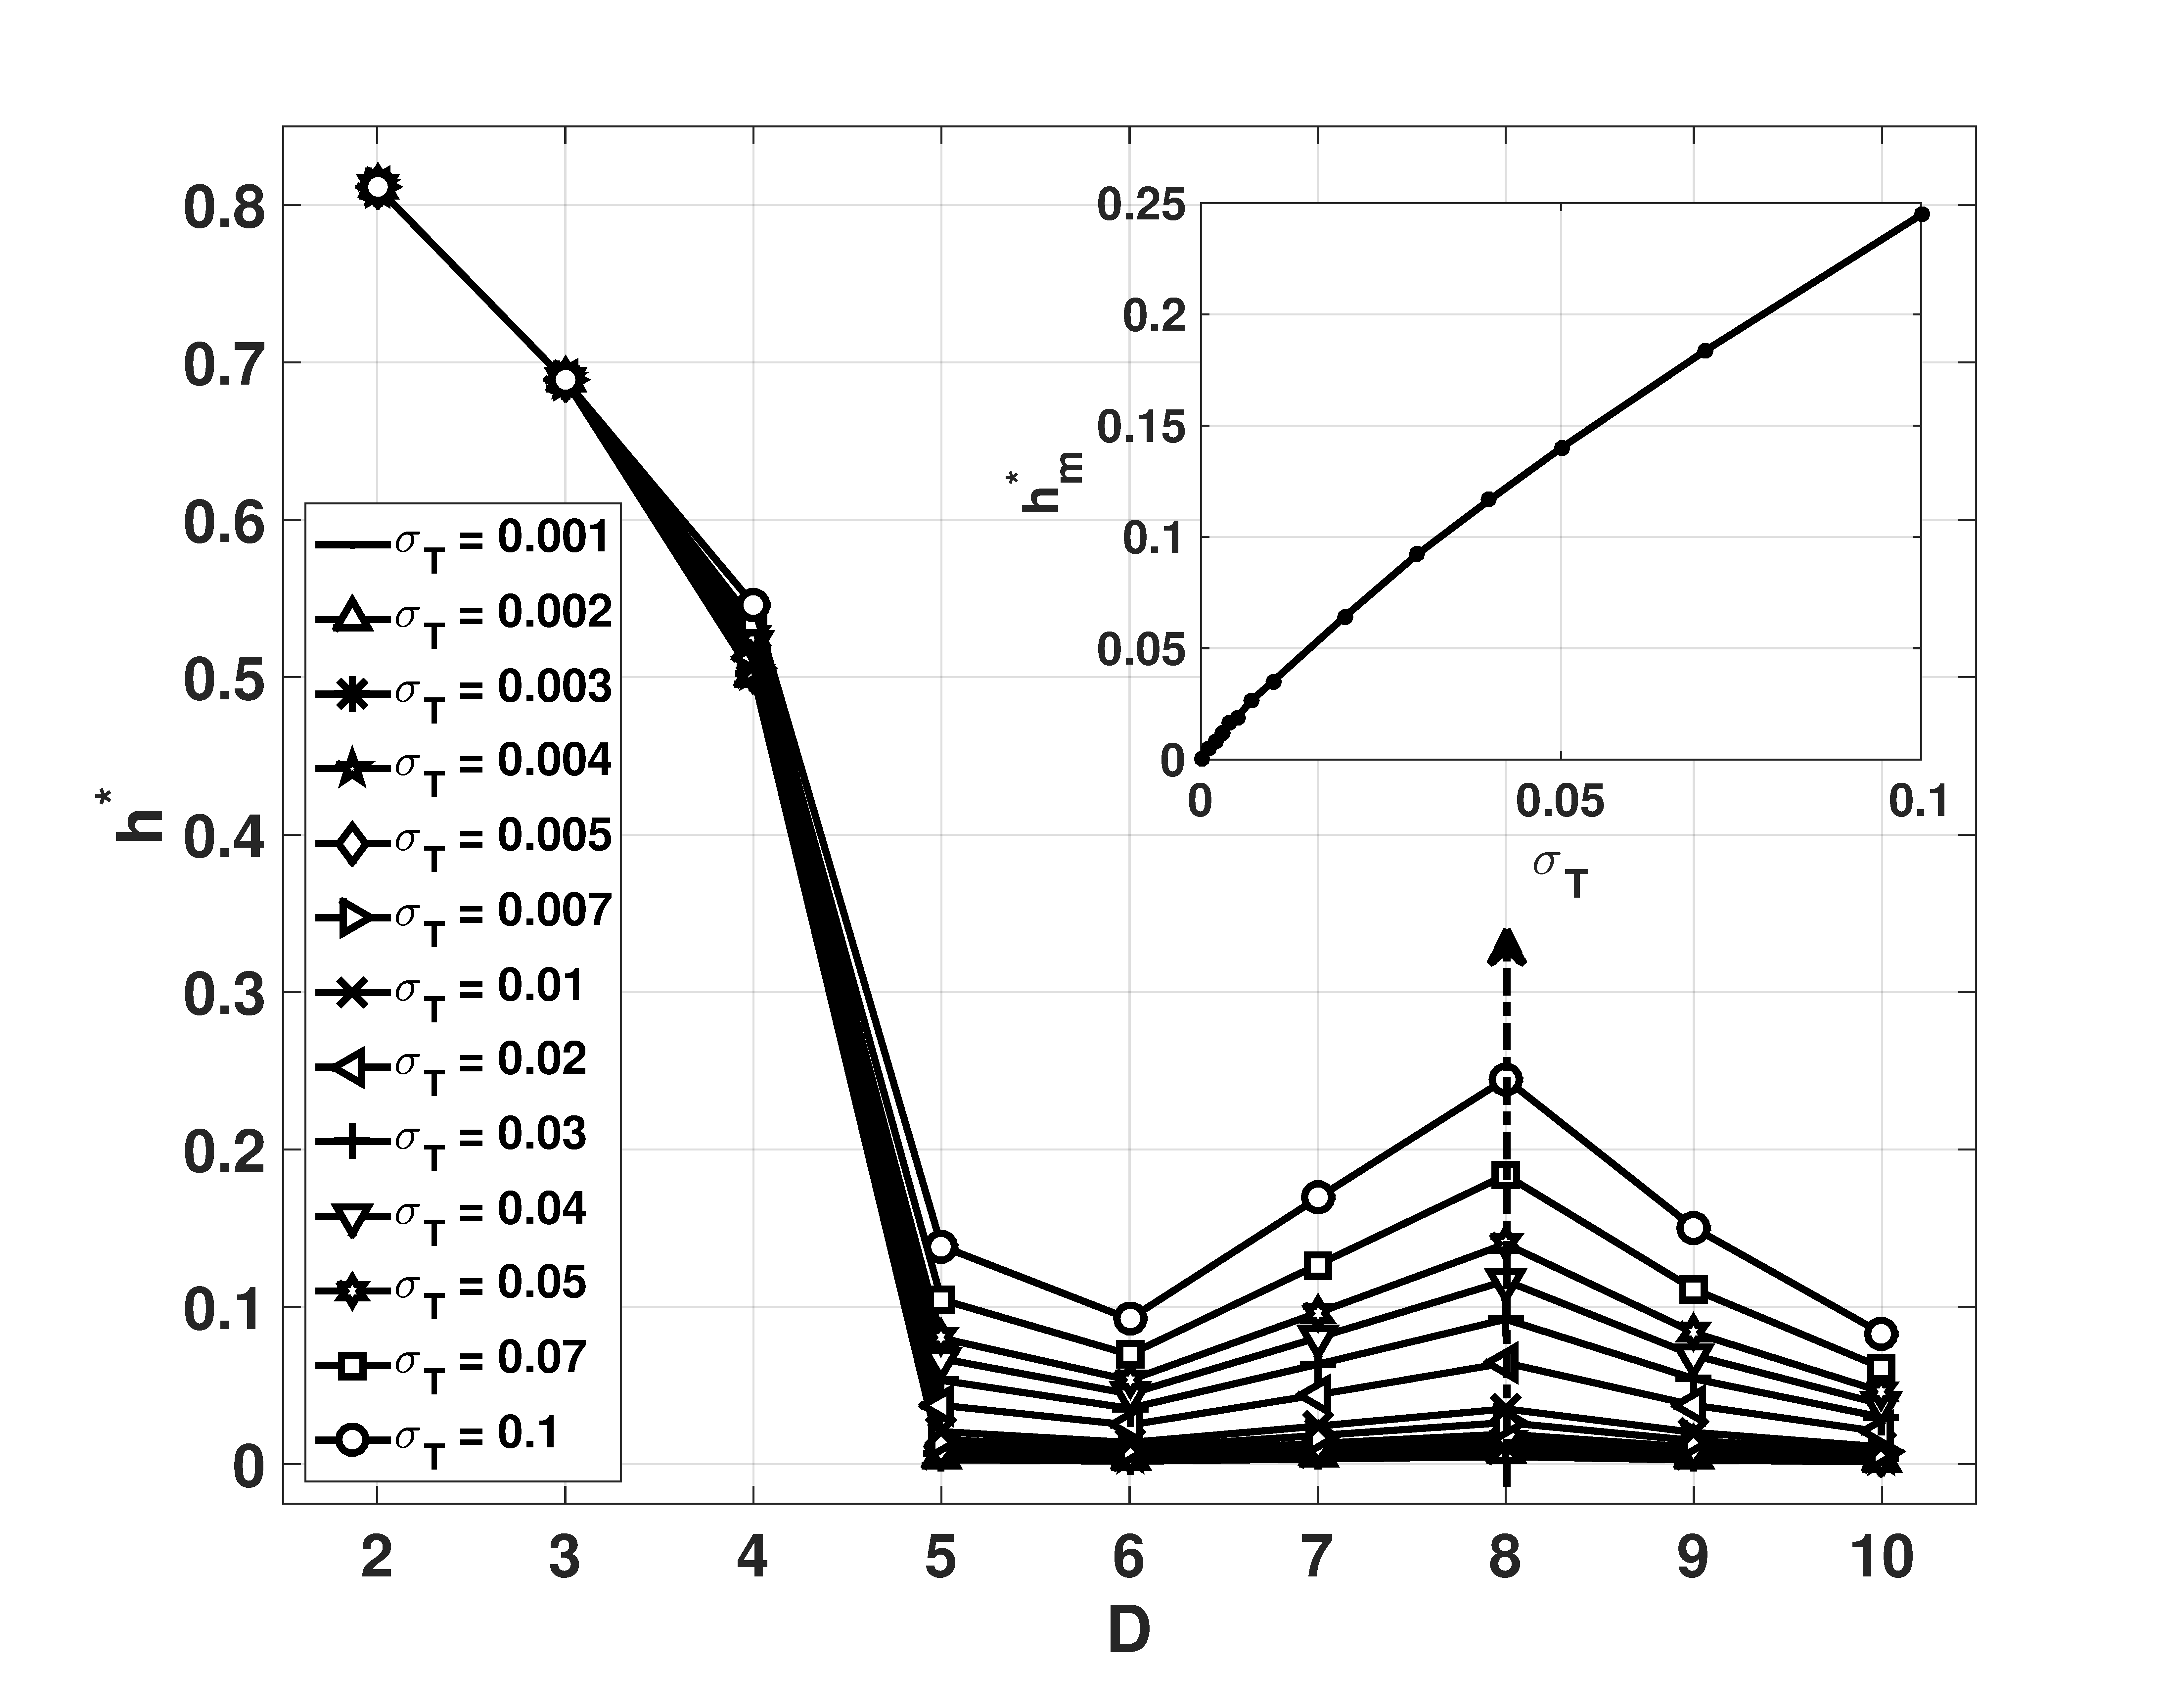
\includegraphics[width=0.8\textwidth]{hm_D_CJ}
\caption{$h^*$ as a function of $D$ for a \emph{RO} sampled with $r=8$ for a world length $W=6$ for jitter with several variances. The inset shows $h^*$ as a function of $\sigma_T$ for $r=8$, $W=6$ and $D=8$.}
\label{fig:hm_D_CJ}
\end{figure}

\begin{figure}
\center
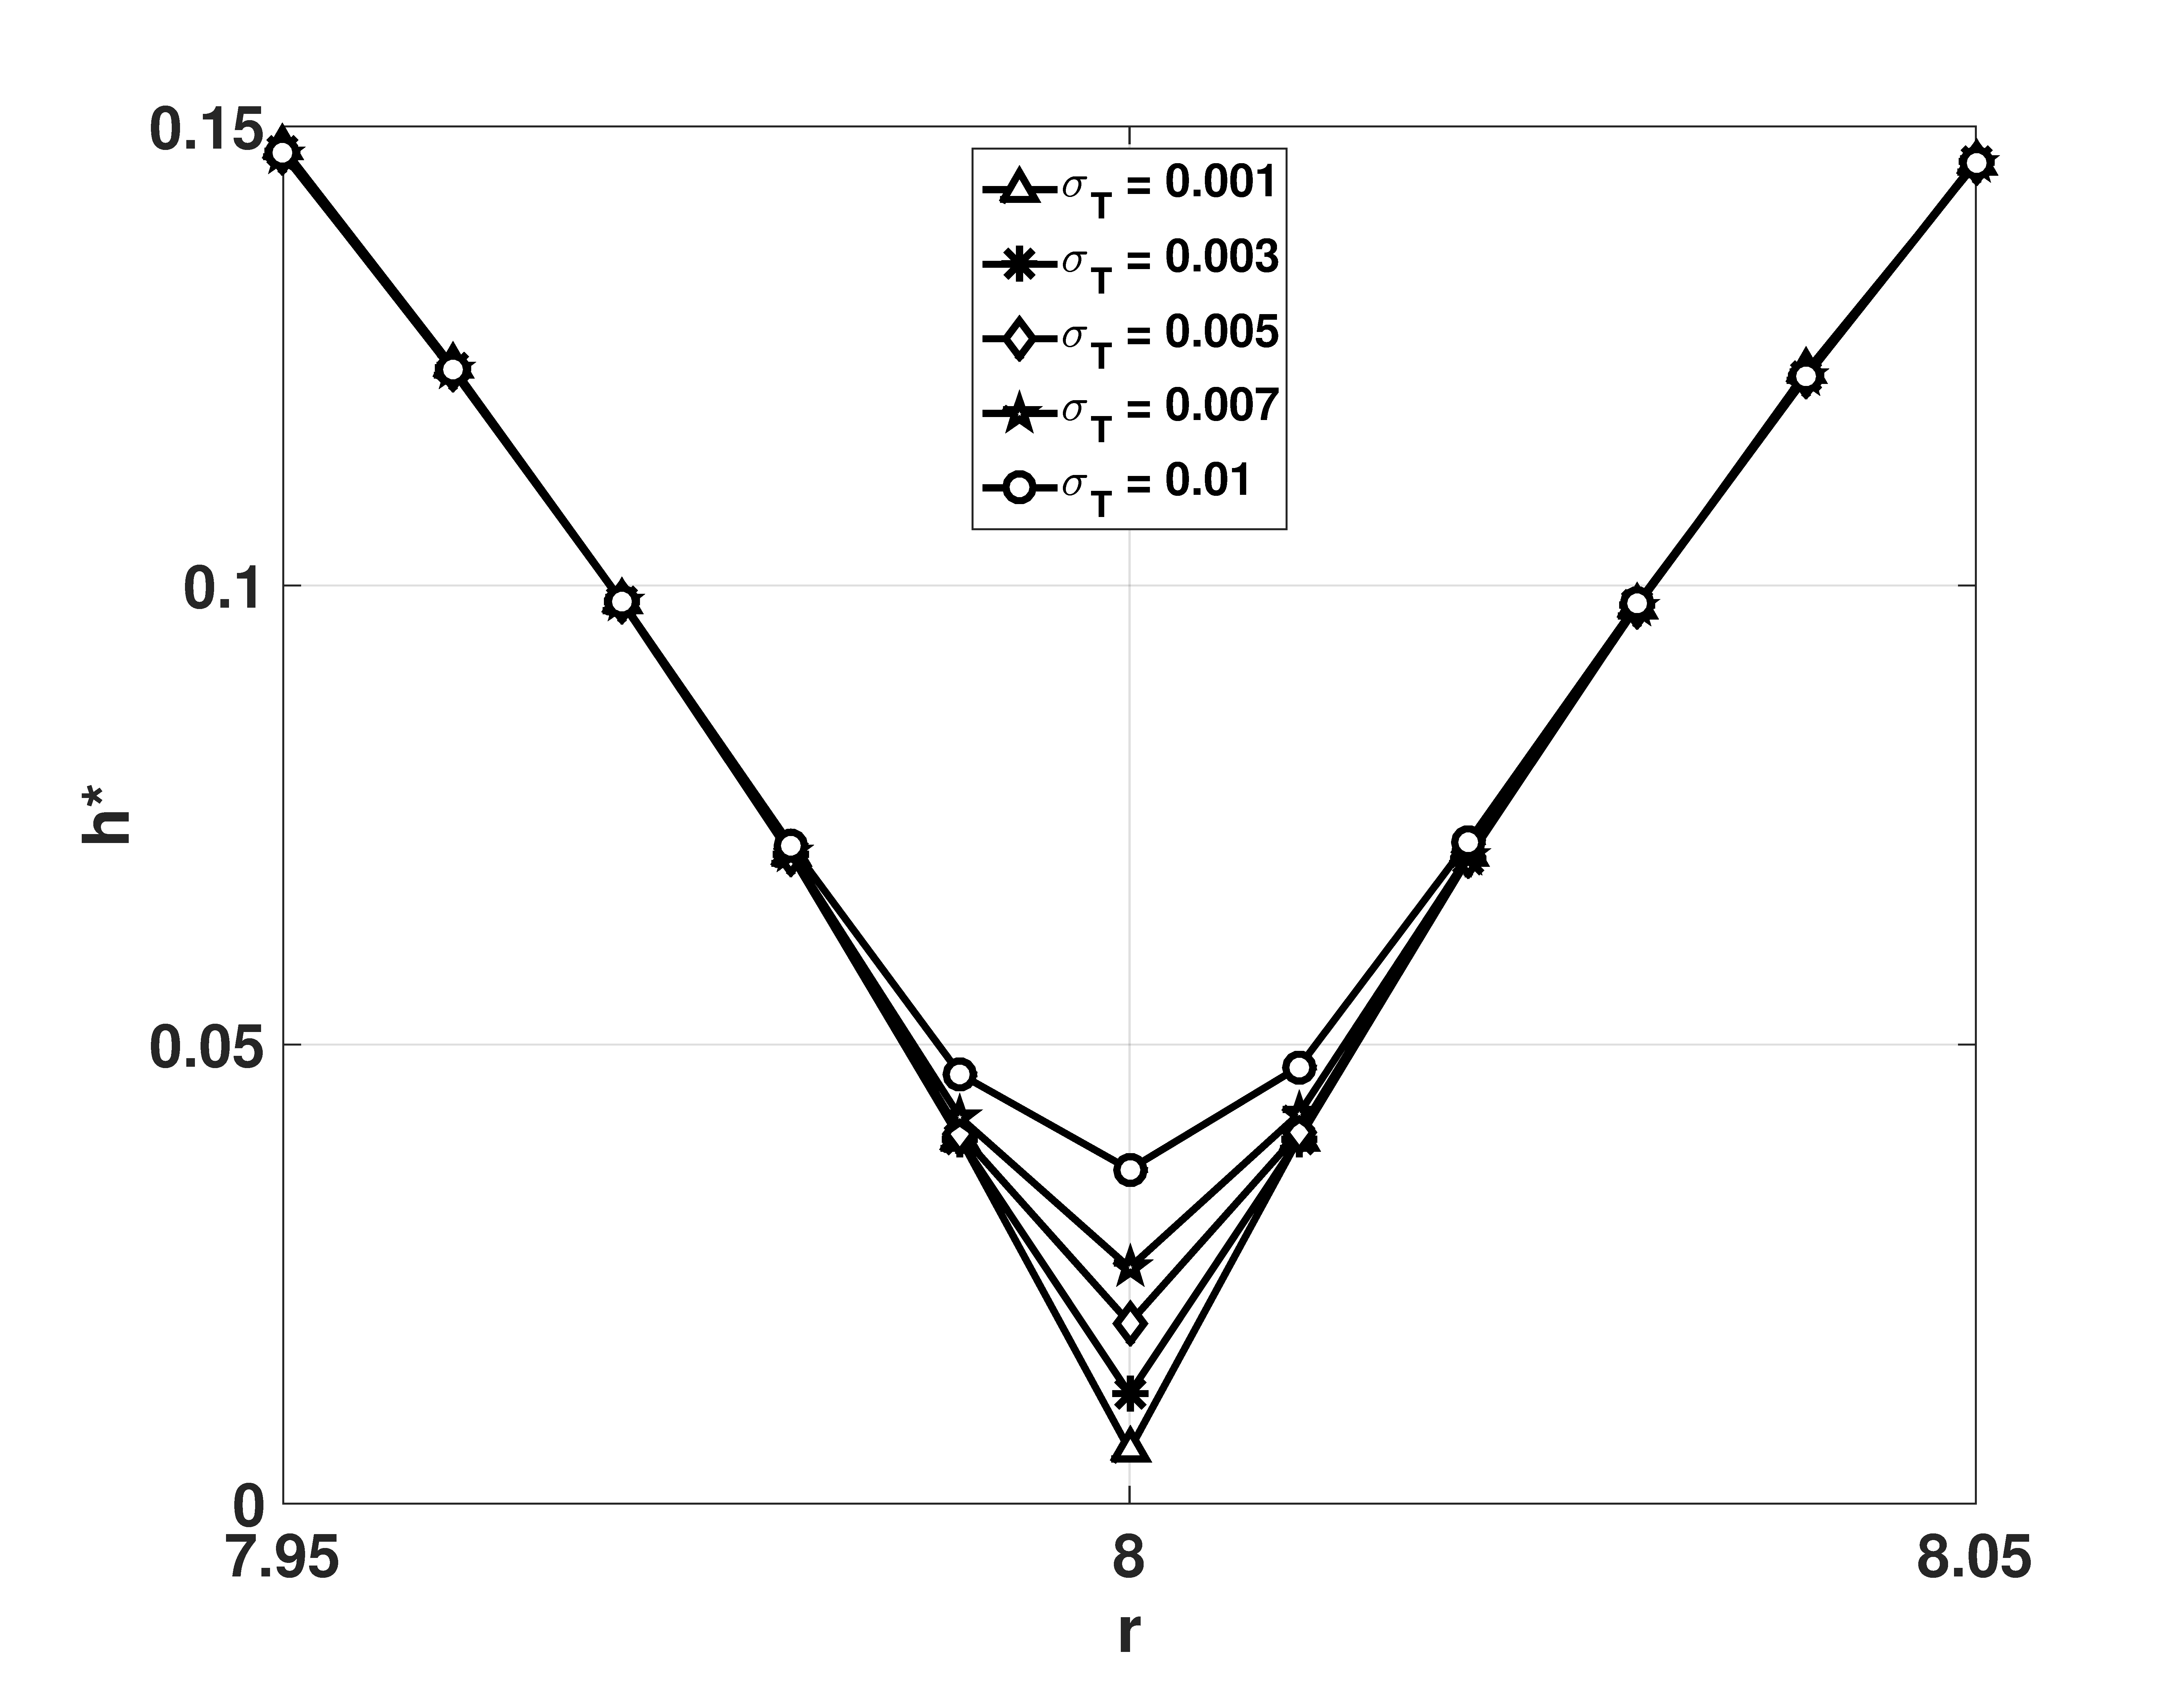
\includegraphics[ width=0.8\textwidth]{hm_r_CJ}
\caption{$h^*$ as a function of $r$ for $r\in[7.95,8.05]$, with several $\sigma_T$, $W=6$ and $D=8$. The curve has a minimum at the correct value $r=8$.}
\label{fig:hm_r_CJ}
\end{figure}

Let us now analyze the second quantifier, $h$. This quantifier only depends on $W$ because $D$ is not used to define the \emph{PDF} assigned to the data series. Fig. \ref{fig:h_W_SJ} shows jitter-less case, $h$ is almost independent of $W$ for $W\ge4$. In this paper, we adopted $W=6$. Figure \ref{fig:h_W_CJ} shows the influence of jitter over this quantifier. It is clear from the inset in this figure that, for the selected value $W=6$, $h$ is an increasing monotone function of jitter variance $\sigma_T$.

Fig. \ref{fig:h_r_CJ} shows that $h$ has a minimum when the value of $r$ takes its optimum value ($r=8$). Note that this minimum is robust also in the presence of jitter.

\begin{figure}
\center
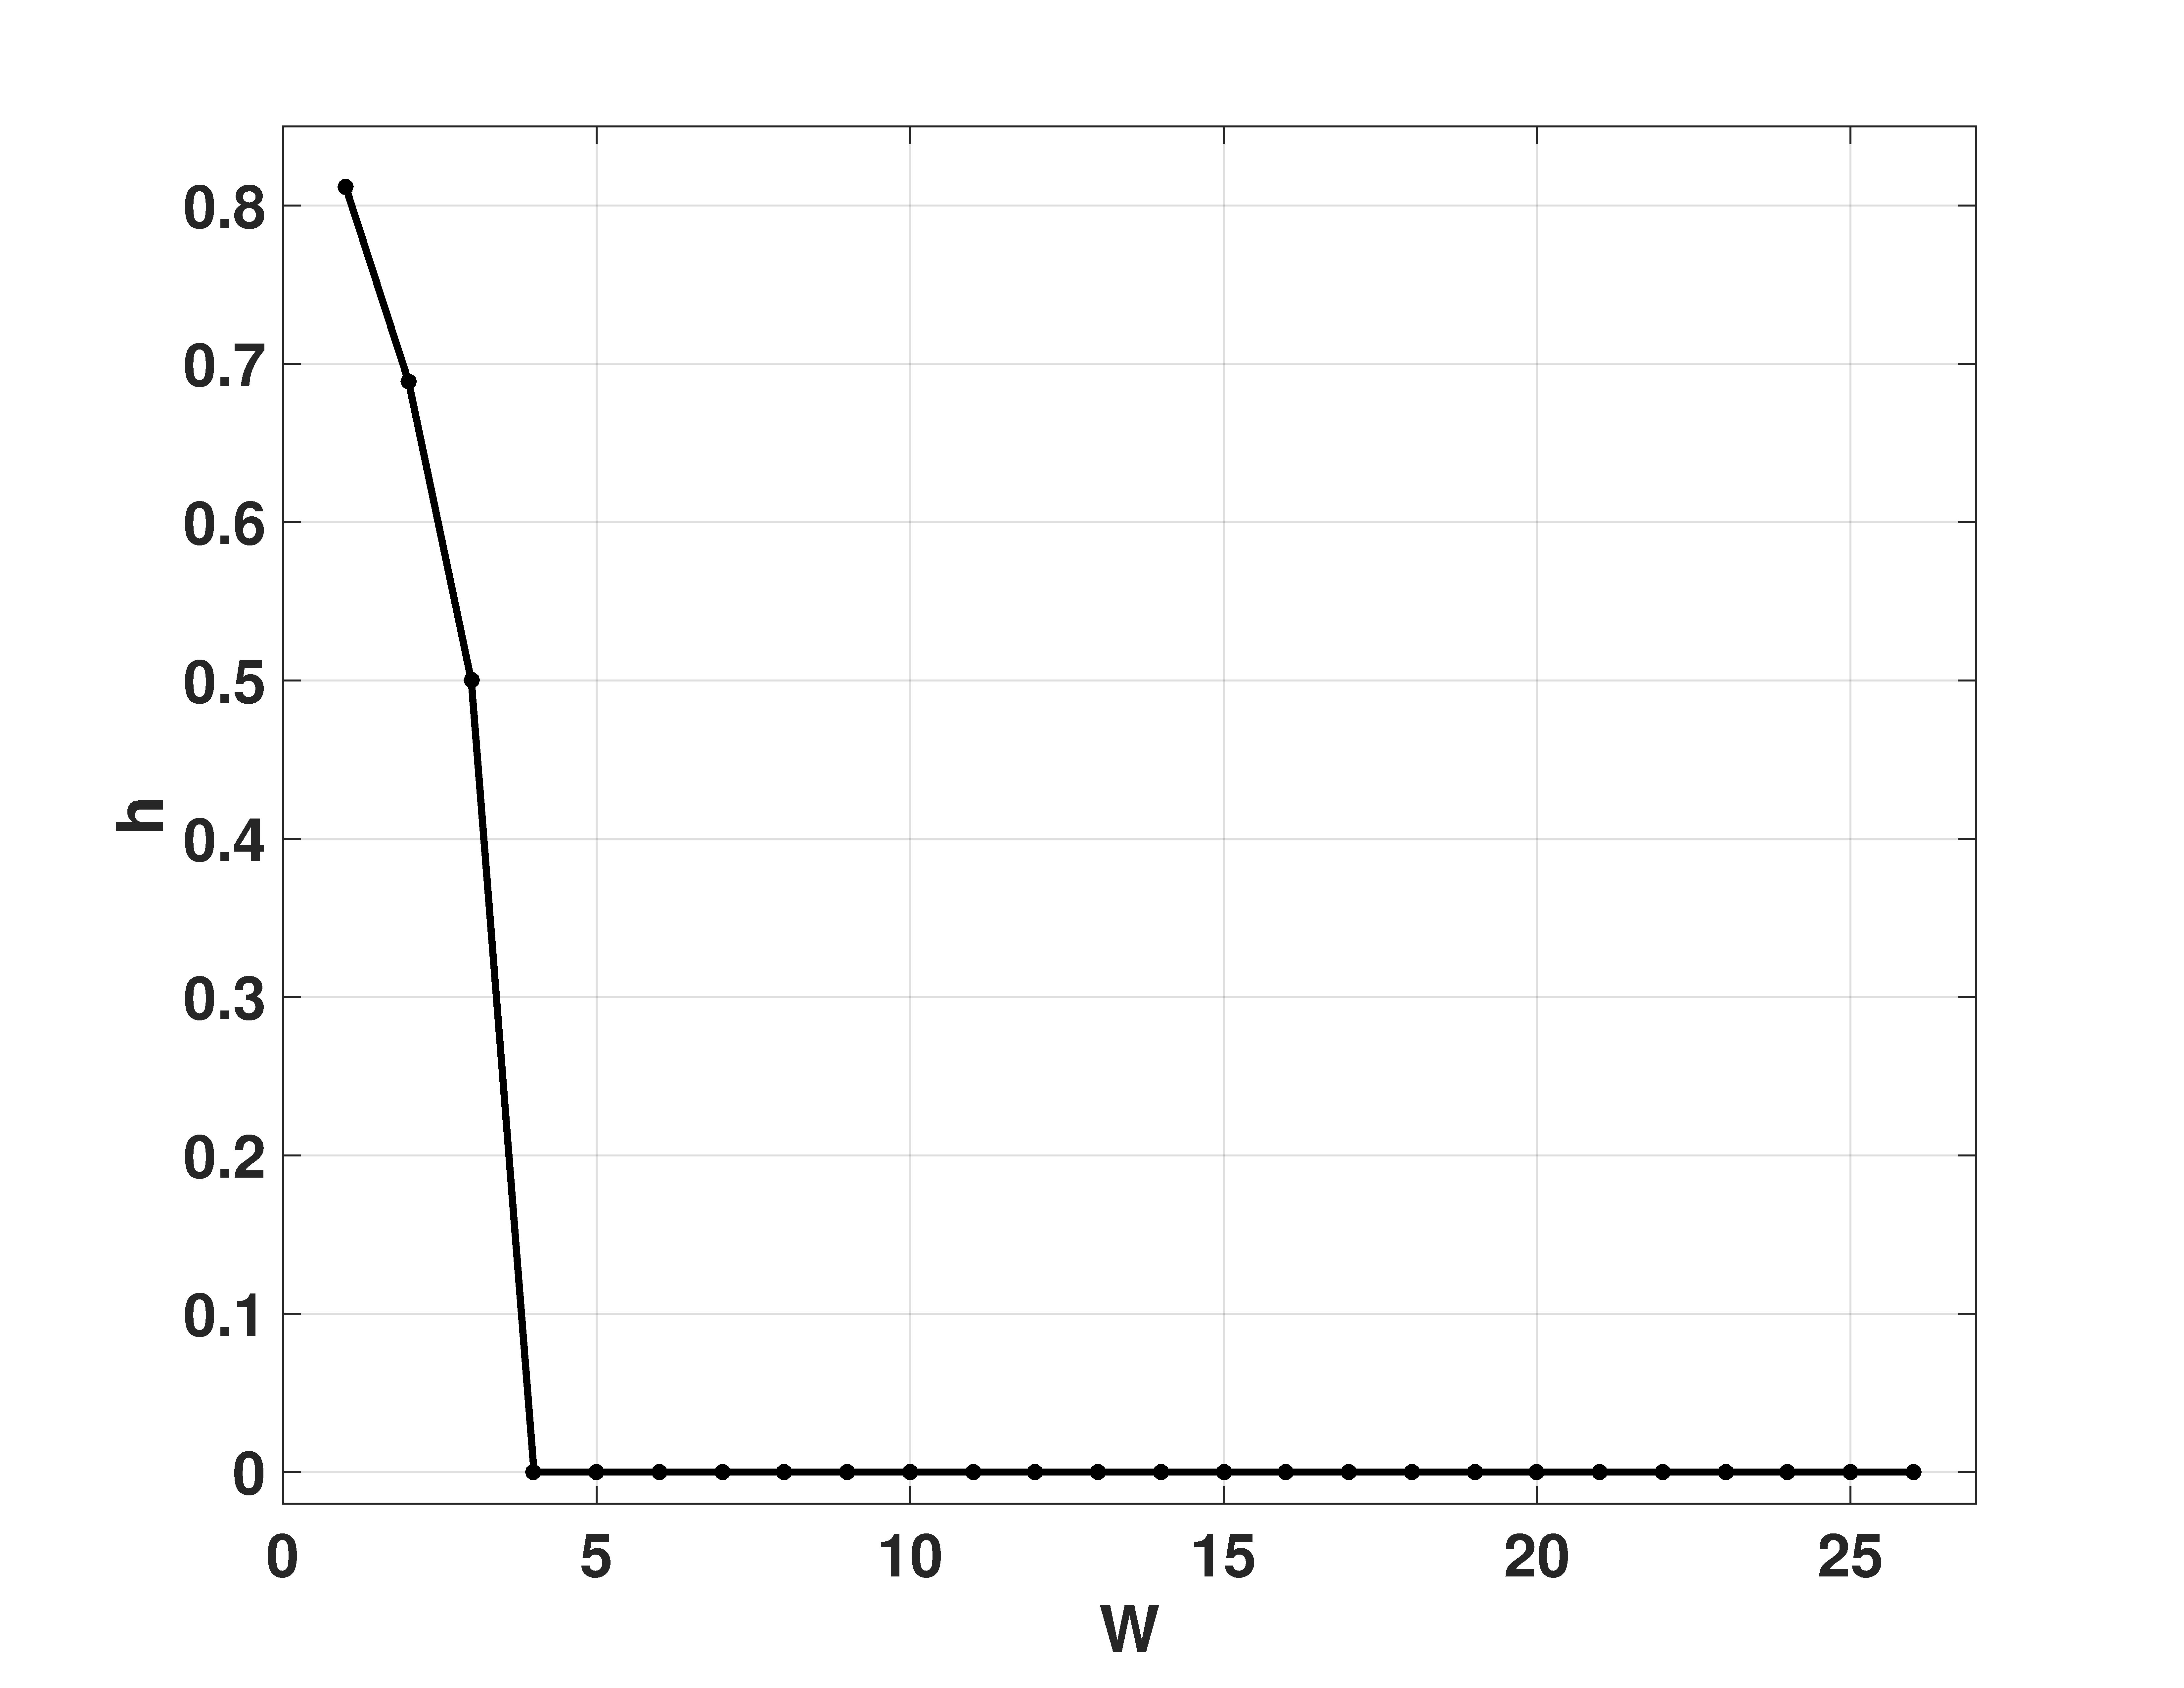
\includegraphics[width=0.8\textwidth]{h_W_SJ}
\caption{$h$ as a function of $W$ for a jitter-less \emph{RO} sampled with $r=8$.}
\label{fig:h_W_SJ}
\end{figure}

\begin{figure}
\center
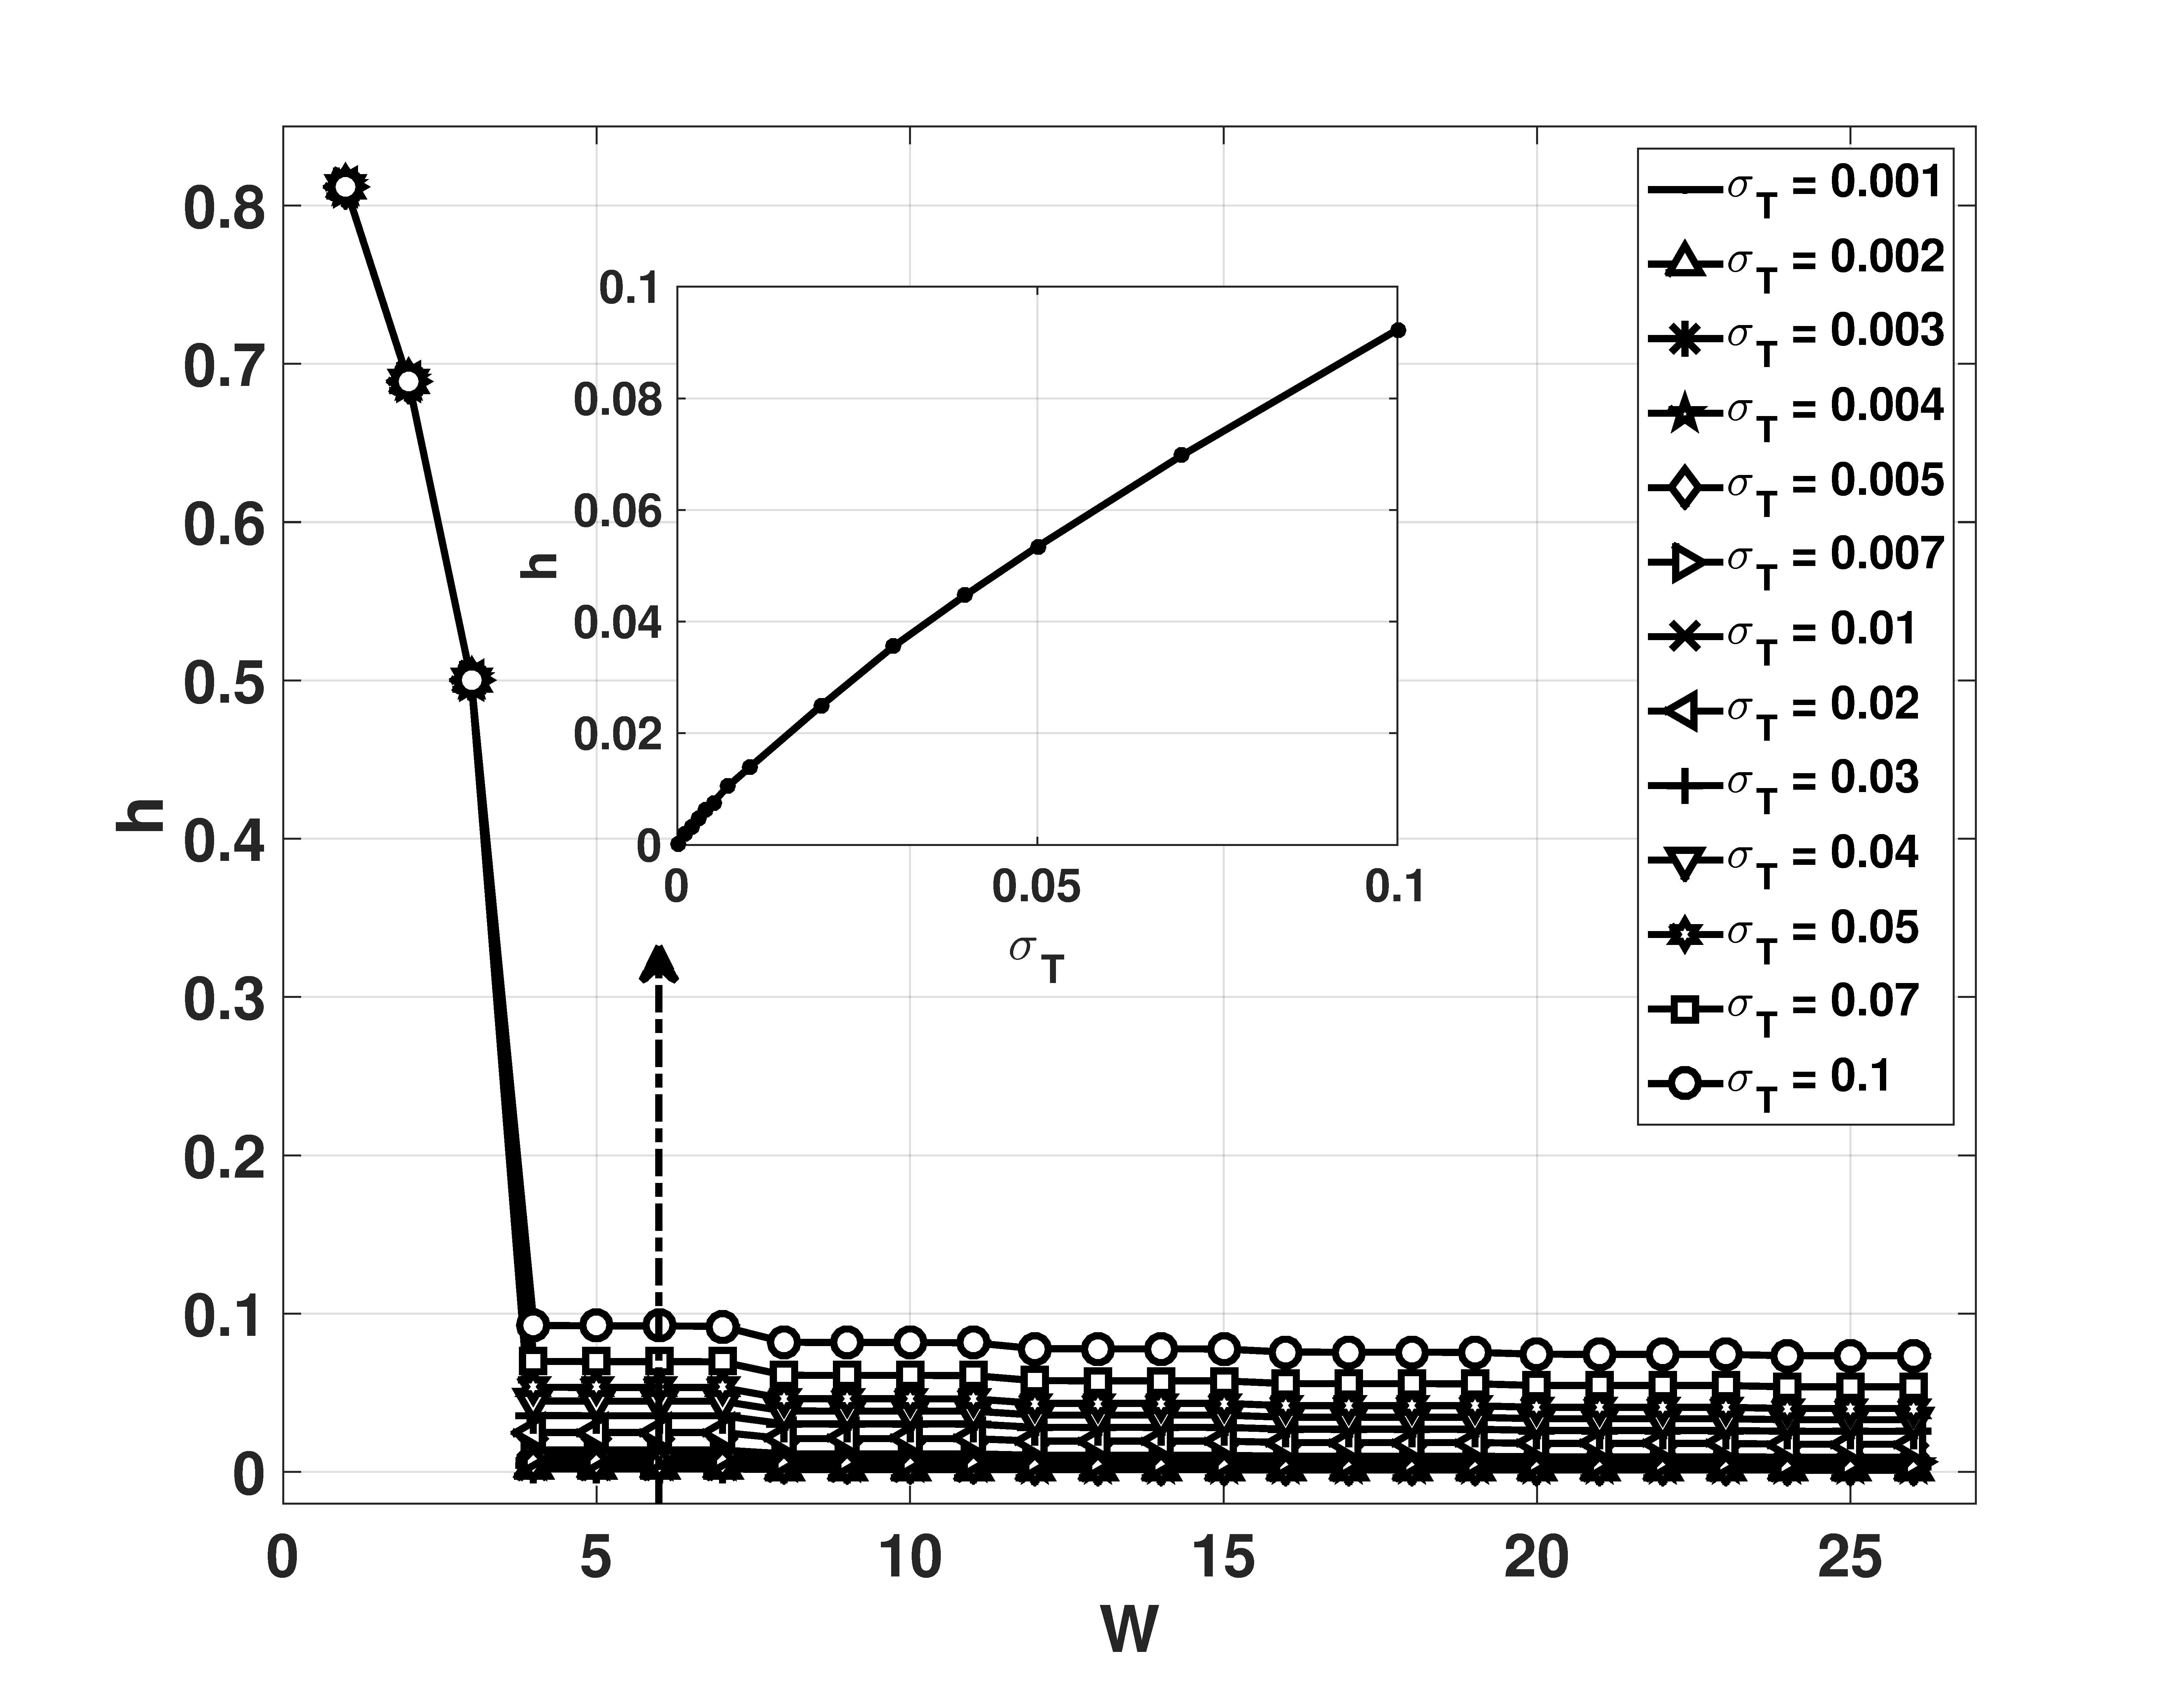
\includegraphics[ width=0.8\textwidth]{h_W_CJ}
\caption{$h$ as a function of $W$ for a \emph{RO} sampled with $r=8$, for jitter with several variances. The inset shows $h$ as a function of $\sigma_T$ for $r=8$ and $W=6$.}
\label{fig:h_W_CJ}
\end{figure}

\begin{figure}
\center
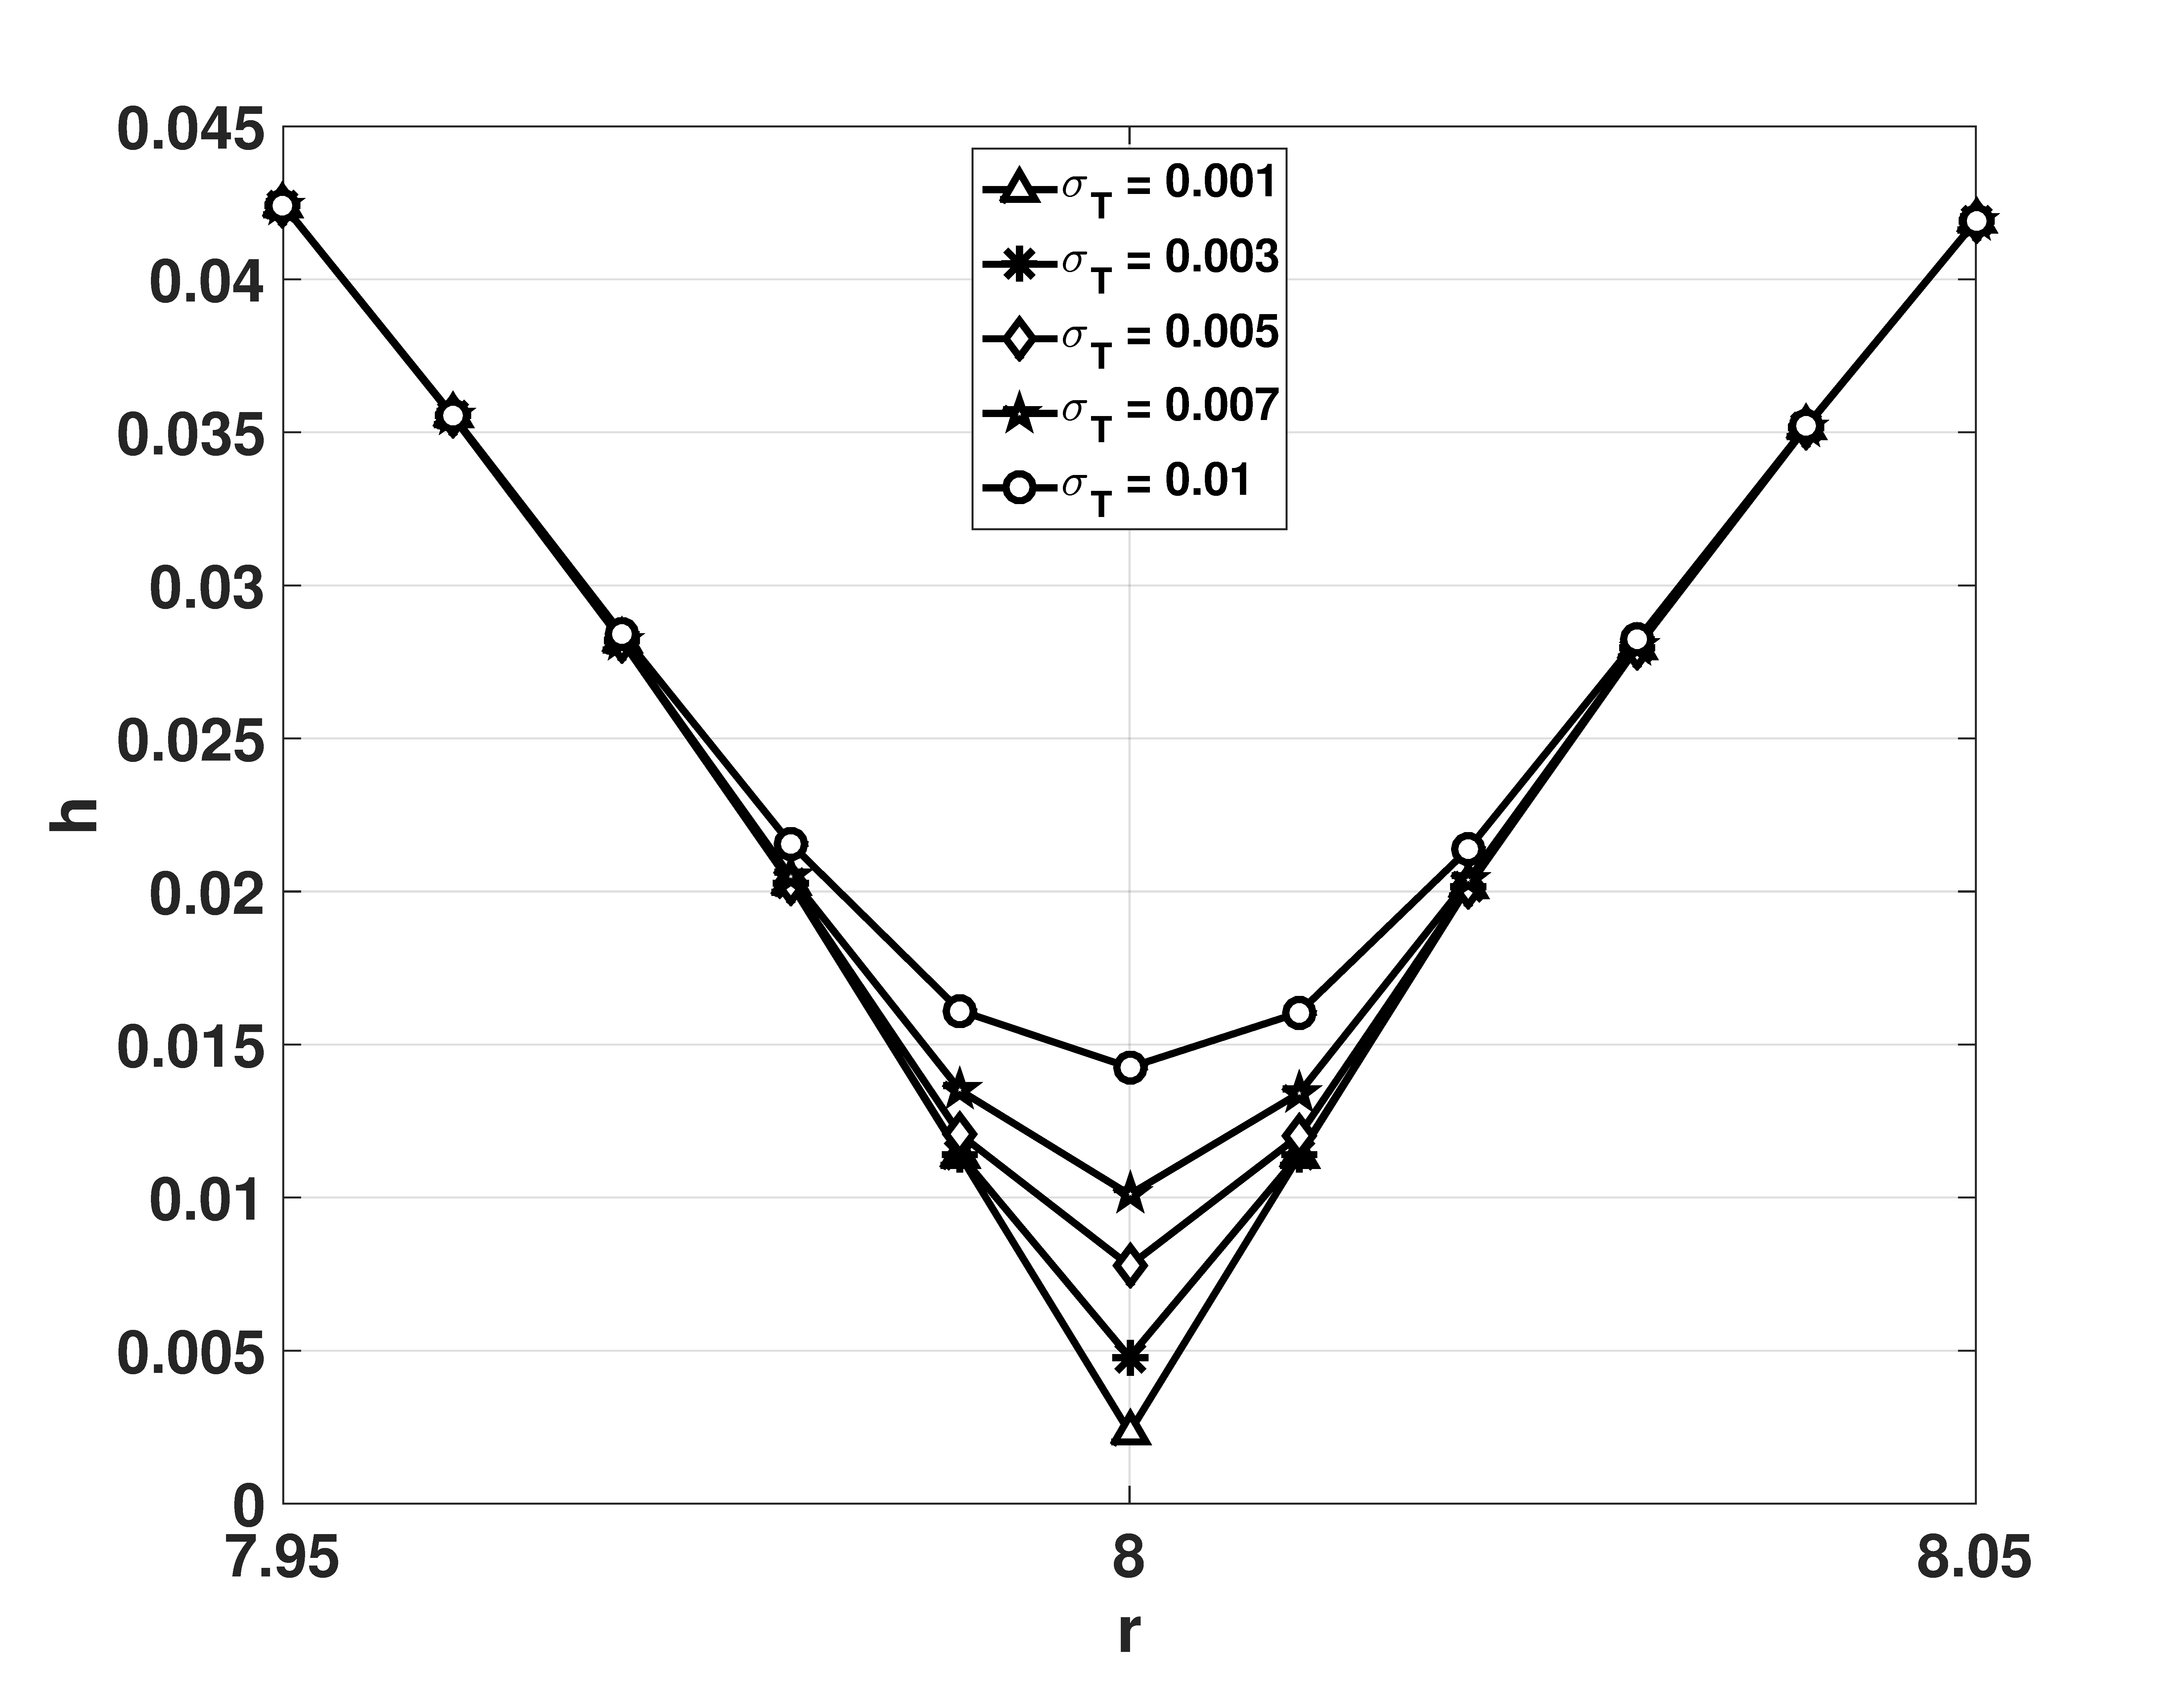
\includegraphics[ width=0.8\textwidth]{h_r_CJ}
\caption{$h$ as a function of $r$ for $r\in[7.95,8.05]$, with several $\sigma_T$ and $W=6$ . The curve has a minimum at the optimum value $r=8$.}
\label{fig:h_r_CJ}
\end{figure}

Further analysis must be done to assure that the selected values $W=6$ and $D=8$ produce symbolic files with a good statistics. For a given alphabet $\mathcal{A}$ with $m$ elements, and a given symbolic file of length $n$, the quality parameter $\alpha=n/m$, see \ref{sec:quanti}. Quality is better as $\alpha$ increases and a minimum value $\alpha=10$ was accepted. According to section \ref{sec:quanti} the selected values $W=6$ and $D=8$ provide $\alpha_h\simeq10^5$, $\alpha_{h^*}\simeq175$ with superposition and $29$ without superposition. All cases give $\alpha>10$ as required.

A comparison between both quantifiers is shown in Figure \ref{fig:hm_h_CJ}. Markers correspond to variances $\sigma_T=\{0,$ $0.001,$ $0.002,$ $0.003,$ $0.004,$ $0.005,$ $0.007,$ $0.01,$ $0.02,$ $0.03,$ $0.04,$ $0.05,$ $0.07,$ $0.1\}$.
Note that the slope of any of these curves is $dh^*/dh$ and it is equal to the quotient between slopes of curves in the insets of Figs. \ref{fig:hm_D_CJ}, and \ref{fig:h_W_CJ}. If $dh^*/dh~>1$, $h^*$ is more sensitive than $h$ to measure jitter. The slope slightly increases from $\sim2.47$ for $W=5$ to $\sim5.54$ for $W=19$ showing that $h^*$ becomes more sensitive as $W$ increases.

\begin{figure}
\center
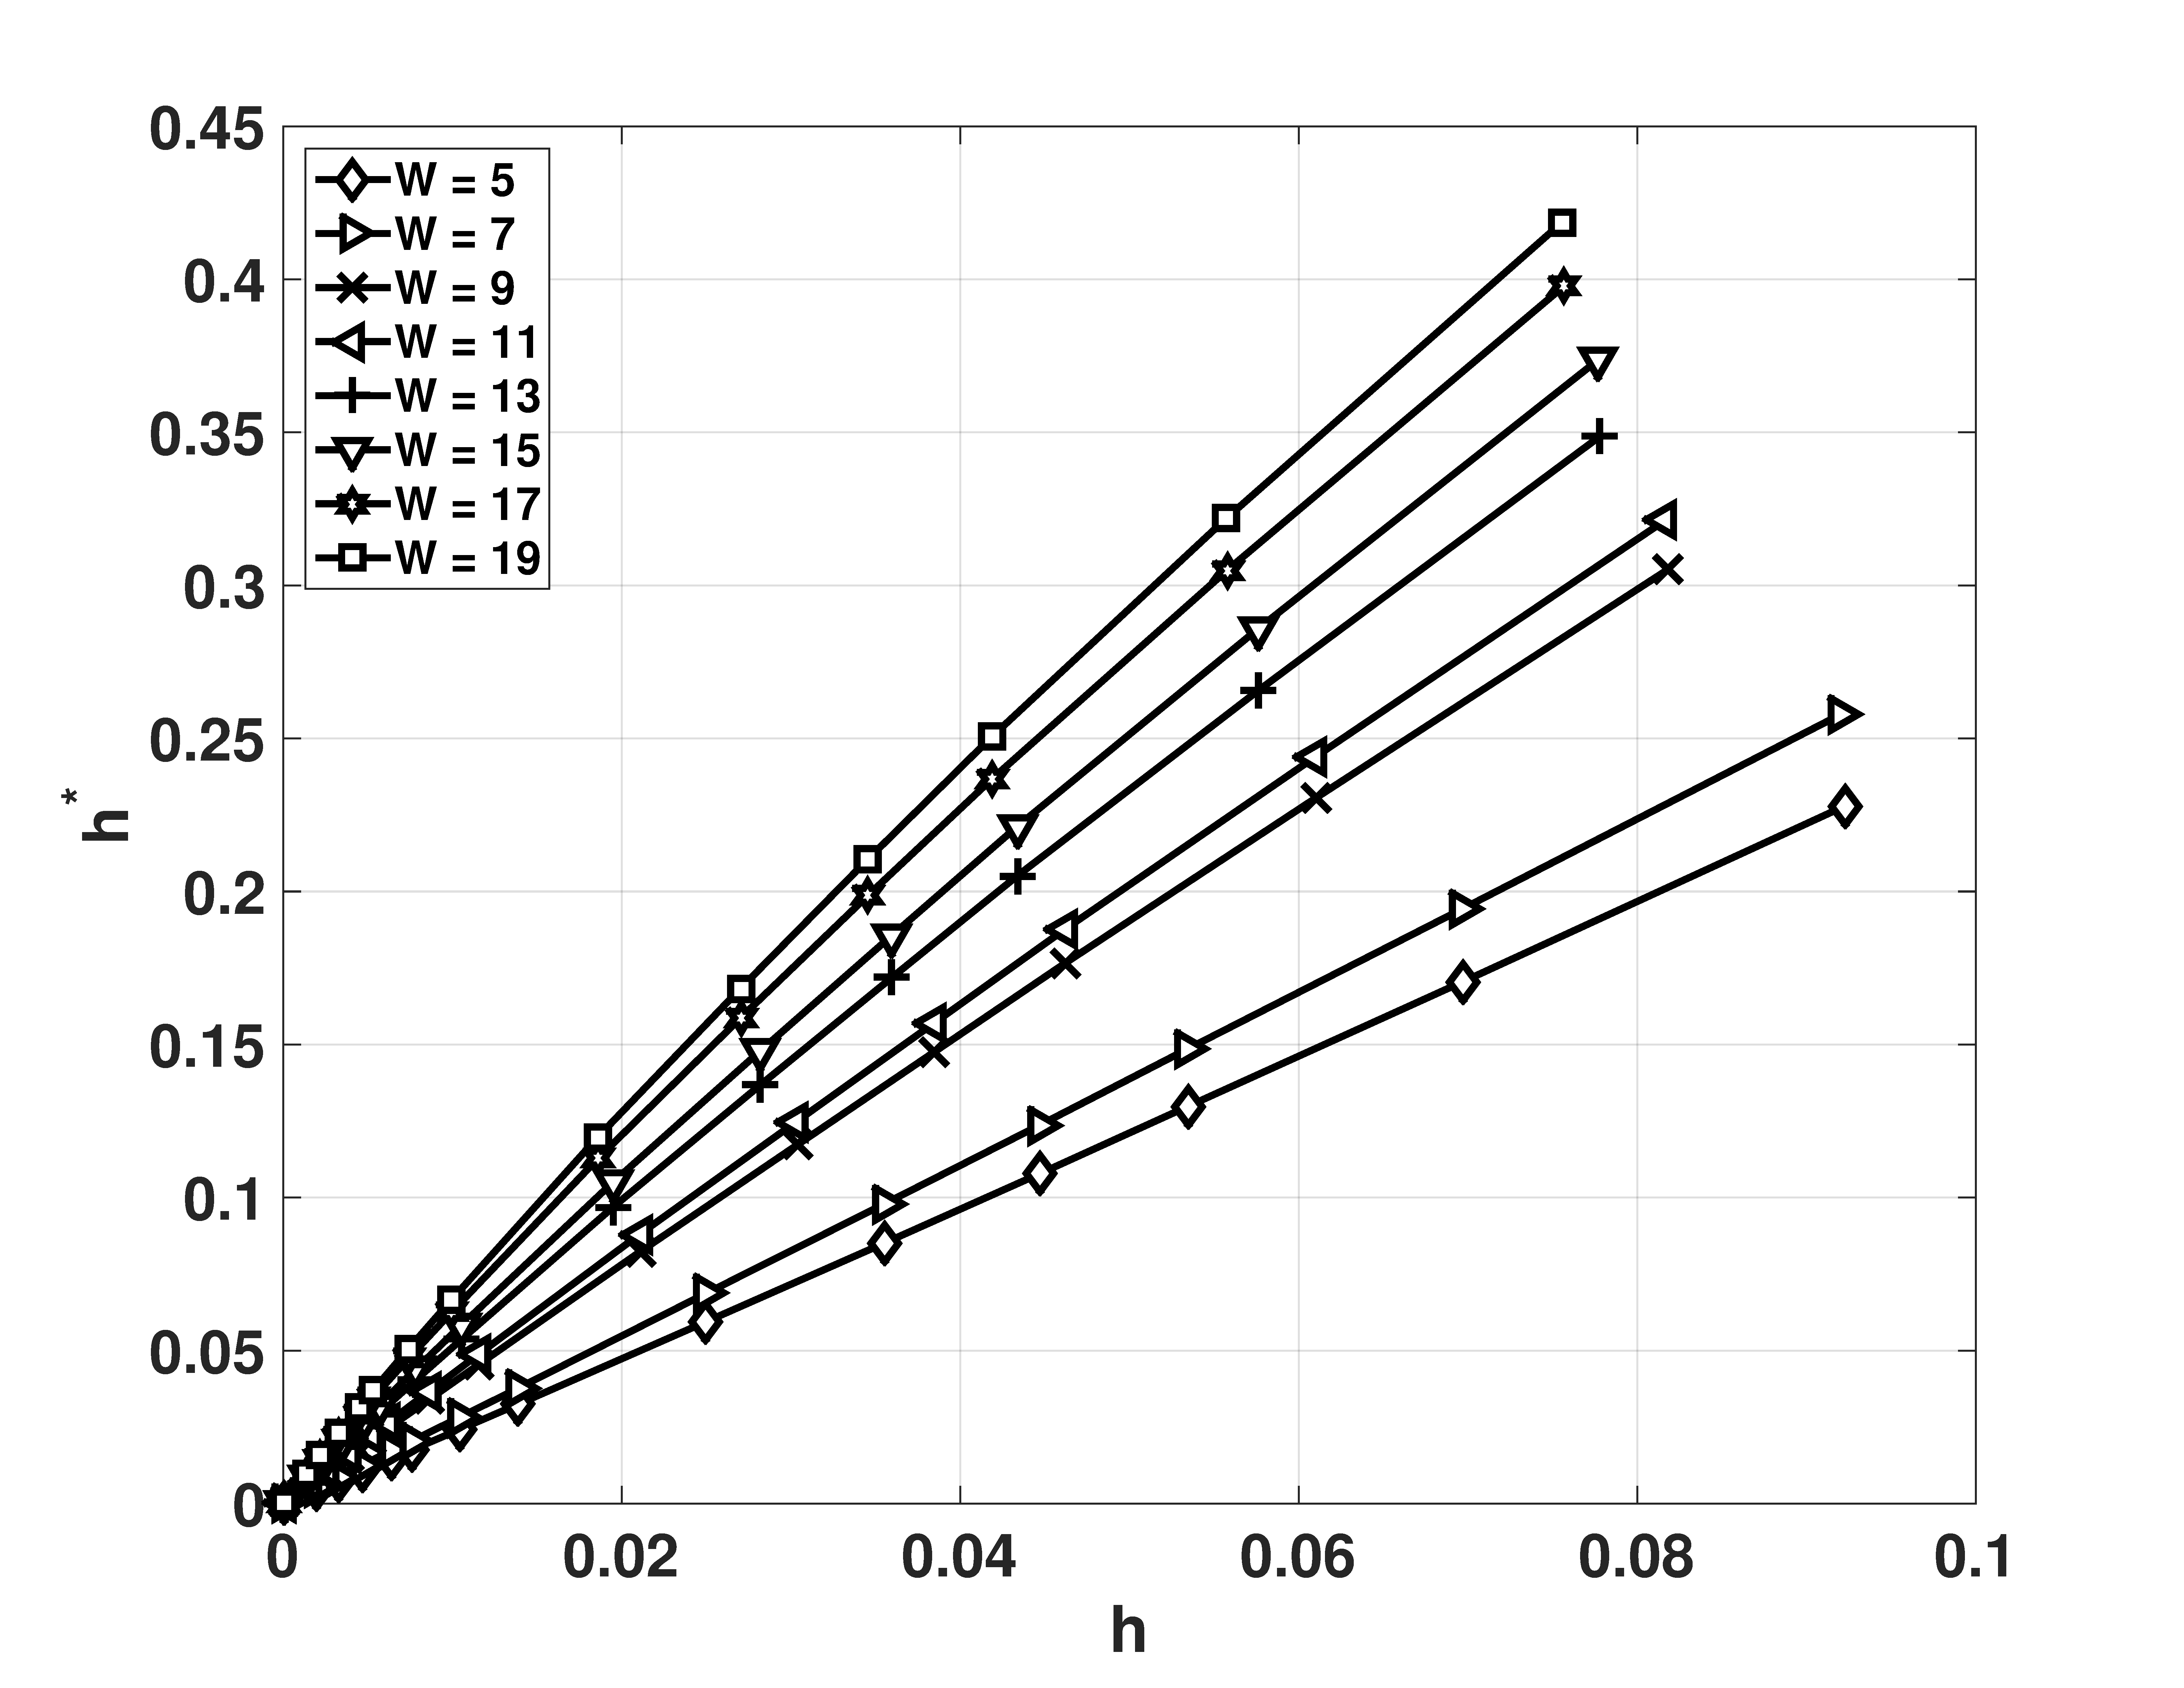
\includegraphics[ width=0.8\textwidth]{hm_h_CJ}
\caption{$h^*$ as a function of $h$ for $r=8$, $D=8$ and different values of $W$.}
\label{fig:hm_h_CJ}
\end{figure}

We also evaluated $h^*$ without the superposition of bits between consecutive natural numbers but keeping the superposition of $D-1$ natural numbers between ordering patterns (In all cases $h$ was evaluated with superposition of $W-1$ consecutive bits). Results are depicted in Fig. \ref{fig:Deltahm_Deltah_CS_SS} where it is shown that removing the superposition the sensitivity of this quantifier increases. Of course, we get a smaller amount of $W$ bits natural numbers form the original seven million binary file, and consequently, the statistical quality is lower than that of the original calculation with superposition. To increase $\alpha$ up to its previous value, longer binary files are required.

\begin{figure}
\center
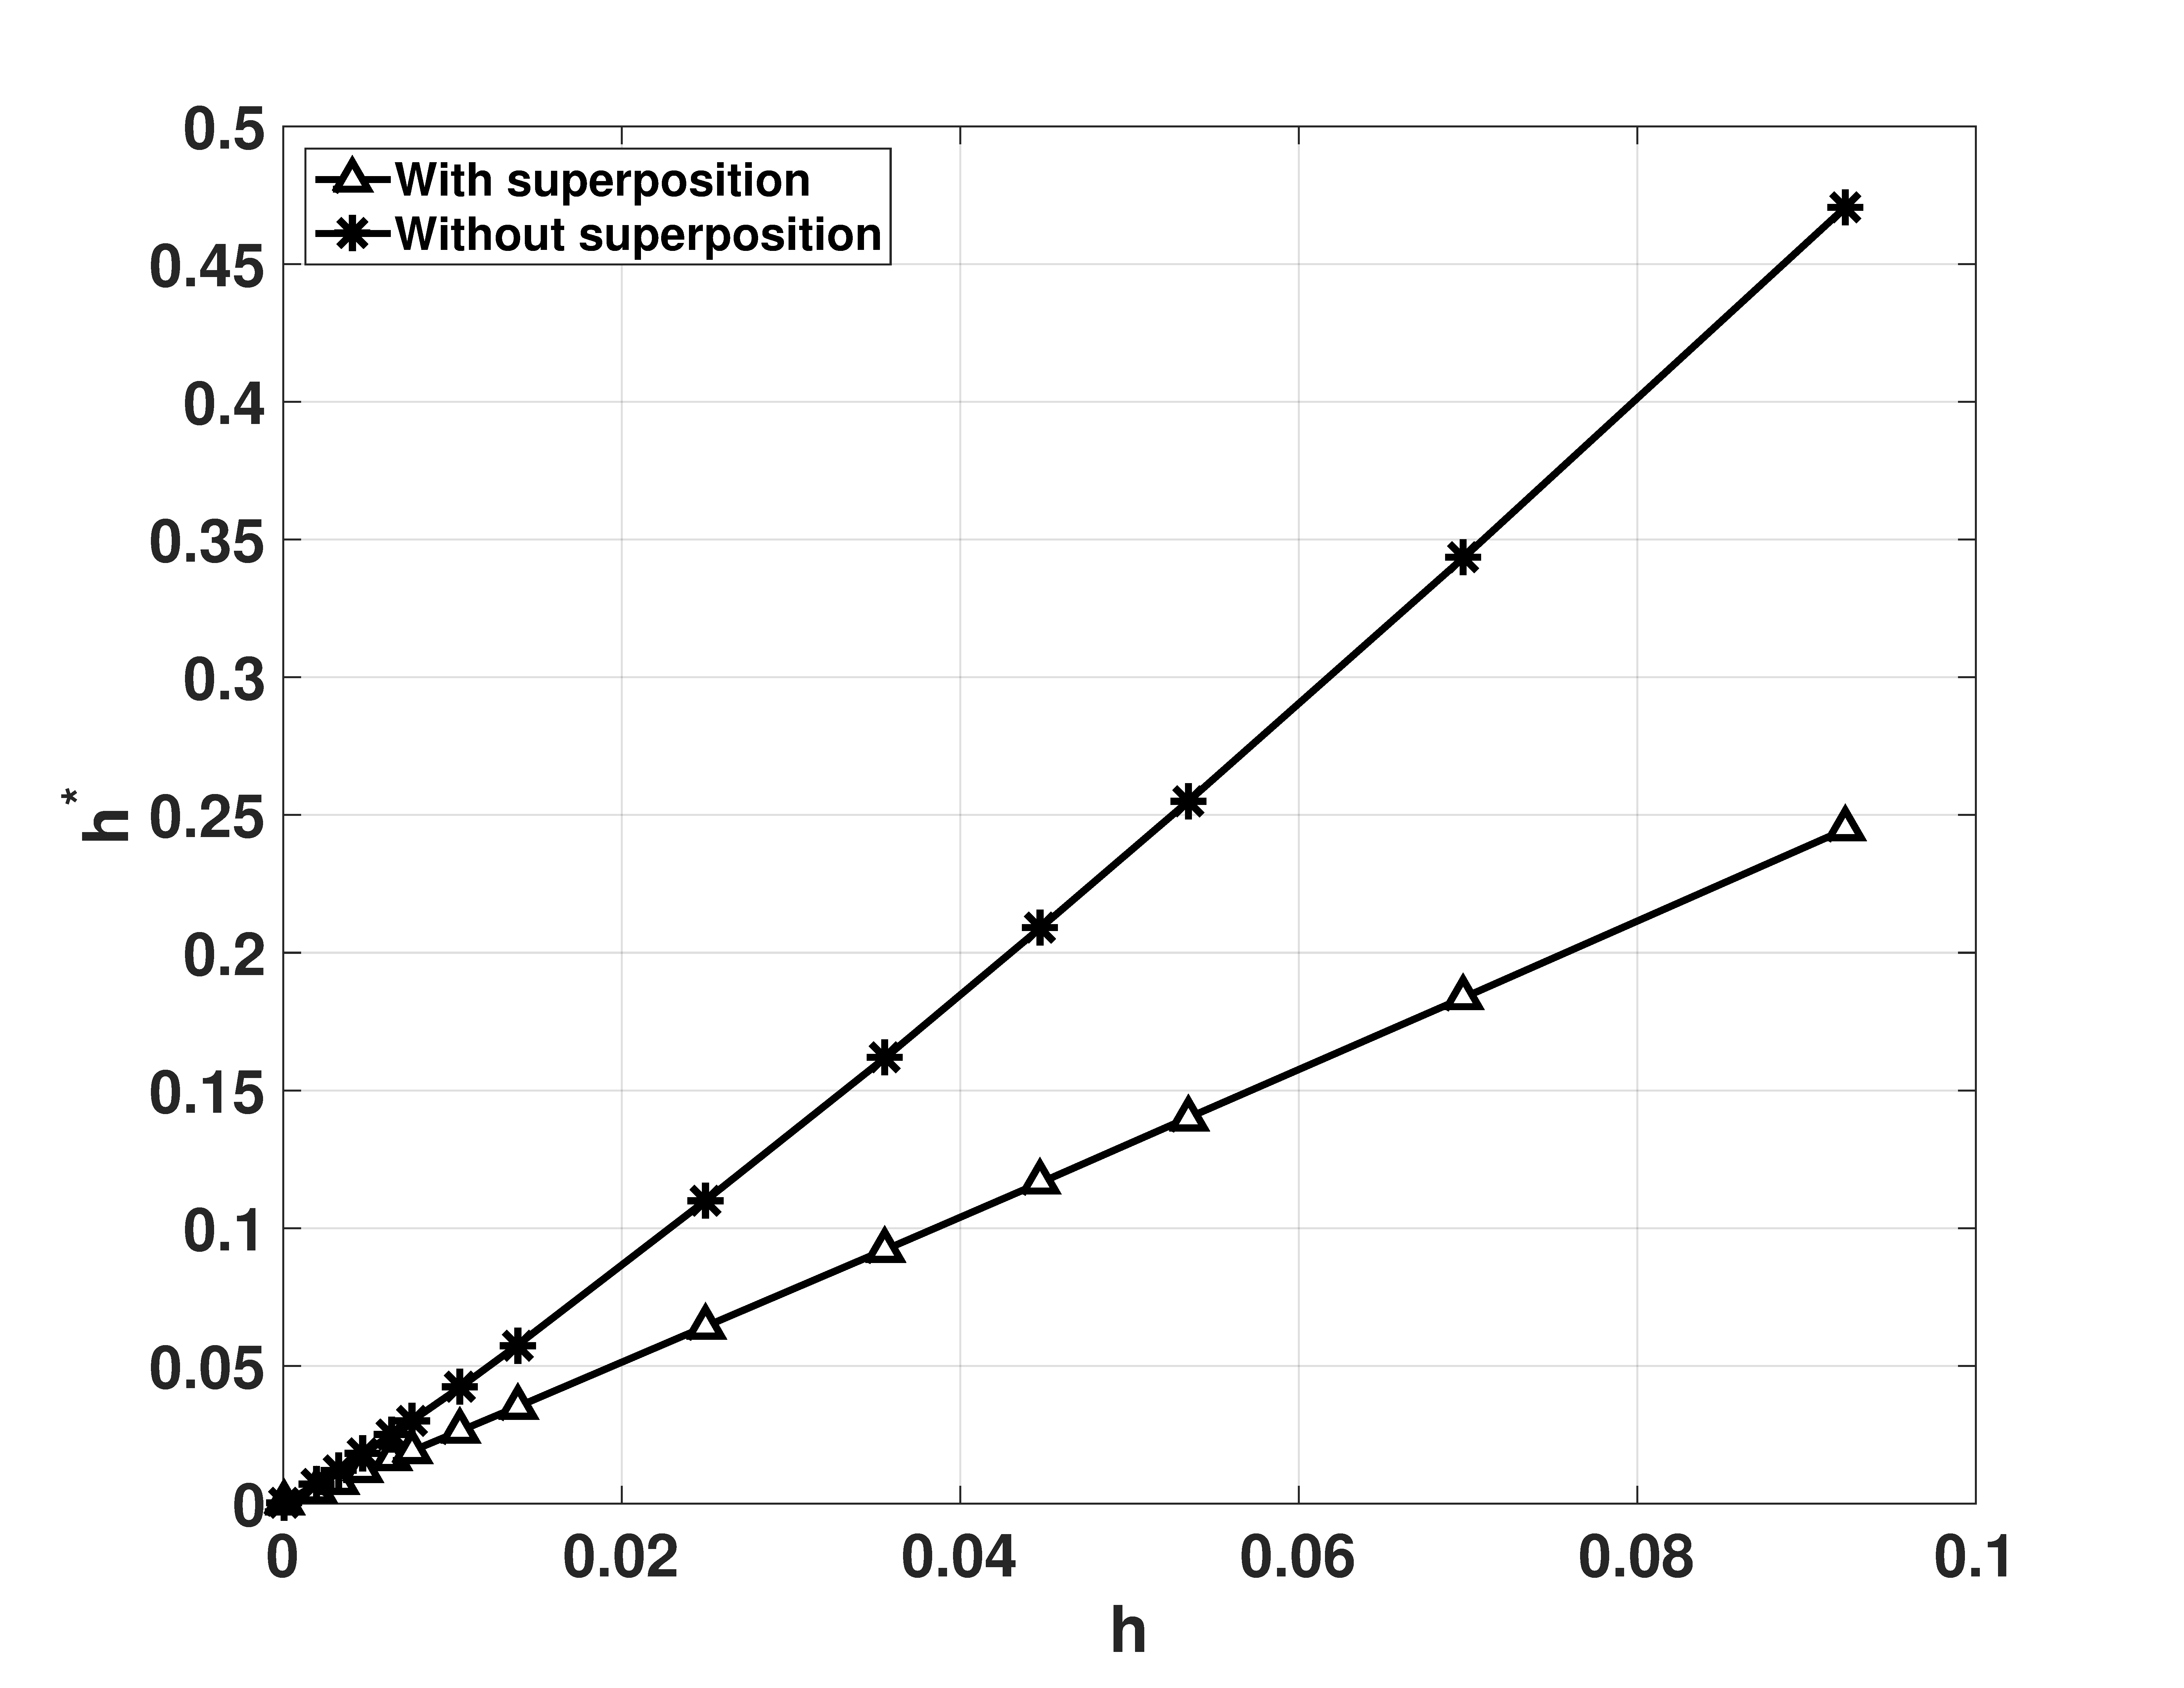
\includegraphics[ width=0.8\textwidth]{Deltahm_Deltah_CS_SS}
\caption{$h^*$ as a function of $h$ for $r=8$, $W=6$ and $D=8$. Two procedures to obtain $W$-bits natural numbers are considered: with and without superposition (see text).}
\label{fig:Deltahm_Deltah_CS_SS}
\end{figure}

\subsection{Conclusions}
\label{sec:conclu}
Given their usefulness as \emph{PRNG} and clock generators, \emph{RO}s are becoming one of the main building blocks of digital circuits. Jitter is unavoidable in \emph{RO}s, and consequently, it needs to be characterized. Mixing and distribution of values are the main properties to consider. 
Several \emph{ITQ} quantifiers were evaluated here. $S_W$, $S^{(D)}_{BP}$, $H_W$ and $H^{(D)}_{BP}$ turn out to be dependent on parameters $W$ and $D$. This is a drawback if we use them as jitter measures. On the other hand, it is no possible to calculate  \emph{rate entropies}, $h_0^*$ and $h_0$,  since an infinite number of data is necessary for their calculation. The two \emph{differential entropies}, $h^*$ and $h$, instead, are independent of the parameters used for their determination and are estimators of the \emph{rate entropies}. We have shown in Section \ref{sec:resu} that in the case of sampled \emph{RO}s they also present a minimum for the correct sampling ratio making them a good measure of the quality of both \emph{RO}'s and \emph{PRNG}'s derived from them. 

The dual entropy plane determined by these quantifiers has demonstrated to satisfactorily discern between the \emph{PRNG}'s two main desired properties, the equiprobability among all possible values and the statistical independence between consecutive values. Thus, it allows clearly seeing what needs to be improved in a given sequence.
The examples presented here have demonstrated the need to use both histograms for characterizing sequences.

%\bibliography{xbibMAXI_300314,xbibwebdiciembre2013_ingles}


%%%%%%%%%%%%%%%%%%%%%%%%%%%%%%%%%%%%%%%%%%%%%%%%%%%%%%%%%%%%%%%%%%%%%%%%%%%%%%%%%%%%%%%%%%%%%%%%%%%%%
\thispagestyle{empty}

\chapter{El problema de la Aritmética Discreta}

\section{Analysis of the digital implementation of a chaotic deterministic-stochastic attractor (EAMTA 2012)}

Otro que no tengo el latex, se lo tengo que pedir a Luciana

%test
In this work the implementation, of chaos-based
pseudo random number generators (PRNG), onto a Field Programmable Gate Array (FPGA), is analyzed. Any digital implementation requires the choice of an algorithm to discretize
time and a representation standard to represent real numbers.
Each choice modifies the stochasticity degree of the system and
also defines a different amount of resources on the FPGA. The
main contribution of this paper is to propose an optimum design
methodology for applications in which the chaotic system is going
to replace a stochastic system. This is the case with PRNG. In
stochastic systems the randomness degree must be measured. In
this paper we use the global indicator proposed by Marsaglia
in his widely used DIEHARD tests-suite. Results are exemplified
for the Lorenz chaotic oscillator but the same methodology may
be used with other low dimensional chaotic systems.

%%%%%%%%%%%%%%%%%%%%%%%%%%%%%%%%%%%%%%%%%%%%%%%%%%%%%%%%%%%%%%%%%%%%%%%%%%%%%%%%%%%%%%%%%%%%%%%%%%%%%%%%%%%%%%%%
\section{Complexity of switching chaotic maps}

\subsection{Introduction}
In the last years digital measuring systems become the standard in
all experimental sciences. By using \emph{virtual instruments} and new programable electronic
devices, such as Digital Signal Processors ($DSP$) and Field
Programmable Gate Arrays ($FPGA$)  experimenters may design and
modify their own measuring systems.

The effect of finite precision in these new devices needs to be
investigated. This issue is critical if  chaotic systems must be implemented, because due to roundoff errors digital implementations will always become periodic with a period $T$ and unstable orbits with a low period may become stable destroying completely the chaotic behavior.  
Grebogi and coworkers \cite{Grebogi1988} studied this subject and they shaw that the period $T$ scales with roundoff $\epsilon$ as
$T\sim\epsilon^{-d/2}$ where $d$ is the correlation dimension of
the chaotic attractor. 

To have a large period $T$ is one an important property of a chaotic map. Stochasticity and mixing are also relevant. Furthermore to characterize these properties several quantifiers were
studied  \cite{DeMicco2009}. Among them the use of an
entropy-complexity representation ($H-C$ plane) deserves special
consideration\cite{Rosso2007C,DeMicco2008,DeMicco2011,DeMicco2009,Rosso2009}. 
A fundamental issue is the criterium to select the distribution function ($PDF$) assigned to the time series. Causal and non causal options are possible. Here we consider the non-causal traditional $PDF$ obtained by normalization of the histogram of the time series. Its statistical quantifier is the normalized entropy$H_{hist}$ that is  a measure of equiprobability among all allowed values. We also consider a causal $PDF$  that is obtained by assigning ordering patterns to segments of trajectory of length $D$. This PDF were first proposed by Bandt \& Pompe in a seminal paper \cite{Pompe2002}. The corresponding entropy $H_{BP}$ was also proposed as a quantifier by Bandt \& Pompe. Amig\'o and coworkers proposed the number of forbidden patterns as a quantifier of chaos \cite{Amigo2007b}. Essentialy they reported the presence of forbidden patterns as an indicator of chaos. Recently it was shown that the name forbidden patterns is not convenient and it was replaced by  \emph{missing patterns}(MP) \cite{Rosso2012b}. 

Switching systems naturally arise in power electronics and many other areas in digital electronics. They have also interest in transport problems in deterministic ratchets \cite{Zarlenga2009} and it is known that synchronization of the switching procedure affects the output of the controlled system. Nagaraj et al \cite{Nagaraj2008} studied the case of switching between two maps. They shaw that the period $T$ of the
compound map obtained by switching between two chaotic maps is
higher than the period of each map.  Liu et al \cite{Liu2006} studied different switching rules applied to linear systems to generate chaos. Switching chaos was also addressed in \cite{Gluskin2008}.  Skipping values of the time series is another simple technique used to increase mixing in chaotic maps \cite{DeMicco2008}. 

In this paper we study the statistical characteristic of two well known maps: the tent map (TENT) and logistic map (LOG). Three additional maps are generated: 1) SWITCH, generated by switching between TENT and LOG; 2) EVEN, generated by skipping all the elements in odd position in SWITCH time series and 3) ODD, generated by discarding all the elements in an even position in SWITCH time series. Floating point, decimal numbers and binary numbers are used. All these specific numerical systems may be implemented in modern programmable logic boards. 

The main contributions of this paper are:
\begin{enumerate}
\item the definition of different statistical quantifiers and their relationship  with the properties of the time series generated by the map. 
\item the study of how this quantifiers are modified by the numerical representation using floating point, decimal and binary numbers. It is specially interesting to note that some systems (TENT) with very nice statistical properties in the world of the real numbers, become ``pathological" when numerical representations are used.
\item the effect of switching between two different maps, on the period and the statistical properties of the time series. Floating point, decimal and binary numerical representations are considered. 
\item the effect of skipping values in any of these maps
\end{enumerate}

Organization of the paper is as follows: section \ref{sec:quanti} describes the statistical quantifiers used in the paper and the relationship between their value and characteristics of the causal and non causal PDF considered; section \ref{sec:resultados} shows and discuss the results obtained for all the numerical representations. Finally section  \ref{sec:conclusions} deals with final remarks and future work. 
%
\subsection{Information theory quantifiers}\label{sec:quant}
The first step to quantify the statistical properties of the values (amplitude statistics) of a time series $\{x_i,~(i=1,...,N)\}$, using information theory is to determine the concomitant PDF because all the quantifiers are functionals of the PDF associated to the time series. This is an issue studied in detail in previous papers \cite{aka varios}. Let us summarize the procedure:
\begin{enumerate} 
\item \label{1} a finite alphabet  with $M$ symbols $\mathbf{ A}=\{a_1,...,a_M\}$ is chosen. 
\item \label{2} one of these symbols is assigned: (a) to each value of the time series of (b) to each portion of length $D$ of the trajectory. 
\item \label{3} the normalized histogram of the symbols is the desired $PDF$.
\end{enumerate}

Note that if option (a) is chosen in step \ref{2} then the PDF is \emph{non causal}, because all the information about the time evolution of the system generating $\{x_i\}$  is completely lost. On the contrary if option (b) is chosen in step \ref{2} then the PDF is \emph{causal}, in the sense it has some information about the temporal evolution.

 Of course there are infinite possibilities to choose the alphabet $\mathbf{ A}$ as well as the length $D$.
Bandt \& Pompe made a proposal for a causal PDF that has been shown to be easy to implement and useful in a great variety of applications.  The procedure is the
following \cite{Pompe2002,Keller2003,Keller2005}:
\begin{itemize}
\item Given a
series $\{x_t : t=0, \Delta t, \cdots,M\Delta t \}$, a sequence of
vectors of length $d$ is generated.

\begin{equation}
\label{eq:vectores}
(s)\mapsto \left(x_{t-(d-1)\Delta t},x_{t-(d-2)\Delta t},\cdots,x_{t-\Delta t},x_{t}\right) \ ,
\end{equation}

Each vector turns out to be the ``history'' of the value $x_t$.
Clearly, the longer the length of the vectors $D$, the more
information about the history would the vectors have but a higher value of $N$ is required to have an adequate statistics. 
\item The
permutations $\pi=(r_0, r_1, \cdots, r_{D-1})$ of $(0, 1, \cdots,
D-1)$ are called ``order of patterns'' of time $t$, defined by:

\begin{equation}
\label{eq:permuta}
x_{t-r_{D-1}\Delta t}\le x_{t-r_{D-2}\Delta t}\le\cdots\le x_{t-r_{1}\Delta t}\le x_{t-r_0\Delta t}.
\end{equation}
%
In order to obtain an unique result it is considered $r_i
<r_{i-1}$ if $x_{t-r_{i}\Delta t}=x_{t-r_{i-1}\Delta t}$.

In this way, all the $D!$ possible permutations $\pi$ of order
$D$, and the PDF $P=\{p(\pi)\}$ is defined as:

\begin{equation}
\label{eq:frequ}
p(\pi)~=~ \frac{\sharp \{s|s\leq M-D+1; (s) \quad \texttt{has type}~\pi\}}{M-D+1}.
\end{equation}
In the last expression the $\sharp$ symbol means ``number".
\end{itemize}
This procedure has the advantages of being {\it i)\/} simple, {\it
ii)\/} fast to calculate, {\it iii)\/} robust in presence of
noise, and {\it iv)\/} invariant to lineal monotonous
transformations.

It is applicable to weak stationarity processes (for
$k=D$, the probability that $x_t < x_{t+k}$ doesn't depend on the
particulary $t$ \cite{Pompe2002}).The causality property of the
PDF allows the quantifiers (based on this PDFs) to discriminate
between deterministic and stochastic systems \cite{Rosso2007B}.

According to this point Bandt and Pompe suggested $3\leq D \leq
7$. $D=6$ has been adopted in this work.

Based on our previous research \cite{DeMicco2008,DeMicco2009} we have employed two $PDF$'s: (a) the normalized histogram of the time series amplitudes $\{x_i\}$ (that is a non-causal $PDF$), and (b) the Bandt \& Pompe $PDF$ (that is a causal $PDF$).
The entropies $H_{hist}$ and $H_{BP}$, the statistical complexity $C_{BP}$  are used as quantifiers.  

We also used the number of missing patterns $MP$ as a quantifier\cite{Rosso2012}. As shown recently by Amig\'o {\it et al.\/}
\cite{Amigo2006,Amigo2007,Amigo2008,Amigo2010},  in the case of
deterministic one-dimensional maps, not all the possible ordinal patterns
can be effectively materialized into orbits, which in a sense
makes these patterns ``forbidden". Indeed, the existence of these
{\it forbidden ordinal patterns\/} becomes a persistent fact that
can be regarded as a ``new" dynamical property. Thus, for a fixed
pattern-length (embedding dimension $D$) the number of forbidden
patterns of a time series (unobserved patterns) is independent of
the series length $N$. Remark that this independence does not
characterize other properties of the series such as proximity and
correlation, which die out with time \cite{Amigo2007,Amigo2010}.

A full discussion about the convenience of using these quantifiers is
out of the scope of this work. Nevertheless reliable bibliographic
sources do exist
\cite{Wackerbauer1994,Lopez1995,Rosso2007A,DeMicco2008,Rosso2009,Martin2006,Rosso2012}.

The entropies $H_{hist}$ and $H_{BP}$ are the normalized version of the  Of course there are infinite possibilities to choose the alphabet as well as the length $d$.
Bandt \& Pompe made a proposal for a causal PDF that has been shown to be easy to implement and useful in a great variety of applications.  The procedure is the
following \cite{Pompe2002,Keller2003,Keller2005}: a) Given a
series $\{x_t : t=0, \Delta t, \cdots,M\Delta t \}$, a sequence of
vectors of length $d$ is generated.

\begin{equation}
\label{eq:vectores}
(s)\mapsto \left(x_{t-(d-1)\Delta t},x_{t-(d-2)\Delta t},\cdots,x_{t-\Delta t},x_{t}\right) \ ,
\end{equation}

Each vector turns out to be the ``history'' of the value $x_t$.
Clearly, the longer the length of the vectors $d$, the more
information about the history would the vectors have. b) The
permutations $\pi=(r_0, r_1, \cdots, r_{d-1})$ of $(0, 1, \cdots,
d-1)$ are called ``order of patterns'' of time $t$, defined by:

\begin{equation}
\label{eq:permuta}
x_{t-r_{d-1}\Delta t}\le x_{t-r_{d-2}\Delta t}\le\cdots\le x_{t-r_{1}\Delta t}\le x_{t-r_0\Delta t}.
\end{equation}
%
In order to obtain an unique result it is considered $r_i
<r_{i-1}$ if $x_{t-r_{i}\Delta t}=x_{t-r_{i-1}\Delta t}$.

In this way, all the $d!$ possible permutations $\pi$ of order
$d$, and the PDF $P=\{p(\pi)\}$ is defined as:

\begin{equation}
\label{eq:frequ}
p(\pi)~=~ \frac{\sharp \{s|s\leq M-Dd+1; (s) \quad \texttt{has type}~\pi\}}{M-d+1}.
\end{equation}
In the last expression the $\sharp$ symbol means ``number".

This procedure has the advantages of being {\it i)\/} simple, {\it
ii)\/} fast to calculate, {\it iii)\/} robust in presence of
noise, and {\it iv)\/} invariant to lineal monotonous
transformations.

It is applicable to weak stationarity processes (for
$k=d$, the probability that $x_t < x_{t+k}$ doesn't depend on the
particulary $t$ \cite{Pompe2002}).The causality property of the
PDF allows the quantifiers (based on this PDFs) to discriminate
between deterministic and stochastic systems \cite{Rosso2007B}.

The choice of the embedding dimension $d$ is crucial because it
determines the minimal length acceptable of the original temporal
series ($M \gg d!$) needed to obtain an adequate statistics.
According to this point Bandt and Pompe suggested $3\leq d \leq
7$. $d=6$ has been adopted in this work.

Based on our previous research \cite{DeMicco2009} we have employed
the statistical complexity $C$ and the entropy $H$ to define a plane where the stochasticiy of the chaotic system may be represented. A full discussion about the convenience of using these quantifiers is
out of the scope of this work. Nevertheless reliable bibliographic
sources do exist
\cite{Wackerbauer1994,Lopez1995,Rosso2007A,DeMicco2008,Rosso2009,Martin2006}.

The entropy $H[P]$ is the normalized version of the Entropy proposed by Shannon \cite{Shannon1949a}:
\begin{equation}\label{eq:sha}
H[P] = S[P] /S_{max},
\end{equation}
where $S[P]=-\sum _{j=1}^{M}~p_j~\ln( p_j )$\\ and $S_{max}$ is
the normalizing constant:
\begin{equation}
\label{eq:Smax} S_{max}= S[P_e] = \ln M,
\end{equation}
and $P_e=\{ 1/M, \cdots,1/M\}$ is the uniform distribution. The number of symbols $M$ is equal to $N$ for $H_{hist}$ and it is equal to $D!$ for $H_{BP}$.

The statistical complexity $C[P]$ is given by:
\begin{equation}
\label{eq:inten}
C[{P}]=Q_{J}[{P,P_e}]\cdot H[{P}] \ ,
\end{equation}
, and
$Q_{J}$ is named ``disequilibrium'' and it is the distance between $P$ and $P_e$ 
 in the probability space. The metric used in this paper is based on the Jensen-Shannon divergence
 \cite{Lamberti2004}:
\begin{equation}
\label{eq:disequi}
Q_{J}[{P,P_e}]= Q_0 \cdot \{S[\frac{P+P_e}{2}]-S[P]/2-S[P_e]/2 \} \ .
\end{equation}
The normalization constant $Q_0$ is:
\begin{equation}
\label{eq:q0j}
Q_0=-2 \left\{ \left( \frac{N+1}{N} \right) \ln(N+1) - 2 \ln(2N) + \ln N \right\}^{-1} .
\end{equation}

From the statistical point of view the disequilibrium $Q_J$ is an
intensive magnitude, and it is $0$ if and only if $P=P_e$. It has
been proved that the $C[P]$ quantifies the presence of nonlinear
correlations typical of chaotic systems
\cite{Martin2003,Lamberti2004}. The complexity $C[P]$ is
independent from the entropy $H[P]$, as far as different $P$'s share
the same entropy $H[P]$ but they have different  complexity
$C[P]$.

Two representation planes are considered: $H_{BP}$ vs $H_{hist}$ \cite{DeMicco2008} and $H_{BP}$ vs $C_{BP}$ \cite{Rosso2007C}. In the first plane a higher value in any of the entropies,  $H_{BP}$ and $H_{hist}$, implies an increase in the uniformity of the involved $PDF$. The point $(1,1)$ represents the ideal case with uniform histogram and uniform distribution of ordering patterns.  In the second plane not the entire region $0<H_{BP}<1$, $0<C_{BP}<1$ is achievable. In fact for any $PDF$ the pairs $(H,C)$ of possible values fall between two extreme curves in the plane $H$-$C$ \cite{Anteneodo1996}. Fig. \ref{fig:planezone} shows two regions labeled as \emph{deterministic} and \emph{stochastic}. In fact transition from one region to the other are smooth and the division is a bit arbitrary. A more detailed discussion can be seen in \cite{Rosso2007C}. Ideal random systems having uniform Bandt \& Pompe $PDF$, are represented by the point $(1,0)$ \cite{Gonzalez2005} and a delta-like $PDF$ corresponds with the point $(0,0)$. 


%
\subsection{Results}\label{sec:resultados}
Five pseudo chaotic maps were studied. For each one a floating point representation, a decimal numbers representation with $1\leq P \leq 27$ and a binary numbers representation with $1\leq B \leq 27$ are considered. For each representation $1000$ time series were generated using randomly chosen initial conditions within the interval $[0,1]$. 
The studied maps are tent (TENT), logistic (LOG) a sequential switching between TENT and LOG (SWITCH). Furthermore a skipping randomization procedure is applied to SWITCH \cite{DeMicco2008}, discarding the values in the odd positions (EVEN) or the values in the even positions (ODD) respectively. Let us detail our results for each of these maps. 
\subsection {Simple maps.}\label{subsec:simples}
Here we report our results for both maps:
\begin{enumerate}
%
\item Tent map (TENT)
\begin{equation}\label{eq:tentmap}
x_{n+1}~=~ \left\{ \begin{array}{ll}
2~{x_n} & \textrm{if ~$0\leq x_n\leq 1/2$}\\
2~(1-{x_n}) & \textrm{if ~$1/2<x_n\leq 1$} 
\end{array} \right.  \ ,
\end{equation}
with $x_n\in\mathcal{R}$.
%
The Tent map has been extensively studied in the literature because theoretically it has nice  statistical properties that can be analytically obtained. For example it is easy to proof that it has a uniform histogram and consequently an ideal $H_{hist}=1$. The Perron-Frobenius operator and its corresponding eigenvalues and eigenfunctions may be also be analytically obtained for this map \cite{tent}. 

When this map is implemented in a computer using any numerical representation system (even floating point!) truncation errors rapidly increases and makes the unstable fixed point in $x^*=0$ becomes stable producing a short transitory followed by an infinite number of  $0$'s\cite{Jessa1993,Callegari1997}. Some authors \cite{buscar} have proposed to add a random perturbation to avoid this drawback of the Tent map. But this procedure introduces statistical properties of the random perturbation that are mixed with those of the Tent map itself.

Here we study the Tent map ``as it is«« without any artifact to evaluate its real instead of theoretical statistical properties. Note that to effectively work in a given representation it is necessary to change the expression of the map in order to make all the operations in the chosen representation numbers. For example, in the case of TENT the expression in decimal numbers is:

\begin{equation}\label{eq:tentdecbin}
x_{n+1}~=~ \left\{ \begin{array}{ll}
2~{x_n} & \textrm{if $0\leq x_n\leq 1/2$}\\
\epsilon \times floor\{\frac{2~-~2~x_n}{\epsilon}\} & \textrm{if $1/2<x_n\leq 1$} 
\end{array} \right.  \ ,
\end{equation}
with $\epsilon=10^{-P}$ for decimal numbers and $\epsilon=2^{-B}$ for binary numbers. In Eq. \ref{eq:tentdecbin} $x_n$ is either a decimal number with $P$ digits or a binary number with $B$ bits.

Figs. \ref{fig:tent} (a) to (e) show the different quantifiers for floating point and decimal numerical representation. In each figure from (a) to (c) a dashed line shows the value for the floating point representation. In figures (d) and (e) the star corresponds to the floating point case. In decimal representations the value of $H_{hist}$ remains almost constant for $11\leq P\leq 16$ (see Fig. \ref{fig:tent} (a)). Its value is $<H_{hist}>=0.8740$ with a variance $\sigma_{Hhist}=2.5 \times 10^{_6}$. For lower or higher values pf $P$ entropy decreases. This effect is due precisely to the stabilization of the fixed point at $x=0$. For ordering patterns entropy $H_{BP}$ an almost constant value is obtained for $8\leq P \leq 15$. The value is  $H_{BP}\simeq 0.6287$ with variance $\sigma_{H_{BP}}=4.8 \times 10^{-6}$ (see Fig. \ref{fig:tent} (b)). This rather small maximum value may be understood by seeing  Fig. \ref{fig:tent} (c), where the number of MP.
% 
is minimal for $P$ within the same range but it is still large: $645$ patterns are missing and only $75$ ordering patterns are present in the time series. Then, even with a uniform distribution between these $75$ patterns, entropy can not be higher than $ln(75)/ln(720)\simeq 0.65$. 
A more complete perspective of the statistical properties is obtained in Fig. \ref{fig:tent} (d) showing the representative point in the $H_{hist},H_{BP}$ plane for different precisions. Note that the best choice for maximum stochasticity is obtained for $11\leq P \leq 15$, with maximum attainable values for both entropies.
Increasing the number of decimal figures makes Tent map worst in the sense the system approaches the state for the floating point representation (the star at $(0,0)$. 
Statistical complexity $C_{BP}$ is also maximal for $8\leq P \leq 15$. 
Fig. \ref{fig:tent} (e) shows the representation on the $H_{BP},C_{BP}$ plane. In this plane it is also clear that the more stochastic option corresponds with  $11\leq P \leq 15$ but even in the optimum case the representative point is located in a position very similar to other chaotic maps, very far from the ideal point for stochastic systems in this plane that is $(1,0)$ \cite{Rosso2007C}.
Binary numerical representation of the Tent map remains very near to the floating point values for  $1 \leq B \leq 27 $ (see Fig. \ref{fig:tent} (f)).
The conclusion is it is convenient to use a decimal numbers representation with  $P=11$ to get the optimum time series for the Tent map. A higher number of decimal figures does not improve the statistical properties of the time series. Furthermore binary and floating point representations are not allowed. 
%
\item Logistic map (LOG)
Logistic map is representative of the very large family of quadratic maps. 
\begin{equation}\label{eq:logimap}
 x_{n+1}~=~4~x_n~(1-x_n) \ ,
\end{equation}
with $x_n\in\mathcal{R}$.
%
Figs. \ref{fig:LOGdecimal} (a) to (f) show the statistical properties of LOG map in floating point and decimal numbers representation. This map does not show the anomalies pointed above for the tent map. For $P\geq 10$ the values of $H_{hist}$, $H_{BP}$ and $C_{BP}$ remains almost identical to the values for the floating point representation. Their values are: $<H_{hist}>=0.8621$ with variance $\sigma_{H_{hist}}=0.062 \times 10^{-6}$; $<H_{BP}>=0.6292$ with variance $\sigma_{H_{BP}}=0.060 \times 10^{-6}$; $<C_{BP}>=0.4842$ with variance $\sigma_{C_{BP}}=0.0195 \times 10^{-6}$. Missing patterns stabilize in $645$ for $P \geq 8$ making $H_{BP}$ to rise to its floating point value $<H_{BP}>=0.629$ with variance $\sigma_{H_{BP}}=0.060 \times 10^{-8}$. Note again that the stable value of mission patters missing patterns $645$ makes the optimum $H_{BP} \leq ln(75)/ln(720) \simeq 0.65$. Then $P=10$ is the most convenient choice because an increase in the number of decimal figures does not improve the statistical properties. 
Figs. \ref{fig:LOGbin} show the corresponding figures for binary representations. The histogram entropy $H_{hist}$ does not reach its floating point value within the maximum number of bits used. In the case of missing patterns the stable number $645$ is obtained with $B \geq 25$. It means that using $B=25$ one obtains a time series with good statistical properties regarding the missing patterns, but distribution among the allowed binary values is not as uniform as can be obtained with a higher value of $B$. 
\end{enumerate}

In summary, a comparison between LOG and TENT maps shows that, in the case of decimal representation, the best choice for TENT ($P=11$) produces a higher value for $H_{hist}$ than the best choice for LOG ($P=10$). Ordering patterns and the statistical properties related to them, are almost identical for the optimum choices in both maps. In the case of binary numbers  only LOG  can be used because TENT is highly anomalous. 

\subsubsection{Sequential switching}
\begin{enumerate}
\item Sequential switching between Tent and Logistic maps (SWITCH)
SWITCH may be expressed as a composition between $M_1 \circ M_2$ given by the following recurrence:
%
\[ \left\{ \begin{array}{ccc}\label{eq:seq}
x_{n+2}~=~ 4~x_{n+1}~(1-{n+1}) \\
x_{n+1}~=~ \left\{ \begin{array}{ll}
2~{x_n} & \textrm{if $0\leq x_n\leq 1/2$}\\
2~(1-{x_n}) & \textrm{if $1/2<x_n\leq 1$} 
\end{array} \right.  \end{array}\right. \] 
with $x_n\in\mathcal{R}$.
%
Results with sequential switching are shown in Figs. \ref{fig:seqdec} (a) to (f) for decimal numbers. The floating point entropy value is $H_{hist}=0.8658$, a value very similar to the one obtained for the TENT map and higher to that obtained for LOG. For decimal numbers this value is reached for $12 \leq P \leq 27$. It means it is enough to use $12$ decimal figures to get the same distribution of values in the time series. Regarding ordering patterns the number of MP decreases to $586$, a value lower lower than the one obtained for any of two simple maps TENT and LOG. It means the entropy $H_{BP}$ may increase up to $ln(134)/ln(720)\simeq 0.74$ With decimal numbers the entropy $H_{BP} $stabilizes at $P=9$ with $<H_{BP}>\simeq 0.657$ and variance $\sigma_{H_{BP}} \simeq 0.13 \times 10^{-7}$. Note that the entropies $H_{hist}$ and $H_{BP}$ are not monotonously increasing with $P$.  Considering all the quantifiers $P=12$ is the minimum number of decimal figures and statistical characteristics of this combined map are better than those for each individual map.
%
Results with sequential switching in binary numbers are shown in Figs. \ref{fig:seqbin}. Results for a number of bits $B\simeq27$ are equivalent to those obtained for $P\simeq 9$ for decimal numbers. It means both representation are valid and equivalent in the sense they will require similar hardware resources. 
\item 
Skipping is a usual randomizing technique that increases the mixing quality of a single map and correspondingly increases the value of $H_{BP}$ and decreases $C_{BP} $ of the time series. Skipping does not change the values of $H_{hist}$ and $C_{hist}$ evaluated using the non causal PDF (normalized histogram)\cite{DeMicco2008}. In the case under consideration we study Even and Odd skipping of the sequential switching of Tent and Logistic maps.
\begin{enumerate}
\item Even skipping of the sequential switching of Tent and Logistic maps (EVEN).\\
If $\{x_n,~(n=1,...\infty)\}$ is the time series generated by \ref{eq:seq} discard all the values in odd positions and retain the values in even positions.
\item Odd skipping of the sequential switching of Tent and Logistica maps.
If $\{x_n,~(n=1,...\infty)\}$ is the time series generated by \ref{eq:seq} discard all the values in even positions and retain all the values in odd positions.

The reason for studying even and odd skipping cases is the sequential switching map $M_{switch}$ is the composition of two different maps. Even skipping may be expressed as $M_{TENT}\circ M_{LOG}$ while odd skipping may be expressed as $M_{LOG}\circ M_{TENT}$.
\end{enumerate}
This is very interesting to note that a great improvement is obtained using any of the skipping strategies but EVEN is slightly better than ODD.  

MP are reduced to $MP\simeq 163$ for EVEN and $MP\simeq 164$ for ODD, increasing the maximum allowed Bandt \& Pompe entropy that reaches the mean value $<H_{BP}>\simeq 0.905$ with variance $\sigma_{H_{BP}}\simeq=0.107 \times 10^{-6}$ for EVEN, and $<H_{BP}>\simeq 0.854$ with variance $\sigma_{H_{BP}}\simeq=0.285 \times 10^{-6}$ for a decimal representation with  $9\leq P\leq27$. The complexity is reduced to $<C_{BP}>\simeq 0.224$ with $\sigma_{C_{BP}}\simeq=0.166 \times 10^{-6}$ for EVEN and  $<C_{BP}>\simeq 0.282$ with $\sigma_{C_{BP}}\simeq=0.281 \times 10^{-6}$ for ODD.

Quantifiers related to the normalized histogram slightly degrades with the skipping procedure. For example $H_{hist}$ reduces from $0.866$ without skipping to $0.813$ for any EVEN or ODD. 

Results in binary numbers are similar to those obtained for the equivalent number of figures in decimal numbers. For example the minimum in MP is reached for $B=27$, and this number of bits is almost equivalent to $P=9$. 
\end{enumerate}
In Figs. \ref{fig:seqpardec} and Figs. \ref{fig:seqparbin} are shown the results for EVEN. We do not give the Figs. for ODD because they are very similar, as pointed above. 
%
\subsubsection{Period $T$ as a function of $P$ and $B$}
The issue of how the period $T$ is related with the representation with $P$ decimal digits was studied by Grebogi and coworkers \cite{Grebogi1988}. There they shaw that the period $T$ scales with roundoff $\epsilon$ as
$T\sim\epsilon^{-d/2}$ where $d$ is the correlation dimension of
the chaotic attractor. Nagaraj et al \cite{Nagaraj2008} studied the case of switching between two maps. They shaw that the period $T$ of the
compound map obtained by switching between two chaotic maps is
higher than the period of each map and they found that a ''random" switching improves the results. Here we considered  sequential switching to avoid the use of another random variable, because it can include its own statistical properties in the time series. We studied decimal and binary numbers representations. Fig. \ref{fig:peril} shows  $T$ vs $P$ in semi logarithmic scale. 
% OJO ACA REVISAR SI ESTA BIEN
A straight line can fit the points and has the expression  $log_{10}T=m \times P + b$ for decimal numbers and  $log_{2}T=m \times B + b$ for binary numbers, where $m$ is the slope and $b$ is the $y$-intercept. Results for all considered maps are summarized in Table \ref{tabla:tab1} and \ref{tabla:tab2}.

\begin{table}
% table caption is above the table
\caption{Period $T$ as a function of $P$ for the maps considered}
\label{tabla:tab1}       % Give a unique label
% For LaTeX tables use
\begin{tabular}{lll}
\hline\noalign{\smallskip}
map & m & b  \\
\noalign{\smallskip}\hline\noalign{\smallskip}
TENT&0.436 & -0.0705 \\
LOG &0.422 & 0.0141 \\
SWITCH &0.438 & 0.0276 \\
EVEN &0.438 & -~0.2734 \\
ODD &0.438 & -~0.2734 \\
\noalign{\smallskip}\hline
\end{tabular}
\end{table}
%
\begin{table}
% table caption is above the table
\caption{Period $T$ as a function of $B$ for the maps considered}
\label{tabla:tab2}       % Give a unique label
% For LaTeX tables use
\begin{tabular}{lll}
\hline\noalign{\smallskip}
map & m & b  \\
\noalign{\smallskip}\hline\noalign{\smallskip}
TENT&- & - \\
LOG &0.494 & -1.219 \\
SWITCH &0.494 & -0.871 \\
EVEN &0.494 & -1.871 \\
ODD &0.494 & -1.871 \\
\noalign{\smallskip}\hline
\end{tabular}
\end{table}
Results are compatible for those obtained in \cite{Nagaraj2008}. Switching between maps increase de period $T$ but the skipping procedure decrease it esentially to one half. 
% 

\subsection{Conclusions}\label{sec:conclusions}
In summary:
\begin{itemize}
  \item 
  \item 
  \item 
\end{itemize}produces a non-monotonous evolution toward the floating point result. This result is relevant because it shows that increasing the precision is not
always recommended.


%%%%%%%%%%%%%%%%%%%%%%%%%%%
% FIGURAS
%%%%%%%%%%%%%%%%%%%%%%%%%%% Fig.0
%
\begin{figure}
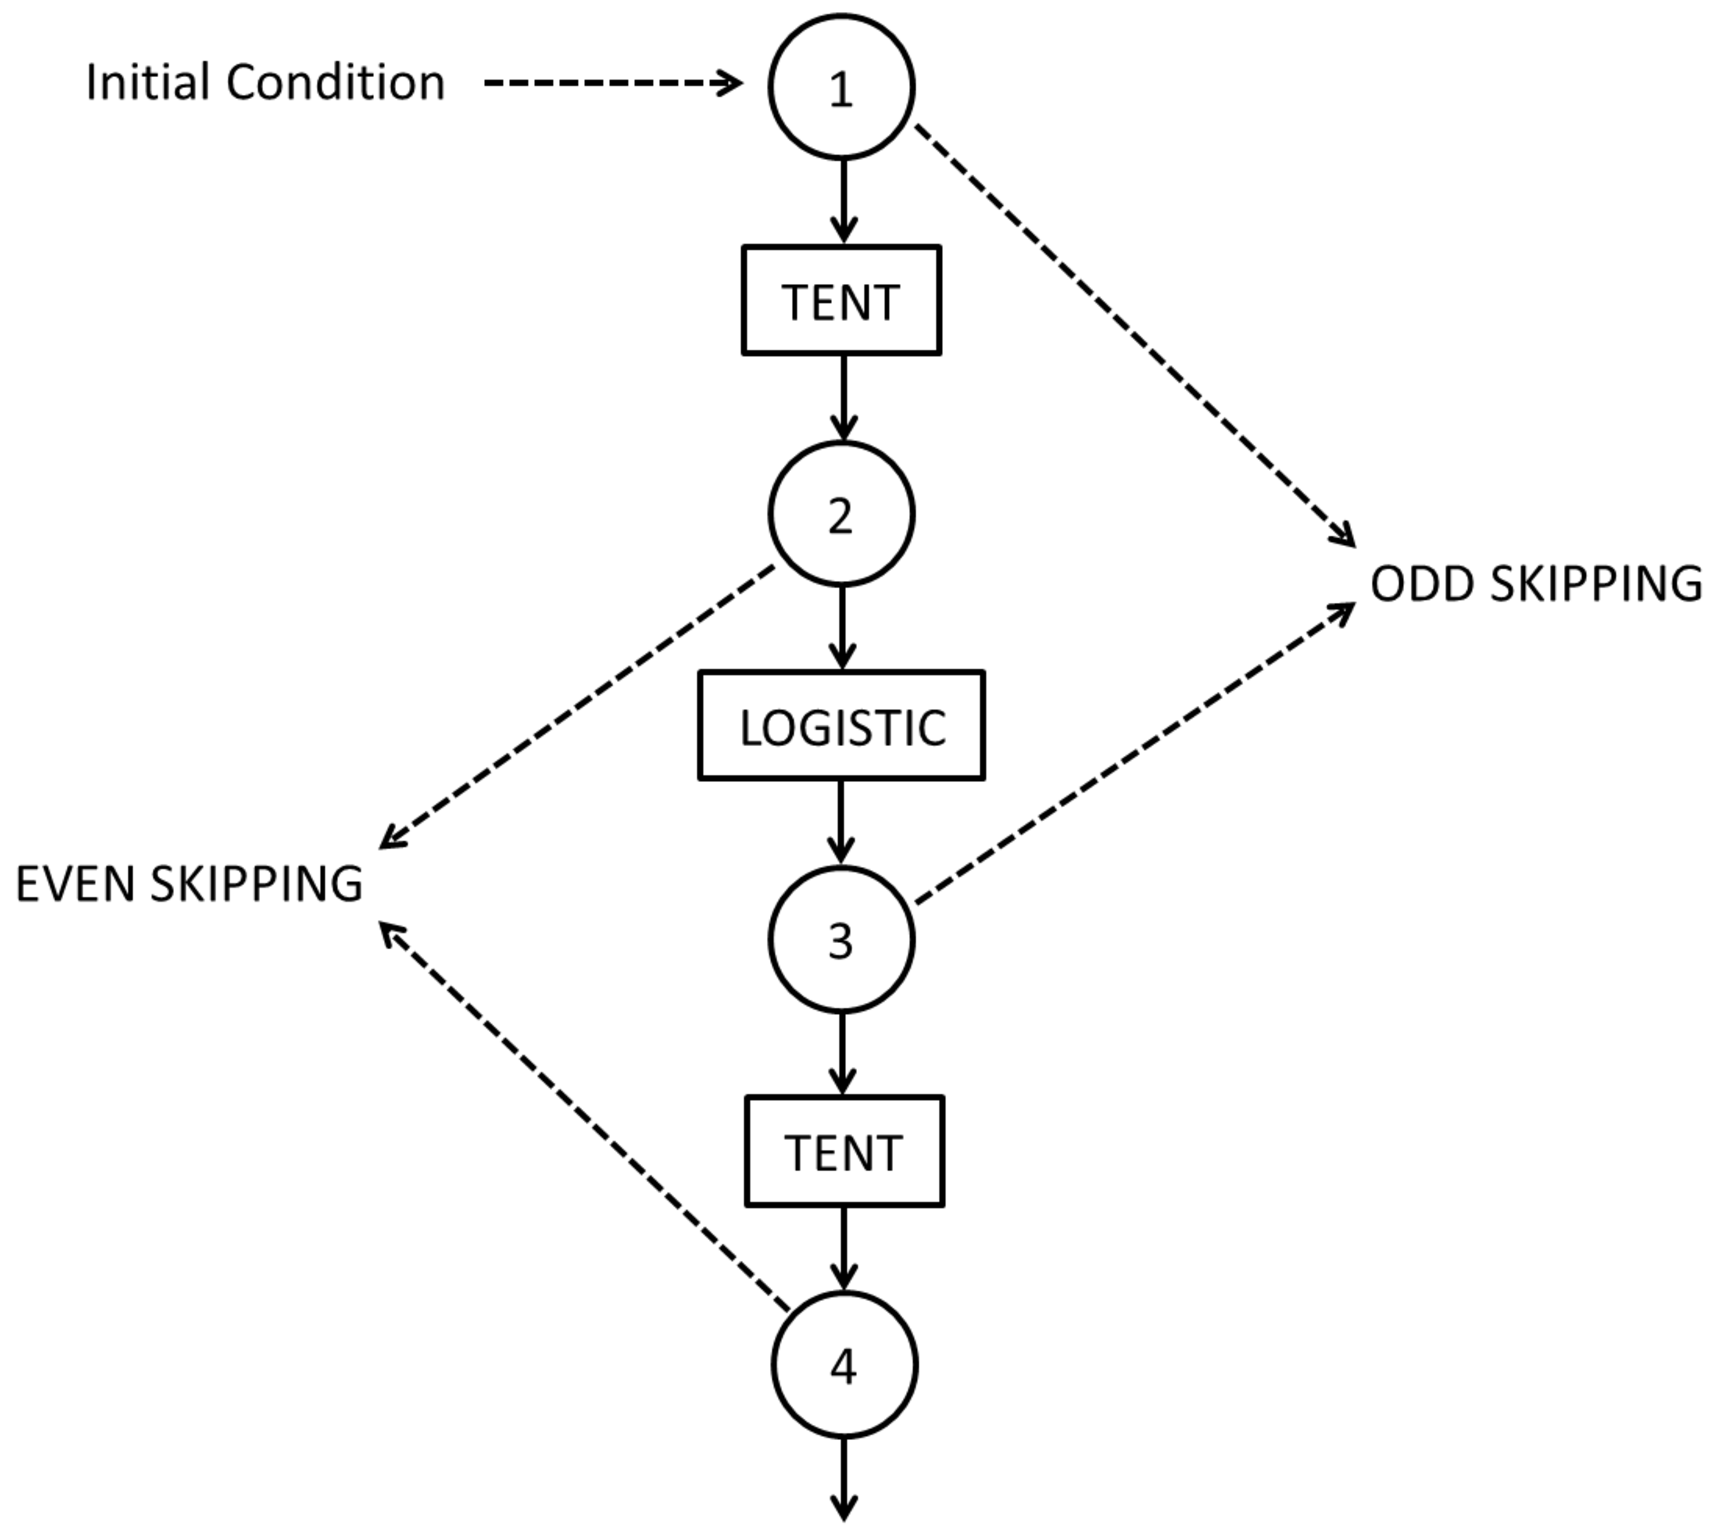
\includegraphics[height=0.4\textheight]{SwitchParImpar}
\caption{ZONA CH REHACER} \label{fig:plane zone}
\end{figure}
%%%%%%%%%%%%%%%%%%%%%%%%%%
%%%%%%%%%%%%%%%%%%%%%%%%%%% Fig.1
%
\begin{figure}
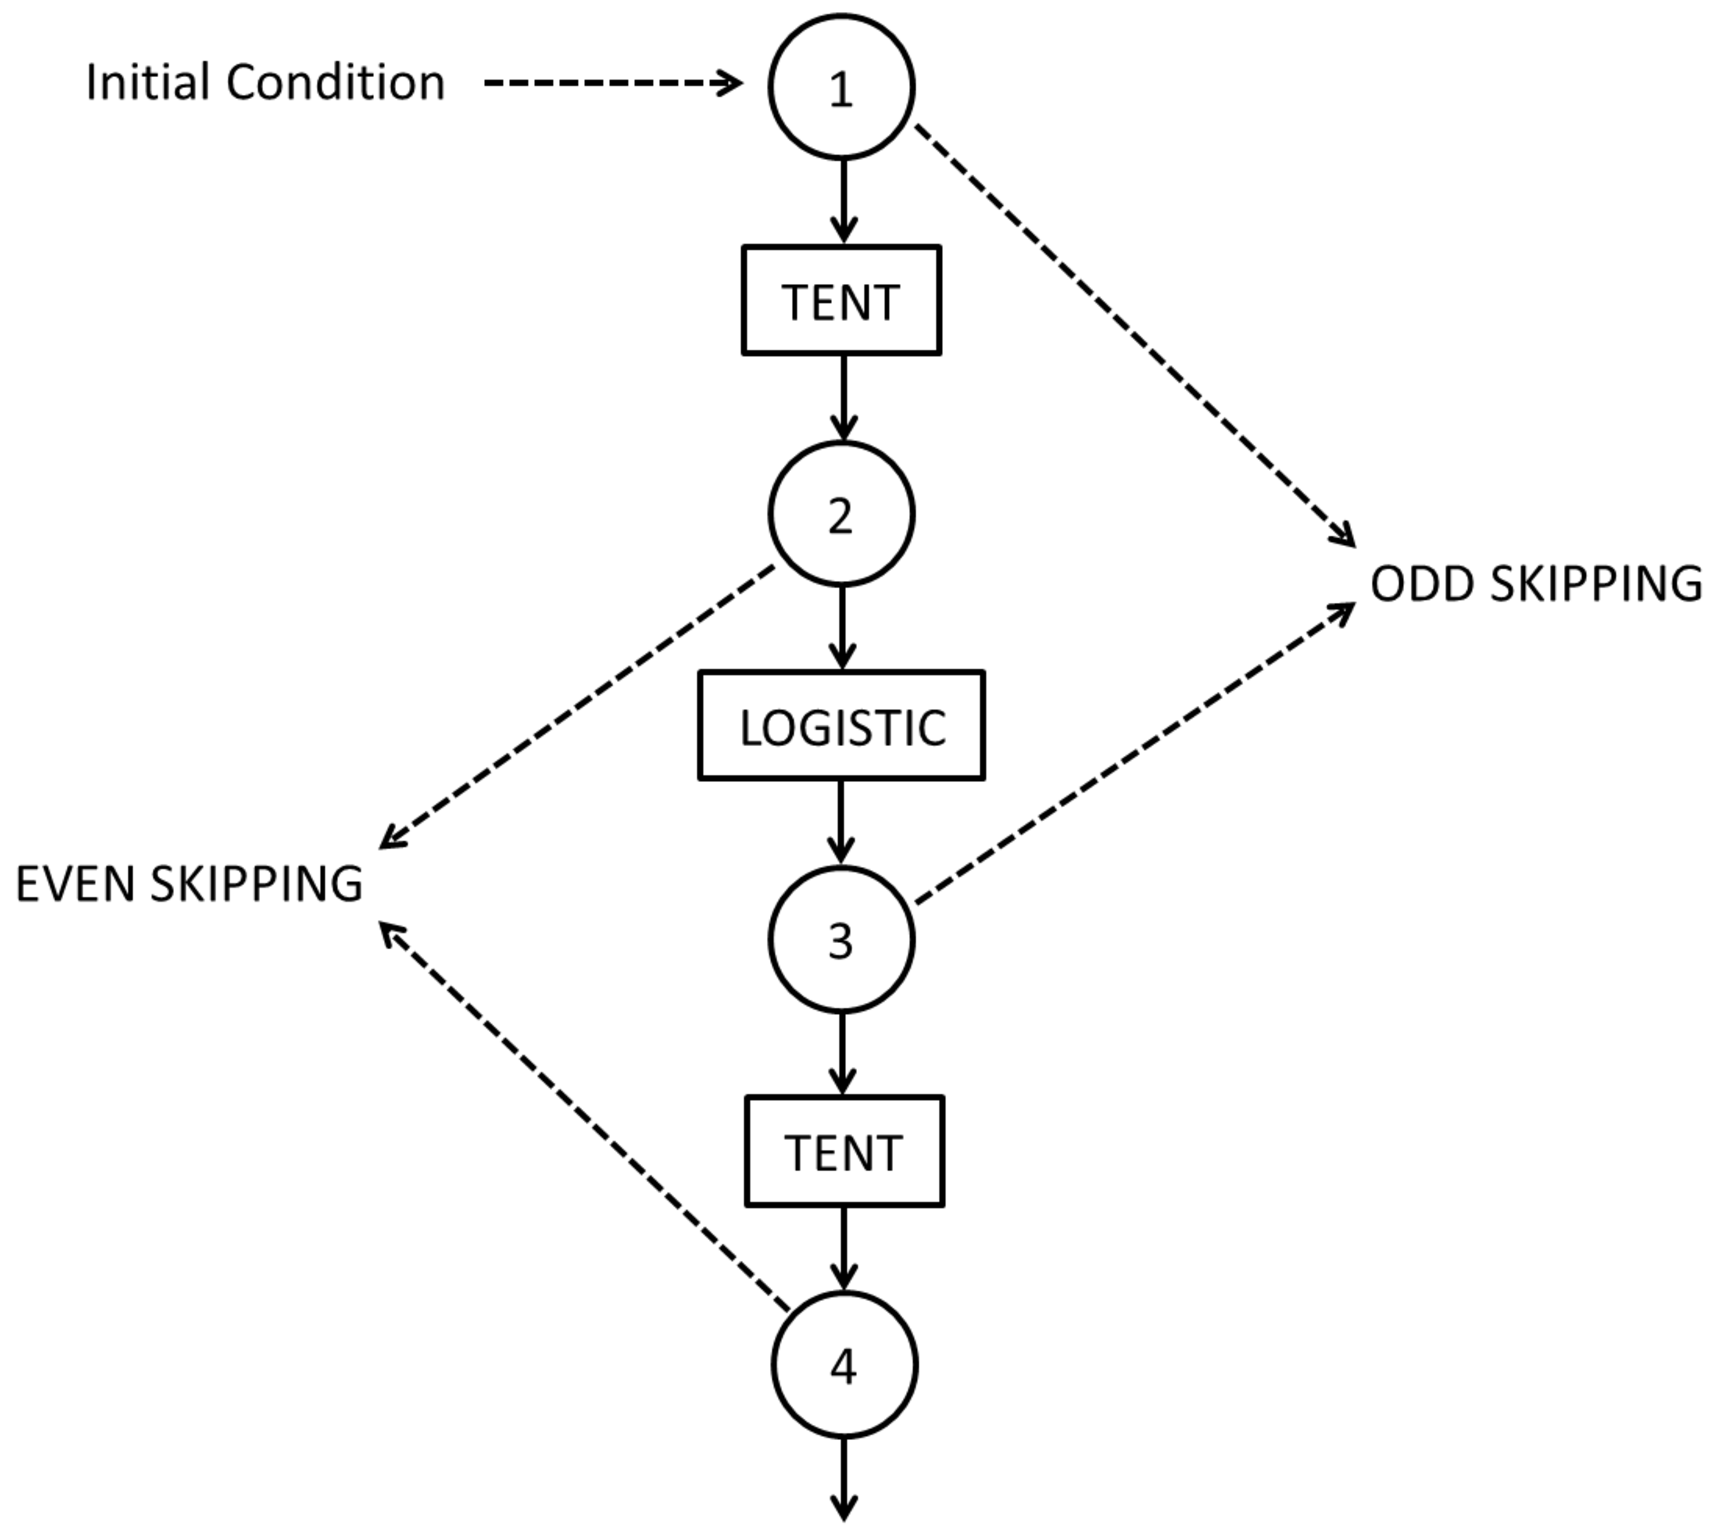
\includegraphics[height=0.4\textheight]{SwitchParImpar}
\caption{Sequential switching between Tent and Logistic maps. In the figure are also shown even and odd skipping strategies} \label{fig:seq}
\end{figure}
%%%%%%%%%%%%%%%%%%%%%%%%%%
%%%%%%%%%%%%%%%%%%%%%%%%%%% Fig.2
\begin{figure}
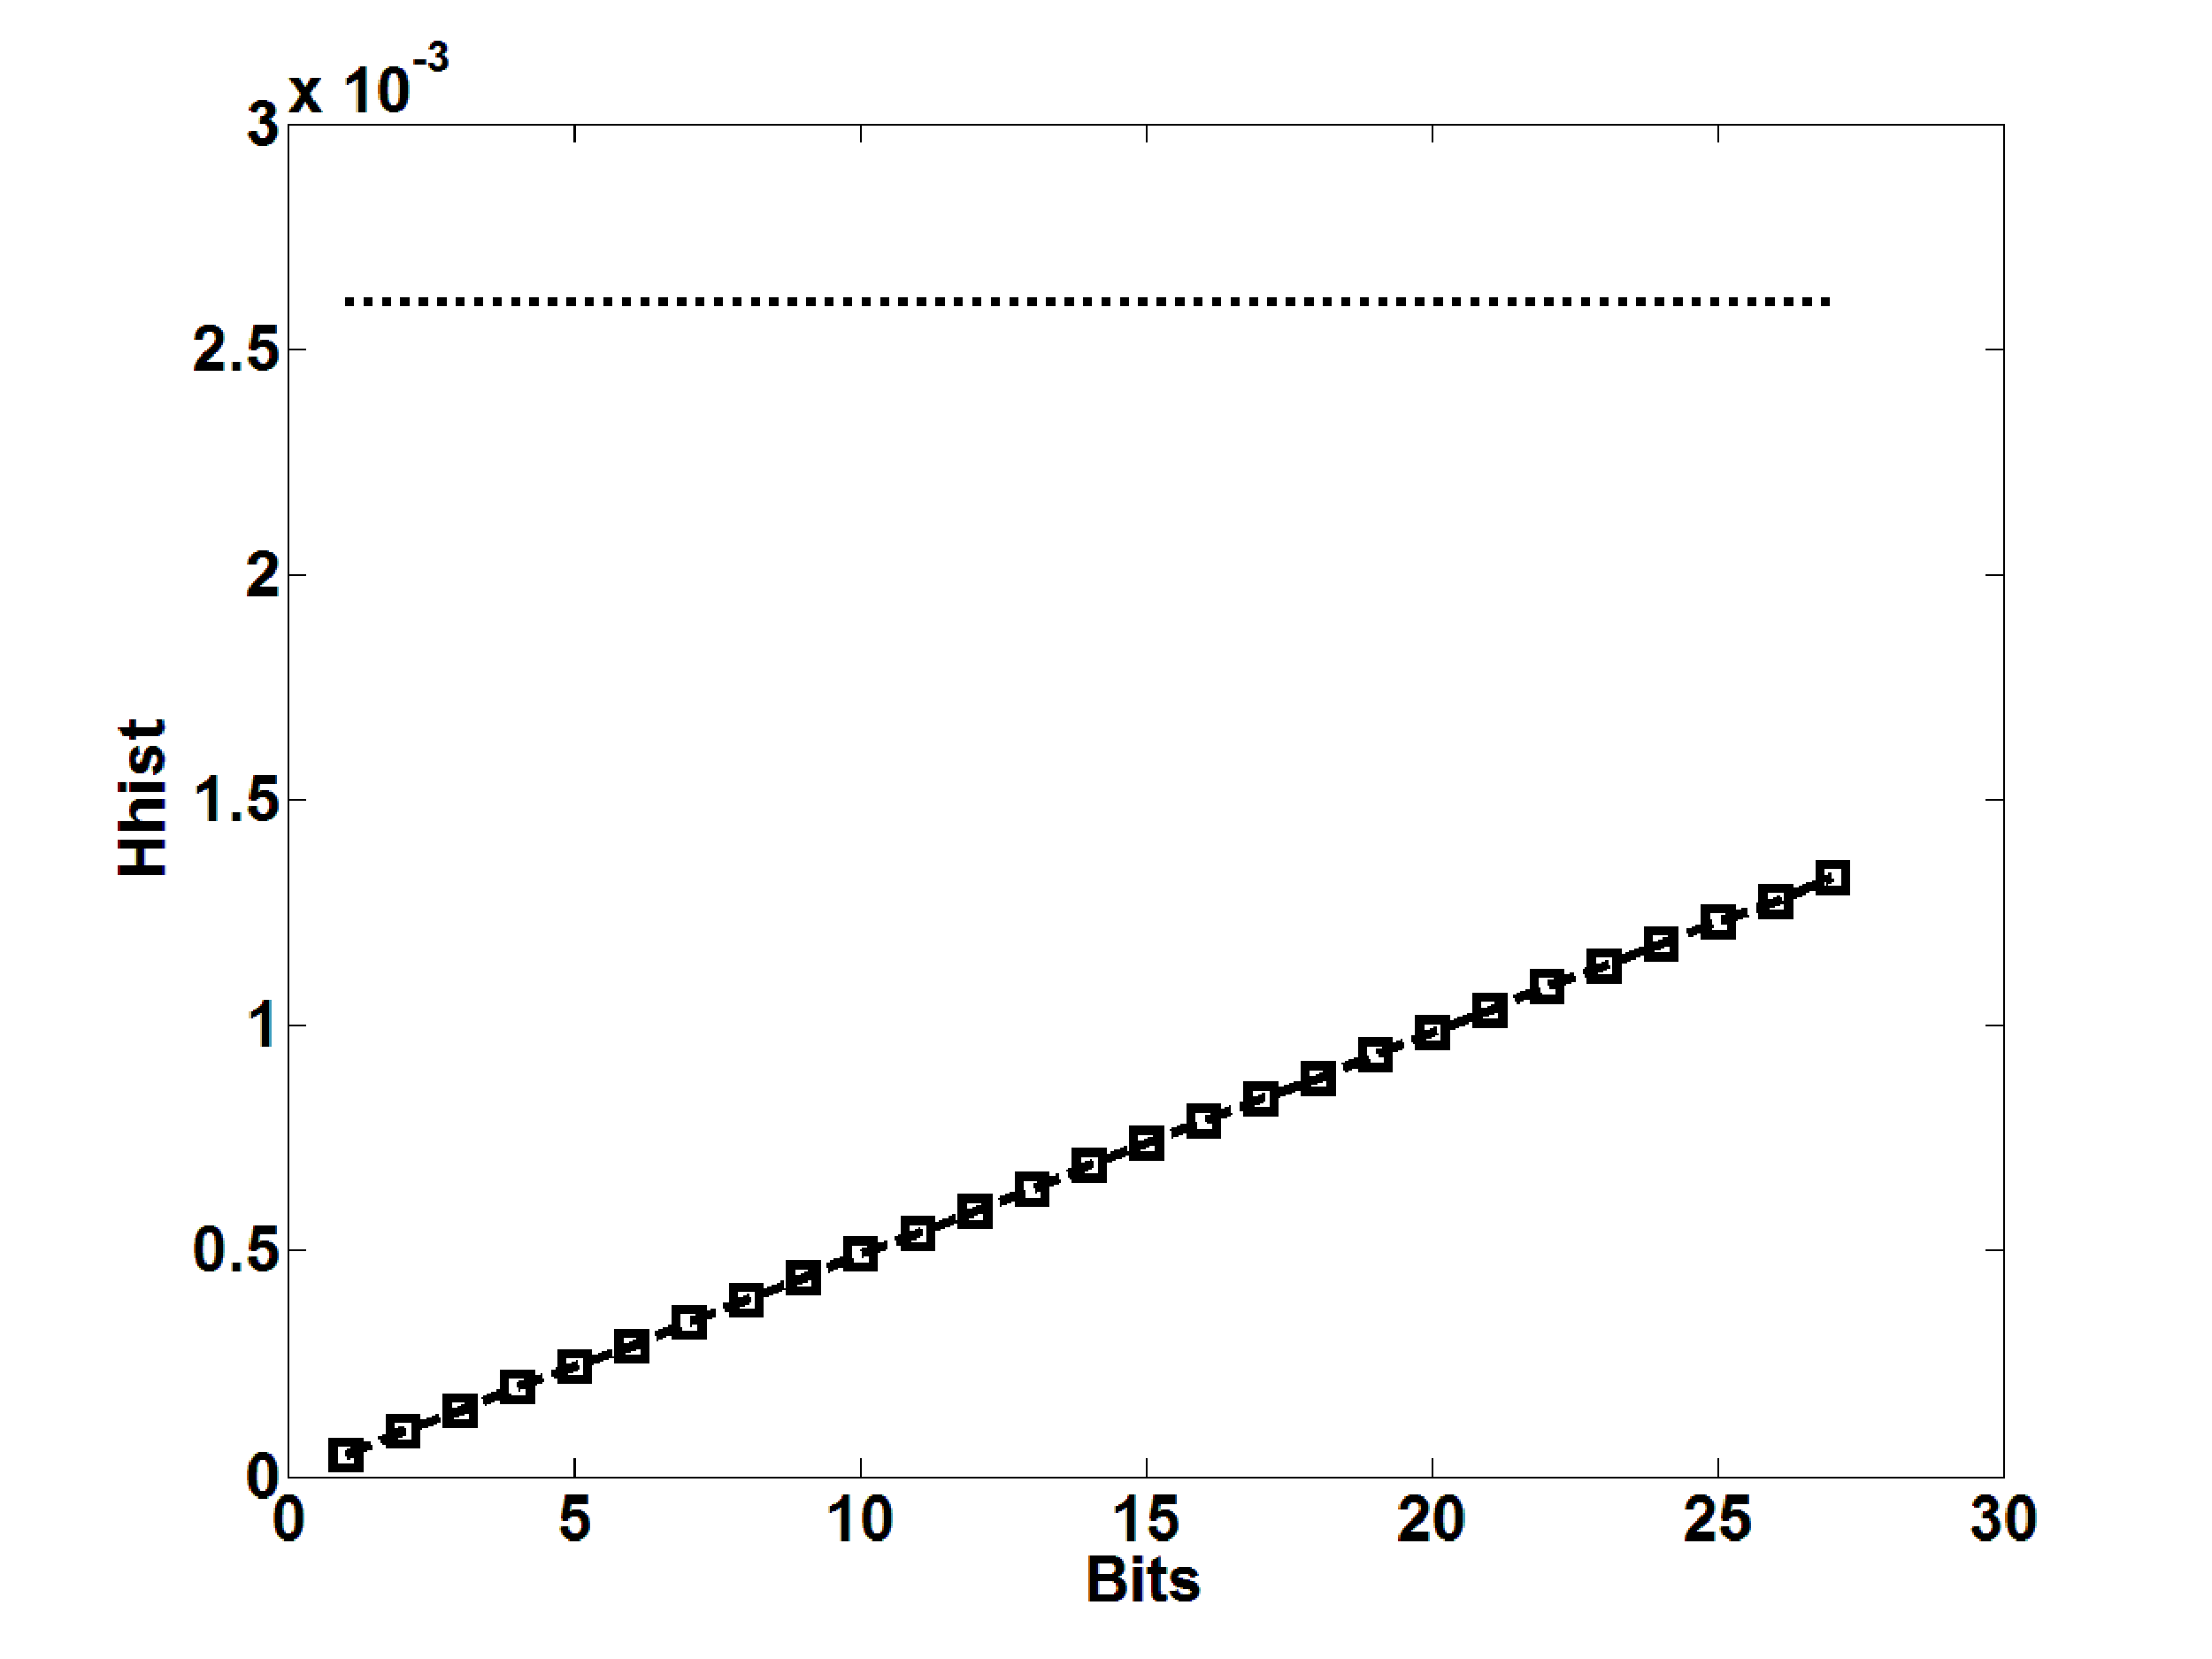
\includegraphics[width=0.3\textwidth]{Hhist_tentB10}
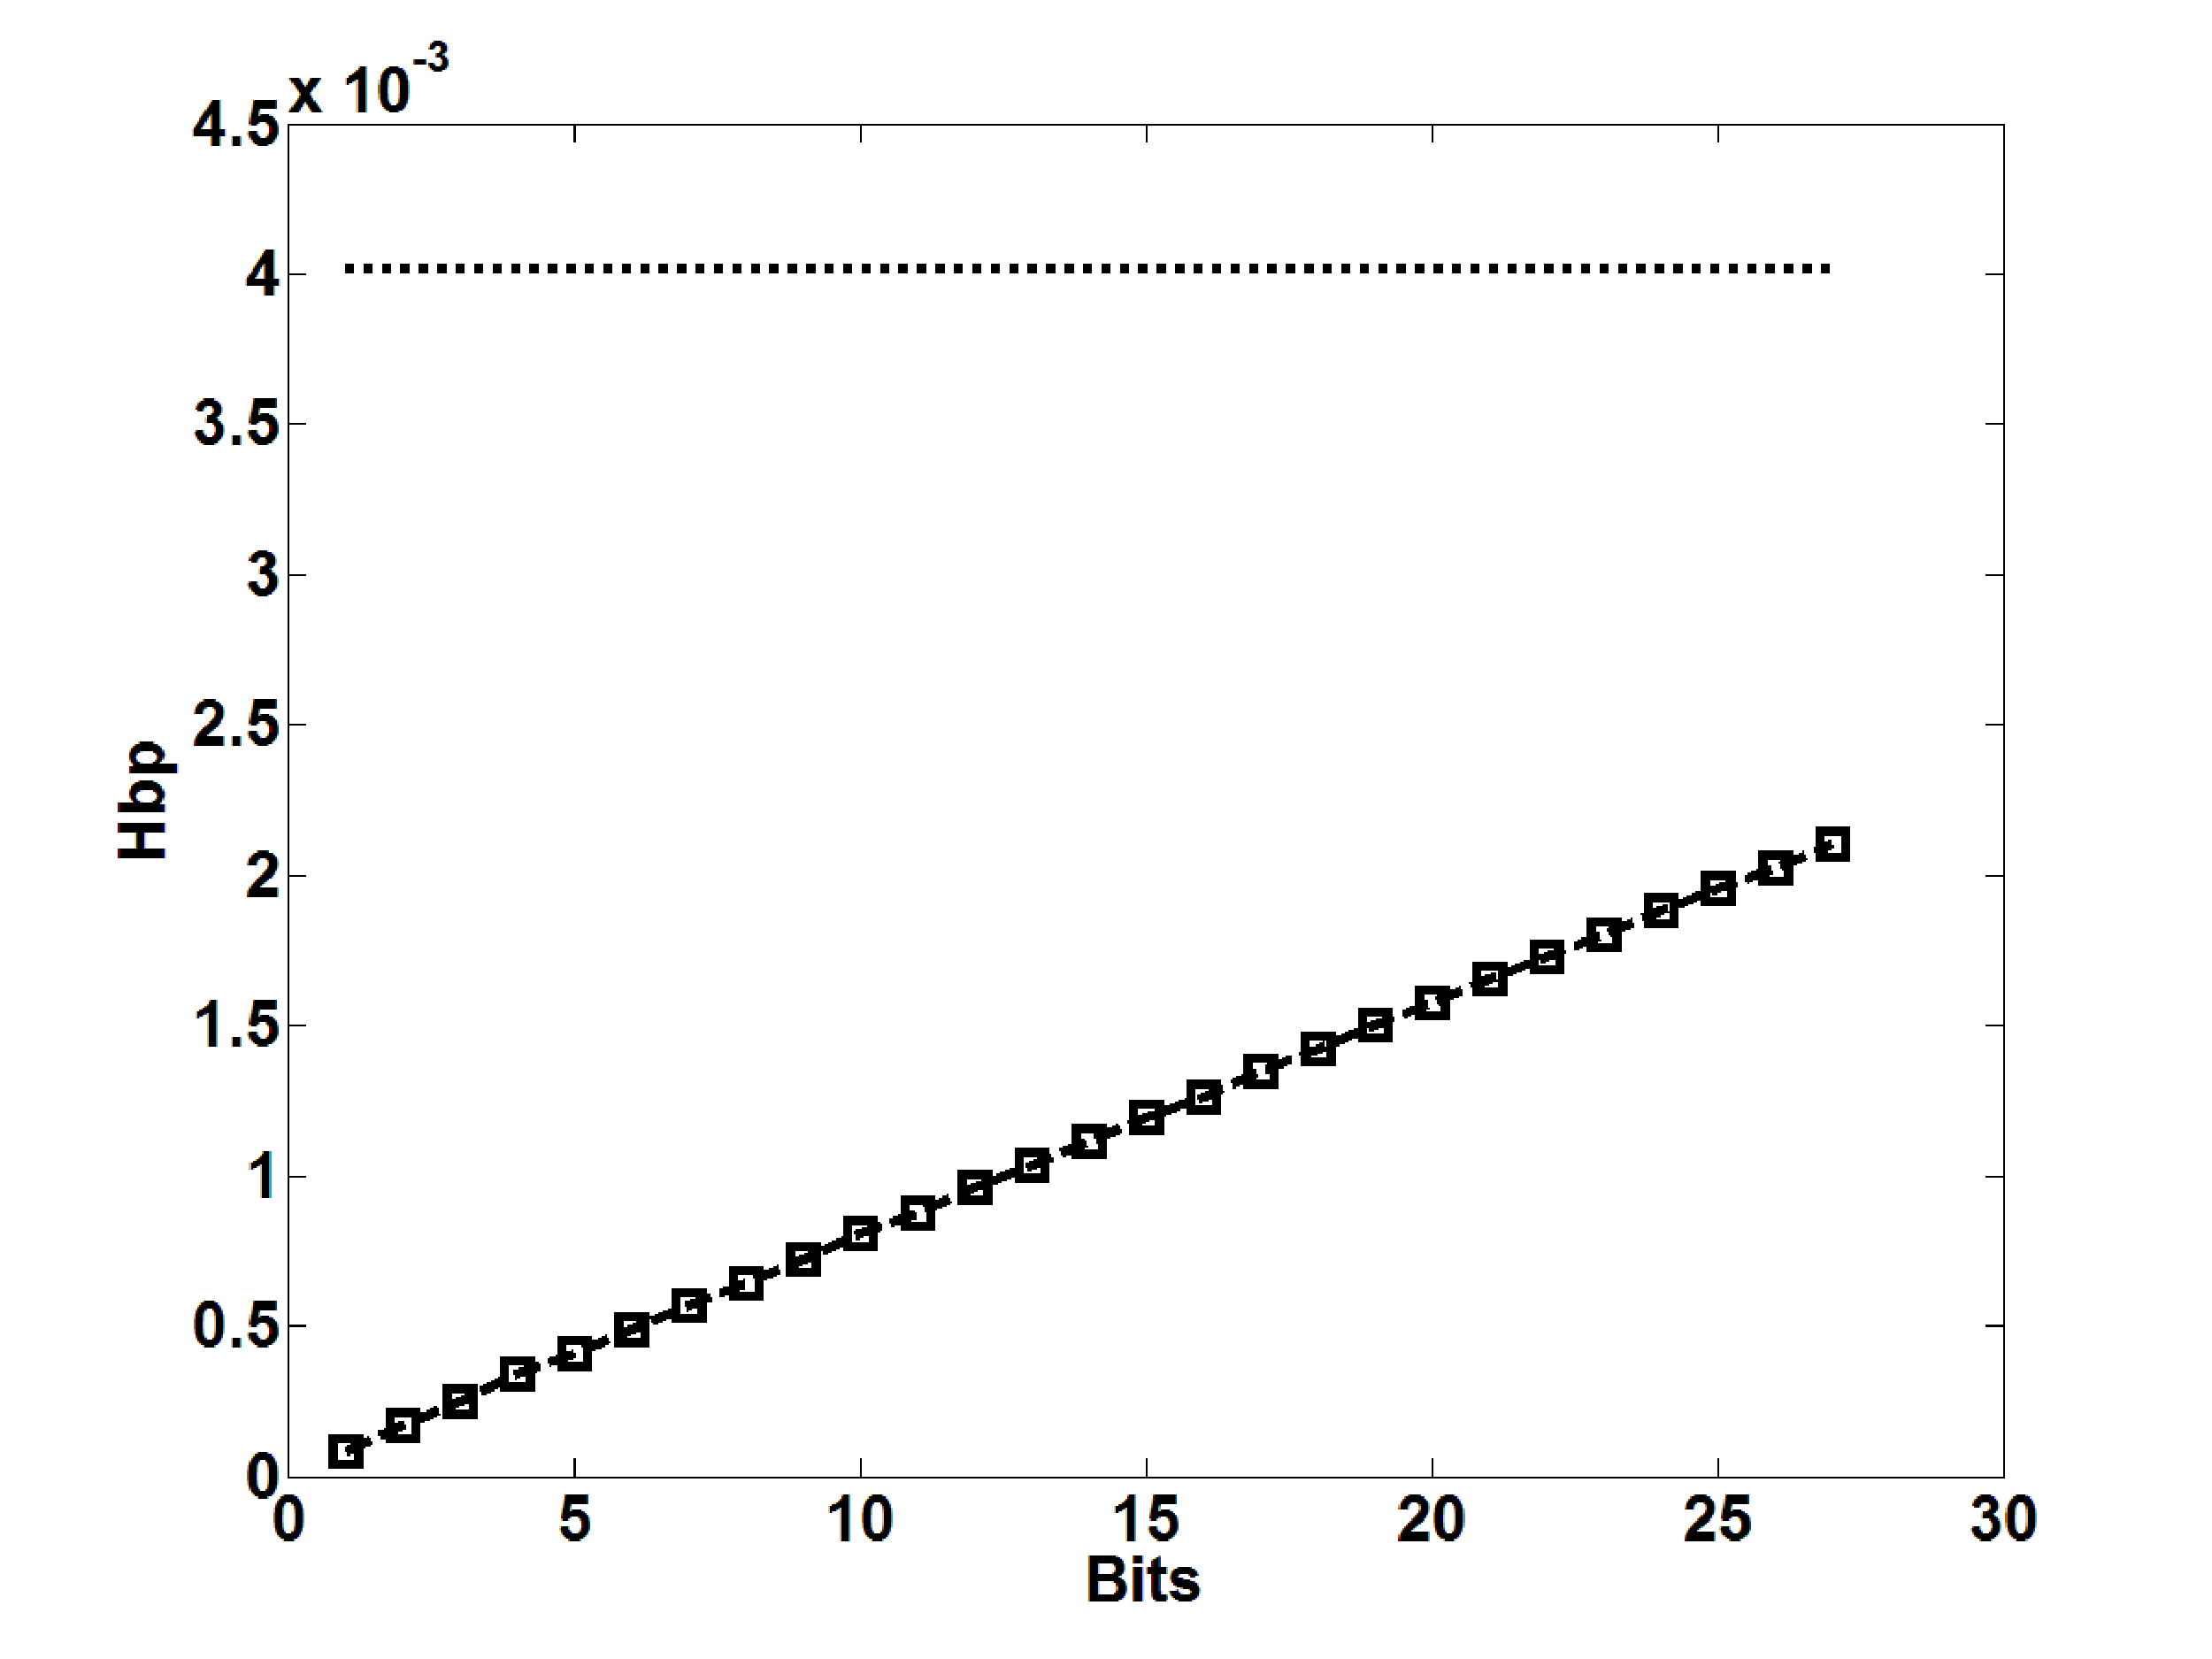
\includegraphics[width=0.3\textwidth]{Hbp_tentB10}
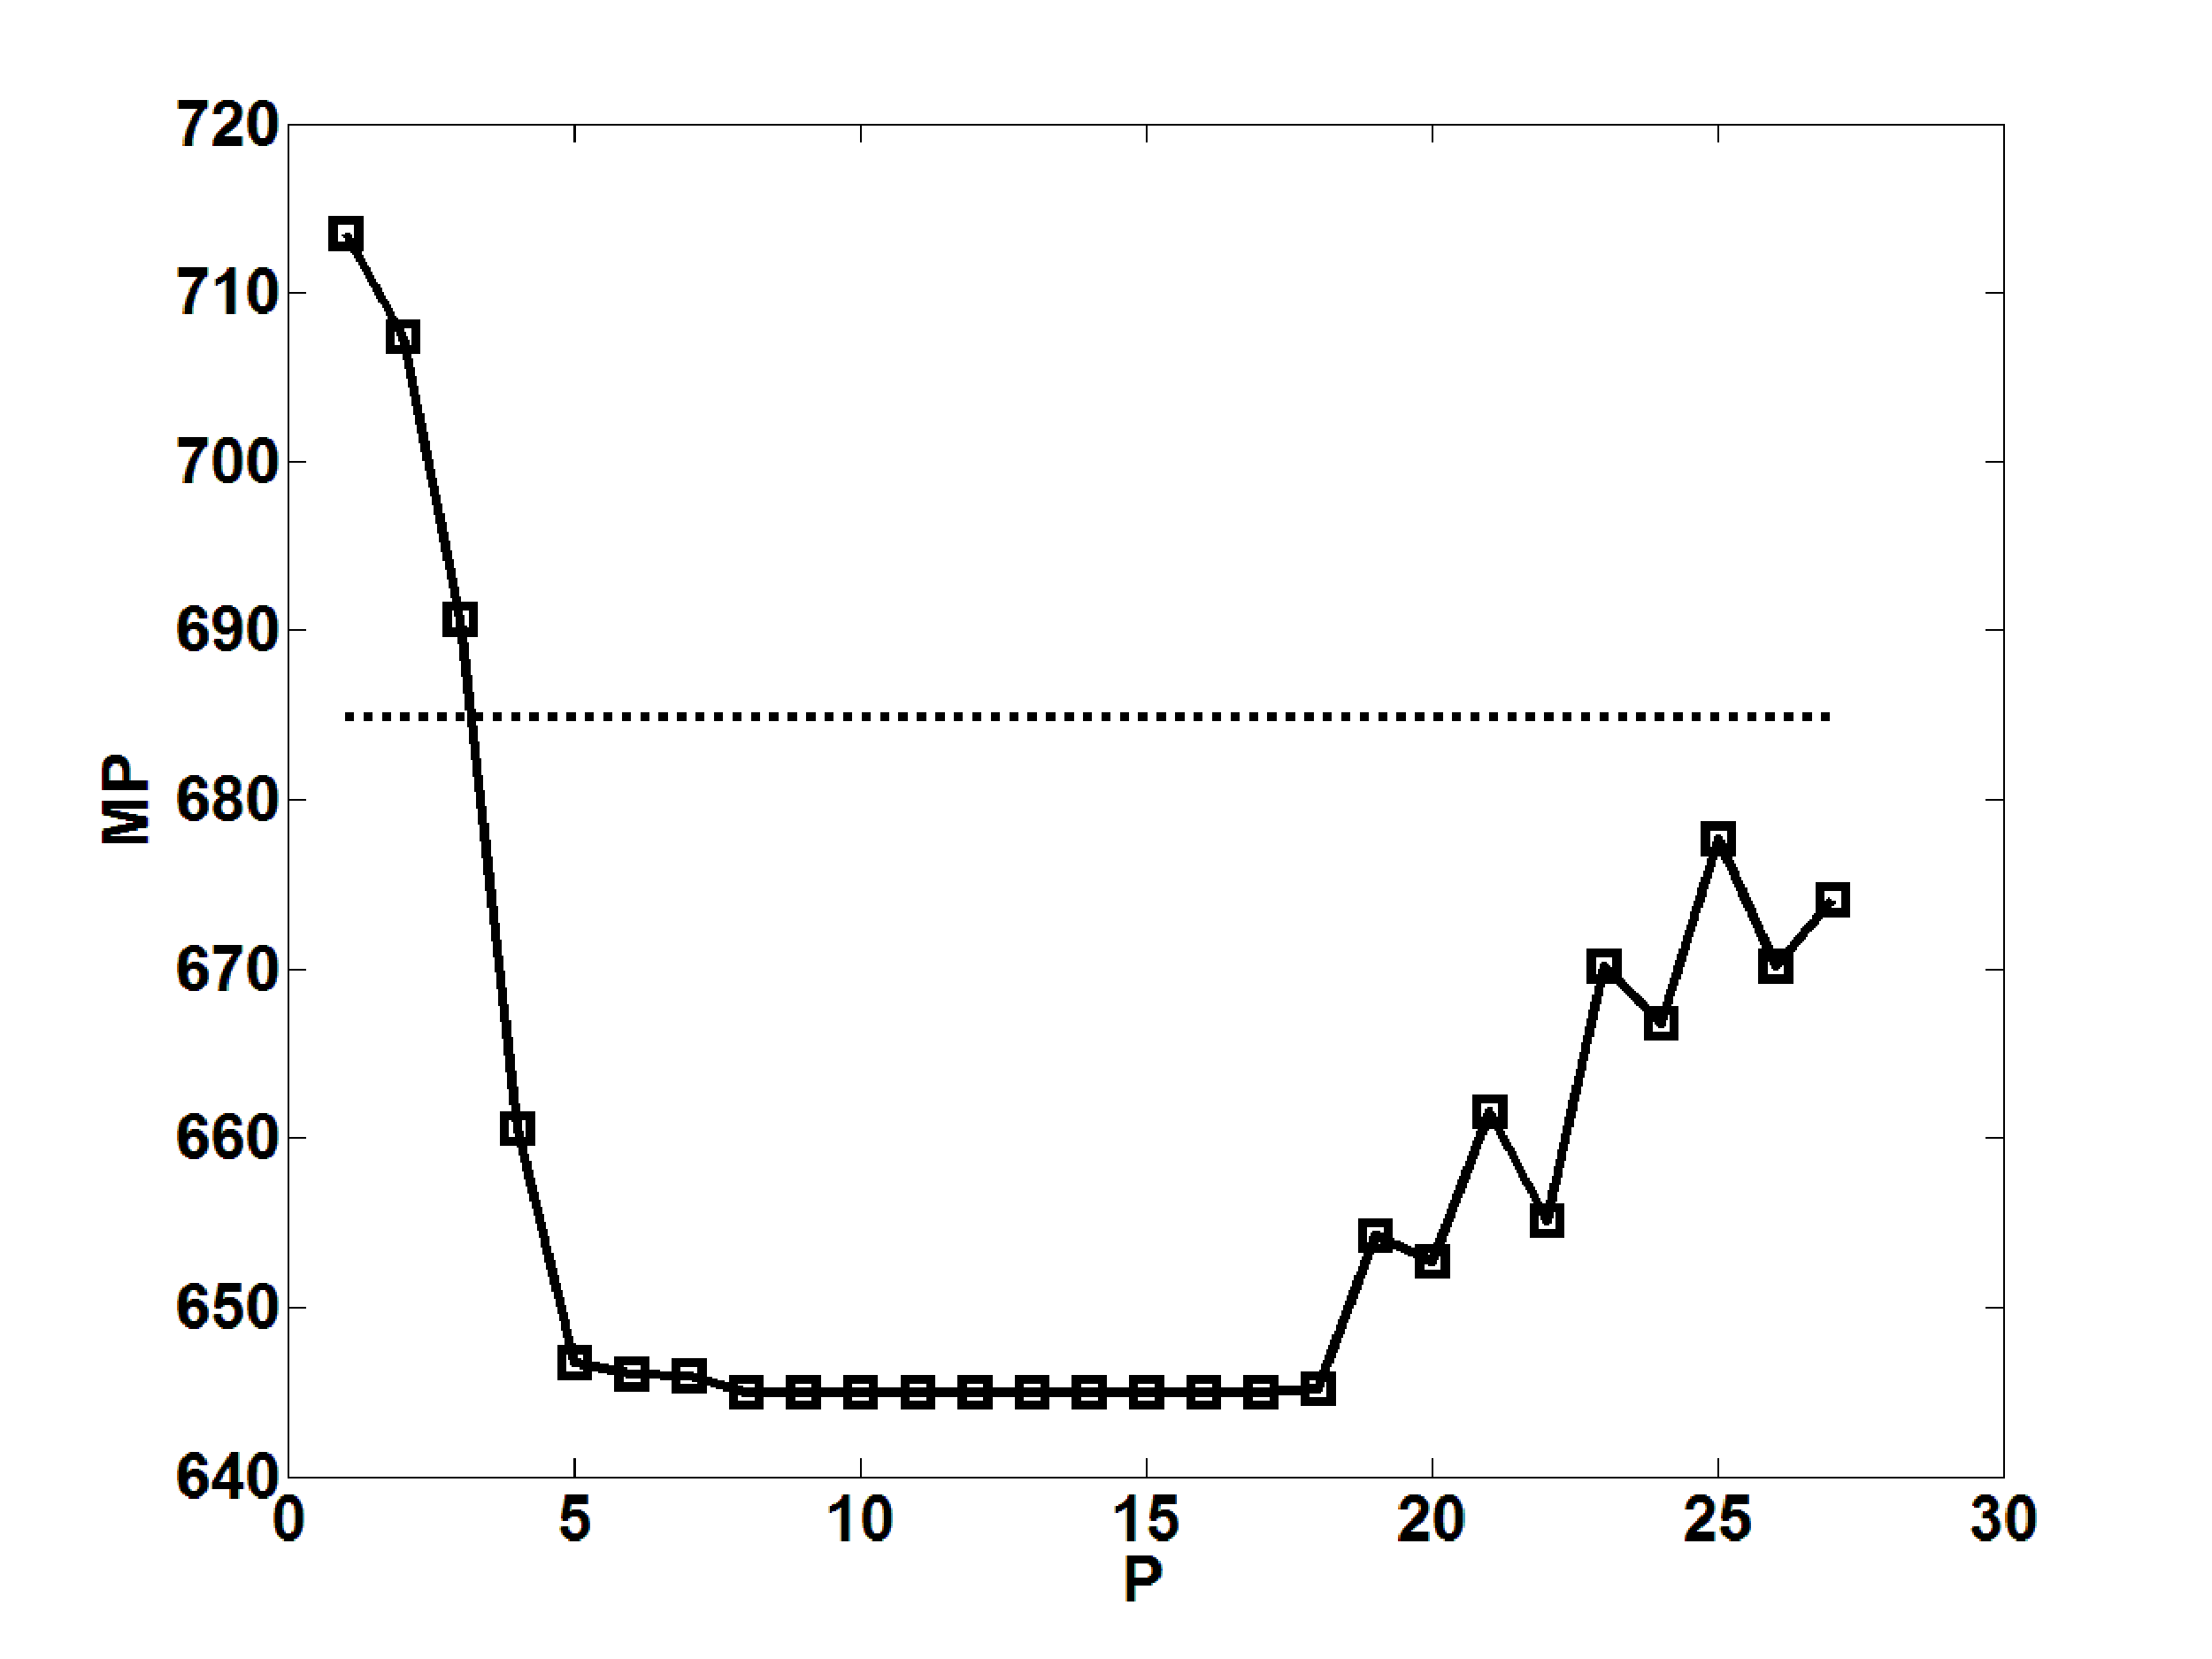
\includegraphics[width=0.3\textwidth]{Miss_tentB10}
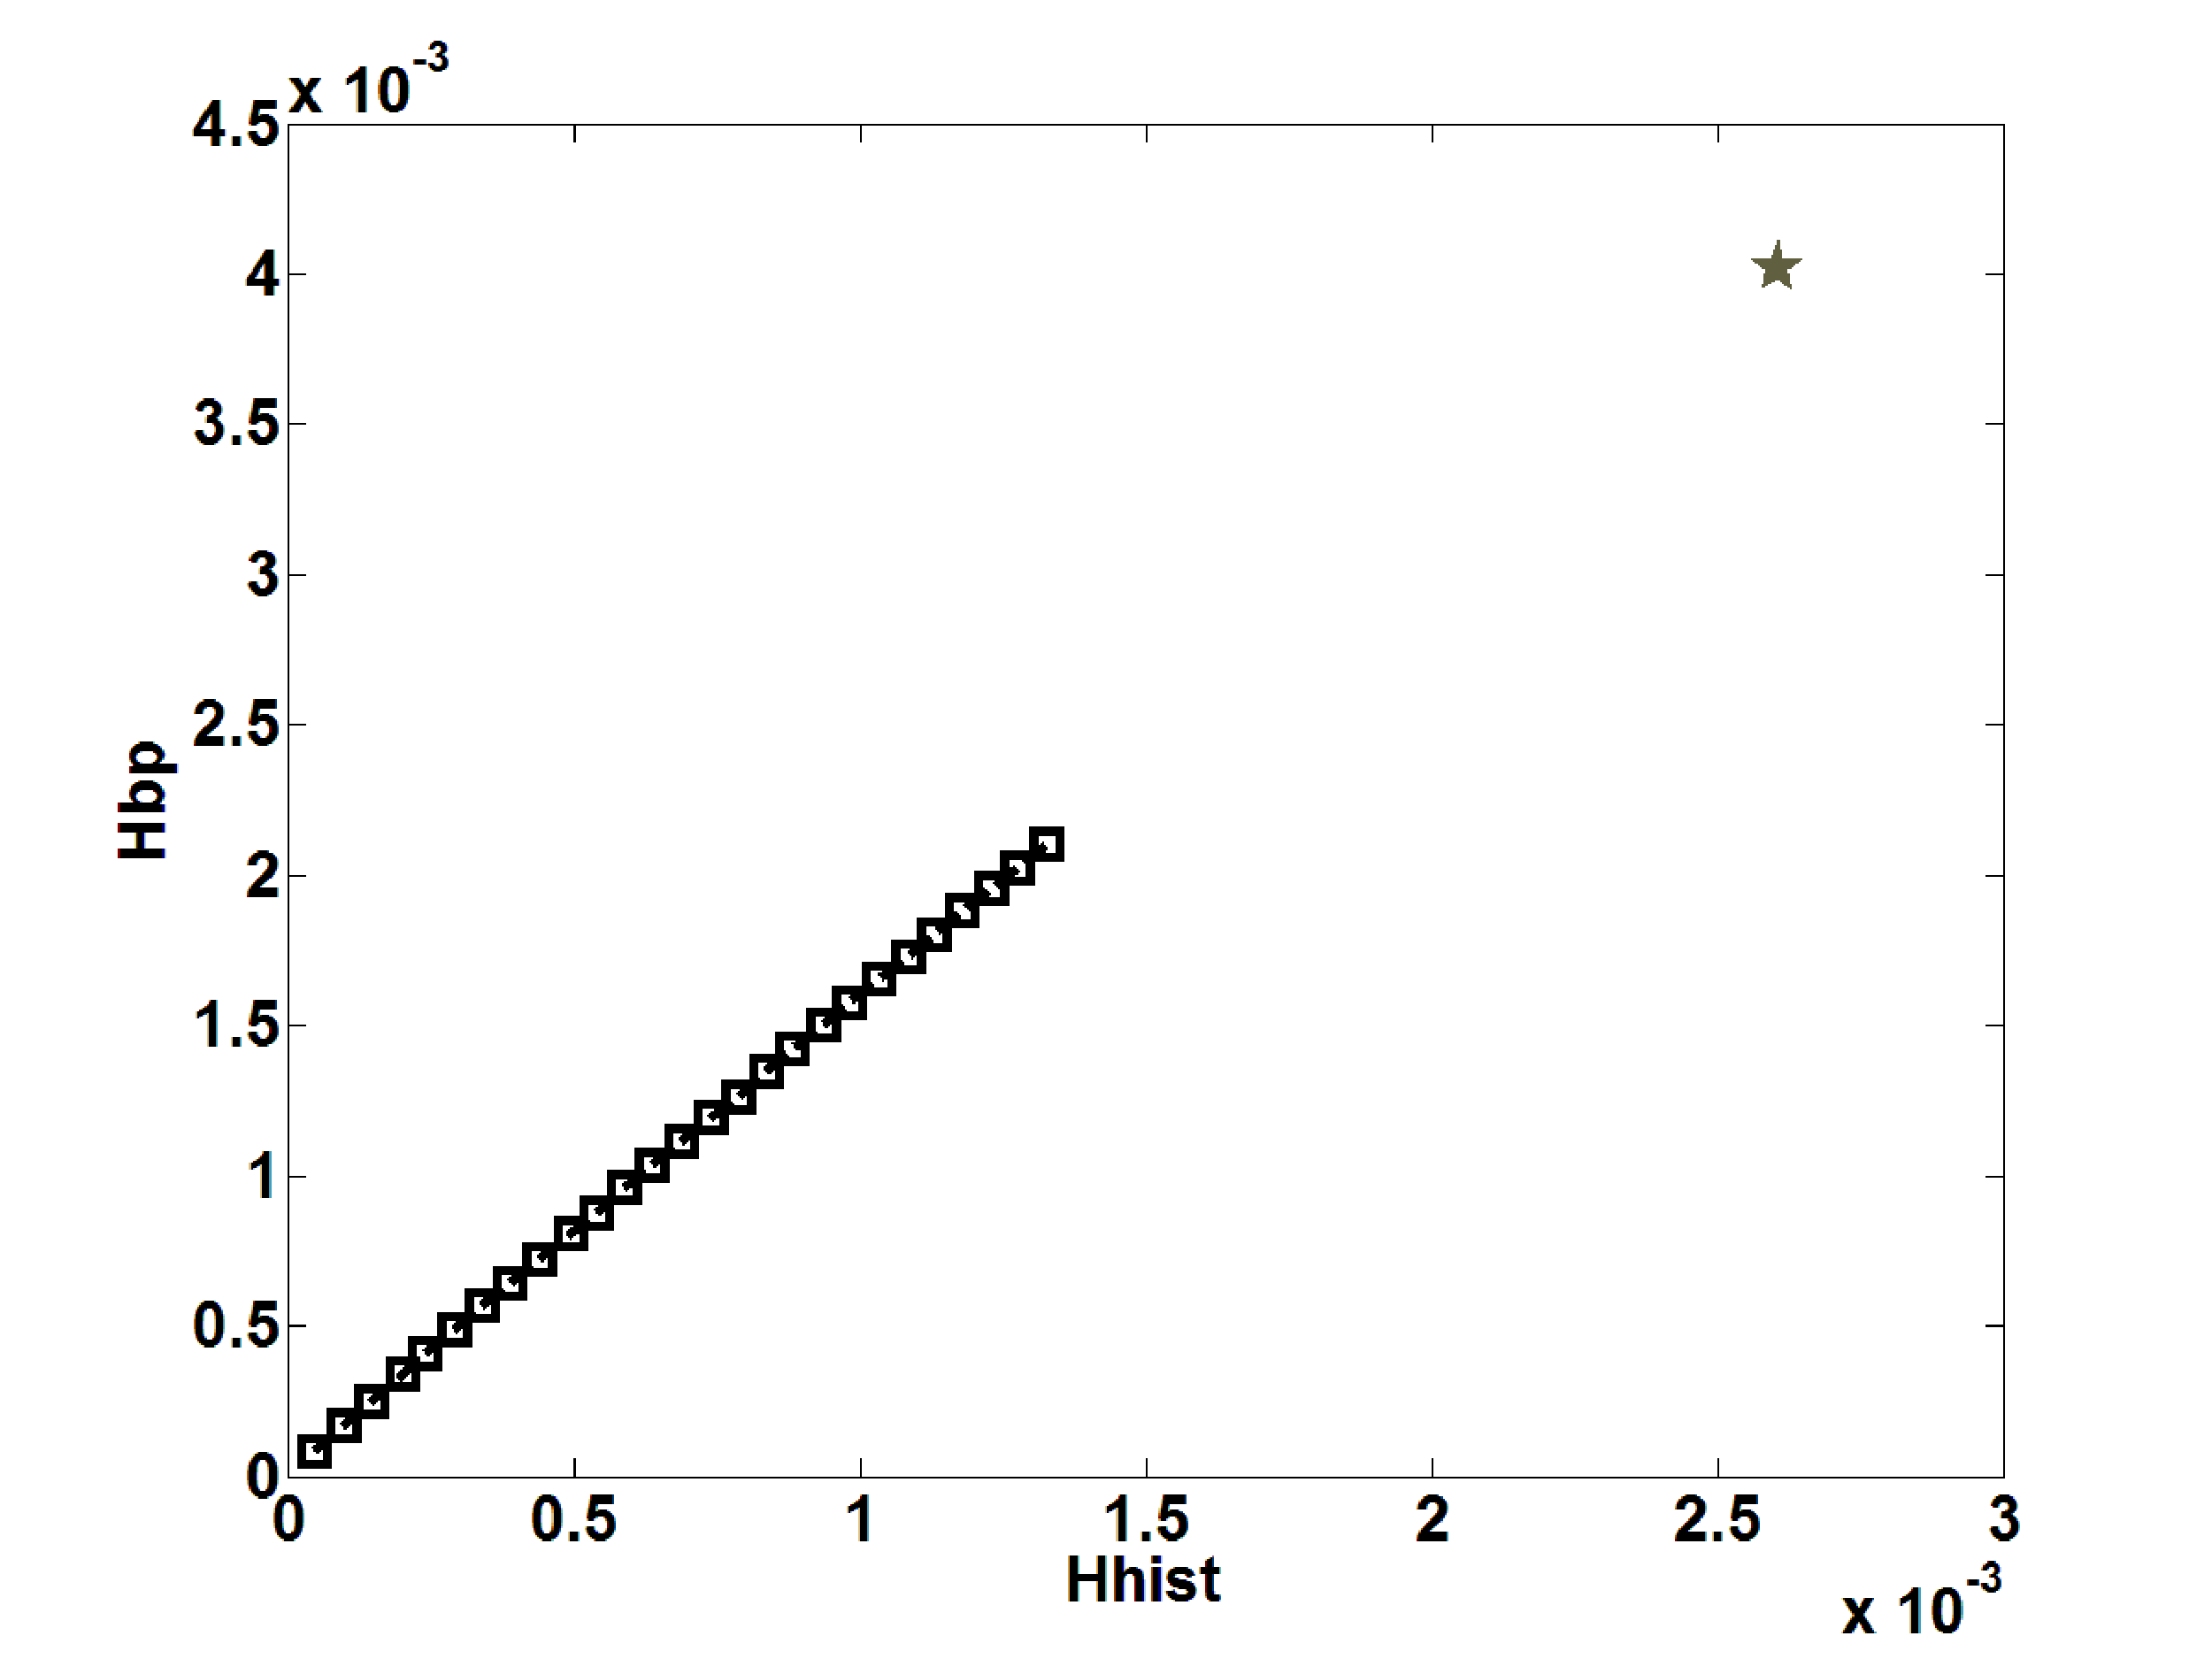
\includegraphics[width=0.3\textwidth]{HhistHbp_tentB10}
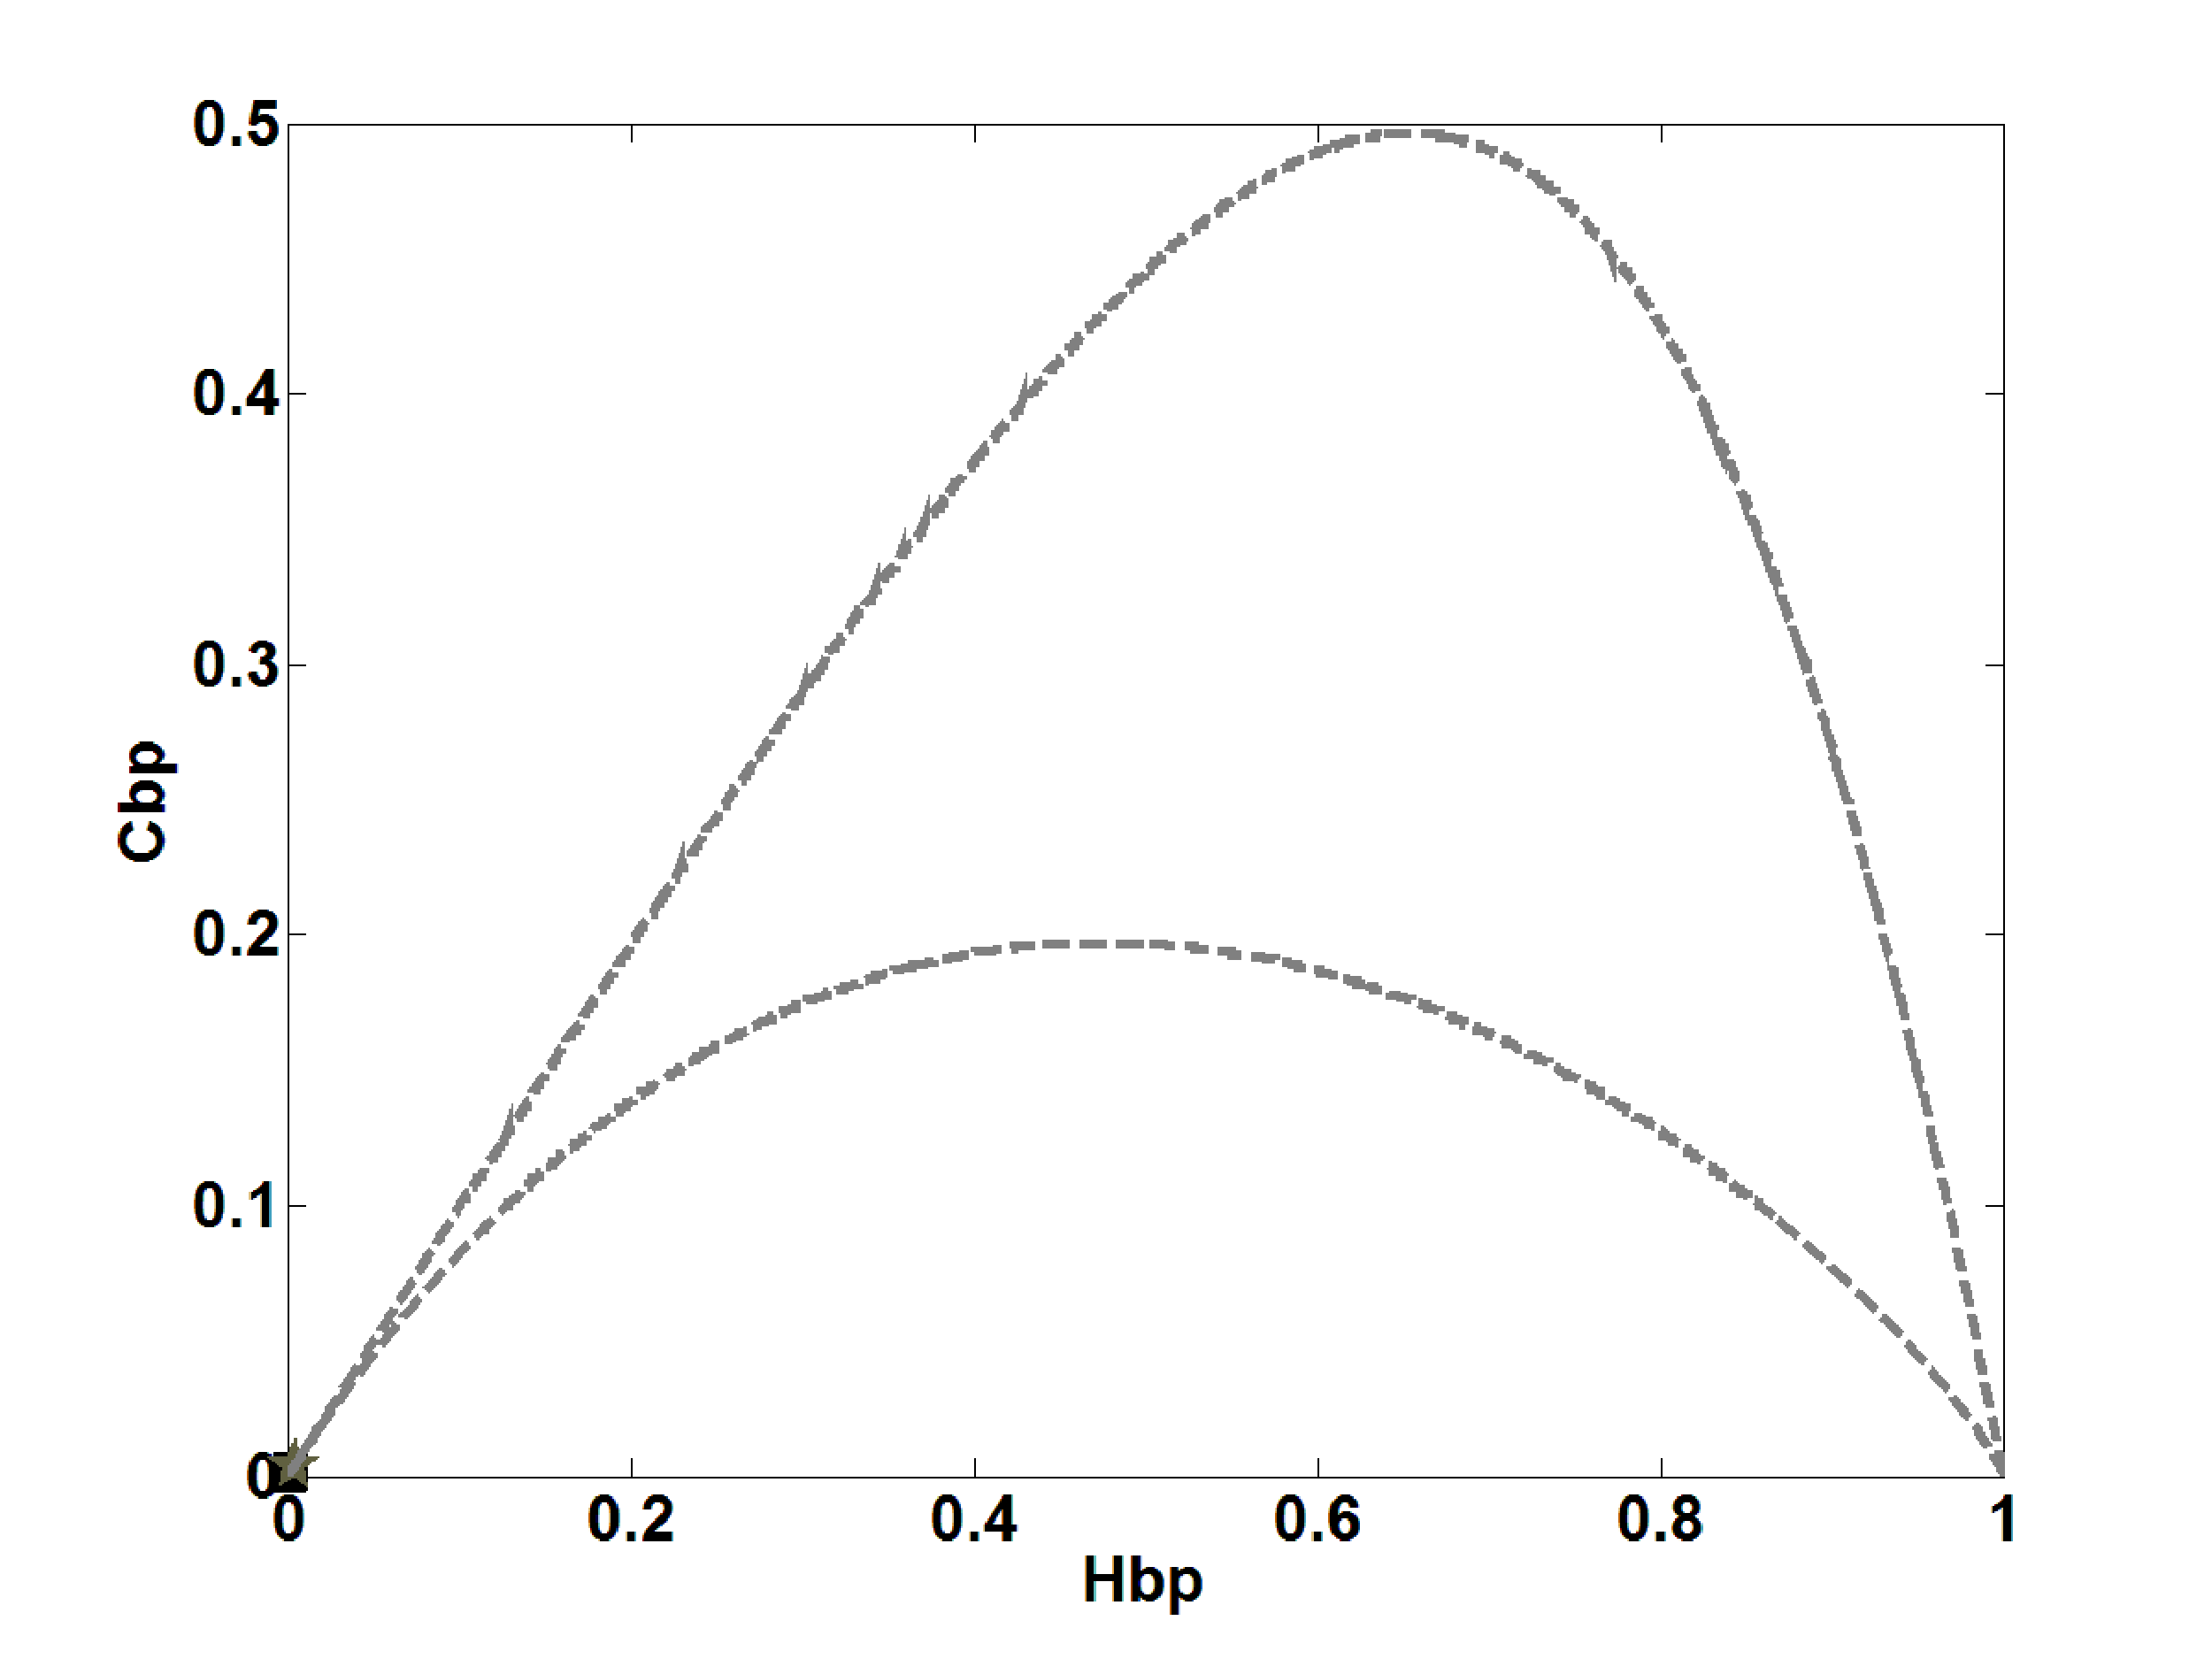
\includegraphics[width=0.3\textwidth]{HbpCbp_tentB10}
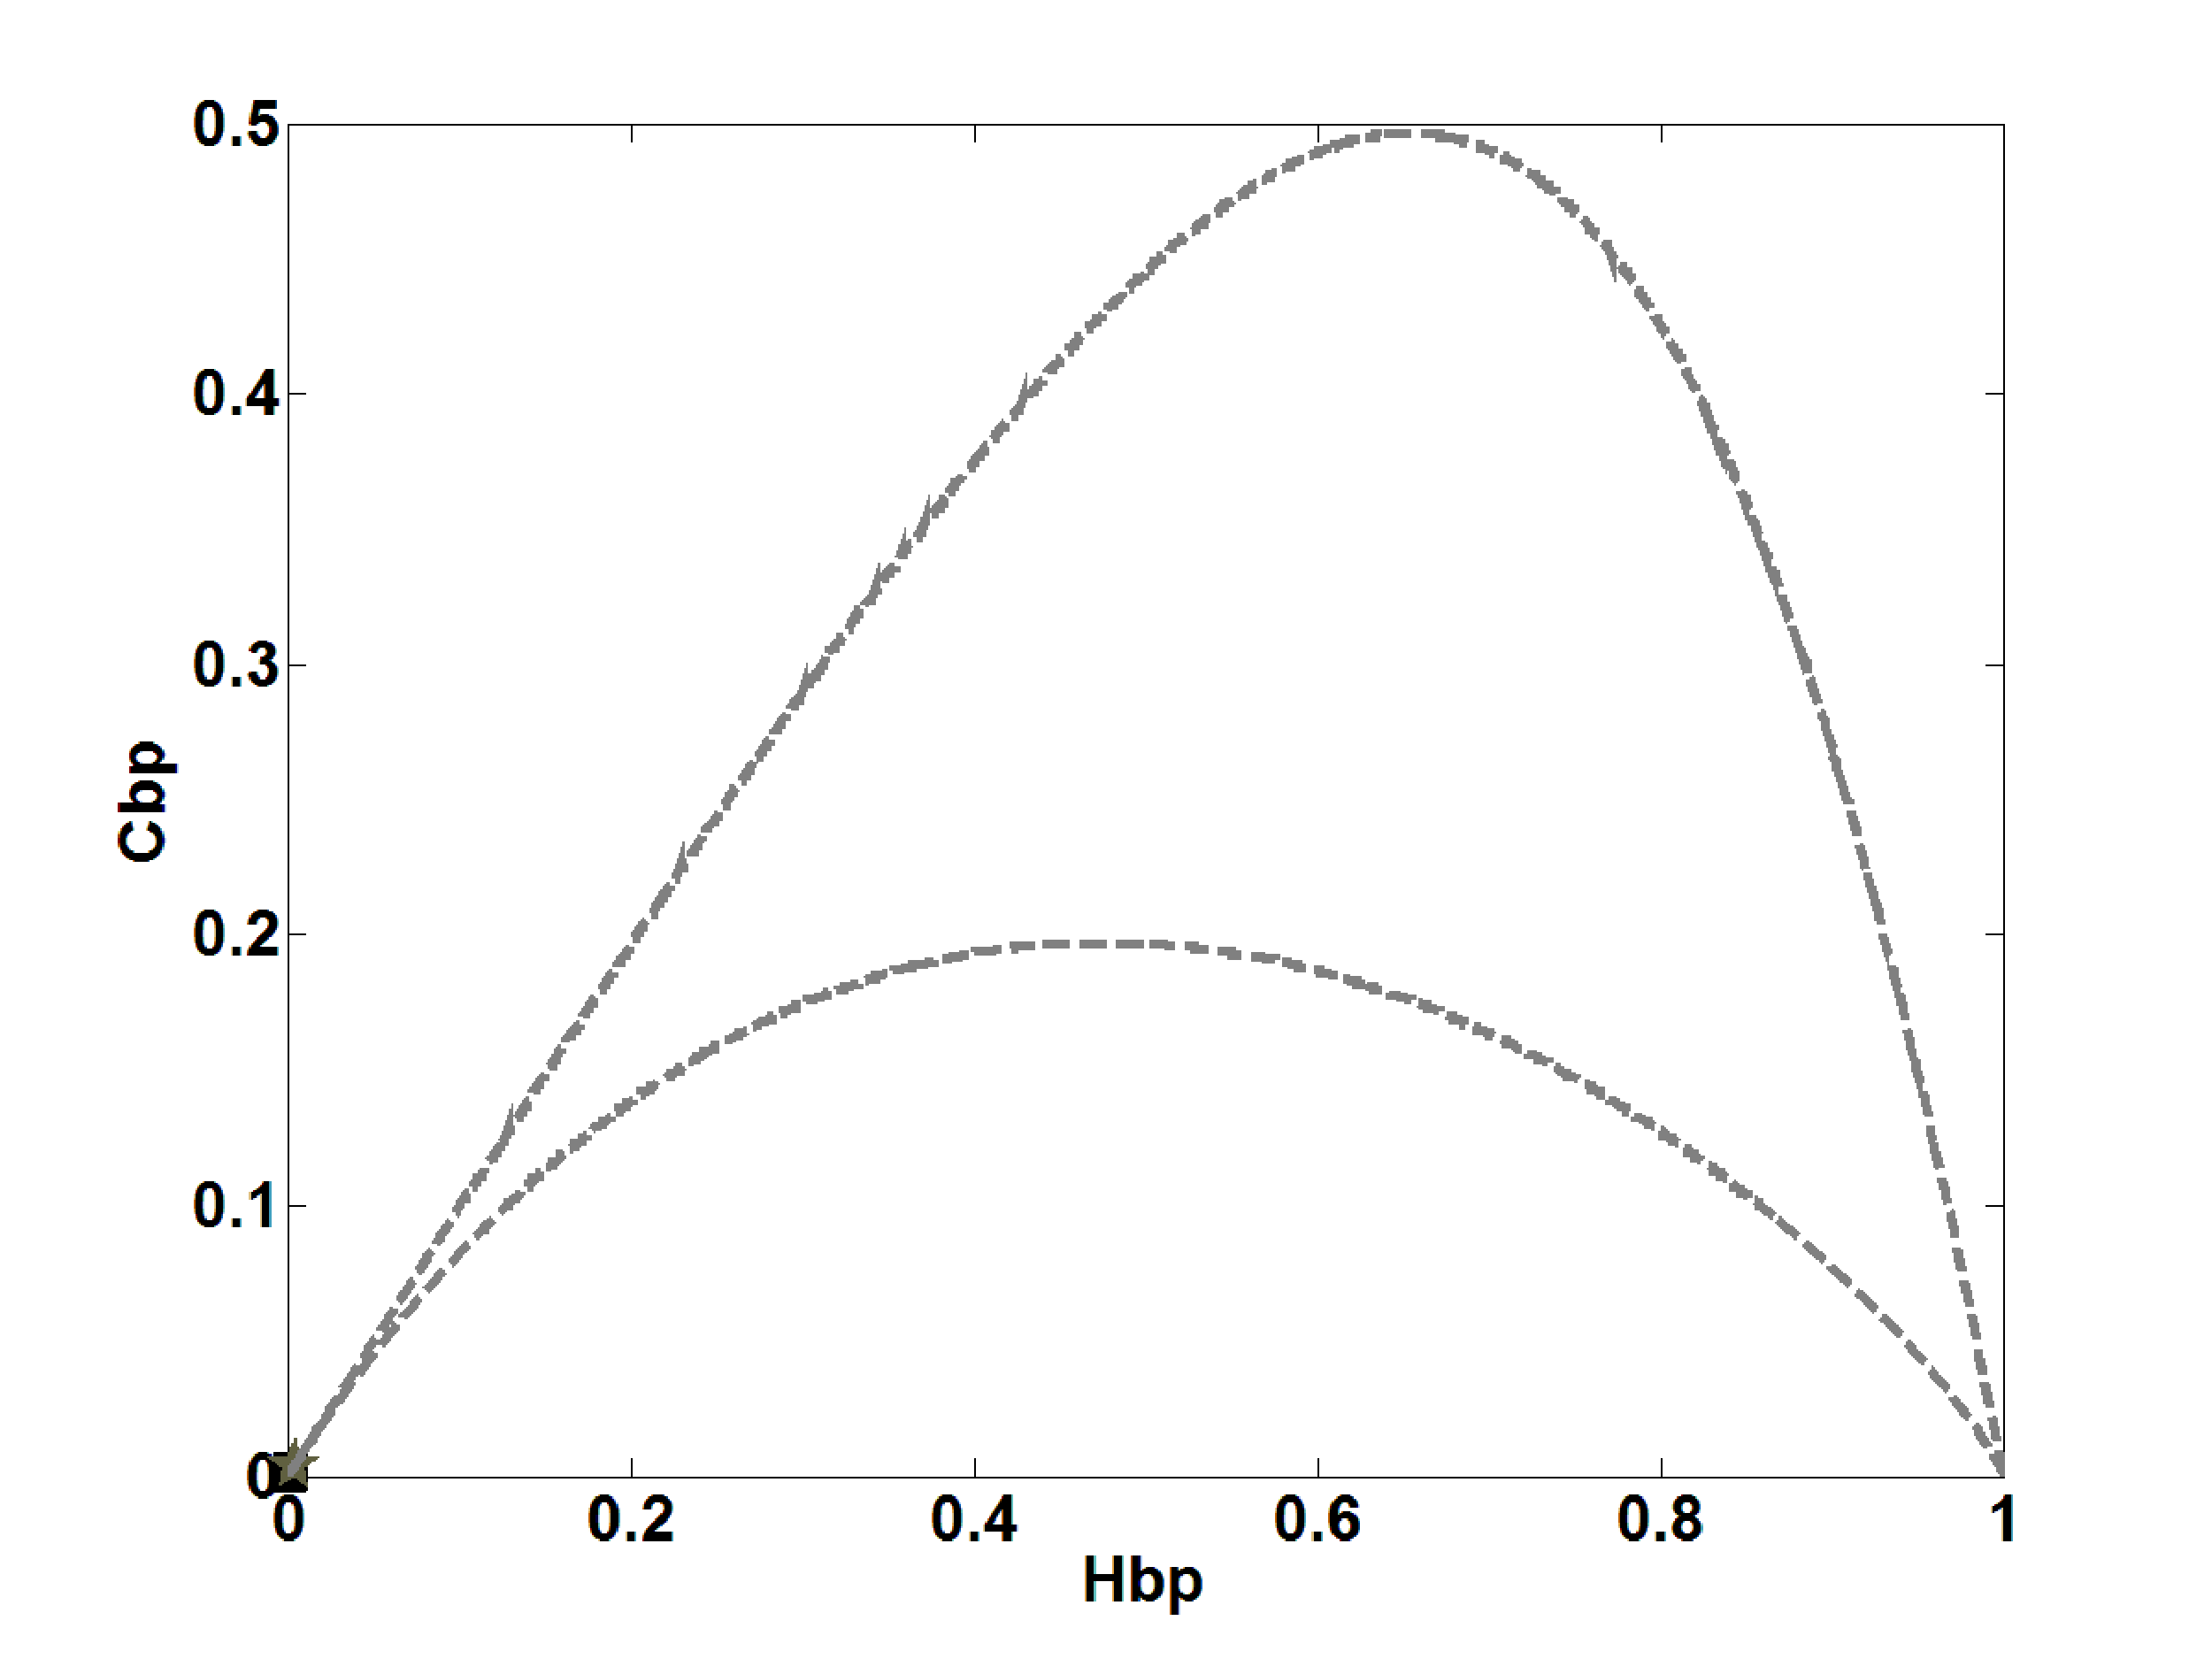
\includegraphics[width=0.3\textwidth]{HbpCbp_tentB2}
\caption{Statistical properties of the Tent map using different numerical representations. Figures (a) to(e) correspond to decimal representation: (a) $H_{hist}$ vs $P$ (b) $H_{BP}$ vs $P$ (c) Number of missing ordering patterns $MP$ vs $P$. In Figures (a) to (c) dashed line correspond to floating point numbers. (d) representation in the $H_{hist},H_{BP}$ plane in the the decimal numerical system.  The star represents the state for floating points numbers. (e) representation in the $H_{BP},C_{BP}$ plane.  The star represents the state for floating points numbers. (f) representation in the $H_{BP},C_{BP}$ plane for binary numerical system.  The star represents the state for floating points numbers. } \label{fig:tent}
\end{figure}

%%%%%%%%%%%%%%%%%%%%%%%%%%
%%%%%%%%%%%%%%%%%%%%%%%%%%% Fig.3
\begin{figure}
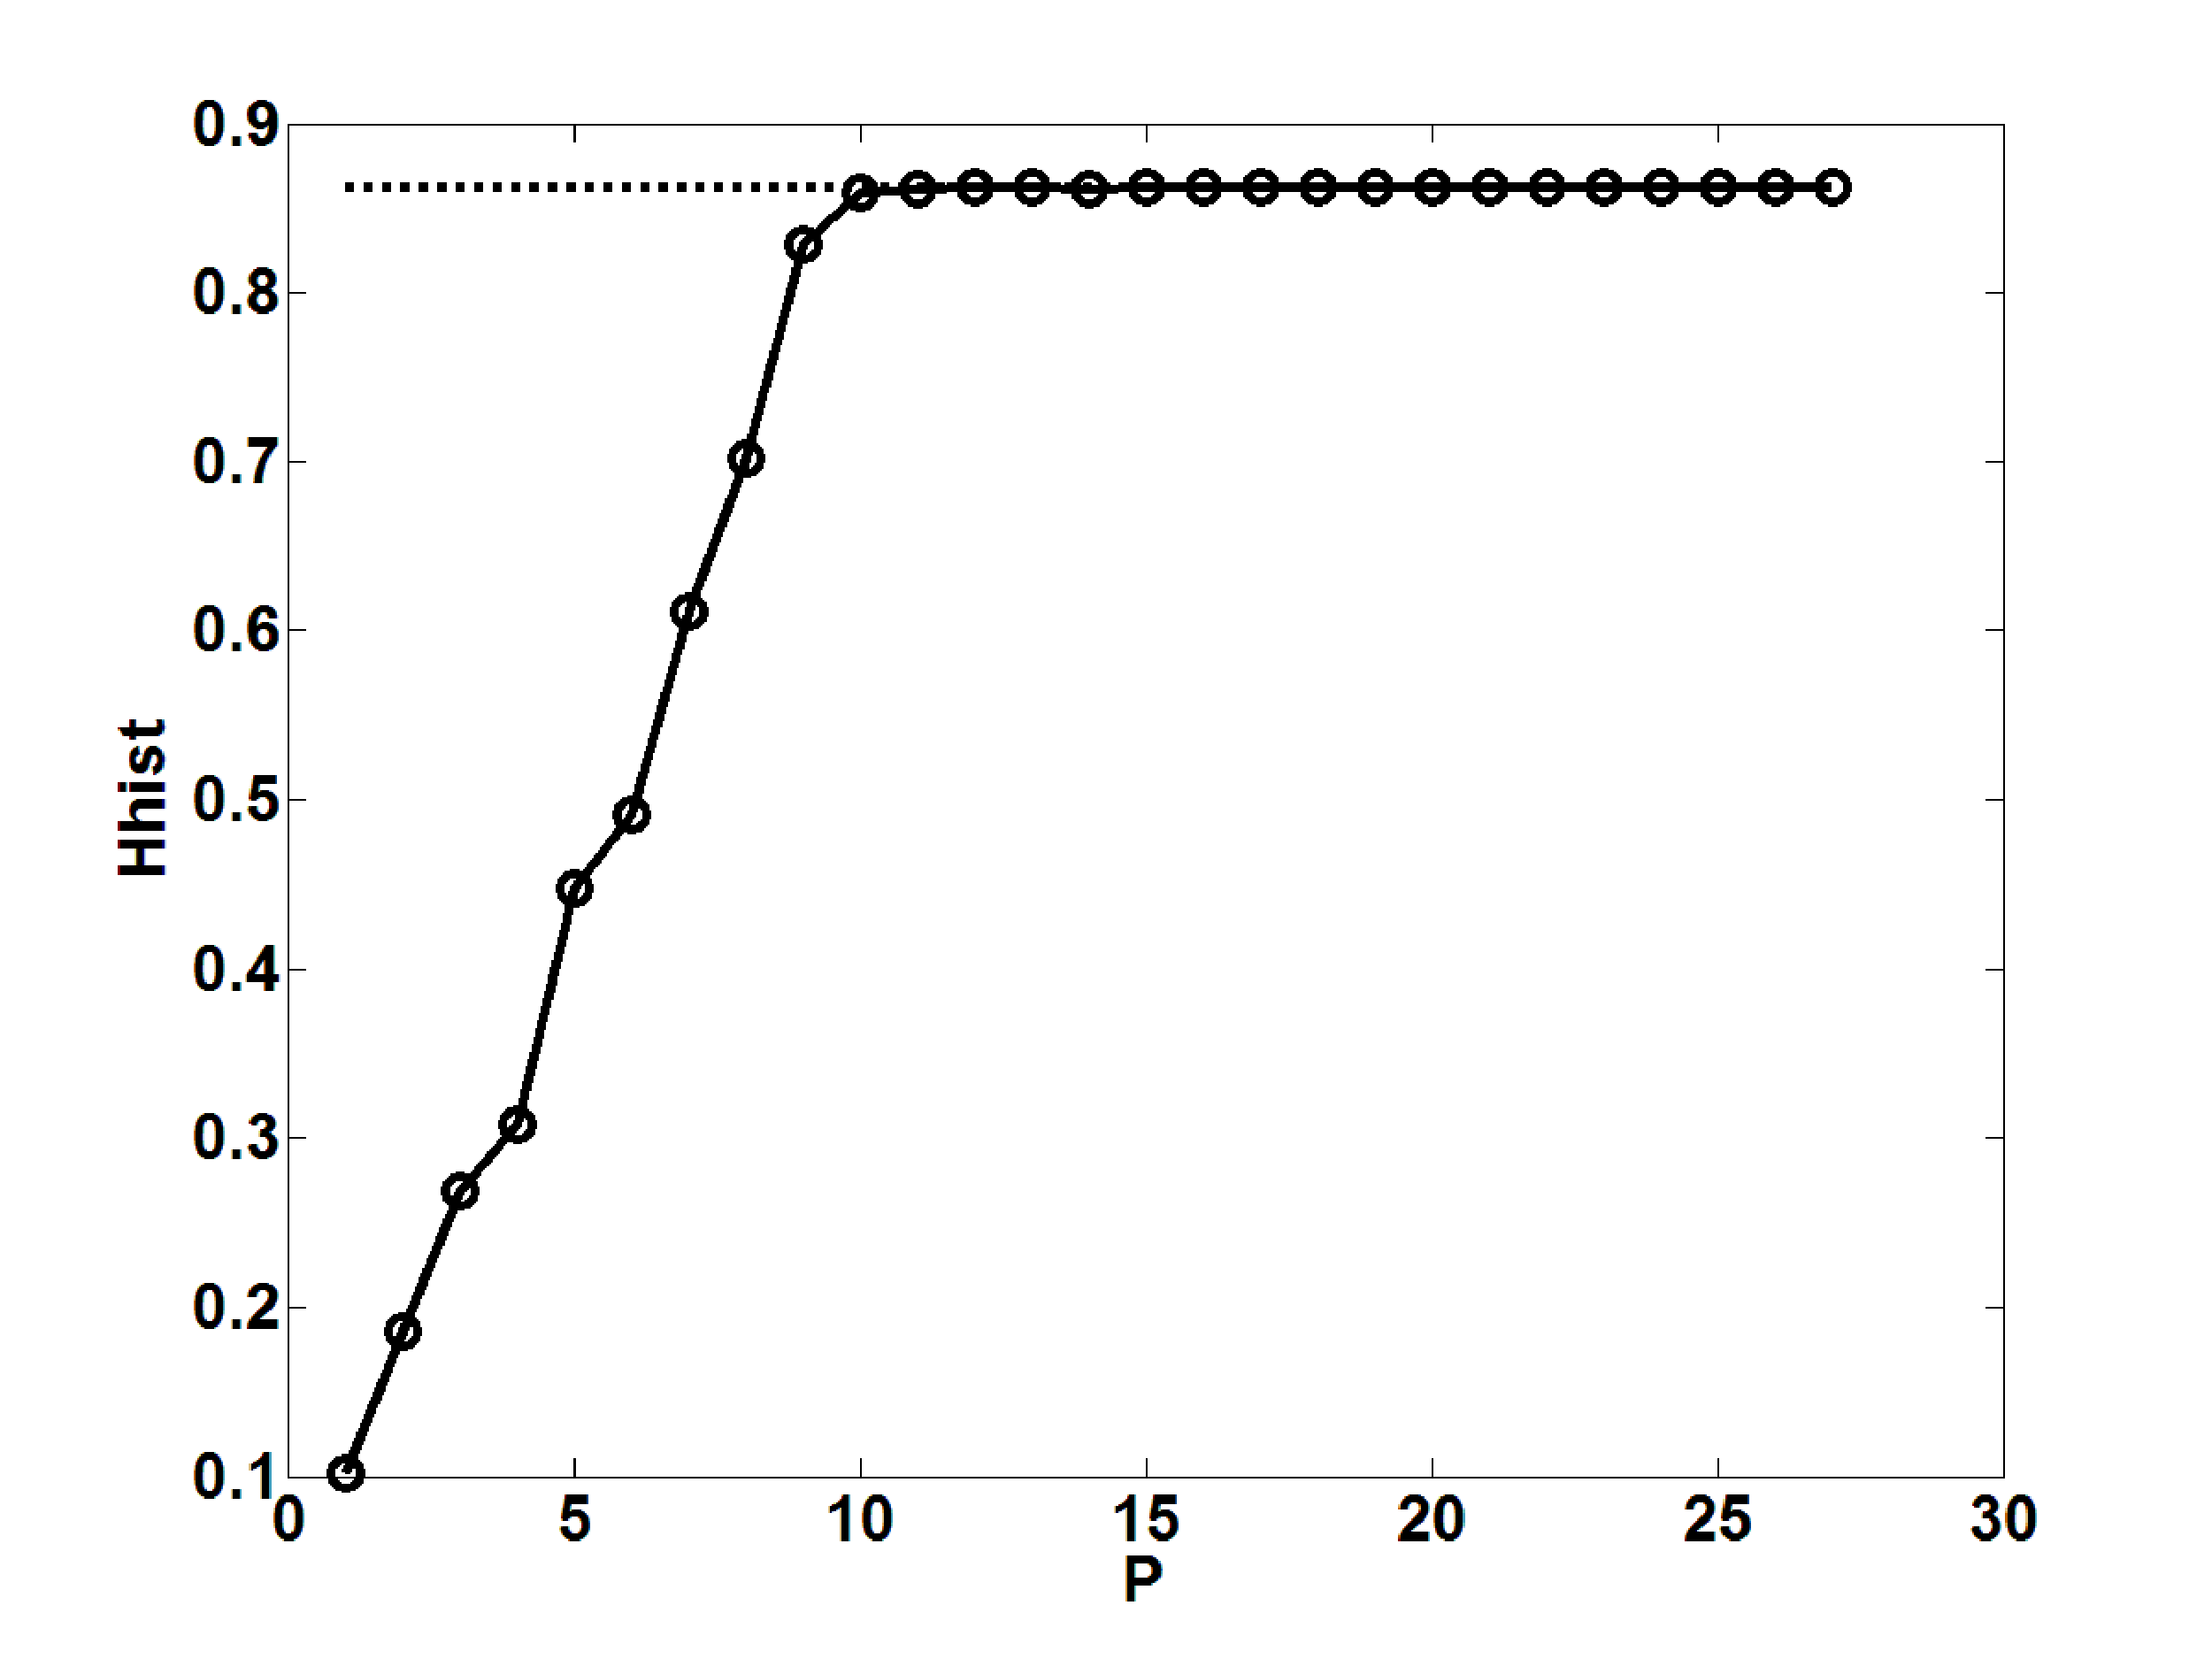
\includegraphics[width=0.3\textwidth]{Hhist_logisticoB10}
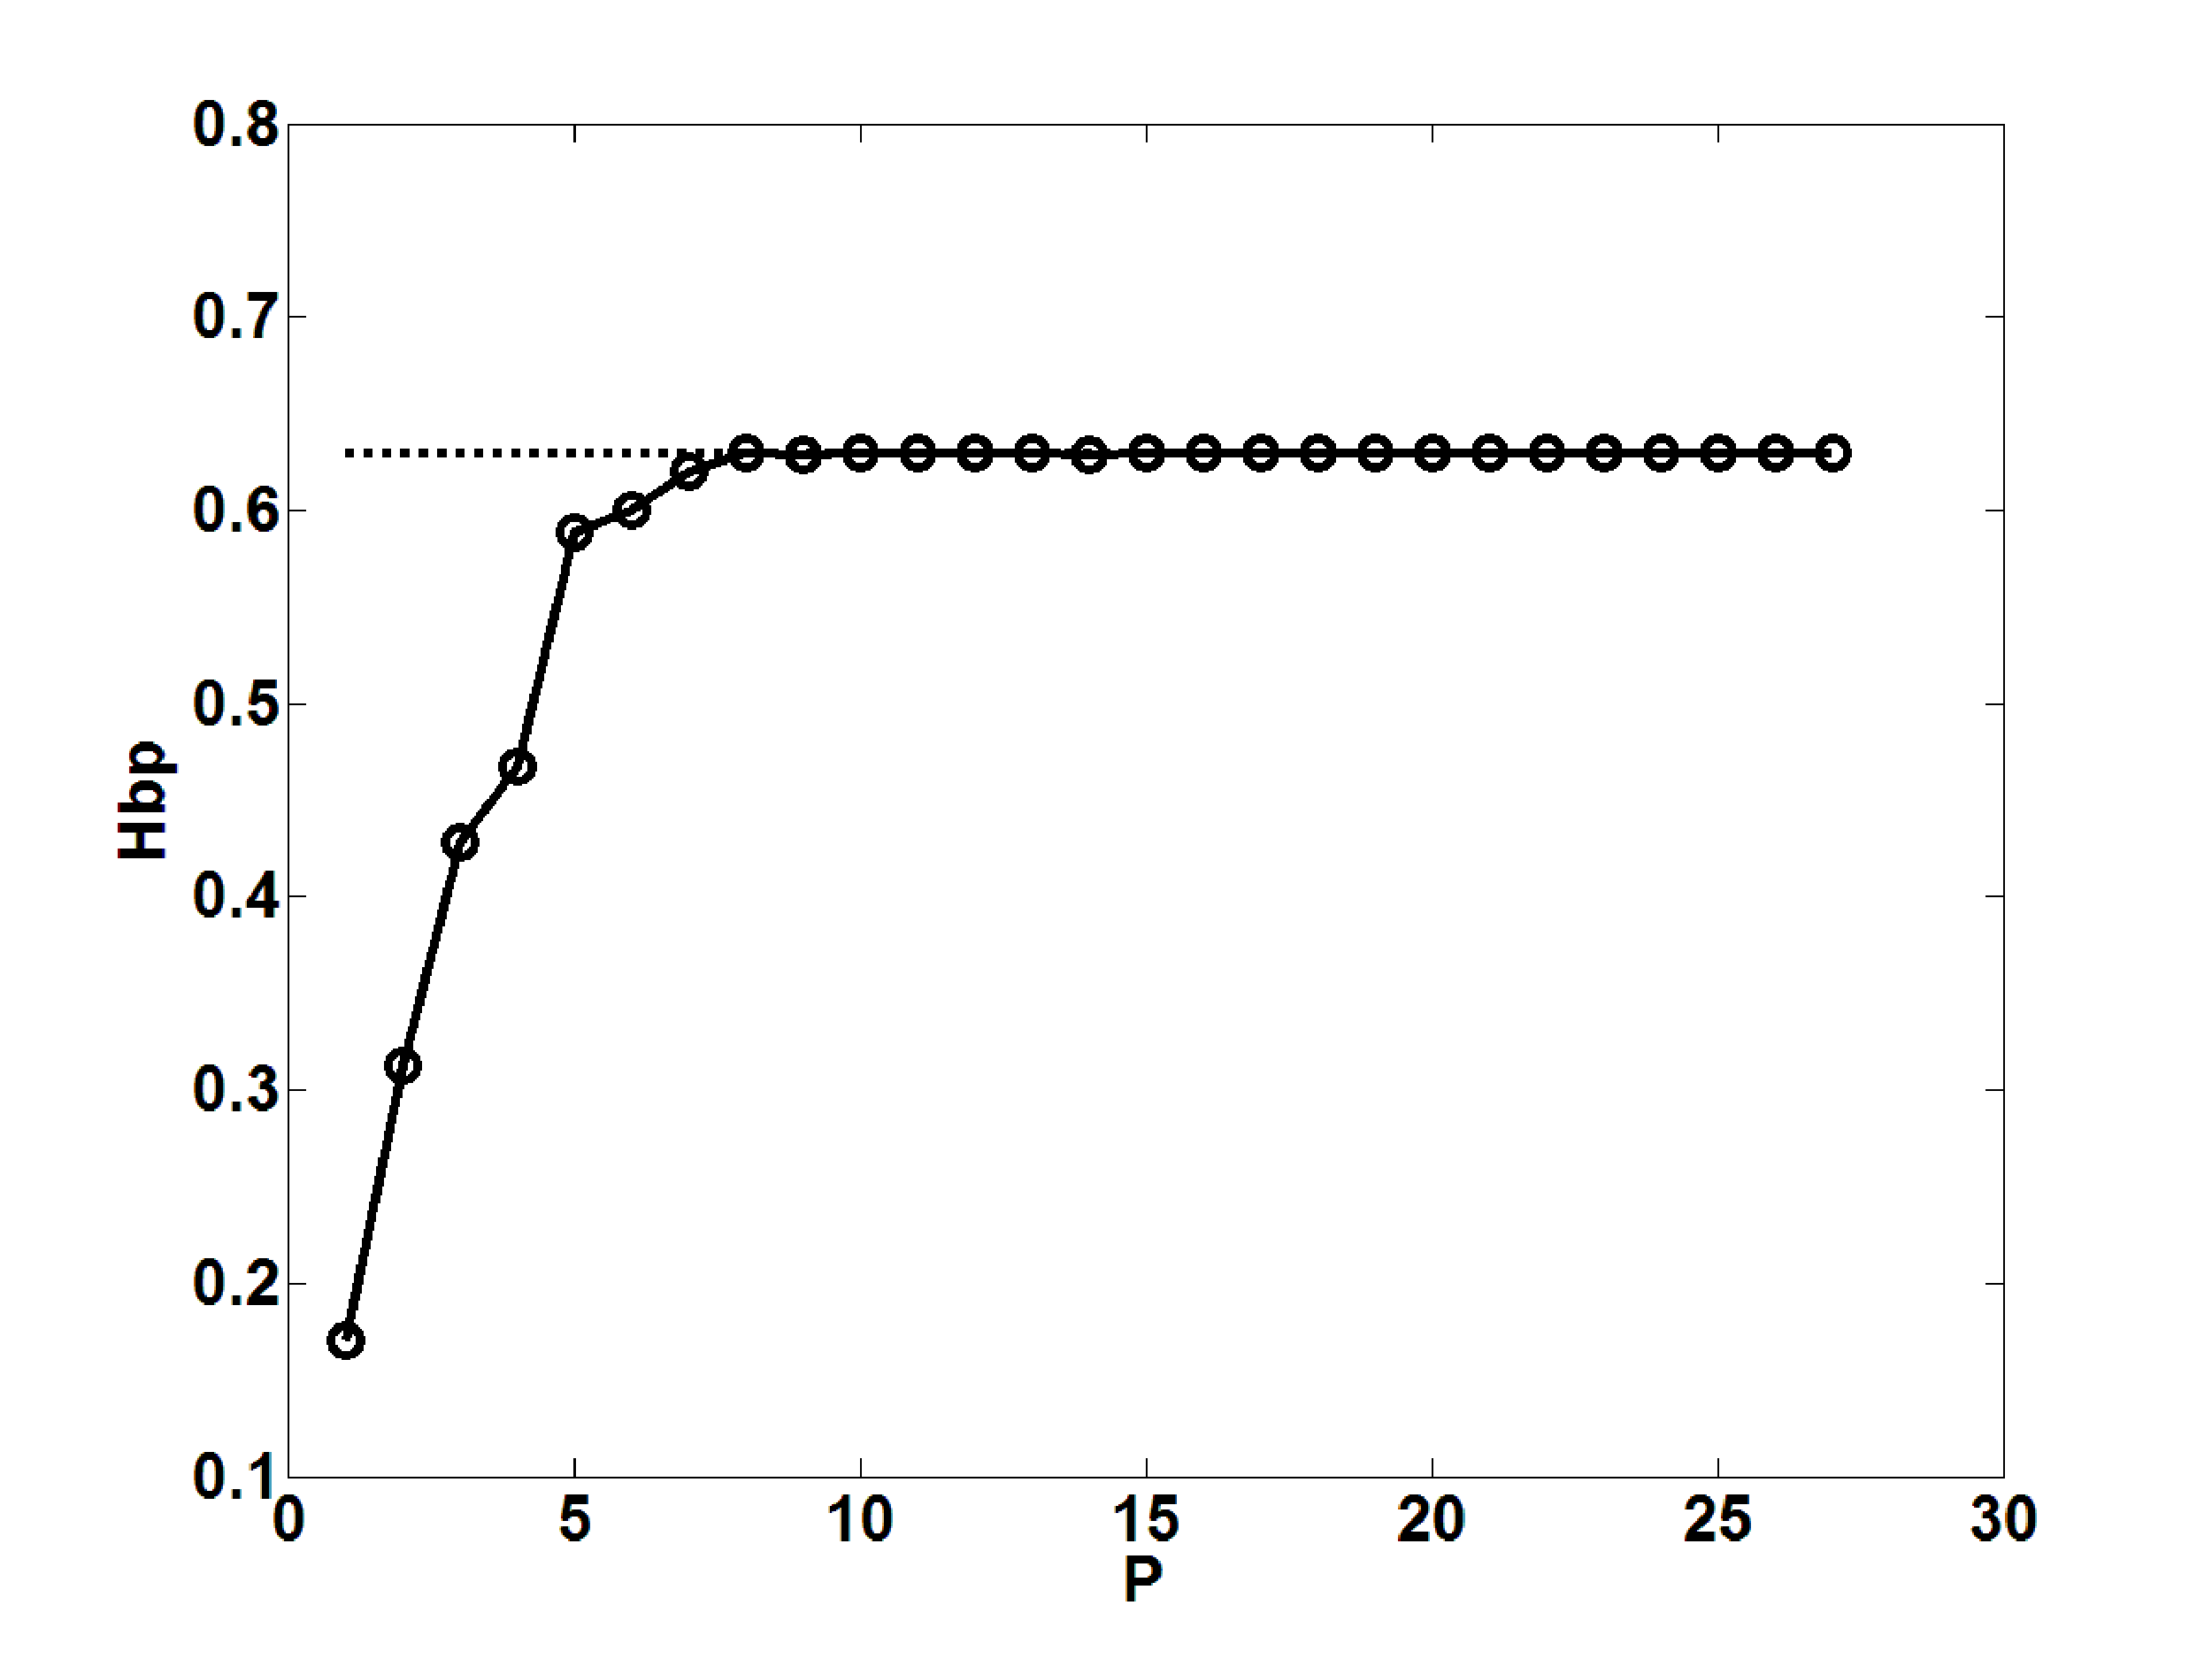
\includegraphics[width=0.3\textwidth]{Hbp_logisticoB10}
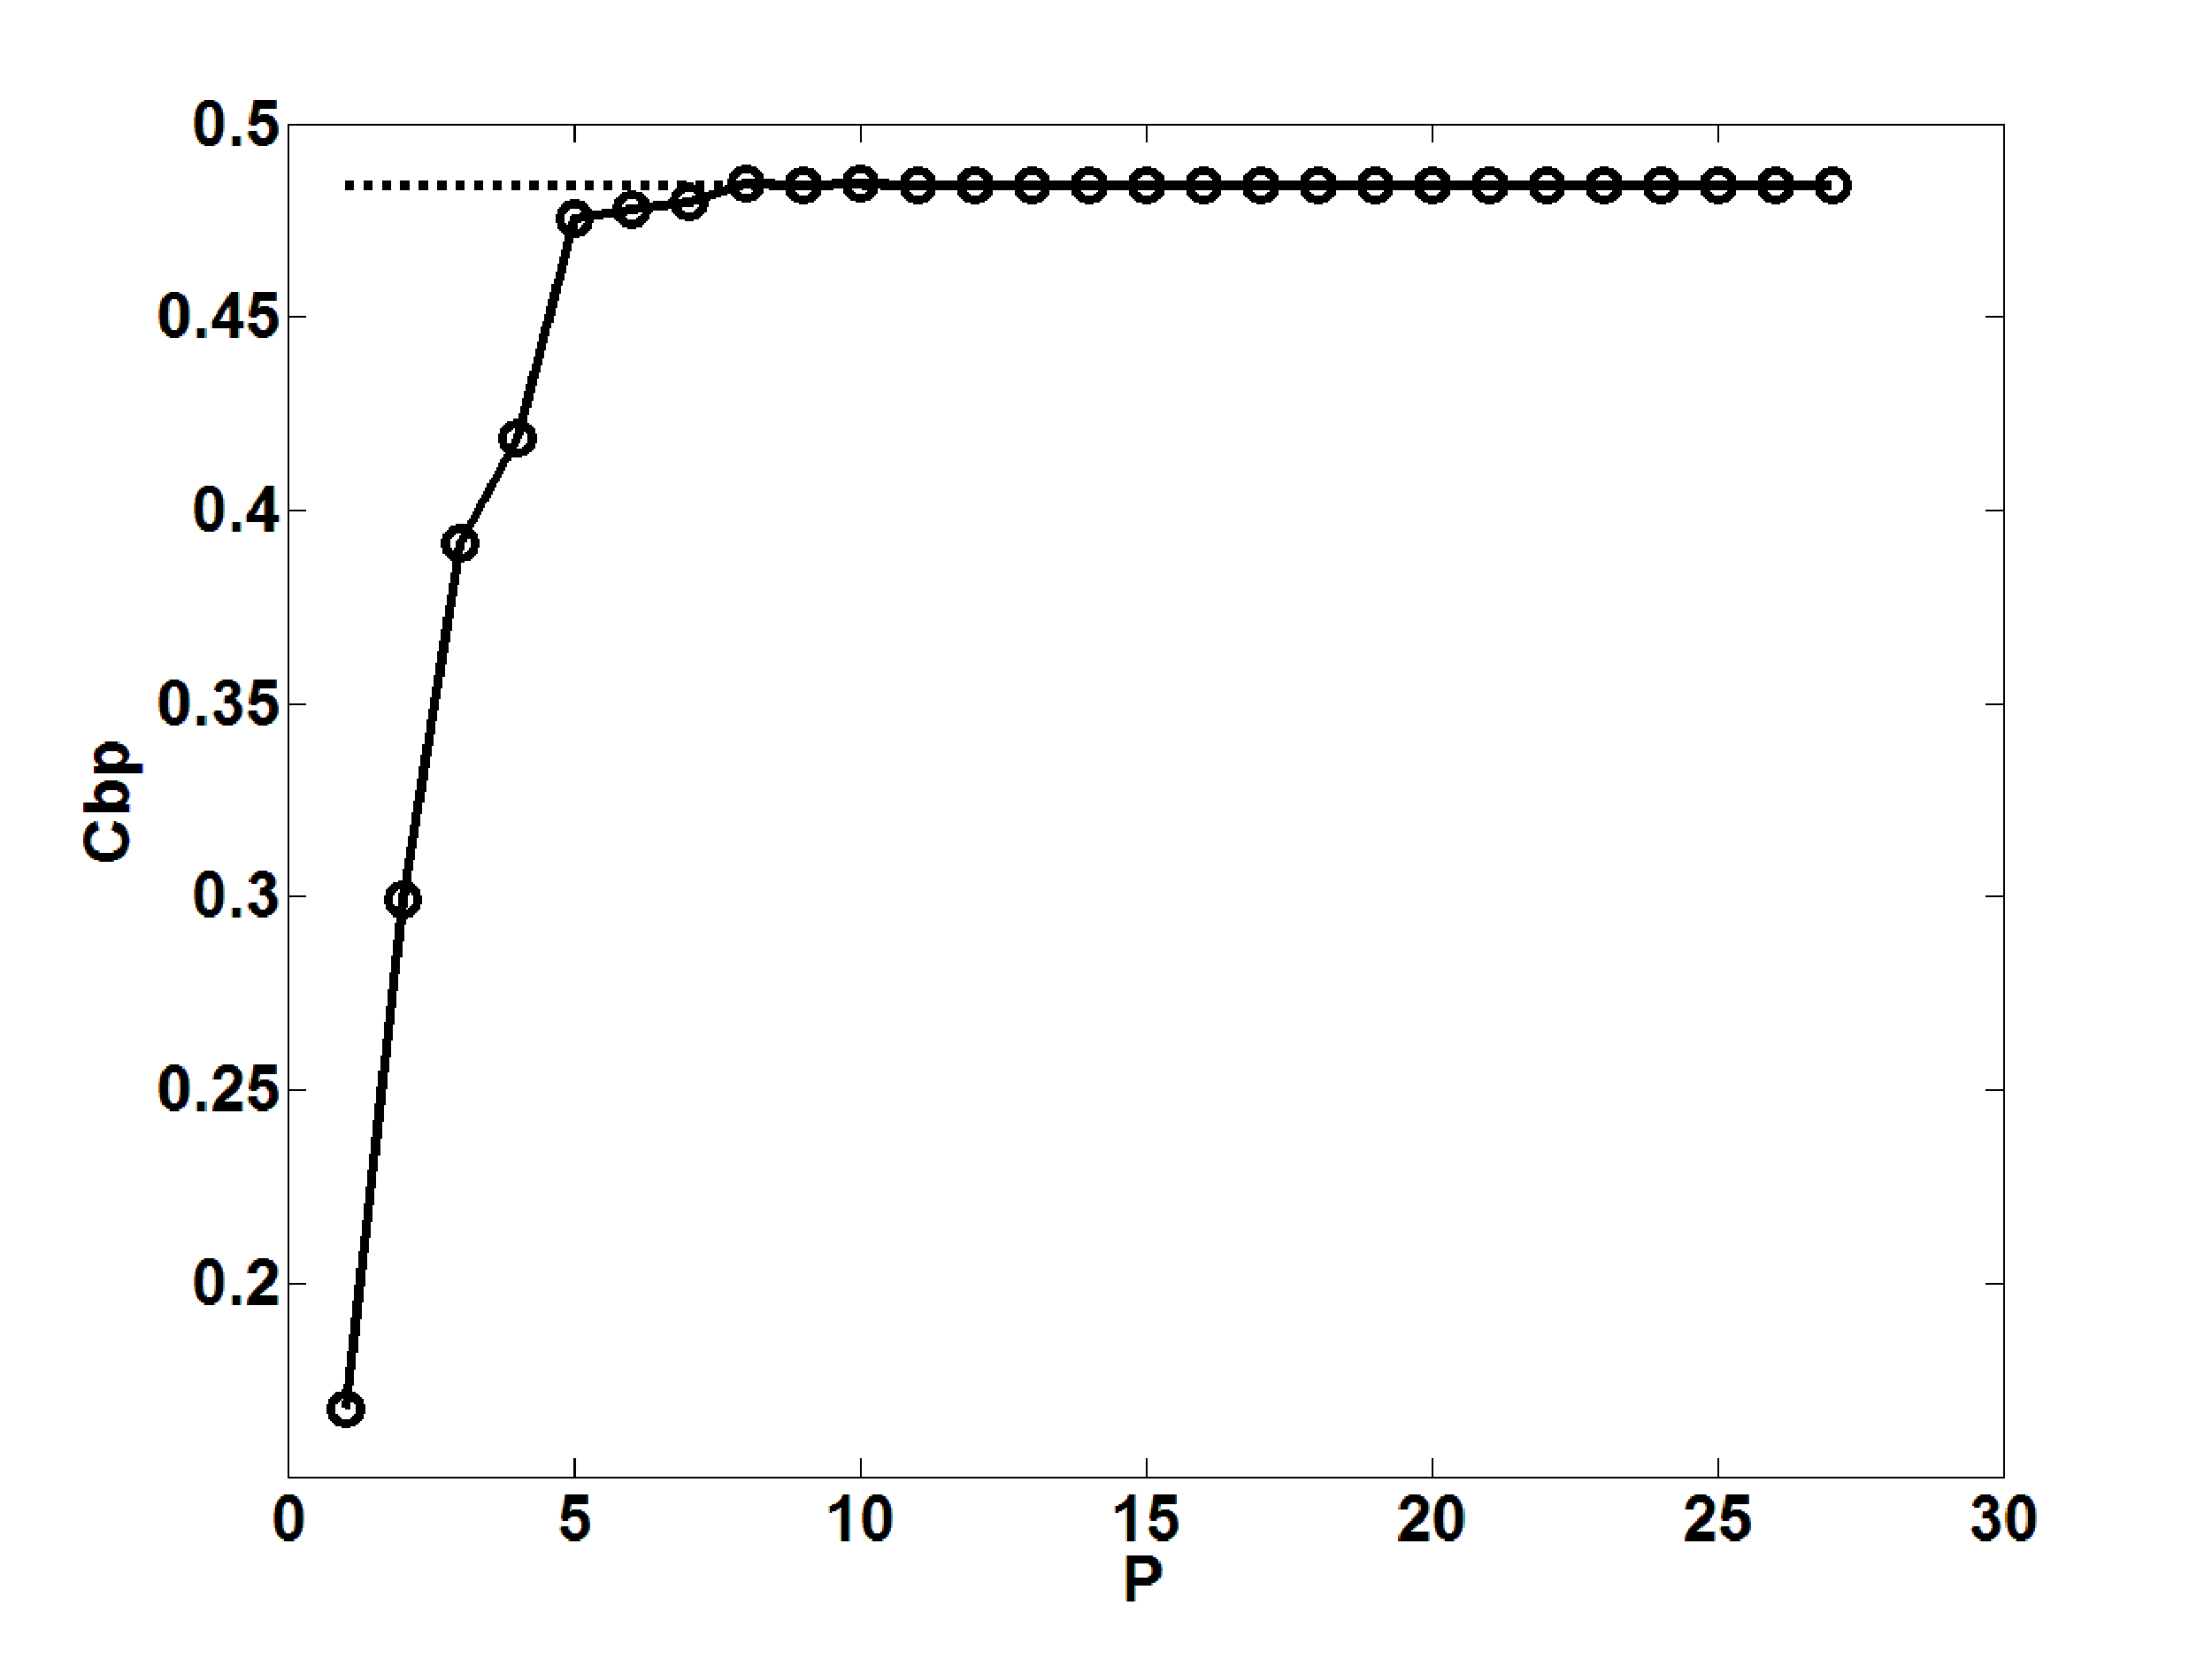
\includegraphics[width=0.3\textwidth]{Cbp_logisticoB10}
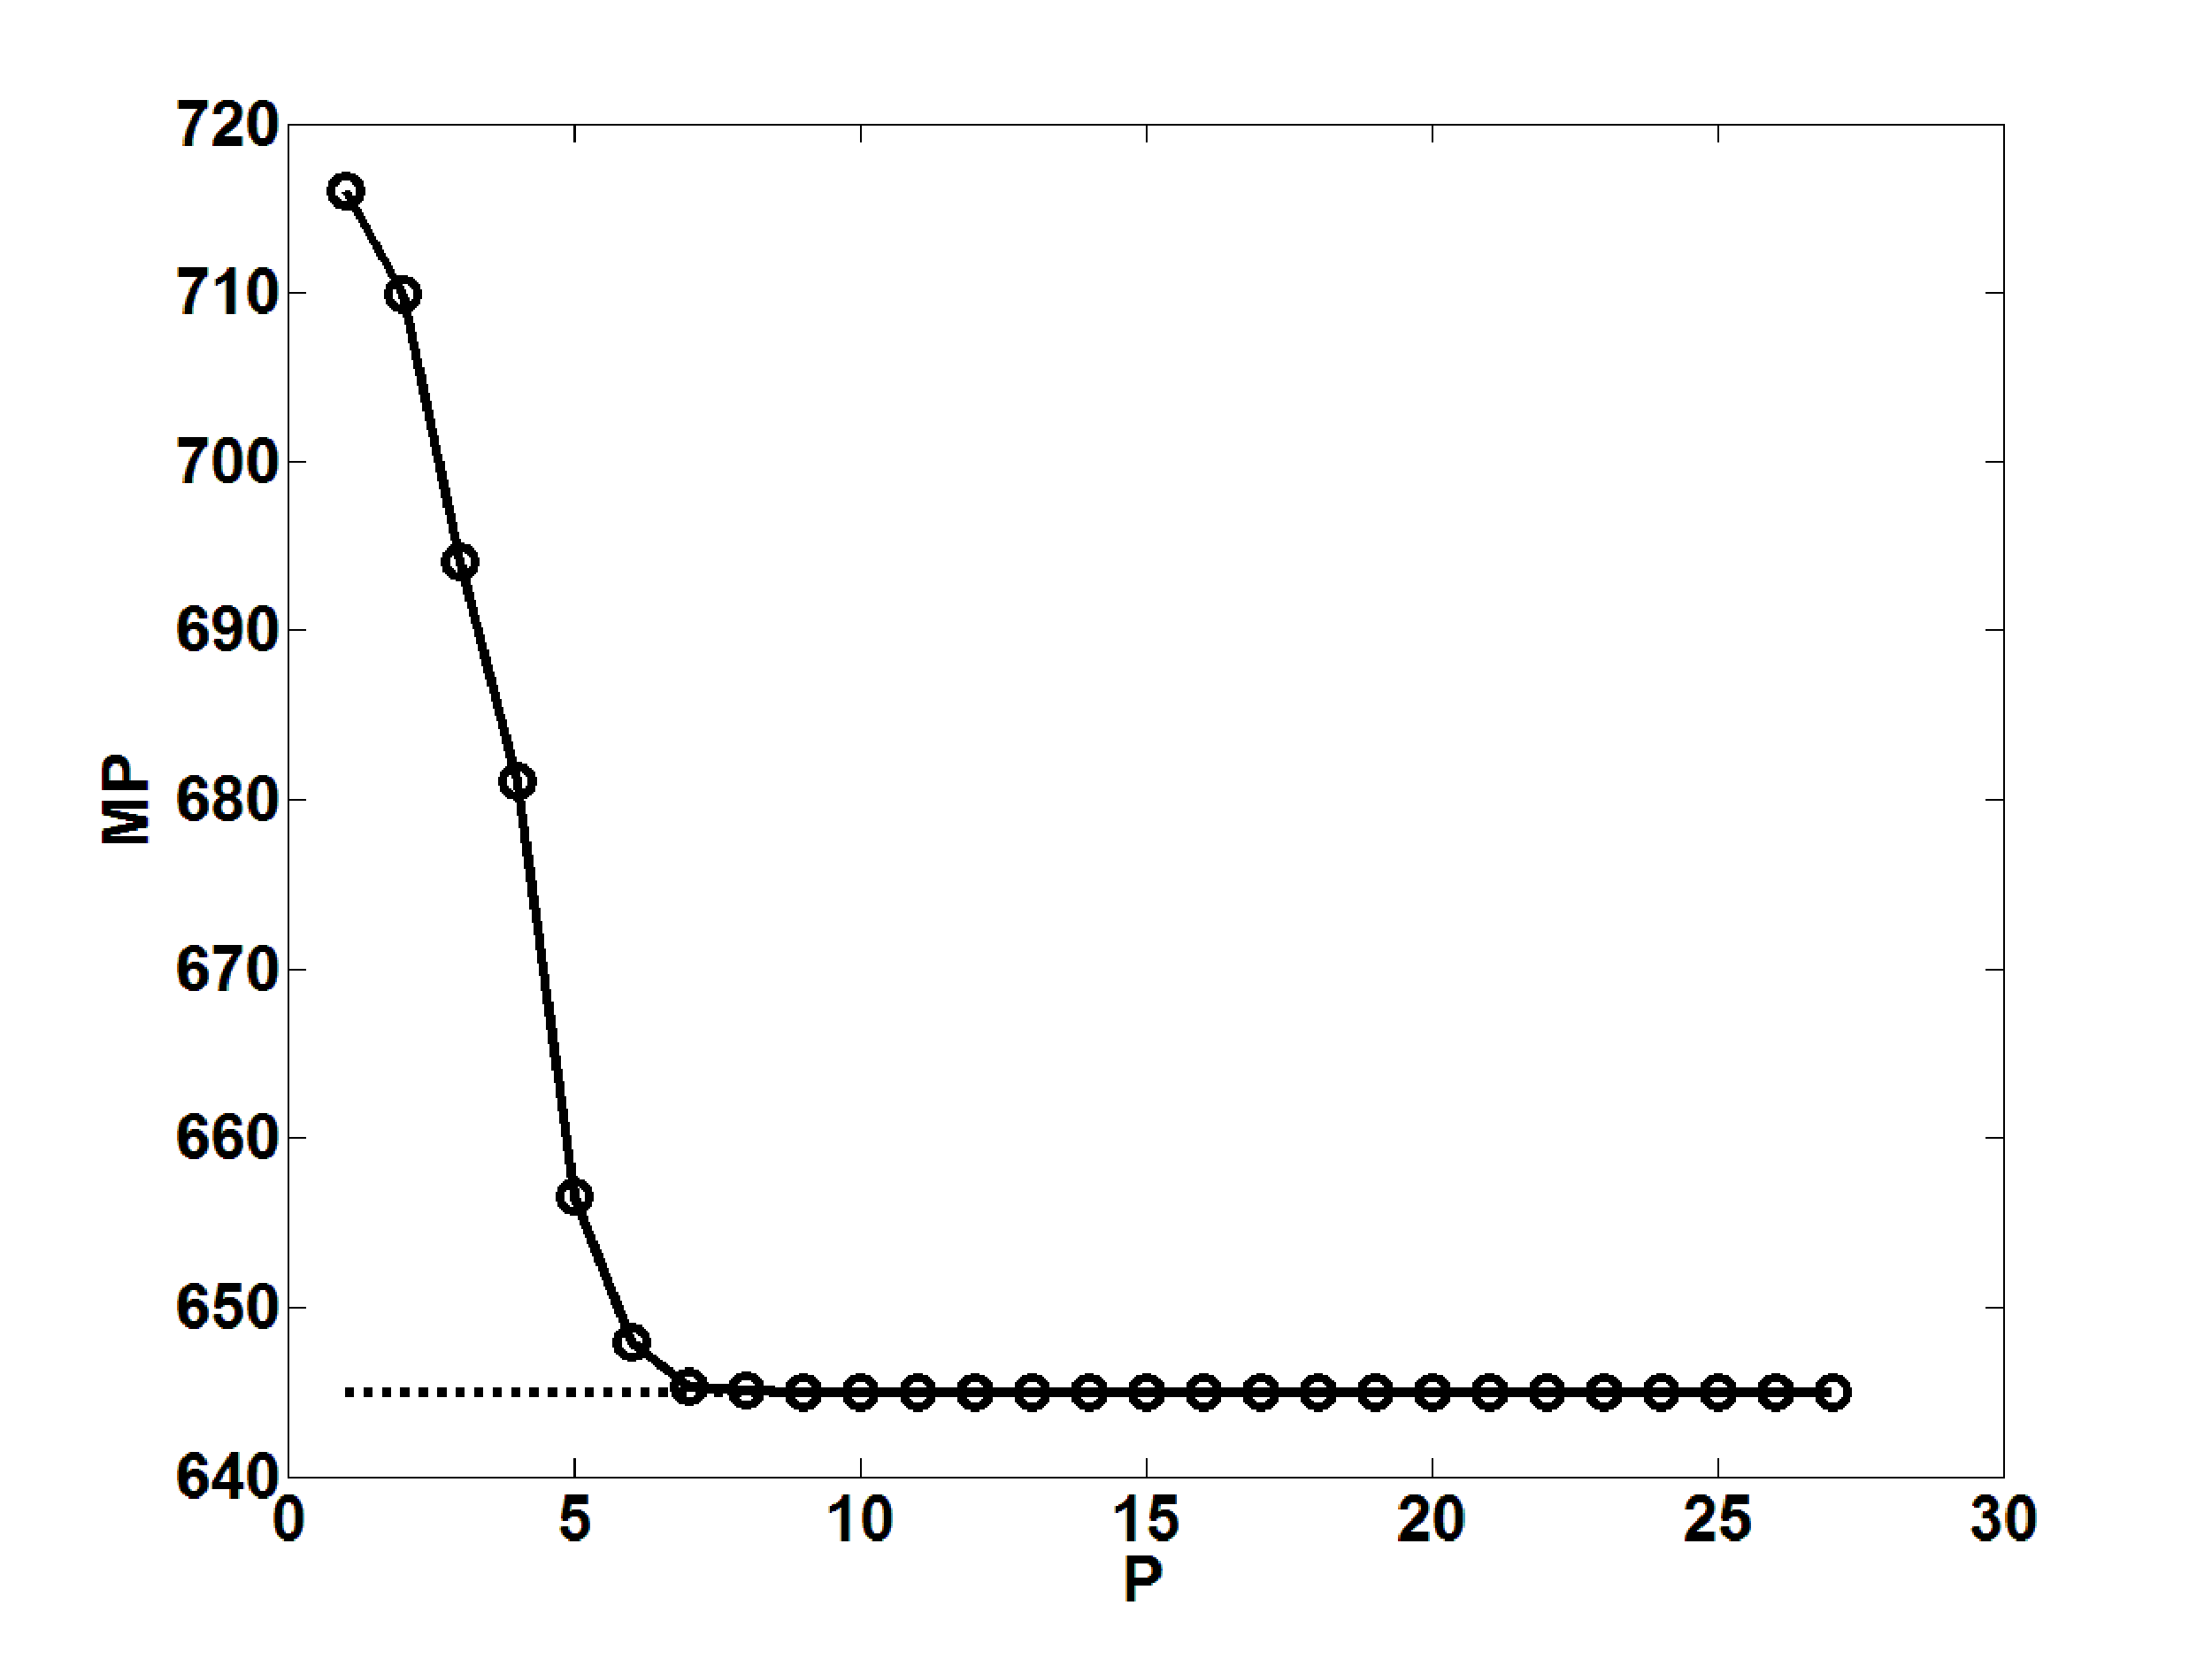
\includegraphics[width=0.3\textwidth]{Miss_logisticoB10}
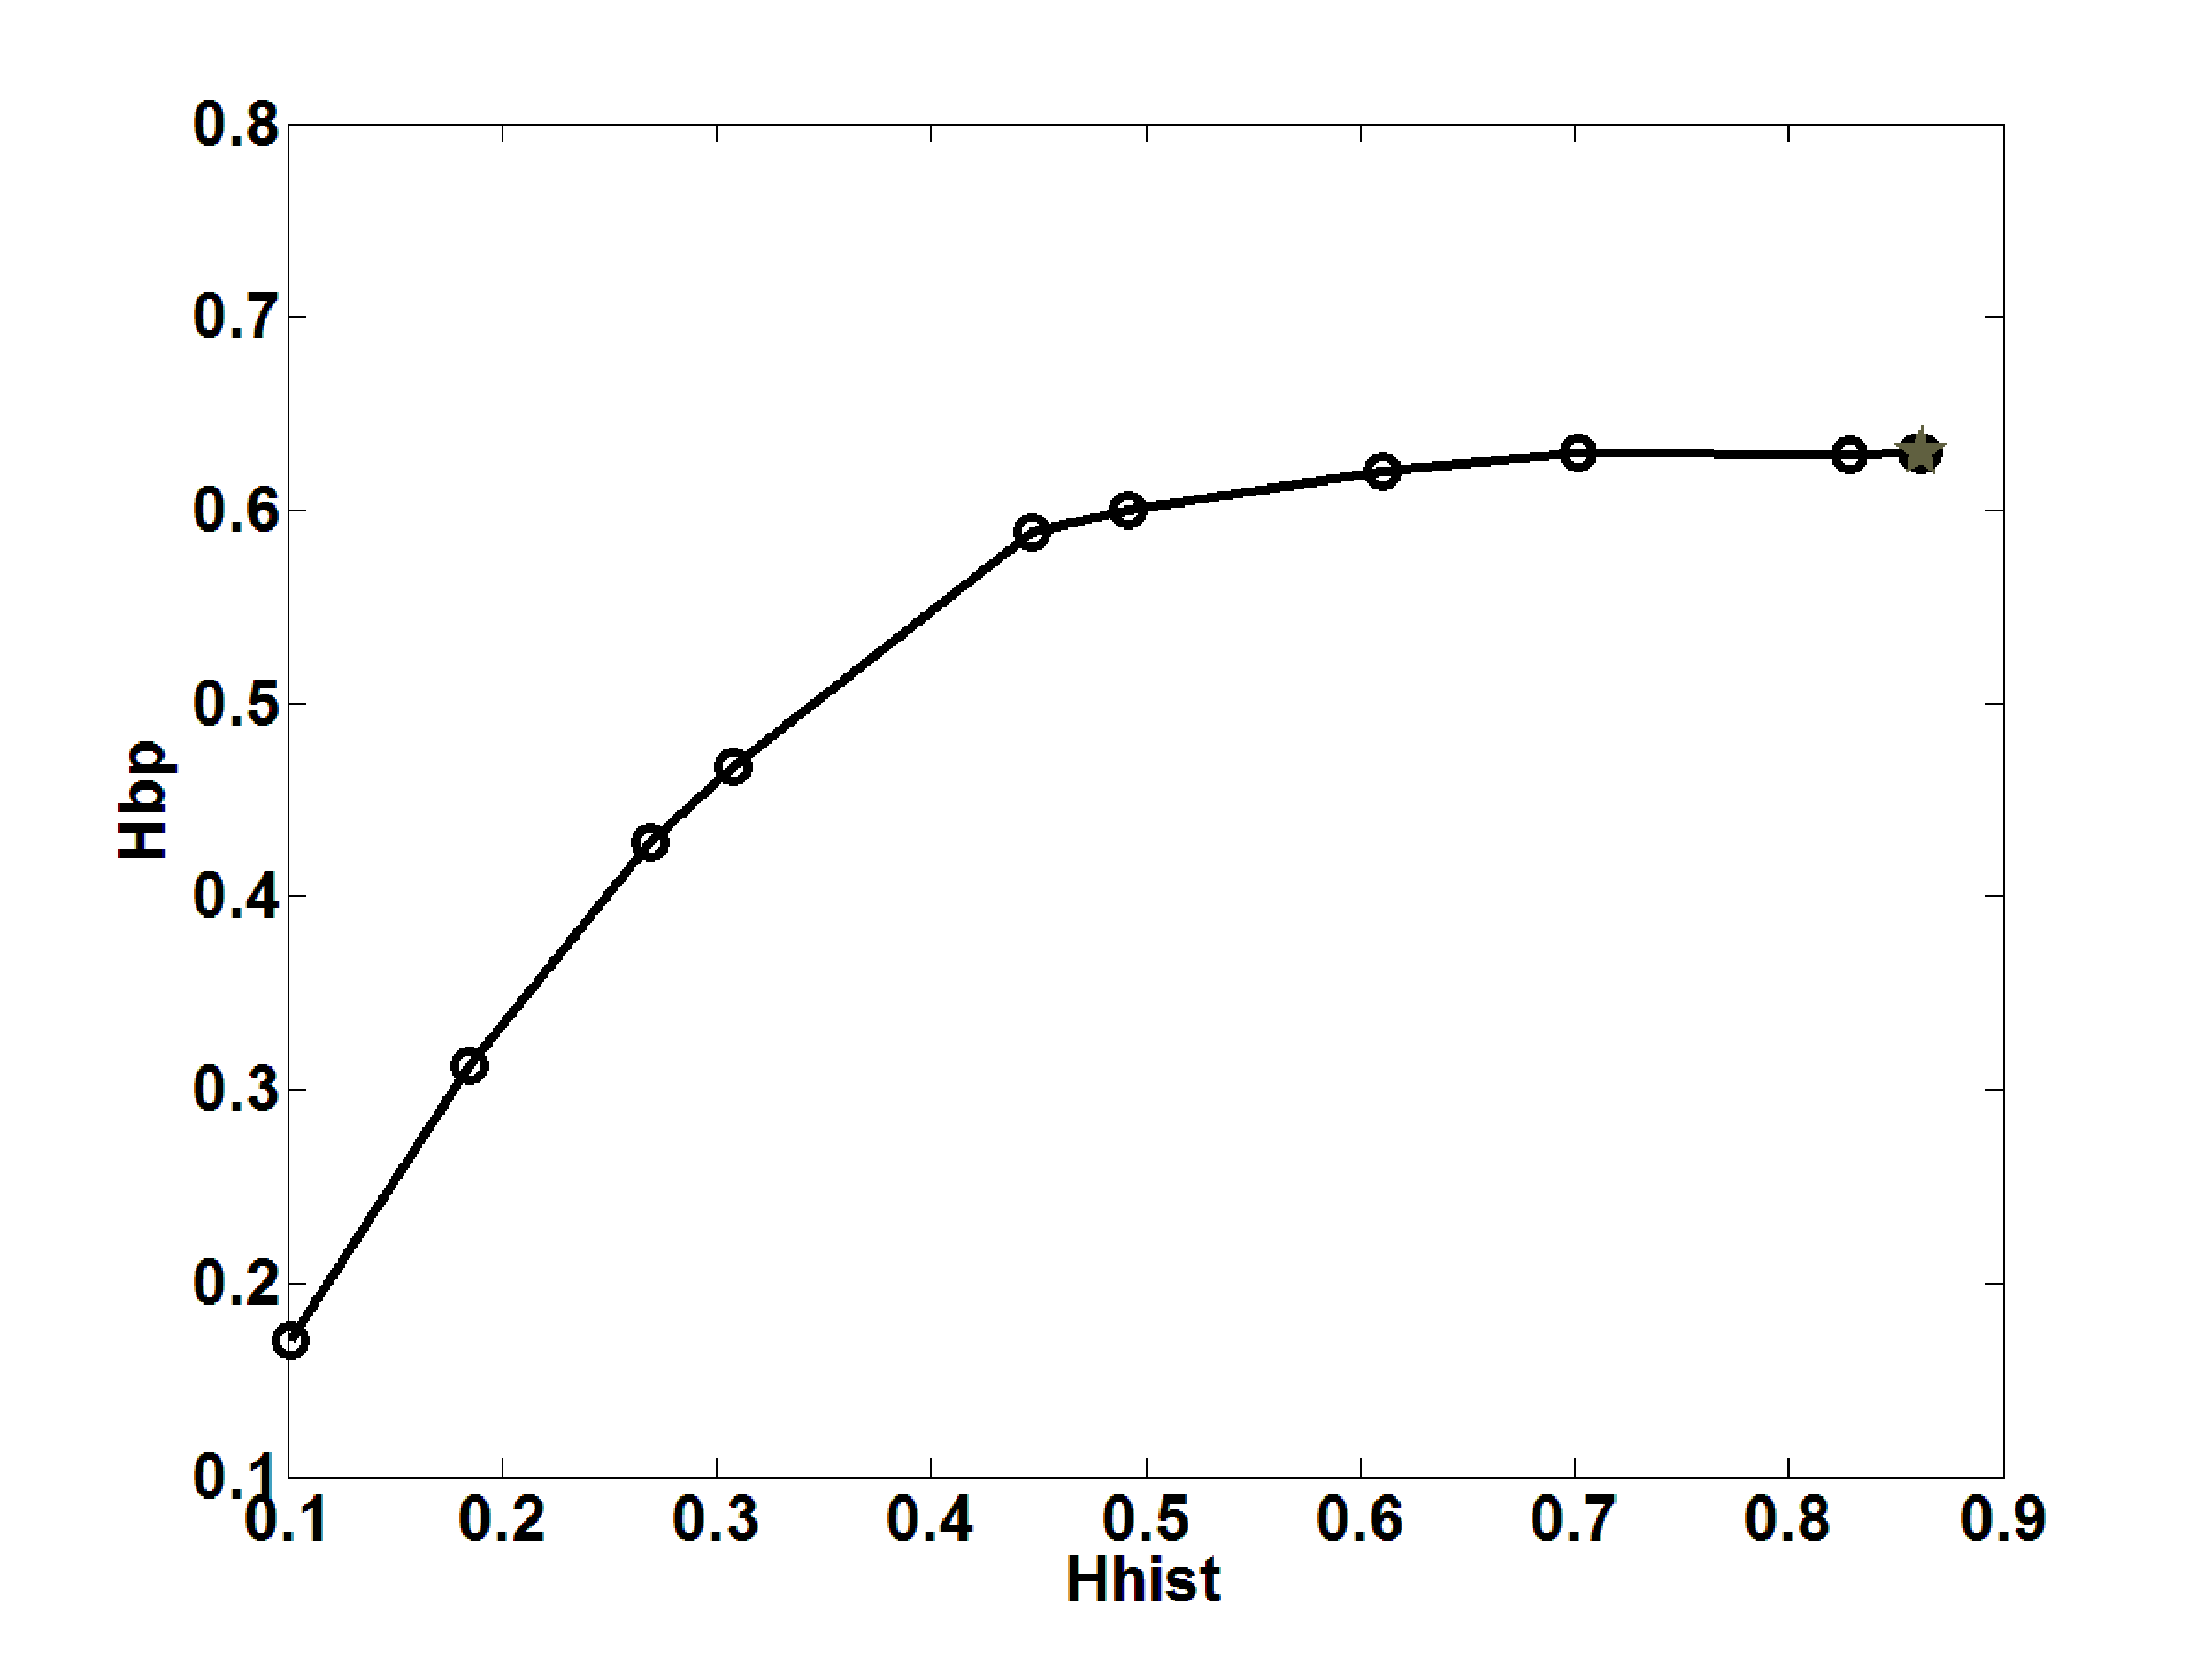
\includegraphics[width=0.3\textwidth]{HhistHbp_logisticoB10}
\includegraphics[width=0.3\textwidth]{HbpCbp_logisticoB10}
\caption{Statistical properties of the LOG map using different numerical representations. Figures (a) to(f) correspond to decimal representation: (a) $H_{hist}$ vs $P$ (b) $H_{BP}$ vs $P$ (c) $C_{BP}$ vs $P$ (d) Number of missing ordering patterns $MP$ vs $P$. In Figures (a) to (d) dashed line correspond to floating point numbers. (d) representation in the $H_{hist},H_{BP}$ plane in the the decimal numerical system.  The star represents the state for floating points numbers. (e) representation in the $H_{hist},H_{BP}$ plane. The star represents the state for floating point numbers; (f) representation in the $H_{BP},C_{BP}$ plane.  The star represents the state for floating points numbers. (f) representation in the $H_{BP},C_{BP}$ plane for binary numerical system.  The star represents the state for floating points numbers. } \label{fig:LOGdecimal}
\end{figure}
%%%%%%%%%%%%%%%%%%%%%%%%%%
%%%%%%%%%%%%%%%%%%%%%%%%%%% Fig.4
\begin{figure}
\includegraphics[width=0.3\textwidth]{Hhist_logisticoB2}
\includegraphics[width=0.3\textwidth]{Hbp_logisticoB2}
\includegraphics[width=0.3\textwidth]{Cbp_logisticoB2}
\includegraphics[width=0.3\textwidth]{Miss_logisticoB2}
\includegraphics[width=0.3\textwidth]{HhistHbp_logisticoB2}
\includegraphics[width=0.3\textwidth]{HbpCbp_logisticoB2}
\caption{Statistical properties of the LOG map using binary representation: (a) $H_{hist}$ vs $P$ (b) $H_{BP}$ vs $P$ (c) $C_{BP}$ vs $P$ (d) Number of missing ordering patterns $MP$ vs $P$. In Figures (a) to (d) dashed line correspond to floating point numbers. (d) representation in the $H_{hist},H_{BP}$ plane in the the decimal numerical system.  The star represents the state for floating points numbers. (e) representation in the $H_{hist},H_{BP}$ plane. The star represents the state for floating point numbers; (f) representation in the $H_{BP},C_{BP}$ plane.  The star represents the state for floating points numbers. (f) representation in the $H_{BP},C_{BP}$ plane for binary numerical system.  The star represents the state for floating points numbers. } \label{fig:LOGbinario}
\end{figure}

%%%%%%%%%%%%%%%%%%%%%%%%%%
%%%%%%%%%%%%%%%%%%%%%%%%%%% Fig.5
\begin{figure}
\includegraphics[width=0.3\textwidth]{Hhist_switchB10}
\includegraphics[width=0.3\textwidth]{Hbp_switchB10}
\includegraphics[width=0.3\textwidth]{Cbp_switchB10}
\includegraphics[width=0.3\textwidth]{Miss_switchB10}
\includegraphics[width=0.3\textwidth]{HhistHbp_switchB10}
\includegraphics[width=0.3\textwidth]{HbpCbp_switchB10}
\caption{Statistical properties of the SWITCH map using decimal representation: (a) $H_{hist}$ vs $P$ (b) $H_{BP}$ vs $P$ (c) $C_{BP}$ vs $P$ (d) Number of missing ordering patterns $MP$ vs $P$. In Figures (a) to (d) dashed line correspond to floating point numbers. (e) representation in the $H_{hist},H_{BP}$ plane in the the decimal numerical system.  The star represents the state for floating points numbers. (f) representation in the $H_{BP},C_{BP}$ plane.  The star represents the state for floating points numbers. (The star represents the state for floating points numbers). } \label{fig:seqdec}
\end{figure}

%%%%%%%%%%%%%%%%%%%%%%%%%%
%%%%%%%%%%%%%%%%%%%%%%%%%%% Fig.6
\begin{figure}
\includegraphics[width=0.3\textwidth]{Hhist_switchB2}
\includegraphics[width=0.3\textwidth]{Hbp_switchB2}
\includegraphics[width=0.3\textwidth]{Cbp_switchB2}
\includegraphics[width=0.3\textwidth]{Miss_switchB2}
\includegraphics[width=0.3\textwidth]{HhistHbp_switchB2}
\includegraphics[width=0.3\textwidth]{HbpCbp_switchB2}
\caption{Statistical properties of the SWITCH map using binary representation: (a) $H_{hist}$ vs $P$ (b) $H_{BP}$ vs $P$ (c) $C_{BP}$ vs $P$ (d) Number of missing ordering patterns $MP$ vs $P$. In Figures (a) to (d) dashed line correspond to floating point numbers. (e) representation in the $H_{hist},H_{BP}$ plane in the the binary numerical system.  The star represents the state for floating points numbers. (f) representation in the $H_{BP},C_{BP}$ plane.  The star represents the state for floating points numbers. (The star represents the state for floating points numbers). } \label{fig:seqbin}
\end{figure}

%%%%%%%%%%%%%%%%%%%%%%%%%%
%%%%%%%%%%%%%%%%%%%%%%%%%%% Fig.7
\begin{figure}
\includegraphics[width=0.3\textwidth]{Hhist_parB10}
\includegraphics[width=0.3\textwidth]{Hbp_parB10}
\includegraphics[width=0.3\textwidth]{Cbp_parB10}
\includegraphics[width=0.3\textwidth]{Miss_parB10}
\includegraphics[width=0.3\textwidth]{HhistHbp_parB10}
\includegraphics[width=0.3\textwidth]{HbpCbp_parB10}
\caption{Statistical properties of EVEN, obtained by skipping the values in the odd position of the time series of  SWITCH,  using decimal representation: (a) $H_{hist}$ vs $P$ (b) $H_{BP}$ vs $P$ (c) $C_{BP}$ vs $P$ (d) Number of missing ordering patterns $MP$ vs $P$. In Figures (a) to (d) dashed line correspond to floating point numbers. (e) representation in the $H_{hist},H_{BP}$ plane in the the decimal numerical system.  The star represents the state for floating points numbers. (f) representation in the $H_{BP},C_{BP}$ plane.  The star represents the state for floating points numbers. } \label{fig:seqpardec}
\end{figure}

%%%%%%%%%%%%%%%%%%%%%%%%%%%%%%Fig 8.
\begin{figure}
\includegraphics[width=0.3\textwidth]{Hhist_parB2}
\includegraphics[width=0.3\textwidth]{Hbp_parB2}
\includegraphics[width=0.3\textwidth]{Cbp_parB2}
\includegraphics[width=0.3\textwidth]{Miss_parB2}
\includegraphics[width=0.3\textwidth]{HhistHbp_parB2}
\includegraphics[width=0.3\textwidth]{HbpCbp_parB2}
\caption{Statistical properties of EVEN, obtained by skipping the values in the odd position of the time series of  SWITCH,  using binary representation: (a) $H_{hist}$ vs $P$ (b) $H_{BP}$ vs $P$ (c) $C_{BP}$ vs $P$ (d) Number of missing ordering patterns $MP$ vs $P$. In Figures (a) to (d) dashed line correspond to floating point numbers. (e) representation in the $H_{hist},H_{BP}$ plane in the the binary numerical system.  The star represents the state for floating points numbers. (f) representation in the $H_{BP},C_{BP}$ plane.  The star represents the state for floating points numbers.  } \label{fig:seqparbin}
\end{figure}

%%%%%%%%%%%%%%%%%%%%%%%%%%
%%%%%%%%%%%%%%%%%%%%%%%%%%%% Fig.9
%\begin{figure}
%\includegraphics[width=0.3\textwidth]{Hhist_imparB10}
%\includegraphics[width=0.3\textwidth]{Hbp_imparB10}
%\includegraphics[width=0.3\textwidth]{Cbp_imparB10}
%\includegraphics[width=0.3\textwidth]{Miss_imparB10}
%\includegraphics[width=0.3\textwidth]{HhistHbp_imparB10}
%\includegraphics[width=0.3\textwidth]{HbpCbp_imparB10}
%\caption{Statistical properties of EVEN, obtained by skipping the values in the even positions of the time series of  SWITCH,  using decimal representation: (a) $H_{hist}$ vs $P$ (b) $H_{BP}$ vs $P$ (c) $C_{BP}$ vs $P$ (d) Number of missing ordering patterns $MP$ vs $P$. In Figures (a) to (d) dashed line correspond to floating point numbers. (e) representation in the $H_{hist},H_{BP}$ plane in the the decimal numerical system.  The star represents the state for floating points numbers. (f) representation in the $H_{BP},C_{BP}$ plane.  The star represents the state for floating points numbers. } \label{fig:seqimpardec}
%\end{figure}
%
%%%%%%%%%%%%%%%%%%%%%%%%%%%%%%%Fig 10.
%\begin{figure}
%\includegraphics[width=0.3\textwidth]{Hhist_imparB2}
%\includegraphics[width=0.3\textwidth]{Hbp_imparB2}
%\includegraphics[width=0.3\textwidth]{Cbp_imparB2}
%\includegraphics[width=0.3\textwidth]{Miss_imparB2}
%\includegraphics[width=0.3\textwidth]{HhistHbp_imparB2}
%\includegraphics[width=0.3\textwidth]{HbpCbp_imparB2}
%\caption{Statistical properties of EVEN, obtained by skipping the values in the odd position of the time series of  SWITCH,  using binary representation: (a) $H_{hist}$ vs $P$ (b) $H_{BP}$ vs $P$ (c) $C_{BP}$ vs $P$ (d) Number of missing ordering patterns $MP$ vs $P$. In Figures (a) to (d) dashed line correspond to floating point numbers. (e) representation in the $H_{hist},H_{BP}$ plane in the the binary numerical system.  The star represents the state for floating points numbers. (f) representation in the $H_{BP},C_{BP}$ plane.  The star represents the state for floating points numbers.  } \label{fig:seqimparbin}
%\end{figure}
%
%%%%%%%%%%%%%%%%%%%%%%%%%%%
%%%%%%%%%%%%%%%%%%%%%%%%%%% Fig.11
\center
\begin{figure}
\includegraphics[width=0.8\textwidth]{MeanPeriod_logisticoB10}
\caption{Period $T$ as a function of de number of decimal digits $P$ for the LOG map.} \label{fig:perio}
\end{figure}




\thispagestyle{empty}

\section{Conclusiones}

En este capítulo presentamos las principales herramientas utilizadas para detectar caos y cuantificar la calidad estadística de los generadores de números aleatorios.
Junto con la introducción tórica, se mostraron algunos avances en la implementación de dichas herramientas.

El algoritmo evolutivo desarrollado detecta con precisión el máximo $ MLE $ del sistema en cada región en el espacio de parámetros del conocido oscilador Logístico.
El siguiente paso es reemplazar el oscilador logístico por el sistema de multiatractores caótico descrito en la sección \ ref {caos}.
La búsqueda exhaustiva de $ MLE $ barriendo todos los valores de parámetros se vuelve muy complicada cuando aumenta el número de parámetros.
Esta es la razón por la cual se empleó un algoritmo genético en este trabajo.
Este algoritmo heurístico permite encontrar las áreas de interés, p. $ MLE> 0 $, de una manera más rápida y simple.
Hoy en día, estamos trabajando para finalizar la implementación de hardware de todo el sistema.
En la implementación de hardware del cálculo $ MLE $, hemos explotado la naturaleza paralela de subrayado de las ecuaciones de cálculo $ MLE $ con el objetivo de optimizar el diseño de arquitectura propuesto, permitiendo su implementación concurrente basada en tecnología FPGA.

Se desarrolló e implementó un sistema que permite medir con buena precisión las entropías causal y no-causal de señales analógicas provenientes del exterior de la FPGA y también internas generadas por código.
Se logró medir señales y realizar cálculos complejos con un microcontrolador modesto como el 8051 instanciado en la FPGA AFS1500 de ACTEL.
Este primer prototipo cumple con las especificaciones de precisión y cantidad de recursos requeridos establecidas en el diseño, el próximo paso será optimizar el sistema en cuanto a frecuencia de operación e inmunidad al ruido.
Se prevé que el sistema permita modificar, en tiempo de ejecución, la frecuencia de muestreo, de forma de que sea adaptable a la señal de entrada, con el límite superior de 500~Ks/s fijado por el ADC.
Deberá agregarse también un umbral a partir del cual un valor es considerado distinto de otro, de esta forma se solucionaría el problema que presenta el ruido aditivo en el cálculo de $H_{BP}$.
El código de este sistema ocupa el 15,4\% del total de la memoria flash del micro instanciado, por lo que será posible agregar \textit{software} para implementar otros cuantificadores y funcionalidades.
En cuanto a los recursos disponibles en la FPGA se utilizaron 7349 celdas lógicas, quedando casi el 80\% de los recursos de \textit{hardware} disponibles para implementar los sistemas bajo prueba en forma concurrente.

También se exploraron las fuentes de error en un medidor de entropías implementado en FPGA.
Para este primer análisis evaluamos que sucede aplicando un filtro abrupto, es por esto que elegimos para comparar un filtro elíptico y uno ideal. 
Las respuestas del filtro elíptico y del ideal fueron muy similares en el rango de frecuencias en los que el elíptico tiene un buen comportamiento, sin embargo cuando la frecuencia de corte del elíptico se acerca a los extremos (es decir cuando $f_c \to 0$ o $f_c \to 1$) la salida del filtro diverge.
El problema se debe a que el método numérico utilizado para calcular la salida del filtro diverge por la precisión finita utilizada.
Como no necesitamos volver a la frecuencia contínua nos quedamos con los resultados del ideal para hacer las pruebas, sin tener que procuparnos por el ripple que aparece en las bandas de paso y rechazo cuando pasamos al mundo analógico.
Cuando comparamos las respuestas de los cuantificadores con y sin ruido, vemos que las señales limpias tienen mesetas, es decir que se mantienen constantes hasta que el filtrado elimina la siguiente componente espectral.
Sin embargo, cuando son contaminadas con ruido los cuantificadores cambian para parecerse más a los resultados que arroja el ruido blanco gaussiano sin ninguna señal determinística.
En todos los casos se vio que estos cuantificadores son muy sensibles a la presencia de ruido, los que nos permite vincular a este hecho los errores en la medición.
También vimos que los valores cambian a medida que se filtra la señal sin contaminar, lo que agrega una segunda fuente de error dada por el ancho de banda finito del sistema.
Para continuar con este proyecto faltaría, por un lado caracterizar el sistema de medición en cuanto a su ancho de banda y su rechazo al ruido aditivo, y por otro lado probar con otros cuantificadores (como complejidad, desequilibrio, entropía diferencial, rate entropy, etc) o con variantes de los presentados aquí (Bandt \& Pompe pesada, amplitud promedio en el emmbedding, etc).
\thispagestyle{empty}

%----------------------------------------------------------------------------------------
%	APÉNDICES
%----------------------------------------------------------------------------------------

\addtocontents{toc}{\vspace{2em}} % Agrega espacios en la toc

\appendix % Los siguientes capítulos son apéndices

%  Incluye los apéndices en el folder de apéndices

\chapter{Field Programmable Gate Array (FPGA)}

Cosas que distraen en la tesis.
\thispagestyle{empty}
%\include{Apendices/AppendixB}
%\include{Apendices/AppendixC}

\addtocontents{toc}{\vspace{2em}} % Agrega espacio en la toc


%----------------------------------------------------------------------------------------
%	BIBLIOGRAFÍA
%----------------------------------------------------------------------------------------
\backmatter
\nocite{*}
\bibliographystyle{plain}
\bibliography{bibliografía.bib} %Aquí ponen el nombre del archivo .bib

\end{document}